\documentclass[10pt,a4paper]{article}
\usepackage[T1]{fontenc}
\usepackage[utf8]{inputenc}
\usepackage{lmodern}
\usepackage{microtype}
\usepackage[a4paper,margin=1.55cm,headheight=14pt]{geometry}
\usepackage{pdflscape}
\usepackage{tikz}
\usetikzlibrary{arrows.meta,positioning,calc}
\usepackage{xcolor}
\usepackage{tabularx}
\usepackage{booktabs}
\usepackage{array}
\usepackage{longtable}
\usepackage{multicol}
\usepackage{enumitem}
\usepackage{titlesec}
\usepackage{fancyhdr}
\usepackage{hyperref}
\usepackage{amsmath}
\usepackage{amssymb}
\usepackage{musixtex}
\usepackage[most]{tcolorbox}
\usepackage{ragged2e}

\definecolor{Ink}{HTML}{1D2733}
\definecolor{Accent}{HTML}{0E7490}
\definecolor{AccentLight}{HTML}{DFF3F7}
\definecolor{Chord}{HTML}{B76500}
\definecolor{ChordLight}{HTML}{FFF0D5}
\definecolor{SoftGray}{HTML}{F2F4F6}
\definecolor{Green}{HTML}{327A5B}
\definecolor{GreenLight}{HTML}{E2F3EA}

\hypersetup{
  colorlinks=true,
  linkcolor=Accent,
  urlcolor=Accent,
  pdftitle={Bass Complete Reference, Practice and Improvisation Guide},
  pdfauthor={OpenAI},
  pdfcreationdate={D:20260728180000+02'00'},
  pdfsubject={Visual four-string bass fretboard, theory, scale, harmony, exercise and improvisation reference},
  pdfkeywords={bass guitar, fretboard, intervals, scales, modes, arpeggios, harmony, rhythm, exercises, improvisation, salsa bass}
}

\pagestyle{fancy}
\fancyhf{}
\fancyhead[L]{\sffamily\small Bass Fretboard Reference}
\fancyhead[R]{\sffamily\small \leftmark}
\fancyfoot[C]{\sffamily\small \thepage}
\renewcommand{\headrulewidth}{0.3pt}

\titleformat{\section}{\Large\sffamily\bfseries\color{Ink}}{\thesection}{0.7em}{}
\titleformat{\subsection}{\large\sffamily\bfseries\color{Accent}}{\thesubsection}{0.6em}{}
\titlespacing*{\section}{0pt}{1.2em}{0.55em}
\titlespacing*{\subsection}{0pt}{0.9em}{0.35em}
\renewcommand{\arraystretch}{1.16}
\setlength{\tabcolsep}{4pt}
\setlength{\parindent}{0pt}
\newcolumntype{Y}{>{\RaggedRight\arraybackslash}X}
\newcolumntype{C}[1]{>{\centering\arraybackslash}p{#1}}
\setlist[itemize]{leftmargin=1.3em,itemsep=0.18em,topsep=0.3em}
\setlist[enumerate]{leftmargin=1.5em,itemsep=0.2em,topsep=0.3em}

\newtcolorbox{keybox}[1][]{colback=AccentLight,colframe=Accent!65,boxrule=0.55pt,arc=2mm,left=3mm,right=3mm,top=2mm,bottom=2mm,#1}
\newtcolorbox{greenbox}[1][]{colback=GreenLight,colframe=Green!65,boxrule=0.55pt,arc=2mm,left=3mm,right=3mm,top=2mm,bottom=2mm,#1}
\newtcolorbox{neutralbox}[1][]{colback=SoftGray,colframe=Ink!25,boxrule=0.45pt,arc=2mm,left=3mm,right=3mm,top=2mm,bottom=2mm,#1}

\newcommand{\TempoMark}[1]{\textbf{Tempo:} #1}
\newcommand{\TabNum}[3]{%
  \node[fill=white,inner sep=1.1pt,font=\sffamily\bfseries\small] at (#1,#2) {#3};%
}

\begin{document}
\pagenumbering{roman}
\begin{titlepage}
\thispagestyle{empty}
\vspace*{1.3cm}
{\sffamily\bfseries\fontsize{30}{34}\selectfont\color{Ink}Bass Guitar Fretboard\\\& Complete Reference\par}
\vspace{0.5cm}
{\sffamily\Large\color{Accent}A visual reference for standard four-string bass: E--A--D--G\par}
\vspace{1.2cm}
\begin{keybox}
\textbf{Purpose.} A searchable visual reference for restarting bass: complete fretboard and theory material, 20 physical exercises, 20 musical exercises, ten ready-made 30-minute programs, and a concise improvisation guide.
\end{keybox}
\vspace{1cm}
\begin{minipage}[t]{0.48\textwidth}
\sffamily\bfseries\large Reference contents
\begin{itemize}
  \item Complete fretboard, intervals and key reference
  \item Scale and arpeggio diagrams
  \item Bass-clef notation and four-line TAB
  \item Bassline construction and improvisation guide
  \item 40 five-minute exercises and ten practice programs
\end{itemize}
\end{minipage}\hfill
\begin{minipage}[t]{0.47\textwidth}
\sffamily\bfseries\large Diagram system
\begin{neutralbox}
Scale and exercise pages show the same material three ways: fretboard diagram, bass-clef notation, and four-line TAB. Exercises are designed as independent five-minute blocks.
\end{neutralbox}
\end{minipage}
\vfill
{\sffamily\small\color{Ink!65}Revision 5 - complete exercise-library and improvisation edition. All diagrams are vector graphics. Text remains searchable in the compiled PDF.\par}
\end{titlepage}
\setcounter{tocdepth}{1}
\tableofcontents
\clearpage
\pagenumbering{arabic}
\section{Notation conventions}
\begin{tabularx}{\textwidth}{>{\bfseries\sffamily}p{3.3cm}Y}
\toprule
Standard tuning & E--A--D--G from the lowest to the highest string. In TAB, the highest G string is the top line. \\
Bass clef & Bass guitar is conventionally written one octave above its sounding pitch. \\
Fret distance & One fret equals one semitone. W denotes a whole step; H denotes a half step. \\
Scale degrees & Accidentals attached to scale degrees have their conventional meaning: $\flat3$, $\sharp4$, $\flat7$, and so forth. \\
\bottomrule
\end{tabularx}
\begin{neutralbox}
The fretboard diagram, standard notation, and TAB on each scale page describe the same single ascending fingering in D.
\end{neutralbox}
\clearpage
\begin{landscape}
\section{Complete fretboard: frets 0--24}
\thispagestyle{empty}
{\sffamily\small Accidentals are written with sharps for compactness. Enharmonic spellings still apply: C\# = D$\flat$, D\# = E$\flat$, F\# = G$\flat$, G\# = A$\flat$, A\# = B$\flat$.}
\vspace{3mm}
{\sffamily\bfseries\large Frets 0--12}\par
\begin{center}
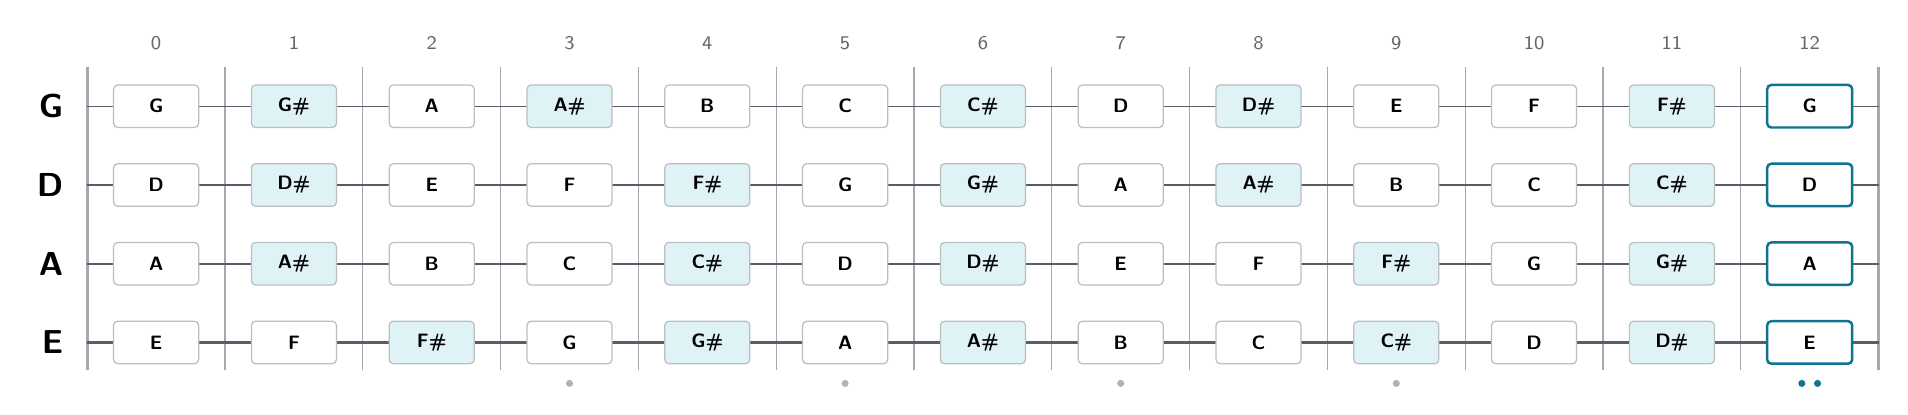
\begin{tikzpicture}[x=1cm,y=1cm]
\node[font=\sffamily\scriptsize,text=Ink!70] at (0.875,4.30) {0};
\node[font=\sffamily\scriptsize,text=Ink!70] at (2.625,4.30) {1};
\node[font=\sffamily\scriptsize,text=Ink!70] at (4.375,4.30) {2};
\node[font=\sffamily\scriptsize,text=Ink!70] at (6.125,4.30) {3};
\node[font=\sffamily\scriptsize,text=Ink!70] at (7.875,4.30) {4};
\node[font=\sffamily\scriptsize,text=Ink!70] at (9.625,4.30) {5};
\node[font=\sffamily\scriptsize,text=Ink!70] at (11.375,4.30) {6};
\node[font=\sffamily\scriptsize,text=Ink!70] at (13.125,4.30) {7};
\node[font=\sffamily\scriptsize,text=Ink!70] at (14.875,4.30) {8};
\node[font=\sffamily\scriptsize,text=Ink!70] at (16.625,4.30) {9};
\node[font=\sffamily\scriptsize,text=Ink!70] at (18.375,4.30) {10};
\node[font=\sffamily\scriptsize,text=Ink!70] at (20.125,4.30) {11};
\node[font=\sffamily\scriptsize,text=Ink!70] at (21.875,4.30) {12};
\draw[Ink!40,line width=1.0pt] (0.000,0.15) -- (0.000,4.0);
\draw[Ink!40,line width=0.45pt] (1.750,0.15) -- (1.750,4.0);
\draw[Ink!40,line width=0.45pt] (3.500,0.15) -- (3.500,4.0);
\draw[Ink!40,line width=0.45pt] (5.250,0.15) -- (5.250,4.0);
\draw[Ink!40,line width=0.45pt] (7.000,0.15) -- (7.000,4.0);
\draw[Ink!40,line width=0.45pt] (8.750,0.15) -- (8.750,4.0);
\draw[Ink!40,line width=0.45pt] (10.500,0.15) -- (10.500,4.0);
\draw[Ink!40,line width=0.45pt] (12.250,0.15) -- (12.250,4.0);
\draw[Ink!40,line width=0.45pt] (14.000,0.15) -- (14.000,4.0);
\draw[Ink!40,line width=0.45pt] (15.750,0.15) -- (15.750,4.0);
\draw[Ink!40,line width=0.45pt] (17.500,0.15) -- (17.500,4.0);
\draw[Ink!40,line width=0.45pt] (19.250,0.15) -- (19.250,4.0);
\draw[Ink!40,line width=0.45pt] (21.000,0.15) -- (21.000,4.0);
\draw[Ink!40,line width=1.0pt] (22.750,0.15) -- (22.750,4.0);
\node[anchor=east,font=\sffamily\bfseries\large] at (-0.18,3.50) {G};
\draw[Ink!75,line width=0.45pt] (0,3.50) -- (22.750,3.50);
\node[rounded corners=1.5pt,minimum width=1.08cm,minimum height=0.54cm,inner sep=1pt,fill=white,draw=Ink!30,line width=0.45pt,font=\sffamily\bfseries\scriptsize] at (0.875,3.50) {G};
\node[rounded corners=1.5pt,minimum width=1.08cm,minimum height=0.54cm,inner sep=1pt,fill=AccentLight,draw=Ink!30,line width=0.45pt,font=\sffamily\bfseries\scriptsize] at (2.625,3.50) {G\#};
\node[rounded corners=1.5pt,minimum width=1.08cm,minimum height=0.54cm,inner sep=1pt,fill=white,draw=Ink!30,line width=0.45pt,font=\sffamily\bfseries\scriptsize] at (4.375,3.50) {A};
\node[rounded corners=1.5pt,minimum width=1.08cm,minimum height=0.54cm,inner sep=1pt,fill=AccentLight,draw=Ink!30,line width=0.45pt,font=\sffamily\bfseries\scriptsize] at (6.125,3.50) {A\#};
\node[rounded corners=1.5pt,minimum width=1.08cm,minimum height=0.54cm,inner sep=1pt,fill=white,draw=Ink!30,line width=0.45pt,font=\sffamily\bfseries\scriptsize] at (7.875,3.50) {B};
\node[rounded corners=1.5pt,minimum width=1.08cm,minimum height=0.54cm,inner sep=1pt,fill=white,draw=Ink!30,line width=0.45pt,font=\sffamily\bfseries\scriptsize] at (9.625,3.50) {C};
\node[rounded corners=1.5pt,minimum width=1.08cm,minimum height=0.54cm,inner sep=1pt,fill=AccentLight,draw=Ink!30,line width=0.45pt,font=\sffamily\bfseries\scriptsize] at (11.375,3.50) {C\#};
\node[rounded corners=1.5pt,minimum width=1.08cm,minimum height=0.54cm,inner sep=1pt,fill=white,draw=Ink!30,line width=0.45pt,font=\sffamily\bfseries\scriptsize] at (13.125,3.50) {D};
\node[rounded corners=1.5pt,minimum width=1.08cm,minimum height=0.54cm,inner sep=1pt,fill=AccentLight,draw=Ink!30,line width=0.45pt,font=\sffamily\bfseries\scriptsize] at (14.875,3.50) {D\#};
\node[rounded corners=1.5pt,minimum width=1.08cm,minimum height=0.54cm,inner sep=1pt,fill=white,draw=Ink!30,line width=0.45pt,font=\sffamily\bfseries\scriptsize] at (16.625,3.50) {E};
\node[rounded corners=1.5pt,minimum width=1.08cm,minimum height=0.54cm,inner sep=1pt,fill=white,draw=Ink!30,line width=0.45pt,font=\sffamily\bfseries\scriptsize] at (18.375,3.50) {F};
\node[rounded corners=1.5pt,minimum width=1.08cm,minimum height=0.54cm,inner sep=1pt,fill=AccentLight,draw=Ink!30,line width=0.45pt,font=\sffamily\bfseries\scriptsize] at (20.125,3.50) {F\#};
\node[rounded corners=1.5pt,minimum width=1.08cm,minimum height=0.54cm,inner sep=1pt,fill=white,draw=Accent,line width=0.9pt,font=\sffamily\bfseries\scriptsize] at (21.875,3.50) {G};
\node[anchor=east,font=\sffamily\bfseries\large] at (-0.18,2.50) {D};
\draw[Ink!75,line width=0.6pt] (0,2.50) -- (22.750,2.50);
\node[rounded corners=1.5pt,minimum width=1.08cm,minimum height=0.54cm,inner sep=1pt,fill=white,draw=Ink!30,line width=0.45pt,font=\sffamily\bfseries\scriptsize] at (0.875,2.50) {D};
\node[rounded corners=1.5pt,minimum width=1.08cm,minimum height=0.54cm,inner sep=1pt,fill=AccentLight,draw=Ink!30,line width=0.45pt,font=\sffamily\bfseries\scriptsize] at (2.625,2.50) {D\#};
\node[rounded corners=1.5pt,minimum width=1.08cm,minimum height=0.54cm,inner sep=1pt,fill=white,draw=Ink!30,line width=0.45pt,font=\sffamily\bfseries\scriptsize] at (4.375,2.50) {E};
\node[rounded corners=1.5pt,minimum width=1.08cm,minimum height=0.54cm,inner sep=1pt,fill=white,draw=Ink!30,line width=0.45pt,font=\sffamily\bfseries\scriptsize] at (6.125,2.50) {F};
\node[rounded corners=1.5pt,minimum width=1.08cm,minimum height=0.54cm,inner sep=1pt,fill=AccentLight,draw=Ink!30,line width=0.45pt,font=\sffamily\bfseries\scriptsize] at (7.875,2.50) {F\#};
\node[rounded corners=1.5pt,minimum width=1.08cm,minimum height=0.54cm,inner sep=1pt,fill=white,draw=Ink!30,line width=0.45pt,font=\sffamily\bfseries\scriptsize] at (9.625,2.50) {G};
\node[rounded corners=1.5pt,minimum width=1.08cm,minimum height=0.54cm,inner sep=1pt,fill=AccentLight,draw=Ink!30,line width=0.45pt,font=\sffamily\bfseries\scriptsize] at (11.375,2.50) {G\#};
\node[rounded corners=1.5pt,minimum width=1.08cm,minimum height=0.54cm,inner sep=1pt,fill=white,draw=Ink!30,line width=0.45pt,font=\sffamily\bfseries\scriptsize] at (13.125,2.50) {A};
\node[rounded corners=1.5pt,minimum width=1.08cm,minimum height=0.54cm,inner sep=1pt,fill=AccentLight,draw=Ink!30,line width=0.45pt,font=\sffamily\bfseries\scriptsize] at (14.875,2.50) {A\#};
\node[rounded corners=1.5pt,minimum width=1.08cm,minimum height=0.54cm,inner sep=1pt,fill=white,draw=Ink!30,line width=0.45pt,font=\sffamily\bfseries\scriptsize] at (16.625,2.50) {B};
\node[rounded corners=1.5pt,minimum width=1.08cm,minimum height=0.54cm,inner sep=1pt,fill=white,draw=Ink!30,line width=0.45pt,font=\sffamily\bfseries\scriptsize] at (18.375,2.50) {C};
\node[rounded corners=1.5pt,minimum width=1.08cm,minimum height=0.54cm,inner sep=1pt,fill=AccentLight,draw=Ink!30,line width=0.45pt,font=\sffamily\bfseries\scriptsize] at (20.125,2.50) {C\#};
\node[rounded corners=1.5pt,minimum width=1.08cm,minimum height=0.54cm,inner sep=1pt,fill=white,draw=Accent,line width=0.9pt,font=\sffamily\bfseries\scriptsize] at (21.875,2.50) {D};
\node[anchor=east,font=\sffamily\bfseries\large] at (-0.18,1.50) {A};
\draw[Ink!75,line width=0.8pt] (0,1.50) -- (22.750,1.50);
\node[rounded corners=1.5pt,minimum width=1.08cm,minimum height=0.54cm,inner sep=1pt,fill=white,draw=Ink!30,line width=0.45pt,font=\sffamily\bfseries\scriptsize] at (0.875,1.50) {A};
\node[rounded corners=1.5pt,minimum width=1.08cm,minimum height=0.54cm,inner sep=1pt,fill=AccentLight,draw=Ink!30,line width=0.45pt,font=\sffamily\bfseries\scriptsize] at (2.625,1.50) {A\#};
\node[rounded corners=1.5pt,minimum width=1.08cm,minimum height=0.54cm,inner sep=1pt,fill=white,draw=Ink!30,line width=0.45pt,font=\sffamily\bfseries\scriptsize] at (4.375,1.50) {B};
\node[rounded corners=1.5pt,minimum width=1.08cm,minimum height=0.54cm,inner sep=1pt,fill=white,draw=Ink!30,line width=0.45pt,font=\sffamily\bfseries\scriptsize] at (6.125,1.50) {C};
\node[rounded corners=1.5pt,minimum width=1.08cm,minimum height=0.54cm,inner sep=1pt,fill=AccentLight,draw=Ink!30,line width=0.45pt,font=\sffamily\bfseries\scriptsize] at (7.875,1.50) {C\#};
\node[rounded corners=1.5pt,minimum width=1.08cm,minimum height=0.54cm,inner sep=1pt,fill=white,draw=Ink!30,line width=0.45pt,font=\sffamily\bfseries\scriptsize] at (9.625,1.50) {D};
\node[rounded corners=1.5pt,minimum width=1.08cm,minimum height=0.54cm,inner sep=1pt,fill=AccentLight,draw=Ink!30,line width=0.45pt,font=\sffamily\bfseries\scriptsize] at (11.375,1.50) {D\#};
\node[rounded corners=1.5pt,minimum width=1.08cm,minimum height=0.54cm,inner sep=1pt,fill=white,draw=Ink!30,line width=0.45pt,font=\sffamily\bfseries\scriptsize] at (13.125,1.50) {E};
\node[rounded corners=1.5pt,minimum width=1.08cm,minimum height=0.54cm,inner sep=1pt,fill=white,draw=Ink!30,line width=0.45pt,font=\sffamily\bfseries\scriptsize] at (14.875,1.50) {F};
\node[rounded corners=1.5pt,minimum width=1.08cm,minimum height=0.54cm,inner sep=1pt,fill=AccentLight,draw=Ink!30,line width=0.45pt,font=\sffamily\bfseries\scriptsize] at (16.625,1.50) {F\#};
\node[rounded corners=1.5pt,minimum width=1.08cm,minimum height=0.54cm,inner sep=1pt,fill=white,draw=Ink!30,line width=0.45pt,font=\sffamily\bfseries\scriptsize] at (18.375,1.50) {G};
\node[rounded corners=1.5pt,minimum width=1.08cm,minimum height=0.54cm,inner sep=1pt,fill=AccentLight,draw=Ink!30,line width=0.45pt,font=\sffamily\bfseries\scriptsize] at (20.125,1.50) {G\#};
\node[rounded corners=1.5pt,minimum width=1.08cm,minimum height=0.54cm,inner sep=1pt,fill=white,draw=Accent,line width=0.9pt,font=\sffamily\bfseries\scriptsize] at (21.875,1.50) {A};
\node[anchor=east,font=\sffamily\bfseries\large] at (-0.18,0.50) {E};
\draw[Ink!75,line width=1.0pt] (0,0.50) -- (22.750,0.50);
\node[rounded corners=1.5pt,minimum width=1.08cm,minimum height=0.54cm,inner sep=1pt,fill=white,draw=Ink!30,line width=0.45pt,font=\sffamily\bfseries\scriptsize] at (0.875,0.50) {E};
\node[rounded corners=1.5pt,minimum width=1.08cm,minimum height=0.54cm,inner sep=1pt,fill=white,draw=Ink!30,line width=0.45pt,font=\sffamily\bfseries\scriptsize] at (2.625,0.50) {F};
\node[rounded corners=1.5pt,minimum width=1.08cm,minimum height=0.54cm,inner sep=1pt,fill=AccentLight,draw=Ink!30,line width=0.45pt,font=\sffamily\bfseries\scriptsize] at (4.375,0.50) {F\#};
\node[rounded corners=1.5pt,minimum width=1.08cm,minimum height=0.54cm,inner sep=1pt,fill=white,draw=Ink!30,line width=0.45pt,font=\sffamily\bfseries\scriptsize] at (6.125,0.50) {G};
\node[rounded corners=1.5pt,minimum width=1.08cm,minimum height=0.54cm,inner sep=1pt,fill=AccentLight,draw=Ink!30,line width=0.45pt,font=\sffamily\bfseries\scriptsize] at (7.875,0.50) {G\#};
\node[rounded corners=1.5pt,minimum width=1.08cm,minimum height=0.54cm,inner sep=1pt,fill=white,draw=Ink!30,line width=0.45pt,font=\sffamily\bfseries\scriptsize] at (9.625,0.50) {A};
\node[rounded corners=1.5pt,minimum width=1.08cm,minimum height=0.54cm,inner sep=1pt,fill=AccentLight,draw=Ink!30,line width=0.45pt,font=\sffamily\bfseries\scriptsize] at (11.375,0.50) {A\#};
\node[rounded corners=1.5pt,minimum width=1.08cm,minimum height=0.54cm,inner sep=1pt,fill=white,draw=Ink!30,line width=0.45pt,font=\sffamily\bfseries\scriptsize] at (13.125,0.50) {B};
\node[rounded corners=1.5pt,minimum width=1.08cm,minimum height=0.54cm,inner sep=1pt,fill=white,draw=Ink!30,line width=0.45pt,font=\sffamily\bfseries\scriptsize] at (14.875,0.50) {C};
\node[rounded corners=1.5pt,minimum width=1.08cm,minimum height=0.54cm,inner sep=1pt,fill=AccentLight,draw=Ink!30,line width=0.45pt,font=\sffamily\bfseries\scriptsize] at (16.625,0.50) {C\#};
\node[rounded corners=1.5pt,minimum width=1.08cm,minimum height=0.54cm,inner sep=1pt,fill=white,draw=Ink!30,line width=0.45pt,font=\sffamily\bfseries\scriptsize] at (18.375,0.50) {D};
\node[rounded corners=1.5pt,minimum width=1.08cm,minimum height=0.54cm,inner sep=1pt,fill=AccentLight,draw=Ink!30,line width=0.45pt,font=\sffamily\bfseries\scriptsize] at (20.125,0.50) {D\#};
\node[rounded corners=1.5pt,minimum width=1.08cm,minimum height=0.54cm,inner sep=1pt,fill=white,draw=Accent,line width=0.9pt,font=\sffamily\bfseries\scriptsize] at (21.875,0.50) {E};
\fill[Ink!35] (6.125,-0.02) circle (0.045);
\fill[Ink!35] (9.625,-0.02) circle (0.045);
\fill[Ink!35] (13.125,-0.02) circle (0.045);
\fill[Ink!35] (16.625,-0.02) circle (0.045);
\fill[Accent] (21.775,-0.02) circle (0.045);
\fill[Accent] (21.975,-0.02) circle (0.045);
\end{tikzpicture}
\end{center}\vspace{4mm}
{\sffamily\bfseries\large Frets 12--24}\par
\begin{center}
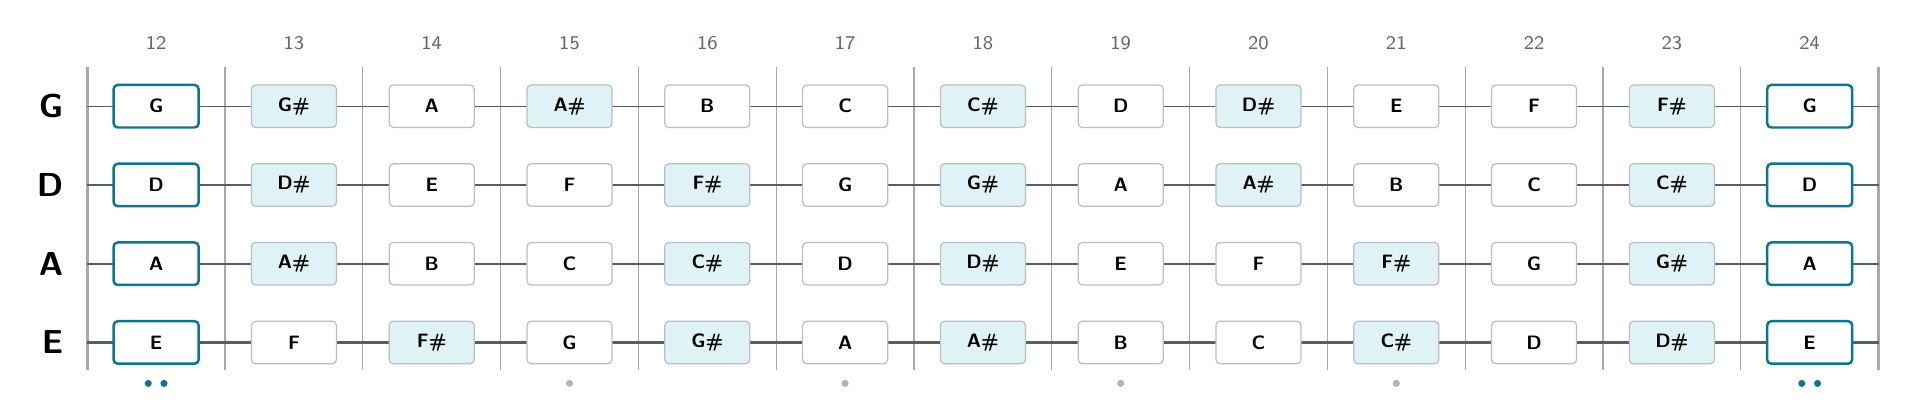
\begin{tikzpicture}[x=1cm,y=1cm]
\node[font=\sffamily\scriptsize,text=Ink!70] at (0.875,4.30) {12};
\node[font=\sffamily\scriptsize,text=Ink!70] at (2.625,4.30) {13};
\node[font=\sffamily\scriptsize,text=Ink!70] at (4.375,4.30) {14};
\node[font=\sffamily\scriptsize,text=Ink!70] at (6.125,4.30) {15};
\node[font=\sffamily\scriptsize,text=Ink!70] at (7.875,4.30) {16};
\node[font=\sffamily\scriptsize,text=Ink!70] at (9.625,4.30) {17};
\node[font=\sffamily\scriptsize,text=Ink!70] at (11.375,4.30) {18};
\node[font=\sffamily\scriptsize,text=Ink!70] at (13.125,4.30) {19};
\node[font=\sffamily\scriptsize,text=Ink!70] at (14.875,4.30) {20};
\node[font=\sffamily\scriptsize,text=Ink!70] at (16.625,4.30) {21};
\node[font=\sffamily\scriptsize,text=Ink!70] at (18.375,4.30) {22};
\node[font=\sffamily\scriptsize,text=Ink!70] at (20.125,4.30) {23};
\node[font=\sffamily\scriptsize,text=Ink!70] at (21.875,4.30) {24};
\draw[Ink!40,line width=1.0pt] (0.000,0.15) -- (0.000,4.0);
\draw[Ink!40,line width=0.45pt] (1.750,0.15) -- (1.750,4.0);
\draw[Ink!40,line width=0.45pt] (3.500,0.15) -- (3.500,4.0);
\draw[Ink!40,line width=0.45pt] (5.250,0.15) -- (5.250,4.0);
\draw[Ink!40,line width=0.45pt] (7.000,0.15) -- (7.000,4.0);
\draw[Ink!40,line width=0.45pt] (8.750,0.15) -- (8.750,4.0);
\draw[Ink!40,line width=0.45pt] (10.500,0.15) -- (10.500,4.0);
\draw[Ink!40,line width=0.45pt] (12.250,0.15) -- (12.250,4.0);
\draw[Ink!40,line width=0.45pt] (14.000,0.15) -- (14.000,4.0);
\draw[Ink!40,line width=0.45pt] (15.750,0.15) -- (15.750,4.0);
\draw[Ink!40,line width=0.45pt] (17.500,0.15) -- (17.500,4.0);
\draw[Ink!40,line width=0.45pt] (19.250,0.15) -- (19.250,4.0);
\draw[Ink!40,line width=0.45pt] (21.000,0.15) -- (21.000,4.0);
\draw[Ink!40,line width=1.0pt] (22.750,0.15) -- (22.750,4.0);
\node[anchor=east,font=\sffamily\bfseries\large] at (-0.18,3.50) {G};
\draw[Ink!75,line width=0.45pt] (0,3.50) -- (22.750,3.50);
\node[rounded corners=1.5pt,minimum width=1.08cm,minimum height=0.54cm,inner sep=1pt,fill=white,draw=Accent,line width=0.9pt,font=\sffamily\bfseries\scriptsize] at (0.875,3.50) {G};
\node[rounded corners=1.5pt,minimum width=1.08cm,minimum height=0.54cm,inner sep=1pt,fill=AccentLight,draw=Ink!30,line width=0.45pt,font=\sffamily\bfseries\scriptsize] at (2.625,3.50) {G\#};
\node[rounded corners=1.5pt,minimum width=1.08cm,minimum height=0.54cm,inner sep=1pt,fill=white,draw=Ink!30,line width=0.45pt,font=\sffamily\bfseries\scriptsize] at (4.375,3.50) {A};
\node[rounded corners=1.5pt,minimum width=1.08cm,minimum height=0.54cm,inner sep=1pt,fill=AccentLight,draw=Ink!30,line width=0.45pt,font=\sffamily\bfseries\scriptsize] at (6.125,3.50) {A\#};
\node[rounded corners=1.5pt,minimum width=1.08cm,minimum height=0.54cm,inner sep=1pt,fill=white,draw=Ink!30,line width=0.45pt,font=\sffamily\bfseries\scriptsize] at (7.875,3.50) {B};
\node[rounded corners=1.5pt,minimum width=1.08cm,minimum height=0.54cm,inner sep=1pt,fill=white,draw=Ink!30,line width=0.45pt,font=\sffamily\bfseries\scriptsize] at (9.625,3.50) {C};
\node[rounded corners=1.5pt,minimum width=1.08cm,minimum height=0.54cm,inner sep=1pt,fill=AccentLight,draw=Ink!30,line width=0.45pt,font=\sffamily\bfseries\scriptsize] at (11.375,3.50) {C\#};
\node[rounded corners=1.5pt,minimum width=1.08cm,minimum height=0.54cm,inner sep=1pt,fill=white,draw=Ink!30,line width=0.45pt,font=\sffamily\bfseries\scriptsize] at (13.125,3.50) {D};
\node[rounded corners=1.5pt,minimum width=1.08cm,minimum height=0.54cm,inner sep=1pt,fill=AccentLight,draw=Ink!30,line width=0.45pt,font=\sffamily\bfseries\scriptsize] at (14.875,3.50) {D\#};
\node[rounded corners=1.5pt,minimum width=1.08cm,minimum height=0.54cm,inner sep=1pt,fill=white,draw=Ink!30,line width=0.45pt,font=\sffamily\bfseries\scriptsize] at (16.625,3.50) {E};
\node[rounded corners=1.5pt,minimum width=1.08cm,minimum height=0.54cm,inner sep=1pt,fill=white,draw=Ink!30,line width=0.45pt,font=\sffamily\bfseries\scriptsize] at (18.375,3.50) {F};
\node[rounded corners=1.5pt,minimum width=1.08cm,minimum height=0.54cm,inner sep=1pt,fill=AccentLight,draw=Ink!30,line width=0.45pt,font=\sffamily\bfseries\scriptsize] at (20.125,3.50) {F\#};
\node[rounded corners=1.5pt,minimum width=1.08cm,minimum height=0.54cm,inner sep=1pt,fill=white,draw=Accent,line width=0.9pt,font=\sffamily\bfseries\scriptsize] at (21.875,3.50) {G};
\node[anchor=east,font=\sffamily\bfseries\large] at (-0.18,2.50) {D};
\draw[Ink!75,line width=0.6pt] (0,2.50) -- (22.750,2.50);
\node[rounded corners=1.5pt,minimum width=1.08cm,minimum height=0.54cm,inner sep=1pt,fill=white,draw=Accent,line width=0.9pt,font=\sffamily\bfseries\scriptsize] at (0.875,2.50) {D};
\node[rounded corners=1.5pt,minimum width=1.08cm,minimum height=0.54cm,inner sep=1pt,fill=AccentLight,draw=Ink!30,line width=0.45pt,font=\sffamily\bfseries\scriptsize] at (2.625,2.50) {D\#};
\node[rounded corners=1.5pt,minimum width=1.08cm,minimum height=0.54cm,inner sep=1pt,fill=white,draw=Ink!30,line width=0.45pt,font=\sffamily\bfseries\scriptsize] at (4.375,2.50) {E};
\node[rounded corners=1.5pt,minimum width=1.08cm,minimum height=0.54cm,inner sep=1pt,fill=white,draw=Ink!30,line width=0.45pt,font=\sffamily\bfseries\scriptsize] at (6.125,2.50) {F};
\node[rounded corners=1.5pt,minimum width=1.08cm,minimum height=0.54cm,inner sep=1pt,fill=AccentLight,draw=Ink!30,line width=0.45pt,font=\sffamily\bfseries\scriptsize] at (7.875,2.50) {F\#};
\node[rounded corners=1.5pt,minimum width=1.08cm,minimum height=0.54cm,inner sep=1pt,fill=white,draw=Ink!30,line width=0.45pt,font=\sffamily\bfseries\scriptsize] at (9.625,2.50) {G};
\node[rounded corners=1.5pt,minimum width=1.08cm,minimum height=0.54cm,inner sep=1pt,fill=AccentLight,draw=Ink!30,line width=0.45pt,font=\sffamily\bfseries\scriptsize] at (11.375,2.50) {G\#};
\node[rounded corners=1.5pt,minimum width=1.08cm,minimum height=0.54cm,inner sep=1pt,fill=white,draw=Ink!30,line width=0.45pt,font=\sffamily\bfseries\scriptsize] at (13.125,2.50) {A};
\node[rounded corners=1.5pt,minimum width=1.08cm,minimum height=0.54cm,inner sep=1pt,fill=AccentLight,draw=Ink!30,line width=0.45pt,font=\sffamily\bfseries\scriptsize] at (14.875,2.50) {A\#};
\node[rounded corners=1.5pt,minimum width=1.08cm,minimum height=0.54cm,inner sep=1pt,fill=white,draw=Ink!30,line width=0.45pt,font=\sffamily\bfseries\scriptsize] at (16.625,2.50) {B};
\node[rounded corners=1.5pt,minimum width=1.08cm,minimum height=0.54cm,inner sep=1pt,fill=white,draw=Ink!30,line width=0.45pt,font=\sffamily\bfseries\scriptsize] at (18.375,2.50) {C};
\node[rounded corners=1.5pt,minimum width=1.08cm,minimum height=0.54cm,inner sep=1pt,fill=AccentLight,draw=Ink!30,line width=0.45pt,font=\sffamily\bfseries\scriptsize] at (20.125,2.50) {C\#};
\node[rounded corners=1.5pt,minimum width=1.08cm,minimum height=0.54cm,inner sep=1pt,fill=white,draw=Accent,line width=0.9pt,font=\sffamily\bfseries\scriptsize] at (21.875,2.50) {D};
\node[anchor=east,font=\sffamily\bfseries\large] at (-0.18,1.50) {A};
\draw[Ink!75,line width=0.8pt] (0,1.50) -- (22.750,1.50);
\node[rounded corners=1.5pt,minimum width=1.08cm,minimum height=0.54cm,inner sep=1pt,fill=white,draw=Accent,line width=0.9pt,font=\sffamily\bfseries\scriptsize] at (0.875,1.50) {A};
\node[rounded corners=1.5pt,minimum width=1.08cm,minimum height=0.54cm,inner sep=1pt,fill=AccentLight,draw=Ink!30,line width=0.45pt,font=\sffamily\bfseries\scriptsize] at (2.625,1.50) {A\#};
\node[rounded corners=1.5pt,minimum width=1.08cm,minimum height=0.54cm,inner sep=1pt,fill=white,draw=Ink!30,line width=0.45pt,font=\sffamily\bfseries\scriptsize] at (4.375,1.50) {B};
\node[rounded corners=1.5pt,minimum width=1.08cm,minimum height=0.54cm,inner sep=1pt,fill=white,draw=Ink!30,line width=0.45pt,font=\sffamily\bfseries\scriptsize] at (6.125,1.50) {C};
\node[rounded corners=1.5pt,minimum width=1.08cm,minimum height=0.54cm,inner sep=1pt,fill=AccentLight,draw=Ink!30,line width=0.45pt,font=\sffamily\bfseries\scriptsize] at (7.875,1.50) {C\#};
\node[rounded corners=1.5pt,minimum width=1.08cm,minimum height=0.54cm,inner sep=1pt,fill=white,draw=Ink!30,line width=0.45pt,font=\sffamily\bfseries\scriptsize] at (9.625,1.50) {D};
\node[rounded corners=1.5pt,minimum width=1.08cm,minimum height=0.54cm,inner sep=1pt,fill=AccentLight,draw=Ink!30,line width=0.45pt,font=\sffamily\bfseries\scriptsize] at (11.375,1.50) {D\#};
\node[rounded corners=1.5pt,minimum width=1.08cm,minimum height=0.54cm,inner sep=1pt,fill=white,draw=Ink!30,line width=0.45pt,font=\sffamily\bfseries\scriptsize] at (13.125,1.50) {E};
\node[rounded corners=1.5pt,minimum width=1.08cm,minimum height=0.54cm,inner sep=1pt,fill=white,draw=Ink!30,line width=0.45pt,font=\sffamily\bfseries\scriptsize] at (14.875,1.50) {F};
\node[rounded corners=1.5pt,minimum width=1.08cm,minimum height=0.54cm,inner sep=1pt,fill=AccentLight,draw=Ink!30,line width=0.45pt,font=\sffamily\bfseries\scriptsize] at (16.625,1.50) {F\#};
\node[rounded corners=1.5pt,minimum width=1.08cm,minimum height=0.54cm,inner sep=1pt,fill=white,draw=Ink!30,line width=0.45pt,font=\sffamily\bfseries\scriptsize] at (18.375,1.50) {G};
\node[rounded corners=1.5pt,minimum width=1.08cm,minimum height=0.54cm,inner sep=1pt,fill=AccentLight,draw=Ink!30,line width=0.45pt,font=\sffamily\bfseries\scriptsize] at (20.125,1.50) {G\#};
\node[rounded corners=1.5pt,minimum width=1.08cm,minimum height=0.54cm,inner sep=1pt,fill=white,draw=Accent,line width=0.9pt,font=\sffamily\bfseries\scriptsize] at (21.875,1.50) {A};
\node[anchor=east,font=\sffamily\bfseries\large] at (-0.18,0.50) {E};
\draw[Ink!75,line width=1.0pt] (0,0.50) -- (22.750,0.50);
\node[rounded corners=1.5pt,minimum width=1.08cm,minimum height=0.54cm,inner sep=1pt,fill=white,draw=Accent,line width=0.9pt,font=\sffamily\bfseries\scriptsize] at (0.875,0.50) {E};
\node[rounded corners=1.5pt,minimum width=1.08cm,minimum height=0.54cm,inner sep=1pt,fill=white,draw=Ink!30,line width=0.45pt,font=\sffamily\bfseries\scriptsize] at (2.625,0.50) {F};
\node[rounded corners=1.5pt,minimum width=1.08cm,minimum height=0.54cm,inner sep=1pt,fill=AccentLight,draw=Ink!30,line width=0.45pt,font=\sffamily\bfseries\scriptsize] at (4.375,0.50) {F\#};
\node[rounded corners=1.5pt,minimum width=1.08cm,minimum height=0.54cm,inner sep=1pt,fill=white,draw=Ink!30,line width=0.45pt,font=\sffamily\bfseries\scriptsize] at (6.125,0.50) {G};
\node[rounded corners=1.5pt,minimum width=1.08cm,minimum height=0.54cm,inner sep=1pt,fill=AccentLight,draw=Ink!30,line width=0.45pt,font=\sffamily\bfseries\scriptsize] at (7.875,0.50) {G\#};
\node[rounded corners=1.5pt,minimum width=1.08cm,minimum height=0.54cm,inner sep=1pt,fill=white,draw=Ink!30,line width=0.45pt,font=\sffamily\bfseries\scriptsize] at (9.625,0.50) {A};
\node[rounded corners=1.5pt,minimum width=1.08cm,minimum height=0.54cm,inner sep=1pt,fill=AccentLight,draw=Ink!30,line width=0.45pt,font=\sffamily\bfseries\scriptsize] at (11.375,0.50) {A\#};
\node[rounded corners=1.5pt,minimum width=1.08cm,minimum height=0.54cm,inner sep=1pt,fill=white,draw=Ink!30,line width=0.45pt,font=\sffamily\bfseries\scriptsize] at (13.125,0.50) {B};
\node[rounded corners=1.5pt,minimum width=1.08cm,minimum height=0.54cm,inner sep=1pt,fill=white,draw=Ink!30,line width=0.45pt,font=\sffamily\bfseries\scriptsize] at (14.875,0.50) {C};
\node[rounded corners=1.5pt,minimum width=1.08cm,minimum height=0.54cm,inner sep=1pt,fill=AccentLight,draw=Ink!30,line width=0.45pt,font=\sffamily\bfseries\scriptsize] at (16.625,0.50) {C\#};
\node[rounded corners=1.5pt,minimum width=1.08cm,minimum height=0.54cm,inner sep=1pt,fill=white,draw=Ink!30,line width=0.45pt,font=\sffamily\bfseries\scriptsize] at (18.375,0.50) {D};
\node[rounded corners=1.5pt,minimum width=1.08cm,minimum height=0.54cm,inner sep=1pt,fill=AccentLight,draw=Ink!30,line width=0.45pt,font=\sffamily\bfseries\scriptsize] at (20.125,0.50) {D\#};
\node[rounded corners=1.5pt,minimum width=1.08cm,minimum height=0.54cm,inner sep=1pt,fill=white,draw=Accent,line width=0.9pt,font=\sffamily\bfseries\scriptsize] at (21.875,0.50) {E};
\fill[Ink!35] (6.125,-0.02) circle (0.045);
\fill[Ink!35] (9.625,-0.02) circle (0.045);
\fill[Ink!35] (13.125,-0.02) circle (0.045);
\fill[Ink!35] (16.625,-0.02) circle (0.045);
\fill[Accent] (0.775,-0.02) circle (0.045);
\fill[Accent] (0.975,-0.02) circle (0.045);
\fill[Accent] (21.775,-0.02) circle (0.045);
\fill[Accent] (21.975,-0.02) circle (0.045);
\end{tikzpicture}
\end{center}\end{landscape}
\clearpage
\clearpage
\section{Interval map on the fretboard}
\begin{keybox}
Intervals are the reusable geometry behind scales, arpeggios and basslines. The diagram uses D at A-string fret 5 and shows one nearby occurrence of every interval through the octave.
\end{keybox}
\begin{center}
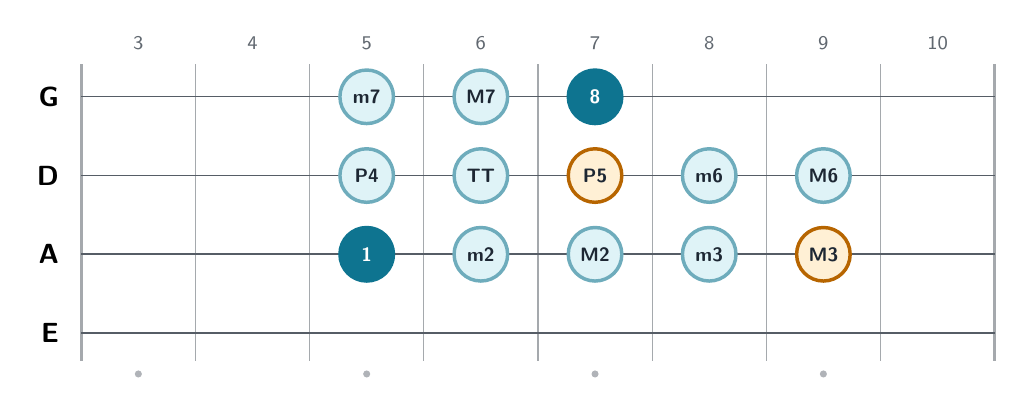
\begin{tikzpicture}[x=1cm,y=1cm,>=stealth]
\node[font=\sffamily\scriptsize,text=Ink!70] at (0.725,4.18) {3};
\node[font=\sffamily\scriptsize,text=Ink!70] at (2.175,4.18) {4};
\node[font=\sffamily\scriptsize,text=Ink!70] at (3.625,4.18) {5};
\node[font=\sffamily\scriptsize,text=Ink!70] at (5.075,4.18) {6};
\node[font=\sffamily\scriptsize,text=Ink!70] at (6.525,4.18) {7};
\node[font=\sffamily\scriptsize,text=Ink!70] at (7.975,4.18) {8};
\node[font=\sffamily\scriptsize,text=Ink!70] at (9.425,4.18) {9};
\node[font=\sffamily\scriptsize,text=Ink!70] at (10.875,4.18) {10};
\draw[Ink!40,line width=1.0pt] (0.000,0.15) -- (0.000,3.92);
\draw[Ink!40,line width=0.45pt] (1.450,0.15) -- (1.450,3.92);
\draw[Ink!40,line width=0.45pt] (2.900,0.15) -- (2.900,3.92);
\draw[Ink!40,line width=0.45pt] (4.350,0.15) -- (4.350,3.92);
\draw[Ink!40,line width=0.45pt] (5.800,0.15) -- (5.800,3.92);
\draw[Ink!40,line width=0.45pt] (7.250,0.15) -- (7.250,3.92);
\draw[Ink!40,line width=0.45pt] (8.700,0.15) -- (8.700,3.92);
\draw[Ink!40,line width=0.45pt] (10.150,0.15) -- (10.150,3.92);
\draw[Ink!40,line width=1.0pt] (11.600,0.15) -- (11.600,3.92);
\node[anchor=east,font=\sffamily\bfseries] at (-0.16,3.50) {G};
\draw[Ink!75,line width=0.45pt] (0,3.50) -- (11.600,3.50);
\node[anchor=east,font=\sffamily\bfseries] at (-0.16,2.50) {D};
\draw[Ink!75,line width=0.6pt] (0,2.50) -- (11.600,2.50);
\node[anchor=east,font=\sffamily\bfseries] at (-0.16,1.50) {A};
\draw[Ink!75,line width=0.8pt] (0,1.50) -- (11.600,1.50);
\node[anchor=east,font=\sffamily\bfseries] at (-0.16,0.50) {E};
\draw[Ink!75,line width=1.0pt] (0,0.50) -- (11.600,0.50);
\fill[Ink!35] (0.725,-0.02) circle (0.045);
\fill[Ink!35] (3.625,-0.02) circle (0.045);
\fill[Ink!35] (6.525,-0.02) circle (0.045);
\fill[Ink!35] (9.425,-0.02) circle (0.045);
\node[circle,minimum size=0.68cm,inner sep=0pt,fill=Accent,draw=Accent,text=white,line width=1.25pt,font=\sffamily\bfseries\scriptsize] at (3.625,1.500) {1};
\node[circle,minimum size=0.68cm,inner sep=0pt,fill=AccentLight,draw=Accent!60,text=Ink,line width=1.25pt,font=\sffamily\bfseries\scriptsize] at (5.075,1.500) {m2};
\node[circle,minimum size=0.68cm,inner sep=0pt,fill=AccentLight,draw=Accent!60,text=Ink,line width=1.25pt,font=\sffamily\bfseries\scriptsize] at (6.525,1.500) {M2};
\node[circle,minimum size=0.68cm,inner sep=0pt,fill=AccentLight,draw=Accent!60,text=Ink,line width=1.25pt,font=\sffamily\bfseries\scriptsize] at (7.975,1.500) {m3};
\node[circle,minimum size=0.68cm,inner sep=0pt,fill=ChordLight,draw=Chord,text=Ink,line width=1.25pt,font=\sffamily\bfseries\scriptsize] at (9.425,1.500) {M3};
\node[circle,minimum size=0.68cm,inner sep=0pt,fill=AccentLight,draw=Accent!60,text=Ink,line width=1.25pt,font=\sffamily\bfseries\scriptsize] at (3.625,2.500) {P4};
\node[circle,minimum size=0.68cm,inner sep=0pt,fill=AccentLight,draw=Accent!60,text=Ink,line width=1.25pt,font=\sffamily\bfseries\scriptsize] at (5.075,2.500) {TT};
\node[circle,minimum size=0.68cm,inner sep=0pt,fill=ChordLight,draw=Chord,text=Ink,line width=1.25pt,font=\sffamily\bfseries\scriptsize] at (6.525,2.500) {P5};
\node[circle,minimum size=0.68cm,inner sep=0pt,fill=AccentLight,draw=Accent!60,text=Ink,line width=1.25pt,font=\sffamily\bfseries\scriptsize] at (7.975,2.500) {m6};
\node[circle,minimum size=0.68cm,inner sep=0pt,fill=AccentLight,draw=Accent!60,text=Ink,line width=1.25pt,font=\sffamily\bfseries\scriptsize] at (9.425,2.500) {M6};
\node[circle,minimum size=0.68cm,inner sep=0pt,fill=AccentLight,draw=Accent!60,text=Ink,line width=1.25pt,font=\sffamily\bfseries\scriptsize] at (3.625,3.500) {m7};
\node[circle,minimum size=0.68cm,inner sep=0pt,fill=AccentLight,draw=Accent!60,text=Ink,line width=1.25pt,font=\sffamily\bfseries\scriptsize] at (5.075,3.500) {M7};
\node[circle,minimum size=0.68cm,inner sep=0pt,fill=Accent,draw=Accent,text=white,line width=1.25pt,font=\sffamily\bfseries\scriptsize] at (6.525,3.500) {8};
\end{tikzpicture}
\end{center}
\begin{longtable}{>{\bfseries}p{2.6cm}p{2.2cm}p{3.2cm}p{7.0cm}}
\toprule
Interval & Semitones & Degree spelling & Common bass function \\
\midrule
\endhead
Minor second & 1 & $\flat2$ & Chromatic approach, Phrygian colour, strongest adjacent tension. \\
Major second & 2 & 2 & Scale connection and suspended colour. \\
Minor third & 3 & $\flat3$ & Defines minor triads and minor-seven chords. \\
Major third & 4 & 3 & Defines major triads and dominant chords. \\
Perfect fourth & 5 & 4 & Strong scale tone; inversion of the perfect fifth. \\
Tritone & 6 & $\sharp4/\flat5$ & Dominant tension and diminished harmony. \\
Perfect fifth & 7 & 5 & Stable support; the most common partner to the root. \\
Minor sixth & 8 & $\flat6$ & Natural-minor colour and approach tone. \\
Major sixth & 9 & 6 & Dorian, major-pentatonic and Latin colour. \\
Minor seventh & 10 & $\flat7$ & Dominant-seven and minor-seven harmony. \\
Major seventh & 11 & 7 & Major-seven colour and leading tone. \\
Octave & 12 & 8 & Same pitch class in a higher register. \\
\bottomrule
\end{longtable}

\clearpage
\section{Reading and rhythm reference}
\subsection{Bass clef and written range}
\begin{tabularx}{\textwidth}{>{\bfseries\sffamily}p{3.6cm}Y}
\toprule
Bass-clef lines & G--B--D--F--A, from the lowest line upward. \\
Bass-clef spaces & A--C--E--G, from the lowest space upward. \\
Open strings & E--A--D--G. Written bass-guitar notation sounds one octave lower than written. \\
TAB orientation & G is the top line; E is the bottom line. A number is the fret to press. \\
Accidentals & A sharp or flat applies through the current measure unless cancelled or replaced. \\
Tie & Joins identical pitches into one sustained duration. \\
Dot & Adds half of the original note value. A dotted quarter equals three eighth notes. \\
\bottomrule
\end{tabularx}
\begin{center}
\begingroup
\setlength{\parindent}{0pt}
\begin{minipage}{0.88\textwidth}
{\sffamily\bfseries\small Rhythmic values on D: whole, halves, quarters and eighths}\par\vspace{-1mm}
\begin{music}
\instrumentnumber{1}
\setstaffs1{1}
\setclef1{\bass}
\generalmeter{\meterfrac44}
\nobarnumbers
\nostartrule
\startextract
\Notes\wh K\en
\bar
\Notes\hu K\hu K\en
\bar
\Notes\qu K\qu K\qu K\qu K\en
\bar
\Notes\cu K\cu K\cu K\cu K\cu K\cu K\cu K\cu K\en
\zendextract
\end{music}
\end{minipage}
\endgroup
\end{center}
\begin{center}
\begin{tabular}{>{\bfseries}l C{2.6cm} C{3.2cm} C{3.2cm}}
\toprule
Value & Length in 4/4 & Notes per quarter-note beat & Matching rest \\
\midrule
Whole & 4 beats & $1/4$ & Whole rest \\
Half & 2 beats & $1/2$ & Half rest \\
Quarter & 1 beat & 1 & Quarter rest \\
Eighth & $1/2$ beat & 2 & Eighth rest \\
Sixteenth & $1/4$ beat & 4 & Sixteenth rest \\
\bottomrule
\end{tabular}
\end{center}

\subsection{Common articulation and TAB markings}
\begin{tabularx}{\textwidth}{>{\bfseries\sffamily}p{3.0cm}p{2.4cm}Y}
\toprule
Technique & Common marking & Meaning \\
\midrule
Staccato & dot above/below note & Shorten the note while preserving its rhythmic position. \\
Accent & $>$ & Stronger attack. \\
Dead / ghost note & x & Muted percussive attack without a clear pitch. \\
Slide & / or $\backslash$ in TAB & Maintain contact while moving to the destination fret. \\
Hammer-on / pull-off & h / p in TAB & Sound the following note mainly with the fretting hand. \\
Let ring & tie or ``let ring'' & Sustain until the indicated release point. \\
\bottomrule
\end{tabularx}

\clearpage
\section{Chord symbols and chord construction}
\begin{longtable}{>{\bfseries}p{3.0cm}p{3.0cm}p{4.2cm}p{5.8cm}}
\toprule
Chord type & Example symbol & Formula & Bass priority \\
\midrule
\endhead
Major triad & C & 1--3--5 & Root first; third states major; fifth supplies stability. \\
Minor triad & Cm & 1--$\flat3$--5 & Root and minor third define the sound. \\
Power chord & C5 & 1--5 & Neither major nor minor because the third is absent. \\
Suspended 2 & Csus2 & 1--2--5 & Avoid adding a third unless the harmony resolves. \\
Suspended 4 & Csus4 & 1--4--5 & Fourth replaces the third. \\
Major seven & Cmaj7 & 1--3--5--7 & Major seventh is the characteristic colour. \\
Dominant seven & C7 & 1--3--5--$\flat7$ & Third and flat seventh form the defining tritone. \\
Minor seven & Cm7 & 1--$\flat3$--5--$\flat7$ & Root, flat third and flat seventh identify the chord. \\
Half-diminished & Cm7$\flat5$ & 1--$\flat3$--$\flat5$--$\flat7$ & Flat fifth is essential. \\
Diminished seven & Cdim7 & 1--$\flat3$--$\flat5$--$\flat\flat7$ & Symmetrical stack of minor thirds. \\
Augmented & Caug / C+ & 1--3--$\sharp5$ & Raised fifth creates the instability. \\
\bottomrule
\end{longtable}

\section{Diatonic harmony}
\subsection{Major key}
\begin{center}
\begin{tabular}{C{1.7cm}C{1.7cm}C{1.7cm}C{1.7cm}C{1.7cm}C{1.7cm}C{1.7cm}}
\toprule
I & ii & iii & IV & V & vi & vii$^\circ$ \\
Major & minor & minor & Major & Major & minor & diminished \\
maj7 & m7 & m7 & maj7 & 7 & m7 & m7$\flat5$ \\
\bottomrule
\end{tabular}
\end{center}
\subsection{Natural minor key}
\begin{center}
\begin{tabular}{C{1.7cm}C{1.7cm}C{1.7cm}C{1.7cm}C{1.7cm}C{1.7cm}C{1.7cm}}
\toprule
i & ii$^\circ$ & III & iv & v & VI & VII \\
minor & diminished & Major & minor & minor & Major & Major \\
m7 & m7$\flat5$ & maj7 & m7 & m7 & maj7 & 7 \\
\bottomrule
\end{tabular}
\end{center}
\begin{neutralbox}
In functional minor harmony the V chord is commonly changed from minor to dominant by raising scale degree 7. This is the practical reason harmonic minor is important.
\end{neutralbox}

\clearpage
\section{Key signatures and relative minors}
\begin{longtable}{>{\bfseries}p{2.4cm}p{3.0cm}p{3.1cm}p{3.2cm}p{4.3cm}}
\toprule
Major key & Signature & Relative minor & Main notes altered & Useful bass reference \\
\midrule
\endhead
C & none & A minor & none & All natural notes. \\
G & 1 sharp & E minor & F$\sharp$ & G major / E natural minor. \\
D & 2 sharps & B minor & F$\sharp$, C$\sharp$ & The example key used throughout the scale atlas. \\
A & 3 sharps & F$\sharp$ minor & F$\sharp$, C$\sharp$, G$\sharp$ & Common guitar and bass key. \\
E & 4 sharps & C$\sharp$ minor & F$\sharp$, C$\sharp$, G$\sharp$, D$\sharp$ & Open E string is the tonic. \\
F & 1 flat & D minor & B$\flat$ & Common horn and Latin key. \\
B$\flat$ & 2 flats & G minor & B$\flat$, E$\flat$ & Common brass and salsa key. \\
E$\flat$ & 3 flats & C minor & B$\flat$, E$\flat$, A$\flat$ & Common horn, soul and salsa key. \\
A$\flat$ & 4 flats & F minor & B$\flat$, E$\flat$, A$\flat$, D$\flat$ & Frequent keyboard and horn key. \\
\bottomrule
\end{longtable}
\begin{keybox}
\textbf{Transposition rule:} a movable fingering keeps the same interval structure. Shift every note by the same number of frets, then rename the root and scale degrees.
\end{keybox}

\section{Scale index}
\begin{longtable}{>{\bfseries}p{3.2cm}p{4.2cm}p{4.0cm}p{4.0cm}}
\toprule
Scale & Degree formula & Main identifying tone & Typical harmonic fit \\
\midrule
\endhead
Major / Ionian & 1 2 3 4 5 6 7 & Natural 3 and 7 & Major, major 7 \\
Natural minor / Aeolian & 1 2 $\flat3$ 4 5 $\flat6$ $\flat7$ & $\flat6$ & Minor, minor 7 \\
Dorian & 1 2 $\flat3$ 4 5 6 $\flat7$ & Natural 6 & Minor 7 \\
Phrygian & 1 $\flat2$ $\flat3$ 4 5 $\flat6$ $\flat7$ & $\flat2$ & Minor with lowered-second colour \\
Lydian & 1 2 3 $\sharp4$ 5 6 7 & $\sharp4$ & Major $\sharp11$ \\
Mixolydian & 1 2 3 4 5 6 $\flat7$ & $\flat7$ & Dominant 7 \\
Locrian & 1 $\flat2$ $\flat3$ 4 $\flat5$ $\flat6$ $\flat7$ & $\flat5$ & Half-diminished \\
Harmonic minor & 1 2 $\flat3$ 4 5 $\flat6$ 7 & Raised 7 & Minor key with dominant V7 \\
Melodic minor & 1 2 $\flat3$ 4 5 6 7 & Natural 6 and 7 & Minor-major 7, modern jazz \\
Major pentatonic & 1 2 3 5 6 & Omits 4 and 7 & Major harmony \\
Minor pentatonic & 1 $\flat3$ 4 5 $\flat7$ & Compact minor set & Minor harmony \\
Blues & 1 $\flat3$ 4 $\flat5$ 5 $\flat7$ & Added $\flat5$ & Blues vocabulary \\
\bottomrule
\end{longtable}

\begin{neutralbox}
The scale atlas uses D as the example root because A-string fret 5 gives a clear, movable mid-neck position. The degree formula, not the note spelling, is the transposable information.
\end{neutralbox}
\clearpage
\section{Major (Ionian)}\label{scale:major}
\begin{tabularx}{\textwidth}{>{\bfseries\sffamily}p{2.8cm}Y}
Formula & 1 2 3 4 5 6 7 \\
Step pattern & W -- W -- H -- W -- W -- W -- H \\
D example & D--E--F\#--G--A--B--C\#--D \\
\end{tabularx}
\begin{center}
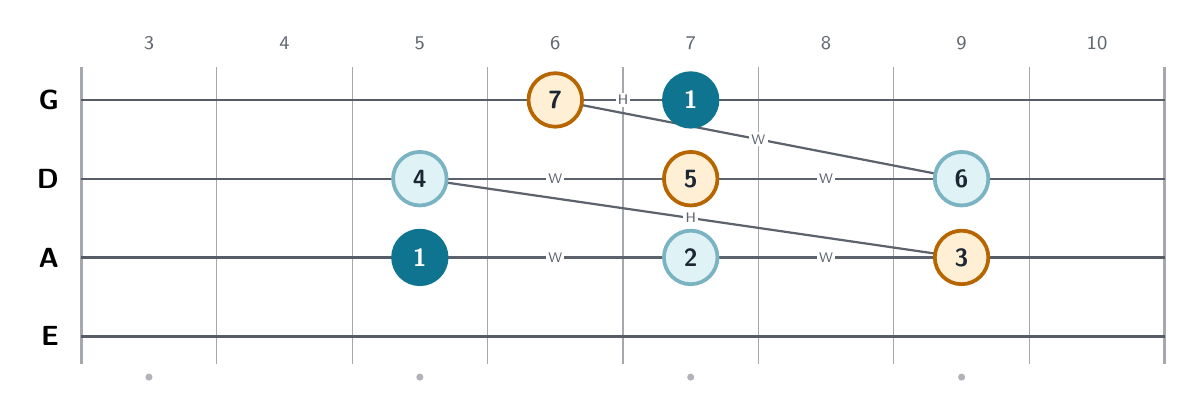
\begin{tikzpicture}[x=1cm,y=1cm,>=stealth]
\node[font=\sffamily\scriptsize,text=Ink!70] at (0.860,4.22) {3};
\node[font=\sffamily\scriptsize,text=Ink!70] at (2.580,4.22) {4};
\node[font=\sffamily\scriptsize,text=Ink!70] at (4.300,4.22) {5};
\node[font=\sffamily\scriptsize,text=Ink!70] at (6.020,4.22) {6};
\node[font=\sffamily\scriptsize,text=Ink!70] at (7.740,4.22) {7};
\node[font=\sffamily\scriptsize,text=Ink!70] at (9.460,4.22) {8};
\node[font=\sffamily\scriptsize,text=Ink!70] at (11.180,4.22) {9};
\node[font=\sffamily\scriptsize,text=Ink!70] at (12.900,4.22) {10};
\draw[Ink!40,line width=1.0pt] (0.000,0.15) -- (0.000,3.92);
\draw[Ink!40,line width=0.45pt] (1.720,0.15) -- (1.720,3.92);
\draw[Ink!40,line width=0.45pt] (3.440,0.15) -- (3.440,3.92);
\draw[Ink!40,line width=0.45pt] (5.160,0.15) -- (5.160,3.92);
\draw[Ink!40,line width=0.45pt] (6.880,0.15) -- (6.880,3.92);
\draw[Ink!40,line width=0.45pt] (8.600,0.15) -- (8.600,3.92);
\draw[Ink!40,line width=0.45pt] (10.320,0.15) -- (10.320,3.92);
\draw[Ink!40,line width=0.45pt] (12.040,0.15) -- (12.040,3.92);
\draw[Ink!40,line width=1.0pt] (13.760,0.15) -- (13.760,3.92);
\node[anchor=east,font=\sffamily\bfseries] at (-0.16,3.50) {G};
\draw[Ink!75,line width=0.45pt] (0,3.50) -- (13.760,3.50);
\node[anchor=east,font=\sffamily\bfseries] at (-0.16,2.50) {D};
\draw[Ink!75,line width=0.6pt] (0,2.50) -- (13.760,2.50);
\node[anchor=east,font=\sffamily\bfseries] at (-0.16,1.50) {A};
\draw[Ink!75,line width=0.8pt] (0,1.50) -- (13.760,1.50);
\node[anchor=east,font=\sffamily\bfseries] at (-0.16,0.50) {E};
\draw[Ink!75,line width=1.0pt] (0,0.50) -- (13.760,0.50);
\fill[Ink!35] (0.860,-0.02) circle (0.045);
\fill[Ink!35] (4.300,-0.02) circle (0.045);
\fill[Ink!35] (7.740,-0.02) circle (0.045);
\fill[Ink!35] (11.180,-0.02) circle (0.045);
\draw[->,Ink!72,line width=0.8pt] (4.300,1.500) -- node[midway,fill=white,inner sep=0.8pt,font=\sffamily\tiny] {W} (7.740,1.500);
\draw[->,Ink!72,line width=0.8pt] (7.740,1.500) -- node[midway,fill=white,inner sep=0.8pt,font=\sffamily\tiny] {W} (11.180,1.500);
\draw[->,Ink!72,line width=0.8pt] (11.180,1.500) -- node[midway,fill=white,inner sep=0.8pt,font=\sffamily\tiny] {H} (4.300,2.500);
\draw[->,Ink!72,line width=0.8pt] (4.300,2.500) -- node[midway,fill=white,inner sep=0.8pt,font=\sffamily\tiny] {W} (7.740,2.500);
\draw[->,Ink!72,line width=0.8pt] (7.740,2.500) -- node[midway,fill=white,inner sep=0.8pt,font=\sffamily\tiny] {W} (11.180,2.500);
\draw[->,Ink!72,line width=0.8pt] (11.180,2.500) -- node[midway,fill=white,inner sep=0.8pt,font=\sffamily\tiny] {W} (6.020,3.500);
\draw[->,Ink!72,line width=0.8pt] (6.020,3.500) -- node[midway,fill=white,inner sep=0.8pt,font=\sffamily\tiny] {H} (7.740,3.500);
\node[circle,minimum size=0.68cm,inner sep=0pt,fill=ChordLight,draw=Chord,line width=1.35pt,font=\sffamily\bfseries\small,text=Ink] at (6.020,3.500) {7};
\node[circle,minimum size=0.68cm,inner sep=0pt,fill=Accent,draw=Accent,line width=1.35pt,font=\sffamily\bfseries\small,text=white] at (7.740,3.500) {1};
\node[circle,minimum size=0.68cm,inner sep=0pt,fill=AccentLight,draw=Accent!55,line width=1.35pt,font=\sffamily\bfseries\small,text=Ink] at (4.300,2.500) {4};
\node[circle,minimum size=0.68cm,inner sep=0pt,fill=ChordLight,draw=Chord,line width=1.35pt,font=\sffamily\bfseries\small,text=Ink] at (7.740,2.500) {5};
\node[circle,minimum size=0.68cm,inner sep=0pt,fill=AccentLight,draw=Accent!55,line width=1.35pt,font=\sffamily\bfseries\small,text=Ink] at (11.180,2.500) {6};
\node[circle,minimum size=0.68cm,inner sep=0pt,fill=Accent,draw=Accent,line width=1.35pt,font=\sffamily\bfseries\small,text=white] at (4.300,1.500) {1};
\node[circle,minimum size=0.68cm,inner sep=0pt,fill=AccentLight,draw=Accent!55,line width=1.35pt,font=\sffamily\bfseries\small,text=Ink] at (7.740,1.500) {2};
\node[circle,minimum size=0.68cm,inner sep=0pt,fill=ChordLight,draw=Chord,line width=1.35pt,font=\sffamily\bfseries\small,text=Ink] at (11.180,1.500) {3};
\end{tikzpicture}
\end{center}
\vspace{1mm}
\begin{center}
\begingroup
\setlength{\parindent}{0pt}
\begin{minipage}{0.82\textwidth}
{\sffamily\bfseries\small Standard notation}\par\vspace{-1mm}
\begin{music}
\instrumentnumber{1}
\setstaffs1{1}
\setclef1{\bass}
\nobarnumbers
\nostartrule
\startextract
\NOtes\qu K\qu L\qu{^M}\qu N\qu a\qu b\qu{^c}\qu d\en
\zendextract
\end{music}
\end{minipage}
\vspace{-1mm}

{\sffamily\bfseries\small Bass TAB}\par\vspace{1mm}
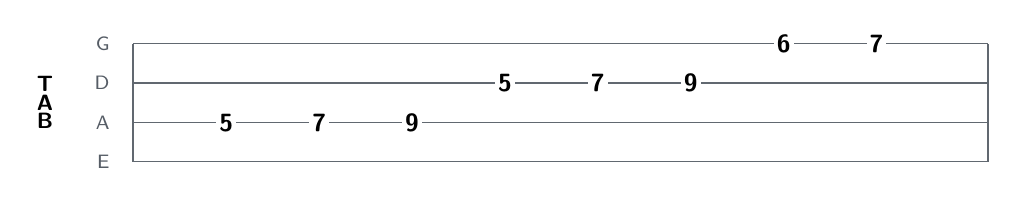
\begin{tikzpicture}[x=1.18cm,y=0.50cm]
\node[font=\sffamily\bfseries\footnotesize,align=center] at (-0.95,1.50) {T\\[-1mm]A\\[-1mm]B};
\foreach \y/\s in {3/G,2/D,1/A,0/E} {
  \draw[Ink!70,line width=0.55pt] (0,\y) -- (9.2,\y);
  \node[anchor=east,font=\sffamily\scriptsize,text=Ink!75] at (-0.15,\y) {\s};
}
\draw[Ink!70,line width=0.7pt] (0,0) -- (0,3);
\draw[Ink!70,line width=0.7pt] (9.2,0) -- (9.2,3);
\TabNum{1}{1}{5}
\TabNum{2}{1}{7}
\TabNum{3}{1}{9}
\TabNum{4}{2}{5}
\TabNum{5}{2}{7}
\TabNum{6}{2}{9}
\TabNum{7}{3}{6}
\TabNum{8}{3}{7}
\end{tikzpicture}
\endgroup
\end{center}

\begin{tabularx}{\textwidth}{>{\bfseries\sffamily}p{3.0cm}Y}
Signature sound & Natural 3 and natural 7 \\
Harmonic fit & Major keys; major and major-7 chords \\
Overall colour & Stable, bright, resolved \\
Comparison & Reference scale for all interval formulas. \\
\end{tabularx}
\clearpage
\section{Natural minor (Aeolian)}\label{scale:natural-minor}
\begin{tabularx}{\textwidth}{>{\bfseries\sffamily}p{2.8cm}Y}
Formula & 1 2 $\flat3$ 4 5 $\flat6$ $\flat7$ \\
Step pattern & W -- H -- W -- W -- H -- W -- W \\
D example & D--E--F--G--A--B$\flat$--C--D \\
\end{tabularx}
\begin{center}
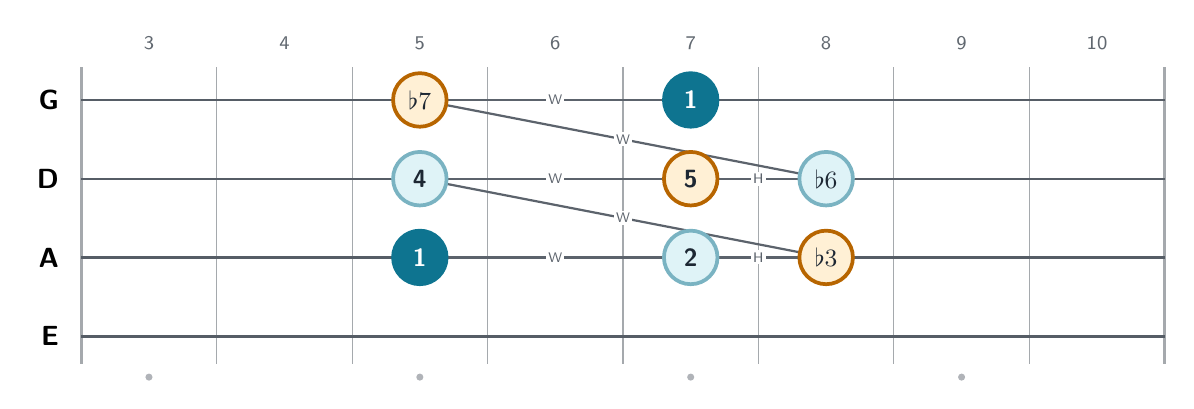
\begin{tikzpicture}[x=1cm,y=1cm,>=stealth]
\node[font=\sffamily\scriptsize,text=Ink!70] at (0.860,4.22) {3};
\node[font=\sffamily\scriptsize,text=Ink!70] at (2.580,4.22) {4};
\node[font=\sffamily\scriptsize,text=Ink!70] at (4.300,4.22) {5};
\node[font=\sffamily\scriptsize,text=Ink!70] at (6.020,4.22) {6};
\node[font=\sffamily\scriptsize,text=Ink!70] at (7.740,4.22) {7};
\node[font=\sffamily\scriptsize,text=Ink!70] at (9.460,4.22) {8};
\node[font=\sffamily\scriptsize,text=Ink!70] at (11.180,4.22) {9};
\node[font=\sffamily\scriptsize,text=Ink!70] at (12.900,4.22) {10};
\draw[Ink!40,line width=1.0pt] (0.000,0.15) -- (0.000,3.92);
\draw[Ink!40,line width=0.45pt] (1.720,0.15) -- (1.720,3.92);
\draw[Ink!40,line width=0.45pt] (3.440,0.15) -- (3.440,3.92);
\draw[Ink!40,line width=0.45pt] (5.160,0.15) -- (5.160,3.92);
\draw[Ink!40,line width=0.45pt] (6.880,0.15) -- (6.880,3.92);
\draw[Ink!40,line width=0.45pt] (8.600,0.15) -- (8.600,3.92);
\draw[Ink!40,line width=0.45pt] (10.320,0.15) -- (10.320,3.92);
\draw[Ink!40,line width=0.45pt] (12.040,0.15) -- (12.040,3.92);
\draw[Ink!40,line width=1.0pt] (13.760,0.15) -- (13.760,3.92);
\node[anchor=east,font=\sffamily\bfseries] at (-0.16,3.50) {G};
\draw[Ink!75,line width=0.45pt] (0,3.50) -- (13.760,3.50);
\node[anchor=east,font=\sffamily\bfseries] at (-0.16,2.50) {D};
\draw[Ink!75,line width=0.6pt] (0,2.50) -- (13.760,2.50);
\node[anchor=east,font=\sffamily\bfseries] at (-0.16,1.50) {A};
\draw[Ink!75,line width=0.8pt] (0,1.50) -- (13.760,1.50);
\node[anchor=east,font=\sffamily\bfseries] at (-0.16,0.50) {E};
\draw[Ink!75,line width=1.0pt] (0,0.50) -- (13.760,0.50);
\fill[Ink!35] (0.860,-0.02) circle (0.045);
\fill[Ink!35] (4.300,-0.02) circle (0.045);
\fill[Ink!35] (7.740,-0.02) circle (0.045);
\fill[Ink!35] (11.180,-0.02) circle (0.045);
\draw[->,Ink!72,line width=0.8pt] (4.300,1.500) -- node[midway,fill=white,inner sep=0.8pt,font=\sffamily\tiny] {W} (7.740,1.500);
\draw[->,Ink!72,line width=0.8pt] (7.740,1.500) -- node[midway,fill=white,inner sep=0.8pt,font=\sffamily\tiny] {H} (9.460,1.500);
\draw[->,Ink!72,line width=0.8pt] (9.460,1.500) -- node[midway,fill=white,inner sep=0.8pt,font=\sffamily\tiny] {W} (4.300,2.500);
\draw[->,Ink!72,line width=0.8pt] (4.300,2.500) -- node[midway,fill=white,inner sep=0.8pt,font=\sffamily\tiny] {W} (7.740,2.500);
\draw[->,Ink!72,line width=0.8pt] (7.740,2.500) -- node[midway,fill=white,inner sep=0.8pt,font=\sffamily\tiny] {H} (9.460,2.500);
\draw[->,Ink!72,line width=0.8pt] (9.460,2.500) -- node[midway,fill=white,inner sep=0.8pt,font=\sffamily\tiny] {W} (4.300,3.500);
\draw[->,Ink!72,line width=0.8pt] (4.300,3.500) -- node[midway,fill=white,inner sep=0.8pt,font=\sffamily\tiny] {W} (7.740,3.500);
\node[circle,minimum size=0.68cm,inner sep=0pt,fill=ChordLight,draw=Chord,line width=1.35pt,font=\sffamily\bfseries\small,text=Ink] at (4.300,3.500) {$\flat7$};
\node[circle,minimum size=0.68cm,inner sep=0pt,fill=Accent,draw=Accent,line width=1.35pt,font=\sffamily\bfseries\small,text=white] at (7.740,3.500) {1};
\node[circle,minimum size=0.68cm,inner sep=0pt,fill=AccentLight,draw=Accent!55,line width=1.35pt,font=\sffamily\bfseries\small,text=Ink] at (4.300,2.500) {4};
\node[circle,minimum size=0.68cm,inner sep=0pt,fill=ChordLight,draw=Chord,line width=1.35pt,font=\sffamily\bfseries\small,text=Ink] at (7.740,2.500) {5};
\node[circle,minimum size=0.68cm,inner sep=0pt,fill=AccentLight,draw=Accent!55,line width=1.35pt,font=\sffamily\bfseries\small,text=Ink] at (9.460,2.500) {$\flat6$};
\node[circle,minimum size=0.68cm,inner sep=0pt,fill=Accent,draw=Accent,line width=1.35pt,font=\sffamily\bfseries\small,text=white] at (4.300,1.500) {1};
\node[circle,minimum size=0.68cm,inner sep=0pt,fill=AccentLight,draw=Accent!55,line width=1.35pt,font=\sffamily\bfseries\small,text=Ink] at (7.740,1.500) {2};
\node[circle,minimum size=0.68cm,inner sep=0pt,fill=ChordLight,draw=Chord,line width=1.35pt,font=\sffamily\bfseries\small,text=Ink] at (9.460,1.500) {$\flat3$};
\end{tikzpicture}
\end{center}
\vspace{1mm}
\begin{center}
\begingroup
\setlength{\parindent}{0pt}
\begin{minipage}{0.82\textwidth}
{\sffamily\bfseries\small Standard notation}\par\vspace{-1mm}
\begin{music}
\instrumentnumber{1}
\setstaffs1{1}
\setclef1{\bass}
\nobarnumbers
\nostartrule
\startextract
\NOtes\qu K\qu L\qu M\qu N\qu a\qu{_b}\qu c\qu d\en
\zendextract
\end{music}
\end{minipage}
\vspace{-1mm}

{\sffamily\bfseries\small Bass TAB}\par\vspace{1mm}
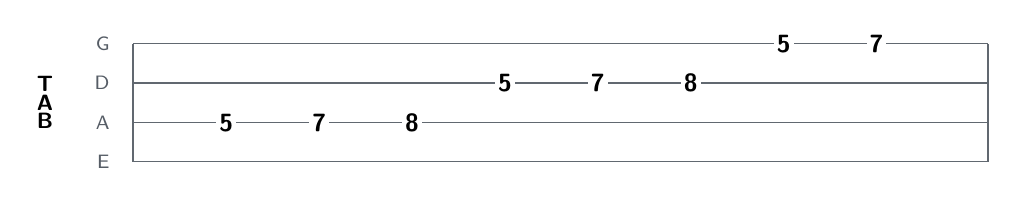
\begin{tikzpicture}[x=1.18cm,y=0.50cm]
\node[font=\sffamily\bfseries\footnotesize,align=center] at (-0.95,1.50) {T\\[-1mm]A\\[-1mm]B};
\foreach \y/\s in {3/G,2/D,1/A,0/E} {
  \draw[Ink!70,line width=0.55pt] (0,\y) -- (9.2,\y);
  \node[anchor=east,font=\sffamily\scriptsize,text=Ink!75] at (-0.15,\y) {\s};
}
\draw[Ink!70,line width=0.7pt] (0,0) -- (0,3);
\draw[Ink!70,line width=0.7pt] (9.2,0) -- (9.2,3);
\TabNum{1}{1}{5}
\TabNum{2}{1}{7}
\TabNum{3}{1}{8}
\TabNum{4}{2}{5}
\TabNum{5}{2}{7}
\TabNum{6}{2}{8}
\TabNum{7}{3}{5}
\TabNum{8}{3}{7}
\end{tikzpicture}
\endgroup
\end{center}

\begin{tabularx}{\textwidth}{>{\bfseries\sffamily}p{3.0cm}Y}
Signature sound & $\flat3$, $\flat6$, $\flat7$ \\
Harmonic fit & Minor keys; minor and minor-7 chords when the harmony contains $\flat6$ \\
Overall colour & Dark, settled minor sound \\
Comparison & Relative minor of F major; parallel minor of D major. \\
\end{tabularx}
\clearpage
\section{Dorian}\label{scale:dorian}
\begin{tabularx}{\textwidth}{>{\bfseries\sffamily}p{2.8cm}Y}
Formula & 1 2 $\flat3$ 4 5 6 $\flat7$ \\
Step pattern & W -- H -- W -- W -- W -- H -- W \\
D example & D--E--F--G--A--B--C--D \\
\end{tabularx}
\begin{center}
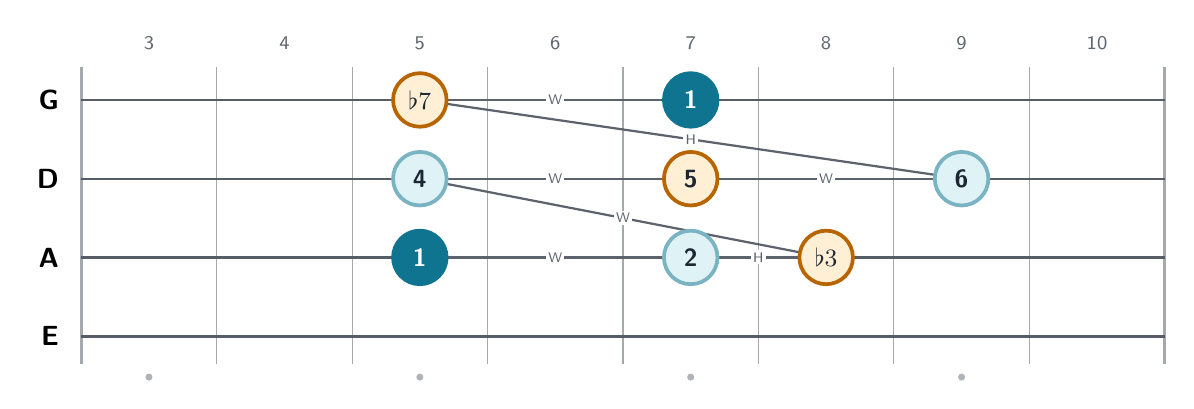
\begin{tikzpicture}[x=1cm,y=1cm,>=stealth]
\node[font=\sffamily\scriptsize,text=Ink!70] at (0.860,4.22) {3};
\node[font=\sffamily\scriptsize,text=Ink!70] at (2.580,4.22) {4};
\node[font=\sffamily\scriptsize,text=Ink!70] at (4.300,4.22) {5};
\node[font=\sffamily\scriptsize,text=Ink!70] at (6.020,4.22) {6};
\node[font=\sffamily\scriptsize,text=Ink!70] at (7.740,4.22) {7};
\node[font=\sffamily\scriptsize,text=Ink!70] at (9.460,4.22) {8};
\node[font=\sffamily\scriptsize,text=Ink!70] at (11.180,4.22) {9};
\node[font=\sffamily\scriptsize,text=Ink!70] at (12.900,4.22) {10};
\draw[Ink!40,line width=1.0pt] (0.000,0.15) -- (0.000,3.92);
\draw[Ink!40,line width=0.45pt] (1.720,0.15) -- (1.720,3.92);
\draw[Ink!40,line width=0.45pt] (3.440,0.15) -- (3.440,3.92);
\draw[Ink!40,line width=0.45pt] (5.160,0.15) -- (5.160,3.92);
\draw[Ink!40,line width=0.45pt] (6.880,0.15) -- (6.880,3.92);
\draw[Ink!40,line width=0.45pt] (8.600,0.15) -- (8.600,3.92);
\draw[Ink!40,line width=0.45pt] (10.320,0.15) -- (10.320,3.92);
\draw[Ink!40,line width=0.45pt] (12.040,0.15) -- (12.040,3.92);
\draw[Ink!40,line width=1.0pt] (13.760,0.15) -- (13.760,3.92);
\node[anchor=east,font=\sffamily\bfseries] at (-0.16,3.50) {G};
\draw[Ink!75,line width=0.45pt] (0,3.50) -- (13.760,3.50);
\node[anchor=east,font=\sffamily\bfseries] at (-0.16,2.50) {D};
\draw[Ink!75,line width=0.6pt] (0,2.50) -- (13.760,2.50);
\node[anchor=east,font=\sffamily\bfseries] at (-0.16,1.50) {A};
\draw[Ink!75,line width=0.8pt] (0,1.50) -- (13.760,1.50);
\node[anchor=east,font=\sffamily\bfseries] at (-0.16,0.50) {E};
\draw[Ink!75,line width=1.0pt] (0,0.50) -- (13.760,0.50);
\fill[Ink!35] (0.860,-0.02) circle (0.045);
\fill[Ink!35] (4.300,-0.02) circle (0.045);
\fill[Ink!35] (7.740,-0.02) circle (0.045);
\fill[Ink!35] (11.180,-0.02) circle (0.045);
\draw[->,Ink!72,line width=0.8pt] (4.300,1.500) -- node[midway,fill=white,inner sep=0.8pt,font=\sffamily\tiny] {W} (7.740,1.500);
\draw[->,Ink!72,line width=0.8pt] (7.740,1.500) -- node[midway,fill=white,inner sep=0.8pt,font=\sffamily\tiny] {H} (9.460,1.500);
\draw[->,Ink!72,line width=0.8pt] (9.460,1.500) -- node[midway,fill=white,inner sep=0.8pt,font=\sffamily\tiny] {W} (4.300,2.500);
\draw[->,Ink!72,line width=0.8pt] (4.300,2.500) -- node[midway,fill=white,inner sep=0.8pt,font=\sffamily\tiny] {W} (7.740,2.500);
\draw[->,Ink!72,line width=0.8pt] (7.740,2.500) -- node[midway,fill=white,inner sep=0.8pt,font=\sffamily\tiny] {W} (11.180,2.500);
\draw[->,Ink!72,line width=0.8pt] (11.180,2.500) -- node[midway,fill=white,inner sep=0.8pt,font=\sffamily\tiny] {H} (4.300,3.500);
\draw[->,Ink!72,line width=0.8pt] (4.300,3.500) -- node[midway,fill=white,inner sep=0.8pt,font=\sffamily\tiny] {W} (7.740,3.500);
\node[circle,minimum size=0.68cm,inner sep=0pt,fill=ChordLight,draw=Chord,line width=1.35pt,font=\sffamily\bfseries\small,text=Ink] at (4.300,3.500) {$\flat7$};
\node[circle,minimum size=0.68cm,inner sep=0pt,fill=Accent,draw=Accent,line width=1.35pt,font=\sffamily\bfseries\small,text=white] at (7.740,3.500) {1};
\node[circle,minimum size=0.68cm,inner sep=0pt,fill=AccentLight,draw=Accent!55,line width=1.35pt,font=\sffamily\bfseries\small,text=Ink] at (4.300,2.500) {4};
\node[circle,minimum size=0.68cm,inner sep=0pt,fill=ChordLight,draw=Chord,line width=1.35pt,font=\sffamily\bfseries\small,text=Ink] at (7.740,2.500) {5};
\node[circle,minimum size=0.68cm,inner sep=0pt,fill=AccentLight,draw=Accent!55,line width=1.35pt,font=\sffamily\bfseries\small,text=Ink] at (11.180,2.500) {6};
\node[circle,minimum size=0.68cm,inner sep=0pt,fill=Accent,draw=Accent,line width=1.35pt,font=\sffamily\bfseries\small,text=white] at (4.300,1.500) {1};
\node[circle,minimum size=0.68cm,inner sep=0pt,fill=AccentLight,draw=Accent!55,line width=1.35pt,font=\sffamily\bfseries\small,text=Ink] at (7.740,1.500) {2};
\node[circle,minimum size=0.68cm,inner sep=0pt,fill=ChordLight,draw=Chord,line width=1.35pt,font=\sffamily\bfseries\small,text=Ink] at (9.460,1.500) {$\flat3$};
\end{tikzpicture}
\end{center}
\vspace{1mm}
\begin{center}
\begingroup
\setlength{\parindent}{0pt}
\begin{minipage}{0.82\textwidth}
{\sffamily\bfseries\small Standard notation}\par\vspace{-1mm}
\begin{music}
\instrumentnumber{1}
\setstaffs1{1}
\setclef1{\bass}
\nobarnumbers
\nostartrule
\startextract
\NOtes\qu K\qu L\qu M\qu N\qu a\qu b\qu c\qu d\en
\zendextract
\end{music}
\end{minipage}
\vspace{-1mm}

{\sffamily\bfseries\small Bass TAB}\par\vspace{1mm}
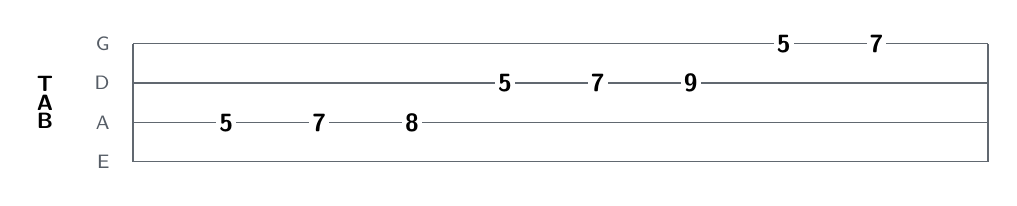
\begin{tikzpicture}[x=1.18cm,y=0.50cm]
\node[font=\sffamily\bfseries\footnotesize,align=center] at (-0.95,1.50) {T\\[-1mm]A\\[-1mm]B};
\foreach \y/\s in {3/G,2/D,1/A,0/E} {
  \draw[Ink!70,line width=0.55pt] (0,\y) -- (9.2,\y);
  \node[anchor=east,font=\sffamily\scriptsize,text=Ink!75] at (-0.15,\y) {\s};
}
\draw[Ink!70,line width=0.7pt] (0,0) -- (0,3);
\draw[Ink!70,line width=0.7pt] (9.2,0) -- (9.2,3);
\TabNum{1}{1}{5}
\TabNum{2}{1}{7}
\TabNum{3}{1}{8}
\TabNum{4}{2}{5}
\TabNum{5}{2}{7}
\TabNum{6}{2}{9}
\TabNum{7}{3}{5}
\TabNum{8}{3}{7}
\end{tikzpicture}
\endgroup
\end{center}

\begin{tabularx}{\textwidth}{>{\bfseries\sffamily}p{3.0cm}Y}
Signature sound & Natural 6 over a minor chord \\
Harmonic fit & Minor-7 grooves, funk, modal jazz, Latin harmony \\
Overall colour & Minor with a brighter, more open sixth \\
Comparison & Natural minor with $\flat6$ raised to 6. \\
\end{tabularx}
\clearpage
\section{Phrygian}
\begin{tabularx}{\textwidth}{>{\bfseries\sffamily}p{2.8cm}Y}
Formula & 1 $\flat2$ $\flat3$ 4 5 $\flat6$ $\flat7$ \\
Step pattern & H -- W -- W -- W -- H -- W -- W \\
D example & D--E$\flat$--F--G--A--B$\flat$--C--D \\
\end{tabularx}
\begin{center}
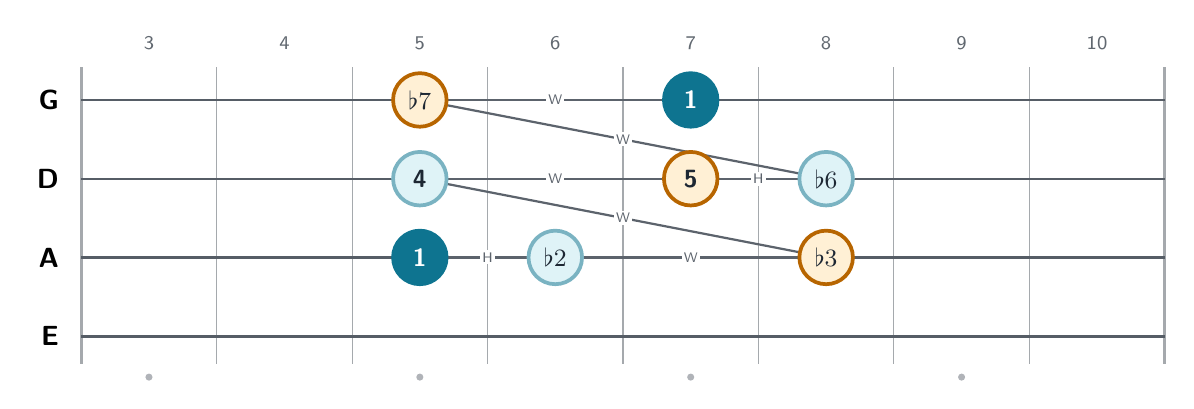
\begin{tikzpicture}[x=1cm,y=1cm,>=stealth]
\node[font=\sffamily\scriptsize,text=Ink!70] at (0.860,4.22) {3};
\node[font=\sffamily\scriptsize,text=Ink!70] at (2.580,4.22) {4};
\node[font=\sffamily\scriptsize,text=Ink!70] at (4.300,4.22) {5};
\node[font=\sffamily\scriptsize,text=Ink!70] at (6.020,4.22) {6};
\node[font=\sffamily\scriptsize,text=Ink!70] at (7.740,4.22) {7};
\node[font=\sffamily\scriptsize,text=Ink!70] at (9.460,4.22) {8};
\node[font=\sffamily\scriptsize,text=Ink!70] at (11.180,4.22) {9};
\node[font=\sffamily\scriptsize,text=Ink!70] at (12.900,4.22) {10};
\draw[Ink!40,line width=1.0pt] (0.000,0.15) -- (0.000,3.92);
\draw[Ink!40,line width=0.45pt] (1.720,0.15) -- (1.720,3.92);
\draw[Ink!40,line width=0.45pt] (3.440,0.15) -- (3.440,3.92);
\draw[Ink!40,line width=0.45pt] (5.160,0.15) -- (5.160,3.92);
\draw[Ink!40,line width=0.45pt] (6.880,0.15) -- (6.880,3.92);
\draw[Ink!40,line width=0.45pt] (8.600,0.15) -- (8.600,3.92);
\draw[Ink!40,line width=0.45pt] (10.320,0.15) -- (10.320,3.92);
\draw[Ink!40,line width=0.45pt] (12.040,0.15) -- (12.040,3.92);
\draw[Ink!40,line width=1.0pt] (13.760,0.15) -- (13.760,3.92);
\node[anchor=east,font=\sffamily\bfseries] at (-0.16,3.50) {G};
\draw[Ink!75,line width=0.45pt] (0,3.50) -- (13.760,3.50);
\node[anchor=east,font=\sffamily\bfseries] at (-0.16,2.50) {D};
\draw[Ink!75,line width=0.6pt] (0,2.50) -- (13.760,2.50);
\node[anchor=east,font=\sffamily\bfseries] at (-0.16,1.50) {A};
\draw[Ink!75,line width=0.8pt] (0,1.50) -- (13.760,1.50);
\node[anchor=east,font=\sffamily\bfseries] at (-0.16,0.50) {E};
\draw[Ink!75,line width=1.0pt] (0,0.50) -- (13.760,0.50);
\fill[Ink!35] (0.860,-0.02) circle (0.045);
\fill[Ink!35] (4.300,-0.02) circle (0.045);
\fill[Ink!35] (7.740,-0.02) circle (0.045);
\fill[Ink!35] (11.180,-0.02) circle (0.045);
\draw[->,Ink!72,line width=0.8pt] (4.300,1.500) -- node[midway,fill=white,inner sep=0.8pt,font=\sffamily\tiny] {H} (6.020,1.500);
\draw[->,Ink!72,line width=0.8pt] (6.020,1.500) -- node[midway,fill=white,inner sep=0.8pt,font=\sffamily\tiny] {W} (9.460,1.500);
\draw[->,Ink!72,line width=0.8pt] (9.460,1.500) -- node[midway,fill=white,inner sep=0.8pt,font=\sffamily\tiny] {W} (4.300,2.500);
\draw[->,Ink!72,line width=0.8pt] (4.300,2.500) -- node[midway,fill=white,inner sep=0.8pt,font=\sffamily\tiny] {W} (7.740,2.500);
\draw[->,Ink!72,line width=0.8pt] (7.740,2.500) -- node[midway,fill=white,inner sep=0.8pt,font=\sffamily\tiny] {H} (9.460,2.500);
\draw[->,Ink!72,line width=0.8pt] (9.460,2.500) -- node[midway,fill=white,inner sep=0.8pt,font=\sffamily\tiny] {W} (4.300,3.500);
\draw[->,Ink!72,line width=0.8pt] (4.300,3.500) -- node[midway,fill=white,inner sep=0.8pt,font=\sffamily\tiny] {W} (7.740,3.500);
\node[circle,minimum size=0.68cm,inner sep=0pt,fill=ChordLight,draw=Chord,line width=1.35pt,font=\sffamily\bfseries\small,text=Ink] at (4.300,3.500) {$\flat7$};
\node[circle,minimum size=0.68cm,inner sep=0pt,fill=Accent,draw=Accent,line width=1.35pt,font=\sffamily\bfseries\small,text=white] at (7.740,3.500) {1};
\node[circle,minimum size=0.68cm,inner sep=0pt,fill=AccentLight,draw=Accent!55,line width=1.35pt,font=\sffamily\bfseries\small,text=Ink] at (4.300,2.500) {4};
\node[circle,minimum size=0.68cm,inner sep=0pt,fill=ChordLight,draw=Chord,line width=1.35pt,font=\sffamily\bfseries\small,text=Ink] at (7.740,2.500) {5};
\node[circle,minimum size=0.68cm,inner sep=0pt,fill=AccentLight,draw=Accent!55,line width=1.35pt,font=\sffamily\bfseries\small,text=Ink] at (9.460,2.500) {$\flat6$};
\node[circle,minimum size=0.68cm,inner sep=0pt,fill=Accent,draw=Accent,line width=1.35pt,font=\sffamily\bfseries\small,text=white] at (4.300,1.500) {1};
\node[circle,minimum size=0.68cm,inner sep=0pt,fill=AccentLight,draw=Accent!55,line width=1.35pt,font=\sffamily\bfseries\small,text=Ink] at (6.020,1.500) {$\flat2$};
\node[circle,minimum size=0.68cm,inner sep=0pt,fill=ChordLight,draw=Chord,line width=1.35pt,font=\sffamily\bfseries\small,text=Ink] at (9.460,1.500) {$\flat3$};
\end{tikzpicture}
\end{center}
\vspace{1mm}
\begin{center}
\begingroup
\setlength{\parindent}{0pt}
\begin{minipage}{0.82\textwidth}
{\sffamily\bfseries\small Standard notation}\par\vspace{-1mm}
\begin{music}
\instrumentnumber{1}
\setstaffs1{1}
\setclef1{\bass}
\nobarnumbers
\nostartrule
\startextract
\NOtes\qu K\qu{_L}\qu M\qu N\qu a\qu{_b}\qu c\qu d\en
\zendextract
\end{music}
\end{minipage}
\vspace{-1mm}

{\sffamily\bfseries\small Bass TAB}\par\vspace{1mm}
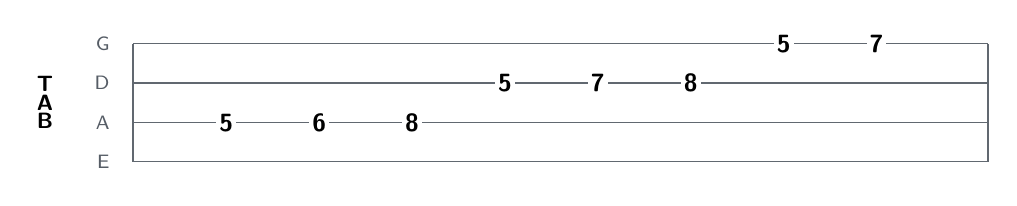
\begin{tikzpicture}[x=1.18cm,y=0.50cm]
\node[font=\sffamily\bfseries\footnotesize,align=center] at (-0.95,1.50) {T\\[-1mm]A\\[-1mm]B};
\foreach \y/\s in {3/G,2/D,1/A,0/E} {
  \draw[Ink!70,line width=0.55pt] (0,\y) -- (9.2,\y);
  \node[anchor=east,font=\sffamily\scriptsize,text=Ink!75] at (-0.15,\y) {\s};
}
\draw[Ink!70,line width=0.7pt] (0,0) -- (0,3);
\draw[Ink!70,line width=0.7pt] (9.2,0) -- (9.2,3);
\TabNum{1}{1}{5}
\TabNum{2}{1}{6}
\TabNum{3}{1}{8}
\TabNum{4}{2}{5}
\TabNum{5}{2}{7}
\TabNum{6}{2}{8}
\TabNum{7}{3}{5}
\TabNum{8}{3}{7}
\end{tikzpicture}
\endgroup
\end{center}

\begin{tabularx}{\textwidth}{>{\bfseries\sffamily}p{3.0cm}Y}
Signature sound & $\flat2$ \\
Harmonic fit & Minor chords with a strong lowered-second colour; Spanish and metal contexts \\
Overall colour & Dark and compressed around the root \\
Comparison & Natural minor with 2 lowered to $\flat2$. \\
\end{tabularx}
\clearpage
\section{Lydian}
\begin{tabularx}{\textwidth}{>{\bfseries\sffamily}p{2.8cm}Y}
Formula & 1 2 3 $\sharp4$ 5 6 7 \\
Step pattern & W -- W -- W -- H -- W -- W -- H \\
D example & D--E--F\#--G\#--A--B--C\#--D \\
\end{tabularx}
\begin{center}
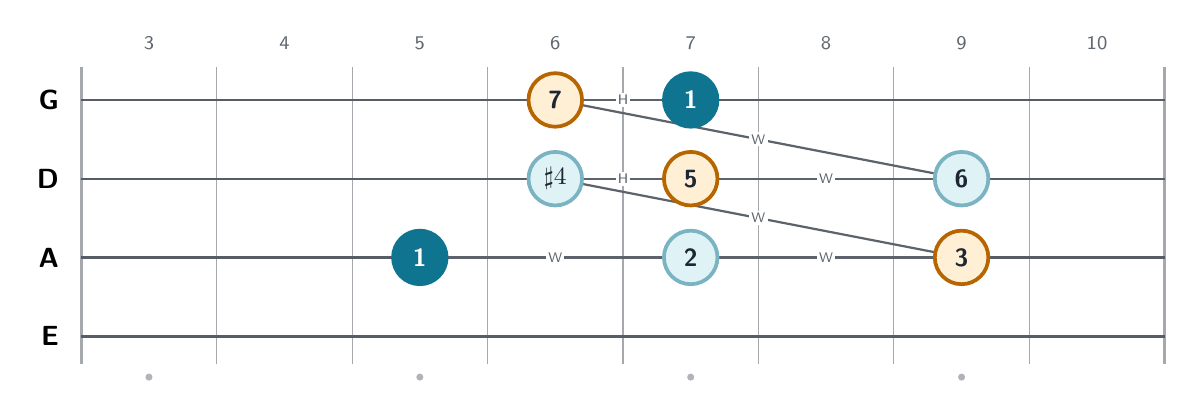
\begin{tikzpicture}[x=1cm,y=1cm,>=stealth]
\node[font=\sffamily\scriptsize,text=Ink!70] at (0.860,4.22) {3};
\node[font=\sffamily\scriptsize,text=Ink!70] at (2.580,4.22) {4};
\node[font=\sffamily\scriptsize,text=Ink!70] at (4.300,4.22) {5};
\node[font=\sffamily\scriptsize,text=Ink!70] at (6.020,4.22) {6};
\node[font=\sffamily\scriptsize,text=Ink!70] at (7.740,4.22) {7};
\node[font=\sffamily\scriptsize,text=Ink!70] at (9.460,4.22) {8};
\node[font=\sffamily\scriptsize,text=Ink!70] at (11.180,4.22) {9};
\node[font=\sffamily\scriptsize,text=Ink!70] at (12.900,4.22) {10};
\draw[Ink!40,line width=1.0pt] (0.000,0.15) -- (0.000,3.92);
\draw[Ink!40,line width=0.45pt] (1.720,0.15) -- (1.720,3.92);
\draw[Ink!40,line width=0.45pt] (3.440,0.15) -- (3.440,3.92);
\draw[Ink!40,line width=0.45pt] (5.160,0.15) -- (5.160,3.92);
\draw[Ink!40,line width=0.45pt] (6.880,0.15) -- (6.880,3.92);
\draw[Ink!40,line width=0.45pt] (8.600,0.15) -- (8.600,3.92);
\draw[Ink!40,line width=0.45pt] (10.320,0.15) -- (10.320,3.92);
\draw[Ink!40,line width=0.45pt] (12.040,0.15) -- (12.040,3.92);
\draw[Ink!40,line width=1.0pt] (13.760,0.15) -- (13.760,3.92);
\node[anchor=east,font=\sffamily\bfseries] at (-0.16,3.50) {G};
\draw[Ink!75,line width=0.45pt] (0,3.50) -- (13.760,3.50);
\node[anchor=east,font=\sffamily\bfseries] at (-0.16,2.50) {D};
\draw[Ink!75,line width=0.6pt] (0,2.50) -- (13.760,2.50);
\node[anchor=east,font=\sffamily\bfseries] at (-0.16,1.50) {A};
\draw[Ink!75,line width=0.8pt] (0,1.50) -- (13.760,1.50);
\node[anchor=east,font=\sffamily\bfseries] at (-0.16,0.50) {E};
\draw[Ink!75,line width=1.0pt] (0,0.50) -- (13.760,0.50);
\fill[Ink!35] (0.860,-0.02) circle (0.045);
\fill[Ink!35] (4.300,-0.02) circle (0.045);
\fill[Ink!35] (7.740,-0.02) circle (0.045);
\fill[Ink!35] (11.180,-0.02) circle (0.045);
\draw[->,Ink!72,line width=0.8pt] (4.300,1.500) -- node[midway,fill=white,inner sep=0.8pt,font=\sffamily\tiny] {W} (7.740,1.500);
\draw[->,Ink!72,line width=0.8pt] (7.740,1.500) -- node[midway,fill=white,inner sep=0.8pt,font=\sffamily\tiny] {W} (11.180,1.500);
\draw[->,Ink!72,line width=0.8pt] (11.180,1.500) -- node[midway,fill=white,inner sep=0.8pt,font=\sffamily\tiny] {W} (6.020,2.500);
\draw[->,Ink!72,line width=0.8pt] (6.020,2.500) -- node[midway,fill=white,inner sep=0.8pt,font=\sffamily\tiny] {H} (7.740,2.500);
\draw[->,Ink!72,line width=0.8pt] (7.740,2.500) -- node[midway,fill=white,inner sep=0.8pt,font=\sffamily\tiny] {W} (11.180,2.500);
\draw[->,Ink!72,line width=0.8pt] (11.180,2.500) -- node[midway,fill=white,inner sep=0.8pt,font=\sffamily\tiny] {W} (6.020,3.500);
\draw[->,Ink!72,line width=0.8pt] (6.020,3.500) -- node[midway,fill=white,inner sep=0.8pt,font=\sffamily\tiny] {H} (7.740,3.500);
\node[circle,minimum size=0.68cm,inner sep=0pt,fill=ChordLight,draw=Chord,line width=1.35pt,font=\sffamily\bfseries\small,text=Ink] at (6.020,3.500) {7};
\node[circle,minimum size=0.68cm,inner sep=0pt,fill=Accent,draw=Accent,line width=1.35pt,font=\sffamily\bfseries\small,text=white] at (7.740,3.500) {1};
\node[circle,minimum size=0.68cm,inner sep=0pt,fill=AccentLight,draw=Accent!55,line width=1.35pt,font=\sffamily\bfseries\small,text=Ink] at (6.020,2.500) {$\sharp4$};
\node[circle,minimum size=0.68cm,inner sep=0pt,fill=ChordLight,draw=Chord,line width=1.35pt,font=\sffamily\bfseries\small,text=Ink] at (7.740,2.500) {5};
\node[circle,minimum size=0.68cm,inner sep=0pt,fill=AccentLight,draw=Accent!55,line width=1.35pt,font=\sffamily\bfseries\small,text=Ink] at (11.180,2.500) {6};
\node[circle,minimum size=0.68cm,inner sep=0pt,fill=Accent,draw=Accent,line width=1.35pt,font=\sffamily\bfseries\small,text=white] at (4.300,1.500) {1};
\node[circle,minimum size=0.68cm,inner sep=0pt,fill=AccentLight,draw=Accent!55,line width=1.35pt,font=\sffamily\bfseries\small,text=Ink] at (7.740,1.500) {2};
\node[circle,minimum size=0.68cm,inner sep=0pt,fill=ChordLight,draw=Chord,line width=1.35pt,font=\sffamily\bfseries\small,text=Ink] at (11.180,1.500) {3};
\end{tikzpicture}
\end{center}
\vspace{1mm}
\begin{center}
\begingroup
\setlength{\parindent}{0pt}
\begin{minipage}{0.82\textwidth}
{\sffamily\bfseries\small Standard notation}\par\vspace{-1mm}
\begin{music}
\instrumentnumber{1}
\setstaffs1{1}
\setclef1{\bass}
\nobarnumbers
\nostartrule
\startextract
\NOtes\qu K\qu L\qu{^M}\qu{^N}\qu a\qu b\qu{^c}\qu d\en
\zendextract
\end{music}
\end{minipage}
\vspace{-1mm}

{\sffamily\bfseries\small Bass TAB}\par\vspace{1mm}
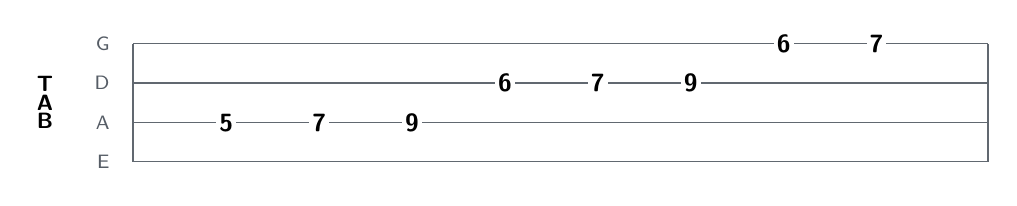
\begin{tikzpicture}[x=1.18cm,y=0.50cm]
\node[font=\sffamily\bfseries\footnotesize,align=center] at (-0.95,1.50) {T\\[-1mm]A\\[-1mm]B};
\foreach \y/\s in {3/G,2/D,1/A,0/E} {
  \draw[Ink!70,line width=0.55pt] (0,\y) -- (9.2,\y);
  \node[anchor=east,font=\sffamily\scriptsize,text=Ink!75] at (-0.15,\y) {\s};
}
\draw[Ink!70,line width=0.7pt] (0,0) -- (0,3);
\draw[Ink!70,line width=0.7pt] (9.2,0) -- (9.2,3);
\TabNum{1}{1}{5}
\TabNum{2}{1}{7}
\TabNum{3}{1}{9}
\TabNum{4}{2}{6}
\TabNum{5}{2}{7}
\TabNum{6}{2}{9}
\TabNum{7}{3}{6}
\TabNum{8}{3}{7}
\end{tikzpicture}
\endgroup
\end{center}

\begin{tabularx}{\textwidth}{>{\bfseries\sffamily}p{3.0cm}Y}
Signature sound & $\sharp4$ \\
Harmonic fit & Major chords with $\sharp11$; sustained major harmony \\
Overall colour & Bright, floating, less final than Ionian \\
Comparison & Major scale with 4 raised to $\sharp4$. \\
\end{tabularx}
\clearpage
\section{Mixolydian}\label{scale:mixolydian}
\begin{tabularx}{\textwidth}{>{\bfseries\sffamily}p{2.8cm}Y}
Formula & 1 2 3 4 5 6 $\flat7$ \\
Step pattern & W -- W -- H -- W -- W -- H -- W \\
D example & D--E--F\#--G--A--B--C--D \\
\end{tabularx}
\begin{center}
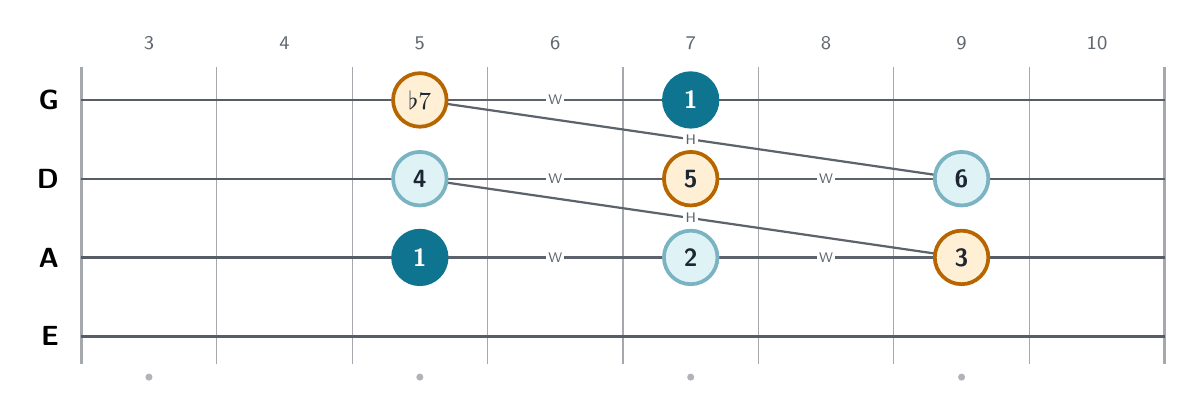
\begin{tikzpicture}[x=1cm,y=1cm,>=stealth]
\node[font=\sffamily\scriptsize,text=Ink!70] at (0.860,4.22) {3};
\node[font=\sffamily\scriptsize,text=Ink!70] at (2.580,4.22) {4};
\node[font=\sffamily\scriptsize,text=Ink!70] at (4.300,4.22) {5};
\node[font=\sffamily\scriptsize,text=Ink!70] at (6.020,4.22) {6};
\node[font=\sffamily\scriptsize,text=Ink!70] at (7.740,4.22) {7};
\node[font=\sffamily\scriptsize,text=Ink!70] at (9.460,4.22) {8};
\node[font=\sffamily\scriptsize,text=Ink!70] at (11.180,4.22) {9};
\node[font=\sffamily\scriptsize,text=Ink!70] at (12.900,4.22) {10};
\draw[Ink!40,line width=1.0pt] (0.000,0.15) -- (0.000,3.92);
\draw[Ink!40,line width=0.45pt] (1.720,0.15) -- (1.720,3.92);
\draw[Ink!40,line width=0.45pt] (3.440,0.15) -- (3.440,3.92);
\draw[Ink!40,line width=0.45pt] (5.160,0.15) -- (5.160,3.92);
\draw[Ink!40,line width=0.45pt] (6.880,0.15) -- (6.880,3.92);
\draw[Ink!40,line width=0.45pt] (8.600,0.15) -- (8.600,3.92);
\draw[Ink!40,line width=0.45pt] (10.320,0.15) -- (10.320,3.92);
\draw[Ink!40,line width=0.45pt] (12.040,0.15) -- (12.040,3.92);
\draw[Ink!40,line width=1.0pt] (13.760,0.15) -- (13.760,3.92);
\node[anchor=east,font=\sffamily\bfseries] at (-0.16,3.50) {G};
\draw[Ink!75,line width=0.45pt] (0,3.50) -- (13.760,3.50);
\node[anchor=east,font=\sffamily\bfseries] at (-0.16,2.50) {D};
\draw[Ink!75,line width=0.6pt] (0,2.50) -- (13.760,2.50);
\node[anchor=east,font=\sffamily\bfseries] at (-0.16,1.50) {A};
\draw[Ink!75,line width=0.8pt] (0,1.50) -- (13.760,1.50);
\node[anchor=east,font=\sffamily\bfseries] at (-0.16,0.50) {E};
\draw[Ink!75,line width=1.0pt] (0,0.50) -- (13.760,0.50);
\fill[Ink!35] (0.860,-0.02) circle (0.045);
\fill[Ink!35] (4.300,-0.02) circle (0.045);
\fill[Ink!35] (7.740,-0.02) circle (0.045);
\fill[Ink!35] (11.180,-0.02) circle (0.045);
\draw[->,Ink!72,line width=0.8pt] (4.300,1.500) -- node[midway,fill=white,inner sep=0.8pt,font=\sffamily\tiny] {W} (7.740,1.500);
\draw[->,Ink!72,line width=0.8pt] (7.740,1.500) -- node[midway,fill=white,inner sep=0.8pt,font=\sffamily\tiny] {W} (11.180,1.500);
\draw[->,Ink!72,line width=0.8pt] (11.180,1.500) -- node[midway,fill=white,inner sep=0.8pt,font=\sffamily\tiny] {H} (4.300,2.500);
\draw[->,Ink!72,line width=0.8pt] (4.300,2.500) -- node[midway,fill=white,inner sep=0.8pt,font=\sffamily\tiny] {W} (7.740,2.500);
\draw[->,Ink!72,line width=0.8pt] (7.740,2.500) -- node[midway,fill=white,inner sep=0.8pt,font=\sffamily\tiny] {W} (11.180,2.500);
\draw[->,Ink!72,line width=0.8pt] (11.180,2.500) -- node[midway,fill=white,inner sep=0.8pt,font=\sffamily\tiny] {H} (4.300,3.500);
\draw[->,Ink!72,line width=0.8pt] (4.300,3.500) -- node[midway,fill=white,inner sep=0.8pt,font=\sffamily\tiny] {W} (7.740,3.500);
\node[circle,minimum size=0.68cm,inner sep=0pt,fill=ChordLight,draw=Chord,line width=1.35pt,font=\sffamily\bfseries\small,text=Ink] at (4.300,3.500) {$\flat7$};
\node[circle,minimum size=0.68cm,inner sep=0pt,fill=Accent,draw=Accent,line width=1.35pt,font=\sffamily\bfseries\small,text=white] at (7.740,3.500) {1};
\node[circle,minimum size=0.68cm,inner sep=0pt,fill=AccentLight,draw=Accent!55,line width=1.35pt,font=\sffamily\bfseries\small,text=Ink] at (4.300,2.500) {4};
\node[circle,minimum size=0.68cm,inner sep=0pt,fill=ChordLight,draw=Chord,line width=1.35pt,font=\sffamily\bfseries\small,text=Ink] at (7.740,2.500) {5};
\node[circle,minimum size=0.68cm,inner sep=0pt,fill=AccentLight,draw=Accent!55,line width=1.35pt,font=\sffamily\bfseries\small,text=Ink] at (11.180,2.500) {6};
\node[circle,minimum size=0.68cm,inner sep=0pt,fill=Accent,draw=Accent,line width=1.35pt,font=\sffamily\bfseries\small,text=white] at (4.300,1.500) {1};
\node[circle,minimum size=0.68cm,inner sep=0pt,fill=AccentLight,draw=Accent!55,line width=1.35pt,font=\sffamily\bfseries\small,text=Ink] at (7.740,1.500) {2};
\node[circle,minimum size=0.68cm,inner sep=0pt,fill=ChordLight,draw=Chord,line width=1.35pt,font=\sffamily\bfseries\small,text=Ink] at (11.180,1.500) {3};
\end{tikzpicture}
\end{center}
\vspace{1mm}
\begin{center}
\begingroup
\setlength{\parindent}{0pt}
\begin{minipage}{0.82\textwidth}
{\sffamily\bfseries\small Standard notation}\par\vspace{-1mm}
\begin{music}
\instrumentnumber{1}
\setstaffs1{1}
\setclef1{\bass}
\nobarnumbers
\nostartrule
\startextract
\NOtes\qu K\qu L\qu{^M}\qu N\qu a\qu b\qu c\qu d\en
\zendextract
\end{music}
\end{minipage}
\vspace{-1mm}

{\sffamily\bfseries\small Bass TAB}\par\vspace{1mm}
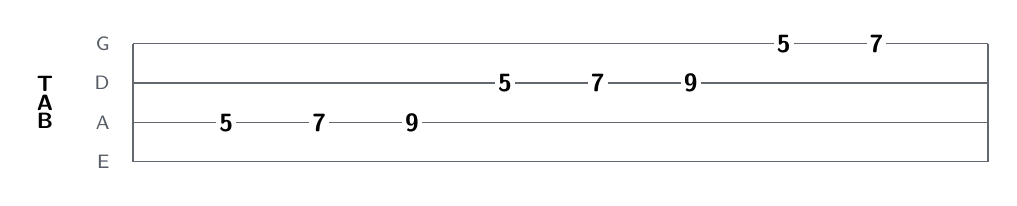
\begin{tikzpicture}[x=1.18cm,y=0.50cm]
\node[font=\sffamily\bfseries\footnotesize,align=center] at (-0.95,1.50) {T\\[-1mm]A\\[-1mm]B};
\foreach \y/\s in {3/G,2/D,1/A,0/E} {
  \draw[Ink!70,line width=0.55pt] (0,\y) -- (9.2,\y);
  \node[anchor=east,font=\sffamily\scriptsize,text=Ink!75] at (-0.15,\y) {\s};
}
\draw[Ink!70,line width=0.7pt] (0,0) -- (0,3);
\draw[Ink!70,line width=0.7pt] (9.2,0) -- (9.2,3);
\TabNum{1}{1}{5}
\TabNum{2}{1}{7}
\TabNum{3}{1}{9}
\TabNum{4}{2}{5}
\TabNum{5}{2}{7}
\TabNum{6}{2}{9}
\TabNum{7}{3}{5}
\TabNum{8}{3}{7}
\end{tikzpicture}
\endgroup
\end{center}

\begin{tabularx}{\textwidth}{>{\bfseries\sffamily}p{3.0cm}Y}
Signature sound & $\flat7$ over a major third \\
Harmonic fit & Dominant-7 chords, blues, funk, rock and salsa harmony \\
Overall colour & Major with dominant tension \\
Comparison & Major scale with 7 lowered to $\flat7$. \\
\end{tabularx}
\clearpage
\section{Locrian}
\begin{tabularx}{\textwidth}{>{\bfseries\sffamily}p{2.8cm}Y}
Formula & 1 $\flat2$ $\flat3$ 4 $\flat5$ $\flat6$ $\flat7$ \\
Step pattern & H -- W -- W -- H -- W -- W -- W \\
D example & D--E$\flat$--F--G--A$\flat$--B$\flat$--C--D \\
\end{tabularx}
\begin{center}
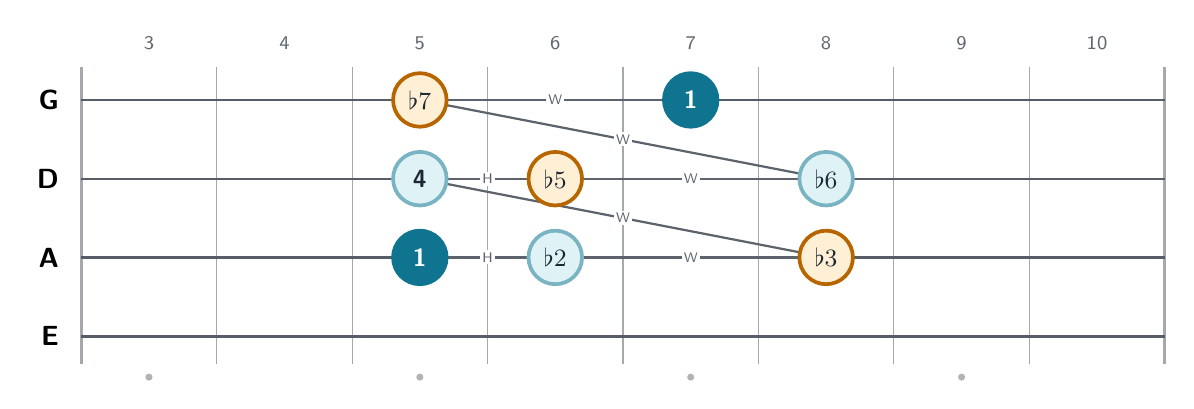
\begin{tikzpicture}[x=1cm,y=1cm,>=stealth]
\node[font=\sffamily\scriptsize,text=Ink!70] at (0.860,4.22) {3};
\node[font=\sffamily\scriptsize,text=Ink!70] at (2.580,4.22) {4};
\node[font=\sffamily\scriptsize,text=Ink!70] at (4.300,4.22) {5};
\node[font=\sffamily\scriptsize,text=Ink!70] at (6.020,4.22) {6};
\node[font=\sffamily\scriptsize,text=Ink!70] at (7.740,4.22) {7};
\node[font=\sffamily\scriptsize,text=Ink!70] at (9.460,4.22) {8};
\node[font=\sffamily\scriptsize,text=Ink!70] at (11.180,4.22) {9};
\node[font=\sffamily\scriptsize,text=Ink!70] at (12.900,4.22) {10};
\draw[Ink!40,line width=1.0pt] (0.000,0.15) -- (0.000,3.92);
\draw[Ink!40,line width=0.45pt] (1.720,0.15) -- (1.720,3.92);
\draw[Ink!40,line width=0.45pt] (3.440,0.15) -- (3.440,3.92);
\draw[Ink!40,line width=0.45pt] (5.160,0.15) -- (5.160,3.92);
\draw[Ink!40,line width=0.45pt] (6.880,0.15) -- (6.880,3.92);
\draw[Ink!40,line width=0.45pt] (8.600,0.15) -- (8.600,3.92);
\draw[Ink!40,line width=0.45pt] (10.320,0.15) -- (10.320,3.92);
\draw[Ink!40,line width=0.45pt] (12.040,0.15) -- (12.040,3.92);
\draw[Ink!40,line width=1.0pt] (13.760,0.15) -- (13.760,3.92);
\node[anchor=east,font=\sffamily\bfseries] at (-0.16,3.50) {G};
\draw[Ink!75,line width=0.45pt] (0,3.50) -- (13.760,3.50);
\node[anchor=east,font=\sffamily\bfseries] at (-0.16,2.50) {D};
\draw[Ink!75,line width=0.6pt] (0,2.50) -- (13.760,2.50);
\node[anchor=east,font=\sffamily\bfseries] at (-0.16,1.50) {A};
\draw[Ink!75,line width=0.8pt] (0,1.50) -- (13.760,1.50);
\node[anchor=east,font=\sffamily\bfseries] at (-0.16,0.50) {E};
\draw[Ink!75,line width=1.0pt] (0,0.50) -- (13.760,0.50);
\fill[Ink!35] (0.860,-0.02) circle (0.045);
\fill[Ink!35] (4.300,-0.02) circle (0.045);
\fill[Ink!35] (7.740,-0.02) circle (0.045);
\fill[Ink!35] (11.180,-0.02) circle (0.045);
\draw[->,Ink!72,line width=0.8pt] (4.300,1.500) -- node[midway,fill=white,inner sep=0.8pt,font=\sffamily\tiny] {H} (6.020,1.500);
\draw[->,Ink!72,line width=0.8pt] (6.020,1.500) -- node[midway,fill=white,inner sep=0.8pt,font=\sffamily\tiny] {W} (9.460,1.500);
\draw[->,Ink!72,line width=0.8pt] (9.460,1.500) -- node[midway,fill=white,inner sep=0.8pt,font=\sffamily\tiny] {W} (4.300,2.500);
\draw[->,Ink!72,line width=0.8pt] (4.300,2.500) -- node[midway,fill=white,inner sep=0.8pt,font=\sffamily\tiny] {H} (6.020,2.500);
\draw[->,Ink!72,line width=0.8pt] (6.020,2.500) -- node[midway,fill=white,inner sep=0.8pt,font=\sffamily\tiny] {W} (9.460,2.500);
\draw[->,Ink!72,line width=0.8pt] (9.460,2.500) -- node[midway,fill=white,inner sep=0.8pt,font=\sffamily\tiny] {W} (4.300,3.500);
\draw[->,Ink!72,line width=0.8pt] (4.300,3.500) -- node[midway,fill=white,inner sep=0.8pt,font=\sffamily\tiny] {W} (7.740,3.500);
\node[circle,minimum size=0.68cm,inner sep=0pt,fill=ChordLight,draw=Chord,line width=1.35pt,font=\sffamily\bfseries\small,text=Ink] at (4.300,3.500) {$\flat7$};
\node[circle,minimum size=0.68cm,inner sep=0pt,fill=Accent,draw=Accent,line width=1.35pt,font=\sffamily\bfseries\small,text=white] at (7.740,3.500) {1};
\node[circle,minimum size=0.68cm,inner sep=0pt,fill=AccentLight,draw=Accent!55,line width=1.35pt,font=\sffamily\bfseries\small,text=Ink] at (4.300,2.500) {4};
\node[circle,minimum size=0.68cm,inner sep=0pt,fill=ChordLight,draw=Chord,line width=1.35pt,font=\sffamily\bfseries\small,text=Ink] at (6.020,2.500) {$\flat5$};
\node[circle,minimum size=0.68cm,inner sep=0pt,fill=AccentLight,draw=Accent!55,line width=1.35pt,font=\sffamily\bfseries\small,text=Ink] at (9.460,2.500) {$\flat6$};
\node[circle,minimum size=0.68cm,inner sep=0pt,fill=Accent,draw=Accent,line width=1.35pt,font=\sffamily\bfseries\small,text=white] at (4.300,1.500) {1};
\node[circle,minimum size=0.68cm,inner sep=0pt,fill=AccentLight,draw=Accent!55,line width=1.35pt,font=\sffamily\bfseries\small,text=Ink] at (6.020,1.500) {$\flat2$};
\node[circle,minimum size=0.68cm,inner sep=0pt,fill=ChordLight,draw=Chord,line width=1.35pt,font=\sffamily\bfseries\small,text=Ink] at (9.460,1.500) {$\flat3$};
\end{tikzpicture}
\end{center}
\vspace{1mm}
\begin{center}
\begingroup
\setlength{\parindent}{0pt}
\begin{minipage}{0.82\textwidth}
{\sffamily\bfseries\small Standard notation}\par\vspace{-1mm}
\begin{music}
\instrumentnumber{1}
\setstaffs1{1}
\setclef1{\bass}
\nobarnumbers
\nostartrule
\startextract
\NOtes\qu K\qu{_L}\qu M\qu N\qu{_a}\qu{_b}\qu c\qu d\en
\zendextract
\end{music}
\end{minipage}
\vspace{-1mm}

{\sffamily\bfseries\small Bass TAB}\par\vspace{1mm}
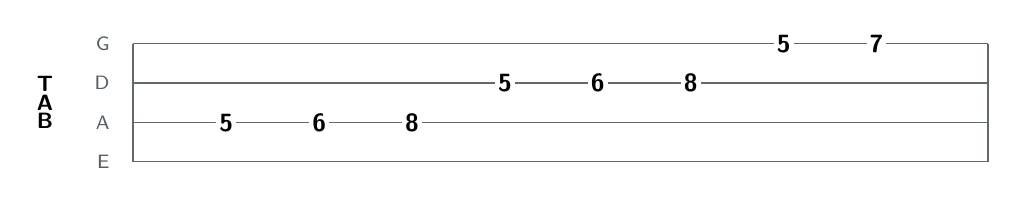
\begin{tikzpicture}[x=1.18cm,y=0.50cm]
\node[font=\sffamily\bfseries\footnotesize,align=center] at (-0.95,1.50) {T\\[-1mm]A\\[-1mm]B};
\foreach \y/\s in {3/G,2/D,1/A,0/E} {
  \draw[Ink!70,line width=0.55pt] (0,\y) -- (9.2,\y);
  \node[anchor=east,font=\sffamily\scriptsize,text=Ink!75] at (-0.15,\y) {\s};
}
\draw[Ink!70,line width=0.7pt] (0,0) -- (0,3);
\draw[Ink!70,line width=0.7pt] (9.2,0) -- (9.2,3);
\TabNum{1}{1}{5}
\TabNum{2}{1}{6}
\TabNum{3}{1}{8}
\TabNum{4}{2}{5}
\TabNum{5}{2}{6}
\TabNum{6}{2}{8}
\TabNum{7}{3}{5}
\TabNum{8}{3}{7}
\end{tikzpicture}
\endgroup
\end{center}

\begin{tabularx}{\textwidth}{>{\bfseries\sffamily}p{3.0cm}Y}
Signature sound & $\flat2$ and $\flat5$ \\
Harmonic fit & Half-diminished / minor-7-flat-5 chords \\
Overall colour & Unstable because the perfect fifth is absent \\
Comparison & Natural minor with 2 and 5 lowered. \\
\end{tabularx}
\clearpage
\section{Harmonic minor}
\begin{tabularx}{\textwidth}{>{\bfseries\sffamily}p{2.8cm}Y}
Formula & 1 2 $\flat3$ 4 5 $\flat6$ 7 \\
Step pattern & W -- H -- W -- W -- H -- A2 -- H \\
D example & D--E--F--G--A--B$\flat$--C\#--D \\
\end{tabularx}
\begin{center}
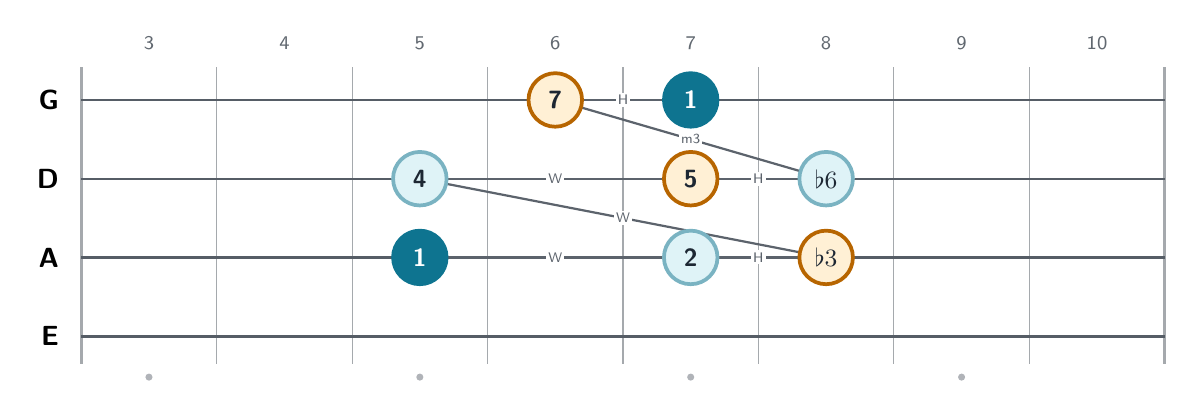
\begin{tikzpicture}[x=1cm,y=1cm,>=stealth]
\node[font=\sffamily\scriptsize,text=Ink!70] at (0.860,4.22) {3};
\node[font=\sffamily\scriptsize,text=Ink!70] at (2.580,4.22) {4};
\node[font=\sffamily\scriptsize,text=Ink!70] at (4.300,4.22) {5};
\node[font=\sffamily\scriptsize,text=Ink!70] at (6.020,4.22) {6};
\node[font=\sffamily\scriptsize,text=Ink!70] at (7.740,4.22) {7};
\node[font=\sffamily\scriptsize,text=Ink!70] at (9.460,4.22) {8};
\node[font=\sffamily\scriptsize,text=Ink!70] at (11.180,4.22) {9};
\node[font=\sffamily\scriptsize,text=Ink!70] at (12.900,4.22) {10};
\draw[Ink!40,line width=1.0pt] (0.000,0.15) -- (0.000,3.92);
\draw[Ink!40,line width=0.45pt] (1.720,0.15) -- (1.720,3.92);
\draw[Ink!40,line width=0.45pt] (3.440,0.15) -- (3.440,3.92);
\draw[Ink!40,line width=0.45pt] (5.160,0.15) -- (5.160,3.92);
\draw[Ink!40,line width=0.45pt] (6.880,0.15) -- (6.880,3.92);
\draw[Ink!40,line width=0.45pt] (8.600,0.15) -- (8.600,3.92);
\draw[Ink!40,line width=0.45pt] (10.320,0.15) -- (10.320,3.92);
\draw[Ink!40,line width=0.45pt] (12.040,0.15) -- (12.040,3.92);
\draw[Ink!40,line width=1.0pt] (13.760,0.15) -- (13.760,3.92);
\node[anchor=east,font=\sffamily\bfseries] at (-0.16,3.50) {G};
\draw[Ink!75,line width=0.45pt] (0,3.50) -- (13.760,3.50);
\node[anchor=east,font=\sffamily\bfseries] at (-0.16,2.50) {D};
\draw[Ink!75,line width=0.6pt] (0,2.50) -- (13.760,2.50);
\node[anchor=east,font=\sffamily\bfseries] at (-0.16,1.50) {A};
\draw[Ink!75,line width=0.8pt] (0,1.50) -- (13.760,1.50);
\node[anchor=east,font=\sffamily\bfseries] at (-0.16,0.50) {E};
\draw[Ink!75,line width=1.0pt] (0,0.50) -- (13.760,0.50);
\fill[Ink!35] (0.860,-0.02) circle (0.045);
\fill[Ink!35] (4.300,-0.02) circle (0.045);
\fill[Ink!35] (7.740,-0.02) circle (0.045);
\fill[Ink!35] (11.180,-0.02) circle (0.045);
\draw[->,Ink!72,line width=0.8pt] (4.300,1.500) -- node[midway,fill=white,inner sep=0.8pt,font=\sffamily\tiny] {W} (7.740,1.500);
\draw[->,Ink!72,line width=0.8pt] (7.740,1.500) -- node[midway,fill=white,inner sep=0.8pt,font=\sffamily\tiny] {H} (9.460,1.500);
\draw[->,Ink!72,line width=0.8pt] (9.460,1.500) -- node[midway,fill=white,inner sep=0.8pt,font=\sffamily\tiny] {W} (4.300,2.500);
\draw[->,Ink!72,line width=0.8pt] (4.300,2.500) -- node[midway,fill=white,inner sep=0.8pt,font=\sffamily\tiny] {W} (7.740,2.500);
\draw[->,Ink!72,line width=0.8pt] (7.740,2.500) -- node[midway,fill=white,inner sep=0.8pt,font=\sffamily\tiny] {H} (9.460,2.500);
\draw[->,Ink!72,line width=0.8pt] (9.460,2.500) -- node[midway,fill=white,inner sep=0.8pt,font=\sffamily\tiny] {m3} (6.020,3.500);
\draw[->,Ink!72,line width=0.8pt] (6.020,3.500) -- node[midway,fill=white,inner sep=0.8pt,font=\sffamily\tiny] {H} (7.740,3.500);
\node[circle,minimum size=0.68cm,inner sep=0pt,fill=ChordLight,draw=Chord,line width=1.35pt,font=\sffamily\bfseries\small,text=Ink] at (6.020,3.500) {7};
\node[circle,minimum size=0.68cm,inner sep=0pt,fill=Accent,draw=Accent,line width=1.35pt,font=\sffamily\bfseries\small,text=white] at (7.740,3.500) {1};
\node[circle,minimum size=0.68cm,inner sep=0pt,fill=AccentLight,draw=Accent!55,line width=1.35pt,font=\sffamily\bfseries\small,text=Ink] at (4.300,2.500) {4};
\node[circle,minimum size=0.68cm,inner sep=0pt,fill=ChordLight,draw=Chord,line width=1.35pt,font=\sffamily\bfseries\small,text=Ink] at (7.740,2.500) {5};
\node[circle,minimum size=0.68cm,inner sep=0pt,fill=AccentLight,draw=Accent!55,line width=1.35pt,font=\sffamily\bfseries\small,text=Ink] at (9.460,2.500) {$\flat6$};
\node[circle,minimum size=0.68cm,inner sep=0pt,fill=Accent,draw=Accent,line width=1.35pt,font=\sffamily\bfseries\small,text=white] at (4.300,1.500) {1};
\node[circle,minimum size=0.68cm,inner sep=0pt,fill=AccentLight,draw=Accent!55,line width=1.35pt,font=\sffamily\bfseries\small,text=Ink] at (7.740,1.500) {2};
\node[circle,minimum size=0.68cm,inner sep=0pt,fill=ChordLight,draw=Chord,line width=1.35pt,font=\sffamily\bfseries\small,text=Ink] at (9.460,1.500) {$\flat3$};
\end{tikzpicture}
\end{center}
\vspace{1mm}
\begin{center}
\begingroup
\setlength{\parindent}{0pt}
\begin{minipage}{0.82\textwidth}
{\sffamily\bfseries\small Standard notation}\par\vspace{-1mm}
\begin{music}
\instrumentnumber{1}
\setstaffs1{1}
\setclef1{\bass}
\nobarnumbers
\nostartrule
\startextract
\NOtes\qu K\qu L\qu M\qu N\qu a\qu{_b}\qu{^c}\qu d\en
\zendextract
\end{music}
\end{minipage}
\vspace{-1mm}

{\sffamily\bfseries\small Bass TAB}\par\vspace{1mm}
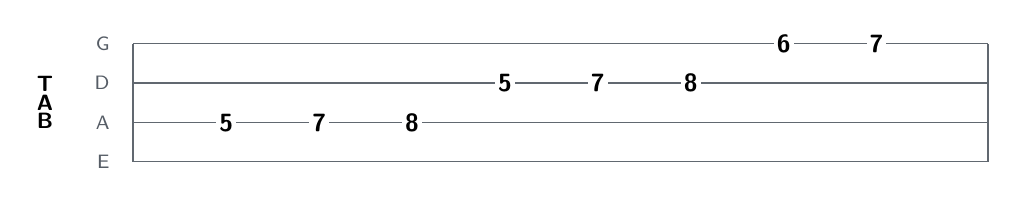
\begin{tikzpicture}[x=1.18cm,y=0.50cm]
\node[font=\sffamily\bfseries\footnotesize,align=center] at (-0.95,1.50) {T\\[-1mm]A\\[-1mm]B};
\foreach \y/\s in {3/G,2/D,1/A,0/E} {
  \draw[Ink!70,line width=0.55pt] (0,\y) -- (9.2,\y);
  \node[anchor=east,font=\sffamily\scriptsize,text=Ink!75] at (-0.15,\y) {\s};
}
\draw[Ink!70,line width=0.7pt] (0,0) -- (0,3);
\draw[Ink!70,line width=0.7pt] (9.2,0) -- (9.2,3);
\TabNum{1}{1}{5}
\TabNum{2}{1}{7}
\TabNum{3}{1}{8}
\TabNum{4}{2}{5}
\TabNum{5}{2}{7}
\TabNum{6}{2}{8}
\TabNum{7}{3}{6}
\TabNum{8}{3}{7}
\end{tikzpicture}
\endgroup
\end{center}

\begin{tabularx}{\textwidth}{>{\bfseries\sffamily}p{3.0cm}Y}
Signature sound & Raised 7 and the augmented second from $\flat6$ to 7 \\
Harmonic fit & Minor-key cadences; dominant V7 resolving to minor i \\
Overall colour & Minor with strong leading-tone pull \\
Comparison & Natural minor with $\flat7$ raised to 7. \\
\end{tabularx}
\clearpage
\section{Melodic minor}
\begin{tabularx}{\textwidth}{>{\bfseries\sffamily}p{2.8cm}Y}
Formula & 1 2 $\flat3$ 4 5 6 7 \\
Step pattern & W -- H -- W -- W -- W -- W -- H \\
D example & D--E--F--G--A--B--C\#--D \\
\end{tabularx}
\begin{center}
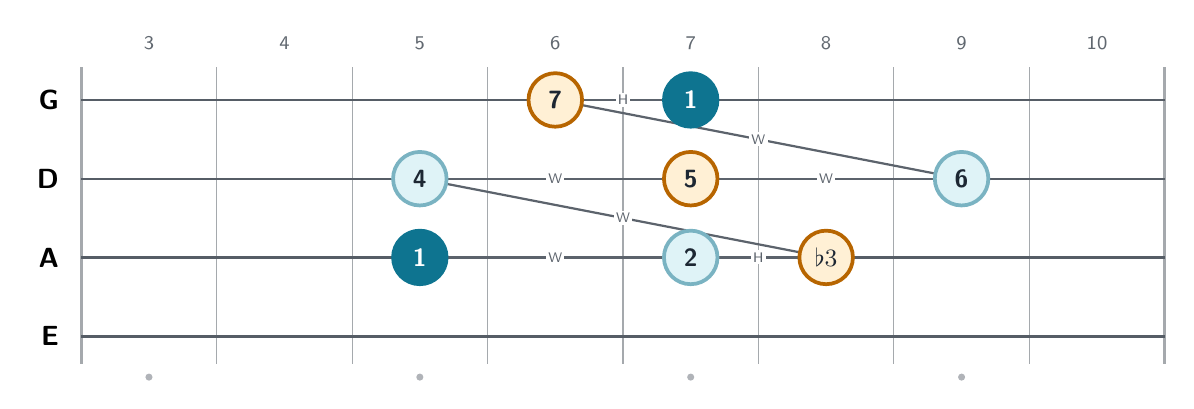
\begin{tikzpicture}[x=1cm,y=1cm,>=stealth]
\node[font=\sffamily\scriptsize,text=Ink!70] at (0.860,4.22) {3};
\node[font=\sffamily\scriptsize,text=Ink!70] at (2.580,4.22) {4};
\node[font=\sffamily\scriptsize,text=Ink!70] at (4.300,4.22) {5};
\node[font=\sffamily\scriptsize,text=Ink!70] at (6.020,4.22) {6};
\node[font=\sffamily\scriptsize,text=Ink!70] at (7.740,4.22) {7};
\node[font=\sffamily\scriptsize,text=Ink!70] at (9.460,4.22) {8};
\node[font=\sffamily\scriptsize,text=Ink!70] at (11.180,4.22) {9};
\node[font=\sffamily\scriptsize,text=Ink!70] at (12.900,4.22) {10};
\draw[Ink!40,line width=1.0pt] (0.000,0.15) -- (0.000,3.92);
\draw[Ink!40,line width=0.45pt] (1.720,0.15) -- (1.720,3.92);
\draw[Ink!40,line width=0.45pt] (3.440,0.15) -- (3.440,3.92);
\draw[Ink!40,line width=0.45pt] (5.160,0.15) -- (5.160,3.92);
\draw[Ink!40,line width=0.45pt] (6.880,0.15) -- (6.880,3.92);
\draw[Ink!40,line width=0.45pt] (8.600,0.15) -- (8.600,3.92);
\draw[Ink!40,line width=0.45pt] (10.320,0.15) -- (10.320,3.92);
\draw[Ink!40,line width=0.45pt] (12.040,0.15) -- (12.040,3.92);
\draw[Ink!40,line width=1.0pt] (13.760,0.15) -- (13.760,3.92);
\node[anchor=east,font=\sffamily\bfseries] at (-0.16,3.50) {G};
\draw[Ink!75,line width=0.45pt] (0,3.50) -- (13.760,3.50);
\node[anchor=east,font=\sffamily\bfseries] at (-0.16,2.50) {D};
\draw[Ink!75,line width=0.6pt] (0,2.50) -- (13.760,2.50);
\node[anchor=east,font=\sffamily\bfseries] at (-0.16,1.50) {A};
\draw[Ink!75,line width=0.8pt] (0,1.50) -- (13.760,1.50);
\node[anchor=east,font=\sffamily\bfseries] at (-0.16,0.50) {E};
\draw[Ink!75,line width=1.0pt] (0,0.50) -- (13.760,0.50);
\fill[Ink!35] (0.860,-0.02) circle (0.045);
\fill[Ink!35] (4.300,-0.02) circle (0.045);
\fill[Ink!35] (7.740,-0.02) circle (0.045);
\fill[Ink!35] (11.180,-0.02) circle (0.045);
\draw[->,Ink!72,line width=0.8pt] (4.300,1.500) -- node[midway,fill=white,inner sep=0.8pt,font=\sffamily\tiny] {W} (7.740,1.500);
\draw[->,Ink!72,line width=0.8pt] (7.740,1.500) -- node[midway,fill=white,inner sep=0.8pt,font=\sffamily\tiny] {H} (9.460,1.500);
\draw[->,Ink!72,line width=0.8pt] (9.460,1.500) -- node[midway,fill=white,inner sep=0.8pt,font=\sffamily\tiny] {W} (4.300,2.500);
\draw[->,Ink!72,line width=0.8pt] (4.300,2.500) -- node[midway,fill=white,inner sep=0.8pt,font=\sffamily\tiny] {W} (7.740,2.500);
\draw[->,Ink!72,line width=0.8pt] (7.740,2.500) -- node[midway,fill=white,inner sep=0.8pt,font=\sffamily\tiny] {W} (11.180,2.500);
\draw[->,Ink!72,line width=0.8pt] (11.180,2.500) -- node[midway,fill=white,inner sep=0.8pt,font=\sffamily\tiny] {W} (6.020,3.500);
\draw[->,Ink!72,line width=0.8pt] (6.020,3.500) -- node[midway,fill=white,inner sep=0.8pt,font=\sffamily\tiny] {H} (7.740,3.500);
\node[circle,minimum size=0.68cm,inner sep=0pt,fill=ChordLight,draw=Chord,line width=1.35pt,font=\sffamily\bfseries\small,text=Ink] at (6.020,3.500) {7};
\node[circle,minimum size=0.68cm,inner sep=0pt,fill=Accent,draw=Accent,line width=1.35pt,font=\sffamily\bfseries\small,text=white] at (7.740,3.500) {1};
\node[circle,minimum size=0.68cm,inner sep=0pt,fill=AccentLight,draw=Accent!55,line width=1.35pt,font=\sffamily\bfseries\small,text=Ink] at (4.300,2.500) {4};
\node[circle,minimum size=0.68cm,inner sep=0pt,fill=ChordLight,draw=Chord,line width=1.35pt,font=\sffamily\bfseries\small,text=Ink] at (7.740,2.500) {5};
\node[circle,minimum size=0.68cm,inner sep=0pt,fill=AccentLight,draw=Accent!55,line width=1.35pt,font=\sffamily\bfseries\small,text=Ink] at (11.180,2.500) {6};
\node[circle,minimum size=0.68cm,inner sep=0pt,fill=Accent,draw=Accent,line width=1.35pt,font=\sffamily\bfseries\small,text=white] at (4.300,1.500) {1};
\node[circle,minimum size=0.68cm,inner sep=0pt,fill=AccentLight,draw=Accent!55,line width=1.35pt,font=\sffamily\bfseries\small,text=Ink] at (7.740,1.500) {2};
\node[circle,minimum size=0.68cm,inner sep=0pt,fill=ChordLight,draw=Chord,line width=1.35pt,font=\sffamily\bfseries\small,text=Ink] at (9.460,1.500) {$\flat3$};
\end{tikzpicture}
\end{center}
\vspace{1mm}
\begin{center}
\begingroup
\setlength{\parindent}{0pt}
\begin{minipage}{0.82\textwidth}
{\sffamily\bfseries\small Standard notation}\par\vspace{-1mm}
\begin{music}
\instrumentnumber{1}
\setstaffs1{1}
\setclef1{\bass}
\nobarnumbers
\nostartrule
\startextract
\NOtes\qu K\qu L\qu M\qu N\qu a\qu b\qu{^c}\qu d\en
\zendextract
\end{music}
\end{minipage}
\vspace{-1mm}

{\sffamily\bfseries\small Bass TAB}\par\vspace{1mm}
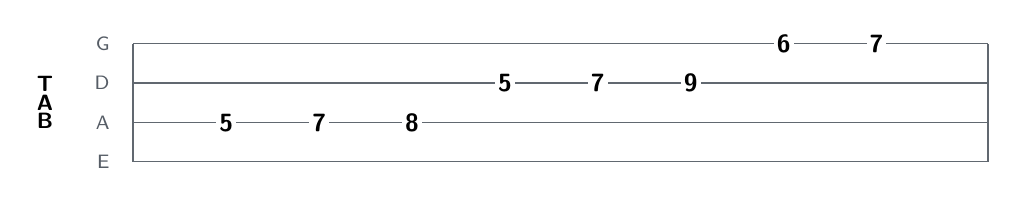
\begin{tikzpicture}[x=1.18cm,y=0.50cm]
\node[font=\sffamily\bfseries\footnotesize,align=center] at (-0.95,1.50) {T\\[-1mm]A\\[-1mm]B};
\foreach \y/\s in {3/G,2/D,1/A,0/E} {
  \draw[Ink!70,line width=0.55pt] (0,\y) -- (9.2,\y);
  \node[anchor=east,font=\sffamily\scriptsize,text=Ink!75] at (-0.15,\y) {\s};
}
\draw[Ink!70,line width=0.7pt] (0,0) -- (0,3);
\draw[Ink!70,line width=0.7pt] (9.2,0) -- (9.2,3);
\TabNum{1}{1}{5}
\TabNum{2}{1}{7}
\TabNum{3}{1}{8}
\TabNum{4}{2}{5}
\TabNum{5}{2}{7}
\TabNum{6}{2}{9}
\TabNum{7}{3}{6}
\TabNum{8}{3}{7}
\end{tikzpicture}
\endgroup
\end{center}

\begin{tabularx}{\textwidth}{>{\bfseries\sffamily}p{3.0cm}Y}
Signature sound & $\flat3$ with natural 6 and 7 \\
Harmonic fit & Minor-major-7 harmony and modern jazz sounds \\
Overall colour & Minor tonic with a smooth upper half \\
Comparison & Diagram uses the ascending/jazz form; classical descent often uses natural minor. \\
\end{tabularx}
\clearpage
\section{Major pentatonic}\label{scale:major-pent}
\begin{tabularx}{\textwidth}{>{\bfseries\sffamily}p{2.8cm}Y}
Formula & 1 2 3 5 6 \\
Step pattern & W -- W -- m3 -- W -- m3 \\
D example & D--E--F\#--A--B--D \\
\end{tabularx}
\begin{center}
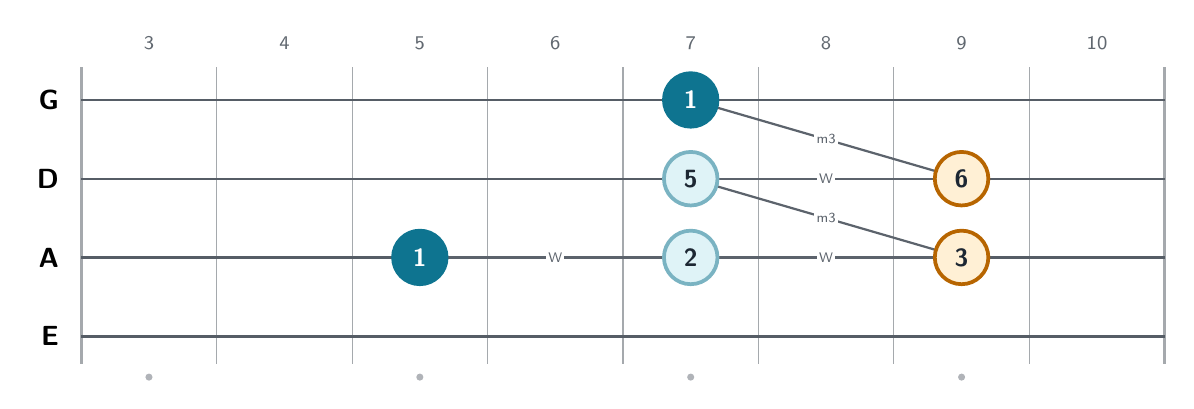
\begin{tikzpicture}[x=1cm,y=1cm,>=stealth]
\node[font=\sffamily\scriptsize,text=Ink!70] at (0.860,4.22) {3};
\node[font=\sffamily\scriptsize,text=Ink!70] at (2.580,4.22) {4};
\node[font=\sffamily\scriptsize,text=Ink!70] at (4.300,4.22) {5};
\node[font=\sffamily\scriptsize,text=Ink!70] at (6.020,4.22) {6};
\node[font=\sffamily\scriptsize,text=Ink!70] at (7.740,4.22) {7};
\node[font=\sffamily\scriptsize,text=Ink!70] at (9.460,4.22) {8};
\node[font=\sffamily\scriptsize,text=Ink!70] at (11.180,4.22) {9};
\node[font=\sffamily\scriptsize,text=Ink!70] at (12.900,4.22) {10};
\draw[Ink!40,line width=1.0pt] (0.000,0.15) -- (0.000,3.92);
\draw[Ink!40,line width=0.45pt] (1.720,0.15) -- (1.720,3.92);
\draw[Ink!40,line width=0.45pt] (3.440,0.15) -- (3.440,3.92);
\draw[Ink!40,line width=0.45pt] (5.160,0.15) -- (5.160,3.92);
\draw[Ink!40,line width=0.45pt] (6.880,0.15) -- (6.880,3.92);
\draw[Ink!40,line width=0.45pt] (8.600,0.15) -- (8.600,3.92);
\draw[Ink!40,line width=0.45pt] (10.320,0.15) -- (10.320,3.92);
\draw[Ink!40,line width=0.45pt] (12.040,0.15) -- (12.040,3.92);
\draw[Ink!40,line width=1.0pt] (13.760,0.15) -- (13.760,3.92);
\node[anchor=east,font=\sffamily\bfseries] at (-0.16,3.50) {G};
\draw[Ink!75,line width=0.45pt] (0,3.50) -- (13.760,3.50);
\node[anchor=east,font=\sffamily\bfseries] at (-0.16,2.50) {D};
\draw[Ink!75,line width=0.6pt] (0,2.50) -- (13.760,2.50);
\node[anchor=east,font=\sffamily\bfseries] at (-0.16,1.50) {A};
\draw[Ink!75,line width=0.8pt] (0,1.50) -- (13.760,1.50);
\node[anchor=east,font=\sffamily\bfseries] at (-0.16,0.50) {E};
\draw[Ink!75,line width=1.0pt] (0,0.50) -- (13.760,0.50);
\fill[Ink!35] (0.860,-0.02) circle (0.045);
\fill[Ink!35] (4.300,-0.02) circle (0.045);
\fill[Ink!35] (7.740,-0.02) circle (0.045);
\fill[Ink!35] (11.180,-0.02) circle (0.045);
\draw[->,Ink!72,line width=0.8pt] (4.300,1.500) -- node[midway,fill=white,inner sep=0.8pt,font=\sffamily\tiny] {W} (7.740,1.500);
\draw[->,Ink!72,line width=0.8pt] (7.740,1.500) -- node[midway,fill=white,inner sep=0.8pt,font=\sffamily\tiny] {W} (11.180,1.500);
\draw[->,Ink!72,line width=0.8pt] (11.180,1.500) -- node[midway,fill=white,inner sep=0.8pt,font=\sffamily\tiny] {m3} (7.740,2.500);
\draw[->,Ink!72,line width=0.8pt] (7.740,2.500) -- node[midway,fill=white,inner sep=0.8pt,font=\sffamily\tiny] {W} (11.180,2.500);
\draw[->,Ink!72,line width=0.8pt] (11.180,2.500) -- node[midway,fill=white,inner sep=0.8pt,font=\sffamily\tiny] {m3} (7.740,3.500);
\node[circle,minimum size=0.68cm,inner sep=0pt,fill=Accent,draw=Accent,line width=1.35pt,font=\sffamily\bfseries\small,text=white] at (7.740,3.500) {1};
\node[circle,minimum size=0.68cm,inner sep=0pt,fill=AccentLight,draw=Accent!55,line width=1.35pt,font=\sffamily\bfseries\small,text=Ink] at (7.740,2.500) {5};
\node[circle,minimum size=0.68cm,inner sep=0pt,fill=ChordLight,draw=Chord,line width=1.35pt,font=\sffamily\bfseries\small,text=Ink] at (11.180,2.500) {6};
\node[circle,minimum size=0.68cm,inner sep=0pt,fill=Accent,draw=Accent,line width=1.35pt,font=\sffamily\bfseries\small,text=white] at (4.300,1.500) {1};
\node[circle,minimum size=0.68cm,inner sep=0pt,fill=AccentLight,draw=Accent!55,line width=1.35pt,font=\sffamily\bfseries\small,text=Ink] at (7.740,1.500) {2};
\node[circle,minimum size=0.68cm,inner sep=0pt,fill=ChordLight,draw=Chord,line width=1.35pt,font=\sffamily\bfseries\small,text=Ink] at (11.180,1.500) {3};
\end{tikzpicture}
\end{center}
\vspace{1mm}
\begin{center}
\begingroup
\setlength{\parindent}{0pt}
\begin{minipage}{0.82\textwidth}
{\sffamily\bfseries\small Standard notation}\par\vspace{-1mm}
\begin{music}
\instrumentnumber{1}
\setstaffs1{1}
\setclef1{\bass}
\nobarnumbers
\nostartrule
\startextract
\NOtes\qu K\qu L\qu{^M}\qu a\qu b\qu d\en
\zendextract
\end{music}
\end{minipage}
\vspace{-1mm}

{\sffamily\bfseries\small Bass TAB}\par\vspace{1mm}
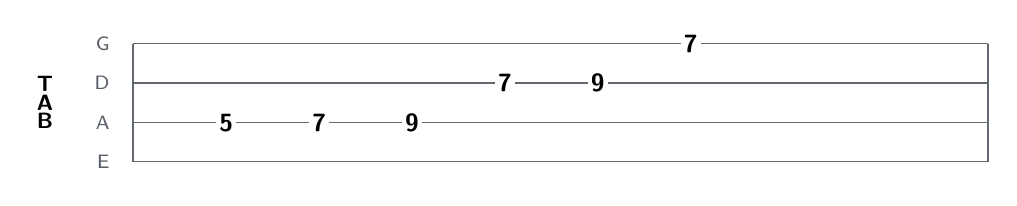
\begin{tikzpicture}[x=1.18cm,y=0.50cm]
\node[font=\sffamily\bfseries\footnotesize,align=center] at (-0.95,1.50) {T\\[-1mm]A\\[-1mm]B};
\foreach \y/\s in {3/G,2/D,1/A,0/E} {
  \draw[Ink!70,line width=0.55pt] (0,\y) -- (9.2,\y);
  \node[anchor=east,font=\sffamily\scriptsize,text=Ink!75] at (-0.15,\y) {\s};
}
\draw[Ink!70,line width=0.7pt] (0,0) -- (0,3);
\draw[Ink!70,line width=0.7pt] (9.2,0) -- (9.2,3);
\TabNum{1}{1}{5}
\TabNum{2}{1}{7}
\TabNum{3}{1}{9}
\TabNum{4}{2}{7}
\TabNum{5}{2}{9}
\TabNum{6}{3}{7}
\end{tikzpicture}
\endgroup
\end{center}

\begin{tabularx}{\textwidth}{>{\bfseries\sffamily}p{3.0cm}Y}
Signature sound & No 4 or 7 \\
Harmonic fit & Major chords, melodic fills, country, soul and pop \\
Overall colour & Open and consonant \\
Comparison & Major scale with 4 and 7 removed. \\
\end{tabularx}
\clearpage
\section{Minor pentatonic}\label{scale:minor-pent}
\begin{tabularx}{\textwidth}{>{\bfseries\sffamily}p{2.8cm}Y}
Formula & 1 $\flat3$ 4 5 $\flat7$ \\
Step pattern & m3 -- W -- W -- m3 -- W \\
D example & D--F--G--A--C--D \\
\end{tabularx}
\begin{center}
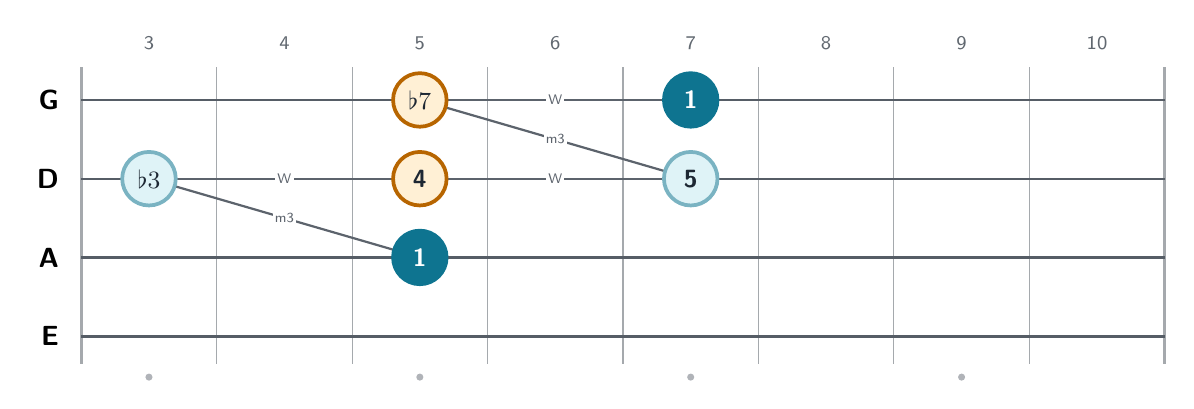
\begin{tikzpicture}[x=1cm,y=1cm,>=stealth]
\node[font=\sffamily\scriptsize,text=Ink!70] at (0.860,4.22) {3};
\node[font=\sffamily\scriptsize,text=Ink!70] at (2.580,4.22) {4};
\node[font=\sffamily\scriptsize,text=Ink!70] at (4.300,4.22) {5};
\node[font=\sffamily\scriptsize,text=Ink!70] at (6.020,4.22) {6};
\node[font=\sffamily\scriptsize,text=Ink!70] at (7.740,4.22) {7};
\node[font=\sffamily\scriptsize,text=Ink!70] at (9.460,4.22) {8};
\node[font=\sffamily\scriptsize,text=Ink!70] at (11.180,4.22) {9};
\node[font=\sffamily\scriptsize,text=Ink!70] at (12.900,4.22) {10};
\draw[Ink!40,line width=1.0pt] (0.000,0.15) -- (0.000,3.92);
\draw[Ink!40,line width=0.45pt] (1.720,0.15) -- (1.720,3.92);
\draw[Ink!40,line width=0.45pt] (3.440,0.15) -- (3.440,3.92);
\draw[Ink!40,line width=0.45pt] (5.160,0.15) -- (5.160,3.92);
\draw[Ink!40,line width=0.45pt] (6.880,0.15) -- (6.880,3.92);
\draw[Ink!40,line width=0.45pt] (8.600,0.15) -- (8.600,3.92);
\draw[Ink!40,line width=0.45pt] (10.320,0.15) -- (10.320,3.92);
\draw[Ink!40,line width=0.45pt] (12.040,0.15) -- (12.040,3.92);
\draw[Ink!40,line width=1.0pt] (13.760,0.15) -- (13.760,3.92);
\node[anchor=east,font=\sffamily\bfseries] at (-0.16,3.50) {G};
\draw[Ink!75,line width=0.45pt] (0,3.50) -- (13.760,3.50);
\node[anchor=east,font=\sffamily\bfseries] at (-0.16,2.50) {D};
\draw[Ink!75,line width=0.6pt] (0,2.50) -- (13.760,2.50);
\node[anchor=east,font=\sffamily\bfseries] at (-0.16,1.50) {A};
\draw[Ink!75,line width=0.8pt] (0,1.50) -- (13.760,1.50);
\node[anchor=east,font=\sffamily\bfseries] at (-0.16,0.50) {E};
\draw[Ink!75,line width=1.0pt] (0,0.50) -- (13.760,0.50);
\fill[Ink!35] (0.860,-0.02) circle (0.045);
\fill[Ink!35] (4.300,-0.02) circle (0.045);
\fill[Ink!35] (7.740,-0.02) circle (0.045);
\fill[Ink!35] (11.180,-0.02) circle (0.045);
\draw[->,Ink!72,line width=0.8pt] (4.300,1.500) -- node[midway,fill=white,inner sep=0.8pt,font=\sffamily\tiny] {m3} (0.860,2.500);
\draw[->,Ink!72,line width=0.8pt] (0.860,2.500) -- node[midway,fill=white,inner sep=0.8pt,font=\sffamily\tiny] {W} (4.300,2.500);
\draw[->,Ink!72,line width=0.8pt] (4.300,2.500) -- node[midway,fill=white,inner sep=0.8pt,font=\sffamily\tiny] {W} (7.740,2.500);
\draw[->,Ink!72,line width=0.8pt] (7.740,2.500) -- node[midway,fill=white,inner sep=0.8pt,font=\sffamily\tiny] {m3} (4.300,3.500);
\draw[->,Ink!72,line width=0.8pt] (4.300,3.500) -- node[midway,fill=white,inner sep=0.8pt,font=\sffamily\tiny] {W} (7.740,3.500);
\node[circle,minimum size=0.68cm,inner sep=0pt,fill=ChordLight,draw=Chord,line width=1.35pt,font=\sffamily\bfseries\small,text=Ink] at (4.300,3.500) {$\flat7$};
\node[circle,minimum size=0.68cm,inner sep=0pt,fill=Accent,draw=Accent,line width=1.35pt,font=\sffamily\bfseries\small,text=white] at (7.740,3.500) {1};
\node[circle,minimum size=0.68cm,inner sep=0pt,fill=AccentLight,draw=Accent!55,line width=1.35pt,font=\sffamily\bfseries\small,text=Ink] at (0.860,2.500) {$\flat3$};
\node[circle,minimum size=0.68cm,inner sep=0pt,fill=ChordLight,draw=Chord,line width=1.35pt,font=\sffamily\bfseries\small,text=Ink] at (4.300,2.500) {4};
\node[circle,minimum size=0.68cm,inner sep=0pt,fill=AccentLight,draw=Accent!55,line width=1.35pt,font=\sffamily\bfseries\small,text=Ink] at (7.740,2.500) {5};
\node[circle,minimum size=0.68cm,inner sep=0pt,fill=Accent,draw=Accent,line width=1.35pt,font=\sffamily\bfseries\small,text=white] at (4.300,1.500) {1};
\end{tikzpicture}
\end{center}
\vspace{1mm}
\begin{center}
\begingroup
\setlength{\parindent}{0pt}
\begin{minipage}{0.82\textwidth}
{\sffamily\bfseries\small Standard notation}\par\vspace{-1mm}
\begin{music}
\instrumentnumber{1}
\setstaffs1{1}
\setclef1{\bass}
\nobarnumbers
\nostartrule
\startextract
\NOtes\qu K\qu M\qu N\qu a\qu c\qu d\en
\zendextract
\end{music}
\end{minipage}
\vspace{-1mm}

{\sffamily\bfseries\small Bass TAB}\par\vspace{1mm}
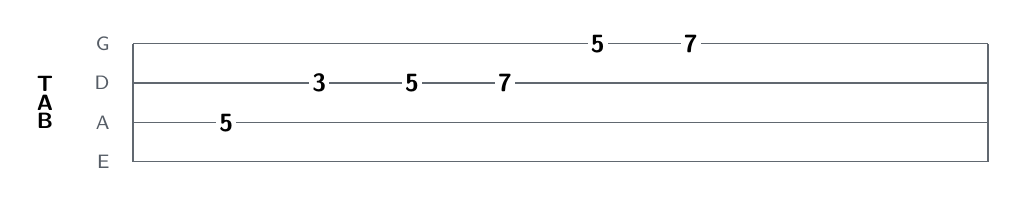
\begin{tikzpicture}[x=1.18cm,y=0.50cm]
\node[font=\sffamily\bfseries\footnotesize,align=center] at (-0.95,1.50) {T\\[-1mm]A\\[-1mm]B};
\foreach \y/\s in {3/G,2/D,1/A,0/E} {
  \draw[Ink!70,line width=0.55pt] (0,\y) -- (9.2,\y);
  \node[anchor=east,font=\sffamily\scriptsize,text=Ink!75] at (-0.15,\y) {\s};
}
\draw[Ink!70,line width=0.7pt] (0,0) -- (0,3);
\draw[Ink!70,line width=0.7pt] (9.2,0) -- (9.2,3);
\TabNum{1}{1}{5}
\TabNum{2}{2}{3}
\TabNum{3}{2}{5}
\TabNum{4}{2}{7}
\TabNum{5}{3}{5}
\TabNum{6}{3}{7}
\end{tikzpicture}
\endgroup
\end{center}

\begin{tabularx}{\textwidth}{>{\bfseries\sffamily}p{3.0cm}Y}
Signature sound & $\flat3$ and $\flat7$; no 2 or 6 \\
Harmonic fit & Minor grooves, blues, rock and funk \\
Overall colour & Strong, compact minor vocabulary \\
Comparison & Natural minor with 2 and $\flat6$ removed. \\
\end{tabularx}
\clearpage
\section{Blues scale}\label{scale:blues}
\begin{tabularx}{\textwidth}{>{\bfseries\sffamily}p{2.8cm}Y}
Formula & 1 $\flat3$ 4 $\flat5$ 5 $\flat7$ \\
Step pattern & m3 -- W -- H -- H -- m3 -- W \\
D example & D--F--G--A$\flat$--A--C--D \\
\end{tabularx}
\begin{center}
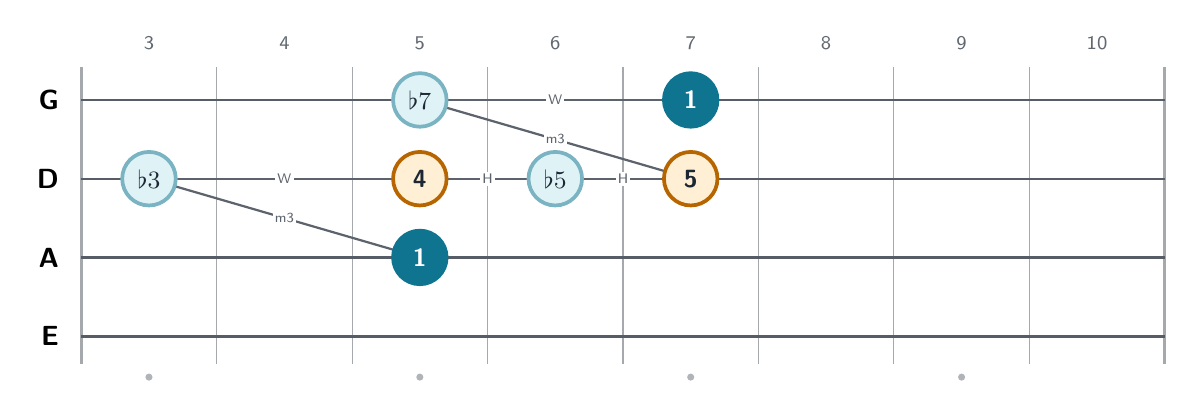
\begin{tikzpicture}[x=1cm,y=1cm,>=stealth]
\node[font=\sffamily\scriptsize,text=Ink!70] at (0.860,4.22) {3};
\node[font=\sffamily\scriptsize,text=Ink!70] at (2.580,4.22) {4};
\node[font=\sffamily\scriptsize,text=Ink!70] at (4.300,4.22) {5};
\node[font=\sffamily\scriptsize,text=Ink!70] at (6.020,4.22) {6};
\node[font=\sffamily\scriptsize,text=Ink!70] at (7.740,4.22) {7};
\node[font=\sffamily\scriptsize,text=Ink!70] at (9.460,4.22) {8};
\node[font=\sffamily\scriptsize,text=Ink!70] at (11.180,4.22) {9};
\node[font=\sffamily\scriptsize,text=Ink!70] at (12.900,4.22) {10};
\draw[Ink!40,line width=1.0pt] (0.000,0.15) -- (0.000,3.92);
\draw[Ink!40,line width=0.45pt] (1.720,0.15) -- (1.720,3.92);
\draw[Ink!40,line width=0.45pt] (3.440,0.15) -- (3.440,3.92);
\draw[Ink!40,line width=0.45pt] (5.160,0.15) -- (5.160,3.92);
\draw[Ink!40,line width=0.45pt] (6.880,0.15) -- (6.880,3.92);
\draw[Ink!40,line width=0.45pt] (8.600,0.15) -- (8.600,3.92);
\draw[Ink!40,line width=0.45pt] (10.320,0.15) -- (10.320,3.92);
\draw[Ink!40,line width=0.45pt] (12.040,0.15) -- (12.040,3.92);
\draw[Ink!40,line width=1.0pt] (13.760,0.15) -- (13.760,3.92);
\node[anchor=east,font=\sffamily\bfseries] at (-0.16,3.50) {G};
\draw[Ink!75,line width=0.45pt] (0,3.50) -- (13.760,3.50);
\node[anchor=east,font=\sffamily\bfseries] at (-0.16,2.50) {D};
\draw[Ink!75,line width=0.6pt] (0,2.50) -- (13.760,2.50);
\node[anchor=east,font=\sffamily\bfseries] at (-0.16,1.50) {A};
\draw[Ink!75,line width=0.8pt] (0,1.50) -- (13.760,1.50);
\node[anchor=east,font=\sffamily\bfseries] at (-0.16,0.50) {E};
\draw[Ink!75,line width=1.0pt] (0,0.50) -- (13.760,0.50);
\fill[Ink!35] (0.860,-0.02) circle (0.045);
\fill[Ink!35] (4.300,-0.02) circle (0.045);
\fill[Ink!35] (7.740,-0.02) circle (0.045);
\fill[Ink!35] (11.180,-0.02) circle (0.045);
\draw[->,Ink!72,line width=0.8pt] (4.300,1.500) -- node[midway,fill=white,inner sep=0.8pt,font=\sffamily\tiny] {m3} (0.860,2.500);
\draw[->,Ink!72,line width=0.8pt] (0.860,2.500) -- node[midway,fill=white,inner sep=0.8pt,font=\sffamily\tiny] {W} (4.300,2.500);
\draw[->,Ink!72,line width=0.8pt] (4.300,2.500) -- node[midway,fill=white,inner sep=0.8pt,font=\sffamily\tiny] {H} (6.020,2.500);
\draw[->,Ink!72,line width=0.8pt] (6.020,2.500) -- node[midway,fill=white,inner sep=0.8pt,font=\sffamily\tiny] {H} (7.740,2.500);
\draw[->,Ink!72,line width=0.8pt] (7.740,2.500) -- node[midway,fill=white,inner sep=0.8pt,font=\sffamily\tiny] {m3} (4.300,3.500);
\draw[->,Ink!72,line width=0.8pt] (4.300,3.500) -- node[midway,fill=white,inner sep=0.8pt,font=\sffamily\tiny] {W} (7.740,3.500);
\node[circle,minimum size=0.68cm,inner sep=0pt,fill=AccentLight,draw=Accent!55,line width=1.35pt,font=\sffamily\bfseries\small,text=Ink] at (4.300,3.500) {$\flat7$};
\node[circle,minimum size=0.68cm,inner sep=0pt,fill=Accent,draw=Accent,line width=1.35pt,font=\sffamily\bfseries\small,text=white] at (7.740,3.500) {1};
\node[circle,minimum size=0.68cm,inner sep=0pt,fill=AccentLight,draw=Accent!55,line width=1.35pt,font=\sffamily\bfseries\small,text=Ink] at (0.860,2.500) {$\flat3$};
\node[circle,minimum size=0.68cm,inner sep=0pt,fill=ChordLight,draw=Chord,line width=1.35pt,font=\sffamily\bfseries\small,text=Ink] at (4.300,2.500) {4};
\node[circle,minimum size=0.68cm,inner sep=0pt,fill=AccentLight,draw=Accent!55,line width=1.35pt,font=\sffamily\bfseries\small,text=Ink] at (6.020,2.500) {$\flat5$};
\node[circle,minimum size=0.68cm,inner sep=0pt,fill=ChordLight,draw=Chord,line width=1.35pt,font=\sffamily\bfseries\small,text=Ink] at (7.740,2.500) {5};
\node[circle,minimum size=0.68cm,inner sep=0pt,fill=Accent,draw=Accent,line width=1.35pt,font=\sffamily\bfseries\small,text=white] at (4.300,1.500) {1};
\end{tikzpicture}
\end{center}
\vspace{1mm}
\begin{center}
\begingroup
\setlength{\parindent}{0pt}
\begin{minipage}{0.82\textwidth}
{\sffamily\bfseries\small Standard notation}\par\vspace{-1mm}
\begin{music}
\instrumentnumber{1}
\setstaffs1{1}
\setclef1{\bass}
\nobarnumbers
\nostartrule
\startextract
\NOtes\qu K\qu M\qu N\qu{_a}\qu a\qu c\qu d\en
\zendextract
\end{music}
\end{minipage}
\vspace{-1mm}

{\sffamily\bfseries\small Bass TAB}\par\vspace{1mm}
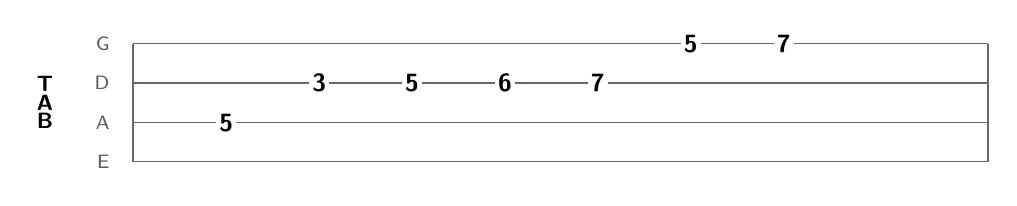
\begin{tikzpicture}[x=1.18cm,y=0.50cm]
\node[font=\sffamily\bfseries\footnotesize,align=center] at (-0.95,1.50) {T\\[-1mm]A\\[-1mm]B};
\foreach \y/\s in {3/G,2/D,1/A,0/E} {
  \draw[Ink!70,line width=0.55pt] (0,\y) -- (9.2,\y);
  \node[anchor=east,font=\sffamily\scriptsize,text=Ink!75] at (-0.15,\y) {\s};
}
\draw[Ink!70,line width=0.7pt] (0,0) -- (0,3);
\draw[Ink!70,line width=0.7pt] (9.2,0) -- (9.2,3);
\TabNum{1}{1}{5}
\TabNum{2}{2}{3}
\TabNum{3}{2}{5}
\TabNum{4}{2}{6}
\TabNum{5}{2}{7}
\TabNum{6}{3}{5}
\TabNum{7}{3}{7}
\end{tikzpicture}
\endgroup
\end{center}

\begin{tabularx}{\textwidth}{>{\bfseries\sffamily}p{3.0cm}Y}
Signature sound & $\flat5$ passing between 4 and 5 \\
Harmonic fit & Blues language and tension inside minor-pentatonic lines \\
Overall colour & Minor pentatonic with an added chromatic pull \\
Comparison & Minor pentatonic plus $\flat5$. \\
\end{tabularx}
\clearpage
\section{Chord-tone arpeggio atlas}
\begin{keybox}
Scales describe the available pitch collection; arpeggios show the chord itself. In bass lines, roots, thirds, fifths and sevenths usually carry more harmonic information than the remaining scale tones.
\end{keybox}
\subsection{Major triad}
\begin{tabularx}{\textwidth}{>{\bfseries\sffamily}p{2.5cm}Y}
Formula & 1 3 5 \quad Example: D--F\#--A--D \quad Use: Major chord skeleton \\
\end{tabularx}
\begin{center}
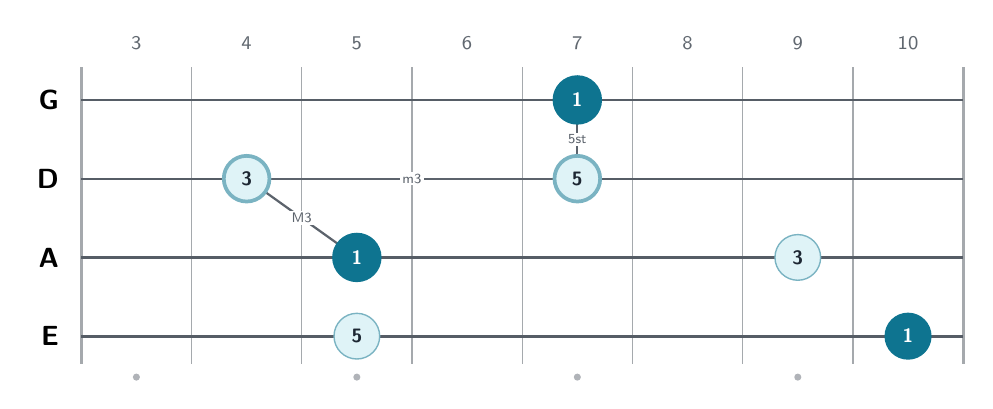
\begin{tikzpicture}[x=1cm,y=1cm,>=stealth]
\node[font=\sffamily\scriptsize,text=Ink!70] at (0.700,4.22) {3};
\node[font=\sffamily\scriptsize,text=Ink!70] at (2.100,4.22) {4};
\node[font=\sffamily\scriptsize,text=Ink!70] at (3.500,4.22) {5};
\node[font=\sffamily\scriptsize,text=Ink!70] at (4.900,4.22) {6};
\node[font=\sffamily\scriptsize,text=Ink!70] at (6.300,4.22) {7};
\node[font=\sffamily\scriptsize,text=Ink!70] at (7.700,4.22) {8};
\node[font=\sffamily\scriptsize,text=Ink!70] at (9.100,4.22) {9};
\node[font=\sffamily\scriptsize,text=Ink!70] at (10.500,4.22) {10};
\draw[Ink!40,line width=1.0pt] (0.000,0.15) -- (0.000,3.92);
\draw[Ink!40,line width=0.45pt] (1.400,0.15) -- (1.400,3.92);
\draw[Ink!40,line width=0.45pt] (2.800,0.15) -- (2.800,3.92);
\draw[Ink!40,line width=0.45pt] (4.200,0.15) -- (4.200,3.92);
\draw[Ink!40,line width=0.45pt] (5.600,0.15) -- (5.600,3.92);
\draw[Ink!40,line width=0.45pt] (7.000,0.15) -- (7.000,3.92);
\draw[Ink!40,line width=0.45pt] (8.400,0.15) -- (8.400,3.92);
\draw[Ink!40,line width=0.45pt] (9.800,0.15) -- (9.800,3.92);
\draw[Ink!40,line width=1.0pt] (11.200,0.15) -- (11.200,3.92);
\node[anchor=east,font=\sffamily\bfseries] at (-0.16,3.50) {G};
\draw[Ink!75,line width=0.45pt] (0,3.50) -- (11.200,3.50);
\node[anchor=east,font=\sffamily\bfseries] at (-0.16,2.50) {D};
\draw[Ink!75,line width=0.6pt] (0,2.50) -- (11.200,2.50);
\node[anchor=east,font=\sffamily\bfseries] at (-0.16,1.50) {A};
\draw[Ink!75,line width=0.8pt] (0,1.50) -- (11.200,1.50);
\node[anchor=east,font=\sffamily\bfseries] at (-0.16,0.50) {E};
\draw[Ink!75,line width=1.0pt] (0,0.50) -- (11.200,0.50);
\fill[Ink!35] (0.700,-0.02) circle (0.045);
\fill[Ink!35] (3.500,-0.02) circle (0.045);
\fill[Ink!35] (6.300,-0.02) circle (0.045);
\fill[Ink!35] (9.100,-0.02) circle (0.045);
\draw[->,Ink!72,line width=0.8pt] (3.500,1.500) -- node[midway,fill=white,inner sep=0.8pt,font=\sffamily\tiny] {M3} (2.100,2.500);
\draw[->,Ink!72,line width=0.8pt] (2.100,2.500) -- node[midway,fill=white,inner sep=0.8pt,font=\sffamily\tiny] {m3} (6.300,2.500);
\draw[->,Ink!72,line width=0.8pt] (6.300,2.500) -- node[midway,fill=white,inner sep=0.8pt,font=\sffamily\tiny] {5st} (6.300,3.500);
\node[circle,minimum size=0.58cm,inner sep=0pt,fill=Accent,draw=Accent,line width=1.35pt,font=\sffamily\bfseries\scriptsize,text=white] at (6.300,3.500) {1};
\node[circle,minimum size=0.58cm,inner sep=0pt,fill=AccentLight,draw=Accent!55,line width=1.35pt,font=\sffamily\bfseries\scriptsize,text=Ink] at (2.100,2.500) {3};
\node[circle,minimum size=0.58cm,inner sep=0pt,fill=AccentLight,draw=Accent!55,line width=1.35pt,font=\sffamily\bfseries\scriptsize,text=Ink] at (6.300,2.500) {5};
\node[circle,minimum size=0.58cm,inner sep=0pt,fill=Accent,draw=Accent,line width=1.35pt,font=\sffamily\bfseries\scriptsize,text=white] at (3.500,1.500) {1};
\node[circle,minimum size=0.58cm,inner sep=0pt,fill=AccentLight,draw=Accent!55,line width=0.5pt,font=\sffamily\bfseries\scriptsize,text=Ink] at (9.100,1.500) {3};
\node[circle,minimum size=0.58cm,inner sep=0pt,fill=AccentLight,draw=Accent!55,line width=0.5pt,font=\sffamily\bfseries\scriptsize,text=Ink] at (3.500,0.500) {5};
\node[circle,minimum size=0.58cm,inner sep=0pt,fill=Accent,draw=Accent,line width=0.5pt,font=\sffamily\bfseries\scriptsize,text=white] at (10.500,0.500) {1};
\end{tikzpicture}
\end{center}
\subsection{Minor triad}
\begin{tabularx}{\textwidth}{>{\bfseries\sffamily}p{2.5cm}Y}
Formula & 1 $\flat3$ 5 \quad Example: D--F--A--D \quad Use: Minor chord skeleton \\
\end{tabularx}
\begin{center}
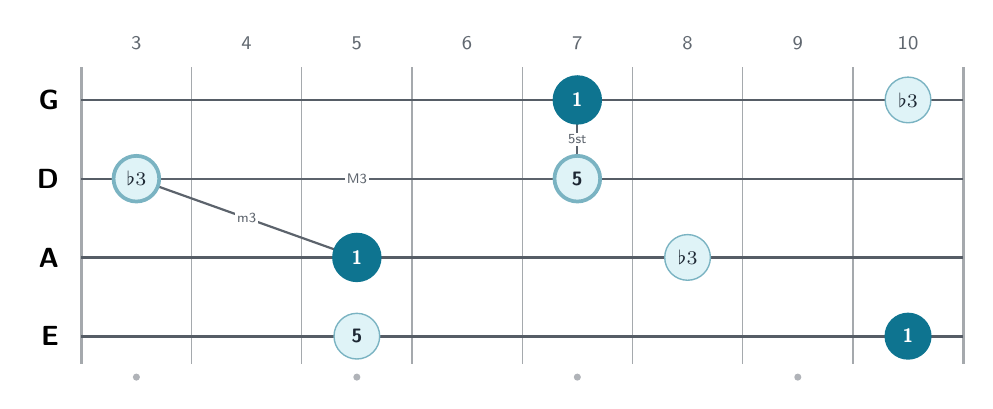
\begin{tikzpicture}[x=1cm,y=1cm,>=stealth]
\node[font=\sffamily\scriptsize,text=Ink!70] at (0.700,4.22) {3};
\node[font=\sffamily\scriptsize,text=Ink!70] at (2.100,4.22) {4};
\node[font=\sffamily\scriptsize,text=Ink!70] at (3.500,4.22) {5};
\node[font=\sffamily\scriptsize,text=Ink!70] at (4.900,4.22) {6};
\node[font=\sffamily\scriptsize,text=Ink!70] at (6.300,4.22) {7};
\node[font=\sffamily\scriptsize,text=Ink!70] at (7.700,4.22) {8};
\node[font=\sffamily\scriptsize,text=Ink!70] at (9.100,4.22) {9};
\node[font=\sffamily\scriptsize,text=Ink!70] at (10.500,4.22) {10};
\draw[Ink!40,line width=1.0pt] (0.000,0.15) -- (0.000,3.92);
\draw[Ink!40,line width=0.45pt] (1.400,0.15) -- (1.400,3.92);
\draw[Ink!40,line width=0.45pt] (2.800,0.15) -- (2.800,3.92);
\draw[Ink!40,line width=0.45pt] (4.200,0.15) -- (4.200,3.92);
\draw[Ink!40,line width=0.45pt] (5.600,0.15) -- (5.600,3.92);
\draw[Ink!40,line width=0.45pt] (7.000,0.15) -- (7.000,3.92);
\draw[Ink!40,line width=0.45pt] (8.400,0.15) -- (8.400,3.92);
\draw[Ink!40,line width=0.45pt] (9.800,0.15) -- (9.800,3.92);
\draw[Ink!40,line width=1.0pt] (11.200,0.15) -- (11.200,3.92);
\node[anchor=east,font=\sffamily\bfseries] at (-0.16,3.50) {G};
\draw[Ink!75,line width=0.45pt] (0,3.50) -- (11.200,3.50);
\node[anchor=east,font=\sffamily\bfseries] at (-0.16,2.50) {D};
\draw[Ink!75,line width=0.6pt] (0,2.50) -- (11.200,2.50);
\node[anchor=east,font=\sffamily\bfseries] at (-0.16,1.50) {A};
\draw[Ink!75,line width=0.8pt] (0,1.50) -- (11.200,1.50);
\node[anchor=east,font=\sffamily\bfseries] at (-0.16,0.50) {E};
\draw[Ink!75,line width=1.0pt] (0,0.50) -- (11.200,0.50);
\fill[Ink!35] (0.700,-0.02) circle (0.045);
\fill[Ink!35] (3.500,-0.02) circle (0.045);
\fill[Ink!35] (6.300,-0.02) circle (0.045);
\fill[Ink!35] (9.100,-0.02) circle (0.045);
\draw[->,Ink!72,line width=0.8pt] (3.500,1.500) -- node[midway,fill=white,inner sep=0.8pt,font=\sffamily\tiny] {m3} (0.700,2.500);
\draw[->,Ink!72,line width=0.8pt] (0.700,2.500) -- node[midway,fill=white,inner sep=0.8pt,font=\sffamily\tiny] {M3} (6.300,2.500);
\draw[->,Ink!72,line width=0.8pt] (6.300,2.500) -- node[midway,fill=white,inner sep=0.8pt,font=\sffamily\tiny] {5st} (6.300,3.500);
\node[circle,minimum size=0.58cm,inner sep=0pt,fill=Accent,draw=Accent,line width=1.35pt,font=\sffamily\bfseries\scriptsize,text=white] at (6.300,3.500) {1};
\node[circle,minimum size=0.58cm,inner sep=0pt,fill=AccentLight,draw=Accent!55,line width=0.5pt,font=\sffamily\bfseries\scriptsize,text=Ink] at (10.500,3.500) {$\flat3$};
\node[circle,minimum size=0.58cm,inner sep=0pt,fill=AccentLight,draw=Accent!55,line width=1.35pt,font=\sffamily\bfseries\scriptsize,text=Ink] at (0.700,2.500) {$\flat3$};
\node[circle,minimum size=0.58cm,inner sep=0pt,fill=AccentLight,draw=Accent!55,line width=1.35pt,font=\sffamily\bfseries\scriptsize,text=Ink] at (6.300,2.500) {5};
\node[circle,minimum size=0.58cm,inner sep=0pt,fill=Accent,draw=Accent,line width=1.35pt,font=\sffamily\bfseries\scriptsize,text=white] at (3.500,1.500) {1};
\node[circle,minimum size=0.58cm,inner sep=0pt,fill=AccentLight,draw=Accent!55,line width=0.5pt,font=\sffamily\bfseries\scriptsize,text=Ink] at (7.700,1.500) {$\flat3$};
\node[circle,minimum size=0.58cm,inner sep=0pt,fill=AccentLight,draw=Accent!55,line width=0.5pt,font=\sffamily\bfseries\scriptsize,text=Ink] at (3.500,0.500) {5};
\node[circle,minimum size=0.58cm,inner sep=0pt,fill=Accent,draw=Accent,line width=0.5pt,font=\sffamily\bfseries\scriptsize,text=white] at (10.500,0.500) {1};
\end{tikzpicture}
\end{center}
\clearpage
\subsection{Major seventh}
\begin{tabularx}{\textwidth}{>{\bfseries\sffamily}p{2.5cm}Y}
Formula & 1 3 5 7 \quad Example: D--F\#--A--C\#--D \quad Use: Major-7 harmony \\
\end{tabularx}
\begin{center}
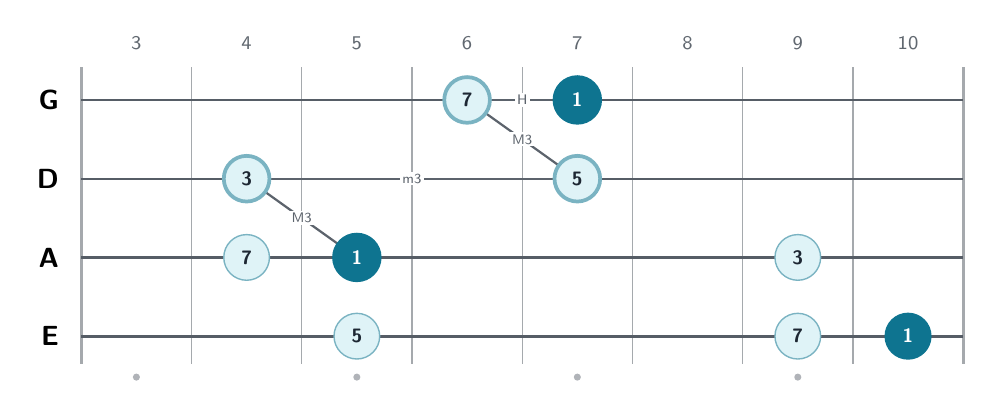
\begin{tikzpicture}[x=1cm,y=1cm,>=stealth]
\node[font=\sffamily\scriptsize,text=Ink!70] at (0.700,4.22) {3};
\node[font=\sffamily\scriptsize,text=Ink!70] at (2.100,4.22) {4};
\node[font=\sffamily\scriptsize,text=Ink!70] at (3.500,4.22) {5};
\node[font=\sffamily\scriptsize,text=Ink!70] at (4.900,4.22) {6};
\node[font=\sffamily\scriptsize,text=Ink!70] at (6.300,4.22) {7};
\node[font=\sffamily\scriptsize,text=Ink!70] at (7.700,4.22) {8};
\node[font=\sffamily\scriptsize,text=Ink!70] at (9.100,4.22) {9};
\node[font=\sffamily\scriptsize,text=Ink!70] at (10.500,4.22) {10};
\draw[Ink!40,line width=1.0pt] (0.000,0.15) -- (0.000,3.92);
\draw[Ink!40,line width=0.45pt] (1.400,0.15) -- (1.400,3.92);
\draw[Ink!40,line width=0.45pt] (2.800,0.15) -- (2.800,3.92);
\draw[Ink!40,line width=0.45pt] (4.200,0.15) -- (4.200,3.92);
\draw[Ink!40,line width=0.45pt] (5.600,0.15) -- (5.600,3.92);
\draw[Ink!40,line width=0.45pt] (7.000,0.15) -- (7.000,3.92);
\draw[Ink!40,line width=0.45pt] (8.400,0.15) -- (8.400,3.92);
\draw[Ink!40,line width=0.45pt] (9.800,0.15) -- (9.800,3.92);
\draw[Ink!40,line width=1.0pt] (11.200,0.15) -- (11.200,3.92);
\node[anchor=east,font=\sffamily\bfseries] at (-0.16,3.50) {G};
\draw[Ink!75,line width=0.45pt] (0,3.50) -- (11.200,3.50);
\node[anchor=east,font=\sffamily\bfseries] at (-0.16,2.50) {D};
\draw[Ink!75,line width=0.6pt] (0,2.50) -- (11.200,2.50);
\node[anchor=east,font=\sffamily\bfseries] at (-0.16,1.50) {A};
\draw[Ink!75,line width=0.8pt] (0,1.50) -- (11.200,1.50);
\node[anchor=east,font=\sffamily\bfseries] at (-0.16,0.50) {E};
\draw[Ink!75,line width=1.0pt] (0,0.50) -- (11.200,0.50);
\fill[Ink!35] (0.700,-0.02) circle (0.045);
\fill[Ink!35] (3.500,-0.02) circle (0.045);
\fill[Ink!35] (6.300,-0.02) circle (0.045);
\fill[Ink!35] (9.100,-0.02) circle (0.045);
\draw[->,Ink!72,line width=0.8pt] (3.500,1.500) -- node[midway,fill=white,inner sep=0.8pt,font=\sffamily\tiny] {M3} (2.100,2.500);
\draw[->,Ink!72,line width=0.8pt] (2.100,2.500) -- node[midway,fill=white,inner sep=0.8pt,font=\sffamily\tiny] {m3} (6.300,2.500);
\draw[->,Ink!72,line width=0.8pt] (6.300,2.500) -- node[midway,fill=white,inner sep=0.8pt,font=\sffamily\tiny] {M3} (4.900,3.500);
\draw[->,Ink!72,line width=0.8pt] (4.900,3.500) -- node[midway,fill=white,inner sep=0.8pt,font=\sffamily\tiny] {H} (6.300,3.500);
\node[circle,minimum size=0.58cm,inner sep=0pt,fill=AccentLight,draw=Accent!55,line width=1.35pt,font=\sffamily\bfseries\scriptsize,text=Ink] at (4.900,3.500) {7};
\node[circle,minimum size=0.58cm,inner sep=0pt,fill=Accent,draw=Accent,line width=1.35pt,font=\sffamily\bfseries\scriptsize,text=white] at (6.300,3.500) {1};
\node[circle,minimum size=0.58cm,inner sep=0pt,fill=AccentLight,draw=Accent!55,line width=1.35pt,font=\sffamily\bfseries\scriptsize,text=Ink] at (2.100,2.500) {3};
\node[circle,minimum size=0.58cm,inner sep=0pt,fill=AccentLight,draw=Accent!55,line width=1.35pt,font=\sffamily\bfseries\scriptsize,text=Ink] at (6.300,2.500) {5};
\node[circle,minimum size=0.58cm,inner sep=0pt,fill=AccentLight,draw=Accent!55,line width=0.5pt,font=\sffamily\bfseries\scriptsize,text=Ink] at (2.100,1.500) {7};
\node[circle,minimum size=0.58cm,inner sep=0pt,fill=Accent,draw=Accent,line width=1.35pt,font=\sffamily\bfseries\scriptsize,text=white] at (3.500,1.500) {1};
\node[circle,minimum size=0.58cm,inner sep=0pt,fill=AccentLight,draw=Accent!55,line width=0.5pt,font=\sffamily\bfseries\scriptsize,text=Ink] at (9.100,1.500) {3};
\node[circle,minimum size=0.58cm,inner sep=0pt,fill=AccentLight,draw=Accent!55,line width=0.5pt,font=\sffamily\bfseries\scriptsize,text=Ink] at (3.500,0.500) {5};
\node[circle,minimum size=0.58cm,inner sep=0pt,fill=AccentLight,draw=Accent!55,line width=0.5pt,font=\sffamily\bfseries\scriptsize,text=Ink] at (9.100,0.500) {7};
\node[circle,minimum size=0.58cm,inner sep=0pt,fill=Accent,draw=Accent,line width=0.5pt,font=\sffamily\bfseries\scriptsize,text=white] at (10.500,0.500) {1};
\end{tikzpicture}
\end{center}
\subsection{Dominant seventh}
\begin{tabularx}{\textwidth}{>{\bfseries\sffamily}p{2.5cm}Y}
Formula & 1 3 5 $\flat7$ \quad Example: D--F\#--A--C--D \quad Use: Dominant-7 harmony; strong resolution \\
\end{tabularx}
\begin{center}
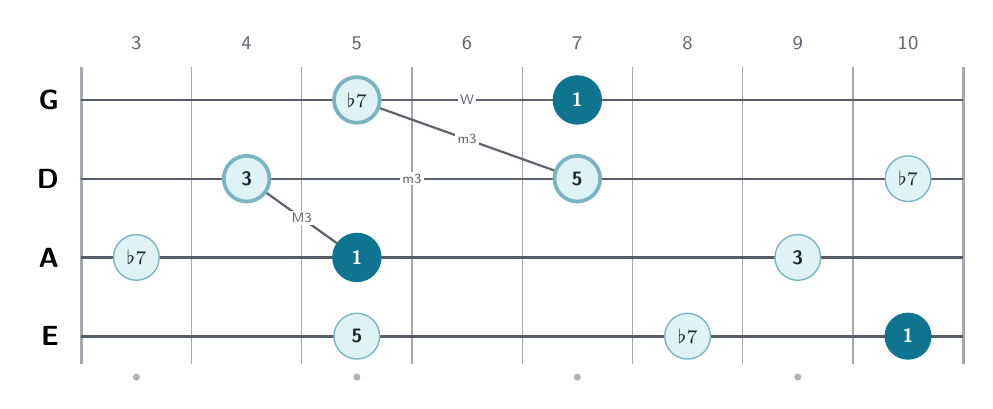
\begin{tikzpicture}[x=1cm,y=1cm,>=stealth]
\node[font=\sffamily\scriptsize,text=Ink!70] at (0.700,4.22) {3};
\node[font=\sffamily\scriptsize,text=Ink!70] at (2.100,4.22) {4};
\node[font=\sffamily\scriptsize,text=Ink!70] at (3.500,4.22) {5};
\node[font=\sffamily\scriptsize,text=Ink!70] at (4.900,4.22) {6};
\node[font=\sffamily\scriptsize,text=Ink!70] at (6.300,4.22) {7};
\node[font=\sffamily\scriptsize,text=Ink!70] at (7.700,4.22) {8};
\node[font=\sffamily\scriptsize,text=Ink!70] at (9.100,4.22) {9};
\node[font=\sffamily\scriptsize,text=Ink!70] at (10.500,4.22) {10};
\draw[Ink!40,line width=1.0pt] (0.000,0.15) -- (0.000,3.92);
\draw[Ink!40,line width=0.45pt] (1.400,0.15) -- (1.400,3.92);
\draw[Ink!40,line width=0.45pt] (2.800,0.15) -- (2.800,3.92);
\draw[Ink!40,line width=0.45pt] (4.200,0.15) -- (4.200,3.92);
\draw[Ink!40,line width=0.45pt] (5.600,0.15) -- (5.600,3.92);
\draw[Ink!40,line width=0.45pt] (7.000,0.15) -- (7.000,3.92);
\draw[Ink!40,line width=0.45pt] (8.400,0.15) -- (8.400,3.92);
\draw[Ink!40,line width=0.45pt] (9.800,0.15) -- (9.800,3.92);
\draw[Ink!40,line width=1.0pt] (11.200,0.15) -- (11.200,3.92);
\node[anchor=east,font=\sffamily\bfseries] at (-0.16,3.50) {G};
\draw[Ink!75,line width=0.45pt] (0,3.50) -- (11.200,3.50);
\node[anchor=east,font=\sffamily\bfseries] at (-0.16,2.50) {D};
\draw[Ink!75,line width=0.6pt] (0,2.50) -- (11.200,2.50);
\node[anchor=east,font=\sffamily\bfseries] at (-0.16,1.50) {A};
\draw[Ink!75,line width=0.8pt] (0,1.50) -- (11.200,1.50);
\node[anchor=east,font=\sffamily\bfseries] at (-0.16,0.50) {E};
\draw[Ink!75,line width=1.0pt] (0,0.50) -- (11.200,0.50);
\fill[Ink!35] (0.700,-0.02) circle (0.045);
\fill[Ink!35] (3.500,-0.02) circle (0.045);
\fill[Ink!35] (6.300,-0.02) circle (0.045);
\fill[Ink!35] (9.100,-0.02) circle (0.045);
\draw[->,Ink!72,line width=0.8pt] (3.500,1.500) -- node[midway,fill=white,inner sep=0.8pt,font=\sffamily\tiny] {M3} (2.100,2.500);
\draw[->,Ink!72,line width=0.8pt] (2.100,2.500) -- node[midway,fill=white,inner sep=0.8pt,font=\sffamily\tiny] {m3} (6.300,2.500);
\draw[->,Ink!72,line width=0.8pt] (6.300,2.500) -- node[midway,fill=white,inner sep=0.8pt,font=\sffamily\tiny] {m3} (3.500,3.500);
\draw[->,Ink!72,line width=0.8pt] (3.500,3.500) -- node[midway,fill=white,inner sep=0.8pt,font=\sffamily\tiny] {W} (6.300,3.500);
\node[circle,minimum size=0.58cm,inner sep=0pt,fill=AccentLight,draw=Accent!55,line width=1.35pt,font=\sffamily\bfseries\scriptsize,text=Ink] at (3.500,3.500) {$\flat7$};
\node[circle,minimum size=0.58cm,inner sep=0pt,fill=Accent,draw=Accent,line width=1.35pt,font=\sffamily\bfseries\scriptsize,text=white] at (6.300,3.500) {1};
\node[circle,minimum size=0.58cm,inner sep=0pt,fill=AccentLight,draw=Accent!55,line width=1.35pt,font=\sffamily\bfseries\scriptsize,text=Ink] at (2.100,2.500) {3};
\node[circle,minimum size=0.58cm,inner sep=0pt,fill=AccentLight,draw=Accent!55,line width=1.35pt,font=\sffamily\bfseries\scriptsize,text=Ink] at (6.300,2.500) {5};
\node[circle,minimum size=0.58cm,inner sep=0pt,fill=AccentLight,draw=Accent!55,line width=0.5pt,font=\sffamily\bfseries\scriptsize,text=Ink] at (10.500,2.500) {$\flat7$};
\node[circle,minimum size=0.58cm,inner sep=0pt,fill=AccentLight,draw=Accent!55,line width=0.5pt,font=\sffamily\bfseries\scriptsize,text=Ink] at (0.700,1.500) {$\flat7$};
\node[circle,minimum size=0.58cm,inner sep=0pt,fill=Accent,draw=Accent,line width=1.35pt,font=\sffamily\bfseries\scriptsize,text=white] at (3.500,1.500) {1};
\node[circle,minimum size=0.58cm,inner sep=0pt,fill=AccentLight,draw=Accent!55,line width=0.5pt,font=\sffamily\bfseries\scriptsize,text=Ink] at (9.100,1.500) {3};
\node[circle,minimum size=0.58cm,inner sep=0pt,fill=AccentLight,draw=Accent!55,line width=0.5pt,font=\sffamily\bfseries\scriptsize,text=Ink] at (3.500,0.500) {5};
\node[circle,minimum size=0.58cm,inner sep=0pt,fill=AccentLight,draw=Accent!55,line width=0.5pt,font=\sffamily\bfseries\scriptsize,text=Ink] at (7.700,0.500) {$\flat7$};
\node[circle,minimum size=0.58cm,inner sep=0pt,fill=Accent,draw=Accent,line width=0.5pt,font=\sffamily\bfseries\scriptsize,text=white] at (10.500,0.500) {1};
\end{tikzpicture}
\end{center}
\clearpage
\subsection{Minor seventh}
\begin{tabularx}{\textwidth}{>{\bfseries\sffamily}p{2.5cm}Y}
Formula & 1 $\flat3$ 5 $\flat7$ \quad Example: D--F--A--C--D \quad Use: Minor-7 harmony \\
\end{tabularx}
\begin{center}
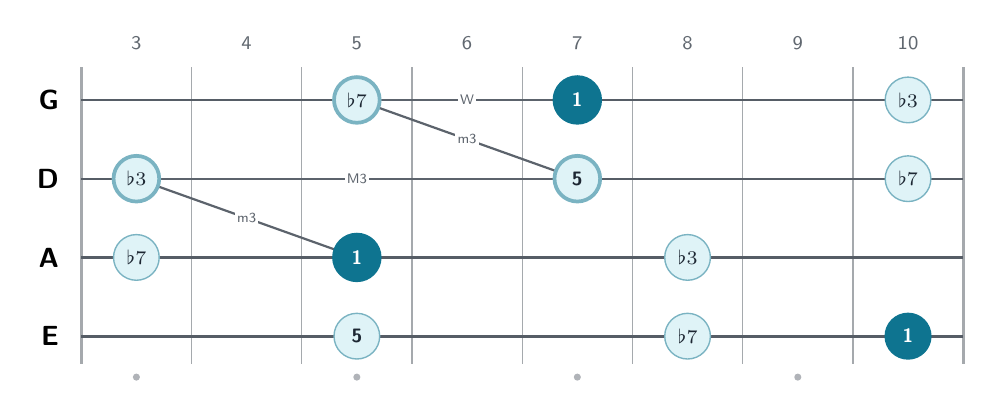
\begin{tikzpicture}[x=1cm,y=1cm,>=stealth]
\node[font=\sffamily\scriptsize,text=Ink!70] at (0.700,4.22) {3};
\node[font=\sffamily\scriptsize,text=Ink!70] at (2.100,4.22) {4};
\node[font=\sffamily\scriptsize,text=Ink!70] at (3.500,4.22) {5};
\node[font=\sffamily\scriptsize,text=Ink!70] at (4.900,4.22) {6};
\node[font=\sffamily\scriptsize,text=Ink!70] at (6.300,4.22) {7};
\node[font=\sffamily\scriptsize,text=Ink!70] at (7.700,4.22) {8};
\node[font=\sffamily\scriptsize,text=Ink!70] at (9.100,4.22) {9};
\node[font=\sffamily\scriptsize,text=Ink!70] at (10.500,4.22) {10};
\draw[Ink!40,line width=1.0pt] (0.000,0.15) -- (0.000,3.92);
\draw[Ink!40,line width=0.45pt] (1.400,0.15) -- (1.400,3.92);
\draw[Ink!40,line width=0.45pt] (2.800,0.15) -- (2.800,3.92);
\draw[Ink!40,line width=0.45pt] (4.200,0.15) -- (4.200,3.92);
\draw[Ink!40,line width=0.45pt] (5.600,0.15) -- (5.600,3.92);
\draw[Ink!40,line width=0.45pt] (7.000,0.15) -- (7.000,3.92);
\draw[Ink!40,line width=0.45pt] (8.400,0.15) -- (8.400,3.92);
\draw[Ink!40,line width=0.45pt] (9.800,0.15) -- (9.800,3.92);
\draw[Ink!40,line width=1.0pt] (11.200,0.15) -- (11.200,3.92);
\node[anchor=east,font=\sffamily\bfseries] at (-0.16,3.50) {G};
\draw[Ink!75,line width=0.45pt] (0,3.50) -- (11.200,3.50);
\node[anchor=east,font=\sffamily\bfseries] at (-0.16,2.50) {D};
\draw[Ink!75,line width=0.6pt] (0,2.50) -- (11.200,2.50);
\node[anchor=east,font=\sffamily\bfseries] at (-0.16,1.50) {A};
\draw[Ink!75,line width=0.8pt] (0,1.50) -- (11.200,1.50);
\node[anchor=east,font=\sffamily\bfseries] at (-0.16,0.50) {E};
\draw[Ink!75,line width=1.0pt] (0,0.50) -- (11.200,0.50);
\fill[Ink!35] (0.700,-0.02) circle (0.045);
\fill[Ink!35] (3.500,-0.02) circle (0.045);
\fill[Ink!35] (6.300,-0.02) circle (0.045);
\fill[Ink!35] (9.100,-0.02) circle (0.045);
\draw[->,Ink!72,line width=0.8pt] (3.500,1.500) -- node[midway,fill=white,inner sep=0.8pt,font=\sffamily\tiny] {m3} (0.700,2.500);
\draw[->,Ink!72,line width=0.8pt] (0.700,2.500) -- node[midway,fill=white,inner sep=0.8pt,font=\sffamily\tiny] {M3} (6.300,2.500);
\draw[->,Ink!72,line width=0.8pt] (6.300,2.500) -- node[midway,fill=white,inner sep=0.8pt,font=\sffamily\tiny] {m3} (3.500,3.500);
\draw[->,Ink!72,line width=0.8pt] (3.500,3.500) -- node[midway,fill=white,inner sep=0.8pt,font=\sffamily\tiny] {W} (6.300,3.500);
\node[circle,minimum size=0.58cm,inner sep=0pt,fill=AccentLight,draw=Accent!55,line width=1.35pt,font=\sffamily\bfseries\scriptsize,text=Ink] at (3.500,3.500) {$\flat7$};
\node[circle,minimum size=0.58cm,inner sep=0pt,fill=Accent,draw=Accent,line width=1.35pt,font=\sffamily\bfseries\scriptsize,text=white] at (6.300,3.500) {1};
\node[circle,minimum size=0.58cm,inner sep=0pt,fill=AccentLight,draw=Accent!55,line width=0.5pt,font=\sffamily\bfseries\scriptsize,text=Ink] at (10.500,3.500) {$\flat3$};
\node[circle,minimum size=0.58cm,inner sep=0pt,fill=AccentLight,draw=Accent!55,line width=1.35pt,font=\sffamily\bfseries\scriptsize,text=Ink] at (0.700,2.500) {$\flat3$};
\node[circle,minimum size=0.58cm,inner sep=0pt,fill=AccentLight,draw=Accent!55,line width=1.35pt,font=\sffamily\bfseries\scriptsize,text=Ink] at (6.300,2.500) {5};
\node[circle,minimum size=0.58cm,inner sep=0pt,fill=AccentLight,draw=Accent!55,line width=0.5pt,font=\sffamily\bfseries\scriptsize,text=Ink] at (10.500,2.500) {$\flat7$};
\node[circle,minimum size=0.58cm,inner sep=0pt,fill=AccentLight,draw=Accent!55,line width=0.5pt,font=\sffamily\bfseries\scriptsize,text=Ink] at (0.700,1.500) {$\flat7$};
\node[circle,minimum size=0.58cm,inner sep=0pt,fill=Accent,draw=Accent,line width=1.35pt,font=\sffamily\bfseries\scriptsize,text=white] at (3.500,1.500) {1};
\node[circle,minimum size=0.58cm,inner sep=0pt,fill=AccentLight,draw=Accent!55,line width=0.5pt,font=\sffamily\bfseries\scriptsize,text=Ink] at (7.700,1.500) {$\flat3$};
\node[circle,minimum size=0.58cm,inner sep=0pt,fill=AccentLight,draw=Accent!55,line width=0.5pt,font=\sffamily\bfseries\scriptsize,text=Ink] at (3.500,0.500) {5};
\node[circle,minimum size=0.58cm,inner sep=0pt,fill=AccentLight,draw=Accent!55,line width=0.5pt,font=\sffamily\bfseries\scriptsize,text=Ink] at (7.700,0.500) {$\flat7$};
\node[circle,minimum size=0.58cm,inner sep=0pt,fill=Accent,draw=Accent,line width=0.5pt,font=\sffamily\bfseries\scriptsize,text=white] at (10.500,0.500) {1};
\end{tikzpicture}
\end{center}
\subsection{Half-diminished}
\begin{tabularx}{\textwidth}{>{\bfseries\sffamily}p{2.5cm}Y}
Formula & 1 $\flat3$ $\flat5$ $\flat7$ \quad Example: D--F--A$\flat$--C--D \quad Use: Minor-7-flat-5 harmony \\
\end{tabularx}
\begin{center}
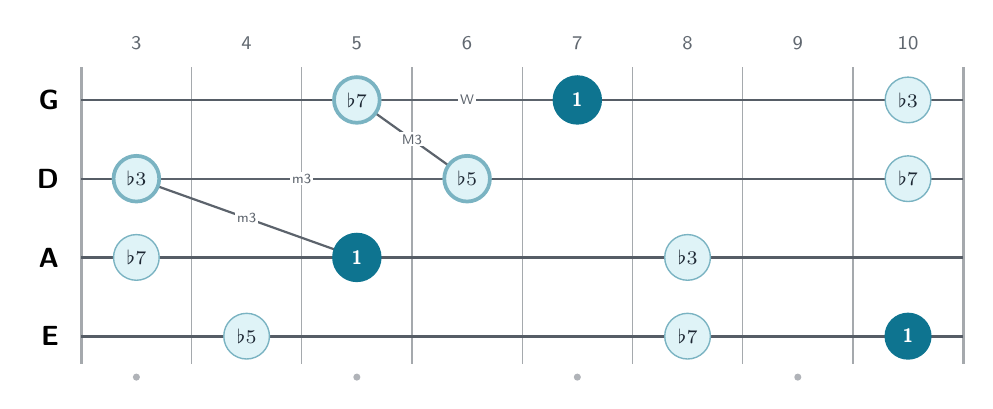
\begin{tikzpicture}[x=1cm,y=1cm,>=stealth]
\node[font=\sffamily\scriptsize,text=Ink!70] at (0.700,4.22) {3};
\node[font=\sffamily\scriptsize,text=Ink!70] at (2.100,4.22) {4};
\node[font=\sffamily\scriptsize,text=Ink!70] at (3.500,4.22) {5};
\node[font=\sffamily\scriptsize,text=Ink!70] at (4.900,4.22) {6};
\node[font=\sffamily\scriptsize,text=Ink!70] at (6.300,4.22) {7};
\node[font=\sffamily\scriptsize,text=Ink!70] at (7.700,4.22) {8};
\node[font=\sffamily\scriptsize,text=Ink!70] at (9.100,4.22) {9};
\node[font=\sffamily\scriptsize,text=Ink!70] at (10.500,4.22) {10};
\draw[Ink!40,line width=1.0pt] (0.000,0.15) -- (0.000,3.92);
\draw[Ink!40,line width=0.45pt] (1.400,0.15) -- (1.400,3.92);
\draw[Ink!40,line width=0.45pt] (2.800,0.15) -- (2.800,3.92);
\draw[Ink!40,line width=0.45pt] (4.200,0.15) -- (4.200,3.92);
\draw[Ink!40,line width=0.45pt] (5.600,0.15) -- (5.600,3.92);
\draw[Ink!40,line width=0.45pt] (7.000,0.15) -- (7.000,3.92);
\draw[Ink!40,line width=0.45pt] (8.400,0.15) -- (8.400,3.92);
\draw[Ink!40,line width=0.45pt] (9.800,0.15) -- (9.800,3.92);
\draw[Ink!40,line width=1.0pt] (11.200,0.15) -- (11.200,3.92);
\node[anchor=east,font=\sffamily\bfseries] at (-0.16,3.50) {G};
\draw[Ink!75,line width=0.45pt] (0,3.50) -- (11.200,3.50);
\node[anchor=east,font=\sffamily\bfseries] at (-0.16,2.50) {D};
\draw[Ink!75,line width=0.6pt] (0,2.50) -- (11.200,2.50);
\node[anchor=east,font=\sffamily\bfseries] at (-0.16,1.50) {A};
\draw[Ink!75,line width=0.8pt] (0,1.50) -- (11.200,1.50);
\node[anchor=east,font=\sffamily\bfseries] at (-0.16,0.50) {E};
\draw[Ink!75,line width=1.0pt] (0,0.50) -- (11.200,0.50);
\fill[Ink!35] (0.700,-0.02) circle (0.045);
\fill[Ink!35] (3.500,-0.02) circle (0.045);
\fill[Ink!35] (6.300,-0.02) circle (0.045);
\fill[Ink!35] (9.100,-0.02) circle (0.045);
\draw[->,Ink!72,line width=0.8pt] (3.500,1.500) -- node[midway,fill=white,inner sep=0.8pt,font=\sffamily\tiny] {m3} (0.700,2.500);
\draw[->,Ink!72,line width=0.8pt] (0.700,2.500) -- node[midway,fill=white,inner sep=0.8pt,font=\sffamily\tiny] {m3} (4.900,2.500);
\draw[->,Ink!72,line width=0.8pt] (4.900,2.500) -- node[midway,fill=white,inner sep=0.8pt,font=\sffamily\tiny] {M3} (3.500,3.500);
\draw[->,Ink!72,line width=0.8pt] (3.500,3.500) -- node[midway,fill=white,inner sep=0.8pt,font=\sffamily\tiny] {W} (6.300,3.500);
\node[circle,minimum size=0.58cm,inner sep=0pt,fill=AccentLight,draw=Accent!55,line width=1.35pt,font=\sffamily\bfseries\scriptsize,text=Ink] at (3.500,3.500) {$\flat7$};
\node[circle,minimum size=0.58cm,inner sep=0pt,fill=Accent,draw=Accent,line width=1.35pt,font=\sffamily\bfseries\scriptsize,text=white] at (6.300,3.500) {1};
\node[circle,minimum size=0.58cm,inner sep=0pt,fill=AccentLight,draw=Accent!55,line width=0.5pt,font=\sffamily\bfseries\scriptsize,text=Ink] at (10.500,3.500) {$\flat3$};
\node[circle,minimum size=0.58cm,inner sep=0pt,fill=AccentLight,draw=Accent!55,line width=1.35pt,font=\sffamily\bfseries\scriptsize,text=Ink] at (0.700,2.500) {$\flat3$};
\node[circle,minimum size=0.58cm,inner sep=0pt,fill=AccentLight,draw=Accent!55,line width=1.35pt,font=\sffamily\bfseries\scriptsize,text=Ink] at (4.900,2.500) {$\flat5$};
\node[circle,minimum size=0.58cm,inner sep=0pt,fill=AccentLight,draw=Accent!55,line width=0.5pt,font=\sffamily\bfseries\scriptsize,text=Ink] at (10.500,2.500) {$\flat7$};
\node[circle,minimum size=0.58cm,inner sep=0pt,fill=AccentLight,draw=Accent!55,line width=0.5pt,font=\sffamily\bfseries\scriptsize,text=Ink] at (0.700,1.500) {$\flat7$};
\node[circle,minimum size=0.58cm,inner sep=0pt,fill=Accent,draw=Accent,line width=1.35pt,font=\sffamily\bfseries\scriptsize,text=white] at (3.500,1.500) {1};
\node[circle,minimum size=0.58cm,inner sep=0pt,fill=AccentLight,draw=Accent!55,line width=0.5pt,font=\sffamily\bfseries\scriptsize,text=Ink] at (7.700,1.500) {$\flat3$};
\node[circle,minimum size=0.58cm,inner sep=0pt,fill=AccentLight,draw=Accent!55,line width=0.5pt,font=\sffamily\bfseries\scriptsize,text=Ink] at (2.100,0.500) {$\flat5$};
\node[circle,minimum size=0.58cm,inner sep=0pt,fill=AccentLight,draw=Accent!55,line width=0.5pt,font=\sffamily\bfseries\scriptsize,text=Ink] at (7.700,0.500) {$\flat7$};
\node[circle,minimum size=0.58cm,inner sep=0pt,fill=Accent,draw=Accent,line width=0.5pt,font=\sffamily\bfseries\scriptsize,text=white] at (10.500,0.500) {1};
\end{tikzpicture}
\end{center}
\clearpage
\section{How to build a basic bassline}
\begin{greenbox}
A basic bassline can be built in layers: \textbf{rhythm first, roots second, chord tones third, approaches last}. Each added note should clarify the harmony or improve the connection to the next chord.
\end{greenbox}

\subsection{Layer 1: map the harmony}
For every chord, write its root and chord tones. Example progression:
\begin{center}
\begin{tabular}{C{3.4cm}C{3.4cm}C{3.4cm}C{3.4cm}}
\toprule
C & Am & F & G7 \\
\midrule
C--E--G & A--C--E & F--A--C & G--B--D--F \\
1--3--5 & 1--$\flat3$--5 & 1--3--5 & 1--3--5--$\flat7$ \\
\bottomrule
\end{tabular}
\end{center}

\subsection{Layer 2: place the roots}
Put the root on the strongest structural point, normally beat 1 in a simple 4/4 line:
\begin{center}
\begin{tabular}{C{3.4cm}C{3.4cm}C{3.4cm}C{3.4cm}}
\toprule
C & Am & F & G7 \\
\midrule
\textbf{C} -- -- -- & \textbf{A} -- -- -- & \textbf{F} -- -- -- & \textbf{G} -- -- -- \\
\bottomrule
\end{tabular}
\end{center}

\subsection{Layer 3: add stable chord tones}
Fifths are neutral and strong; thirds state major versus minor; sevenths define seventh chords. One quarter-note skeleton is:
\begin{center}
\begin{tabular}{C{3.4cm}C{3.4cm}C{3.4cm}C{3.4cm}}
\toprule
C & Am & F & G7 \\
\midrule
C -- G -- E -- G & A -- E -- C -- E & F -- C -- A -- C & G -- D -- F -- D \\
1 -- 5 -- 3 -- 5 & 1 -- 5 -- $\flat3$ -- 5 & 1 -- 5 -- 3 -- 5 & 1 -- 5 -- $\flat7$ -- 5 \\
\bottomrule
\end{tabular}
\end{center}

\subsection{Layer 4: connect the next root}
On the final subdivision before a chord change, approach the next root from a scale tone or from one fret above/below. The destination note is more important than whether the approach is diatonic or chromatic.

\begin{center}
\begin{tabular}{C{3.4cm}C{3.4cm}C{3.4cm}C{3.4cm}}
\toprule
C & Am & F & G7 \\
\midrule
C -- G -- E -- \textbf{B} & A -- E -- C -- \textbf{E} & F -- C -- A -- \textbf{F\#} & G -- D -- F -- \textbf{B} \\
R -- 5 -- 3 -- approach & R -- 5 -- $\flat3$ -- approach & R -- 5 -- 3 -- chromatic & R -- 5 -- $\flat7$ -- leading tone \\
$\searrow$ A & $\nearrow$ F & $\nearrow$ G & $\nearrow$ C \\
\bottomrule
\end{tabular}
\end{center}

\subsection{Layer 5: choose rhythm and note length}
The same pitch sequence can produce different basslines. Decide whether notes are short, sustained, tied, syncopated or anticipated. Repetition creates identity; small changes at the end of a phrase create direction.

\begin{tabularx}{\textwidth}{>{\bfseries\sffamily}p{3.2cm}Y}
\toprule
Element & Reference principle \\
\midrule
Root & Establishes the chord and tonal center. \\
Third & States major or minor; use deliberately because it strongly colours the line. \\
Fifth & Stable support that does not compete with the chord quality. \\
Seventh & Defines major-7, dominant-7 or minor-7 harmony. \\
Scale tone & Adds melodic connection while remaining inside the key or chord-scale. \\
Chromatic approach & One fret above or below a destination chord tone; tension resolves on arrival. \\
Octave & Reinforces the root with more motion and register contrast. \\
Rest / sustain & Controls groove as strongly as pitch choice. \\
\bottomrule
\end{tabularx}

\begin{keybox}
\textbf{Compact formula:} choose a rhythm $\rightarrow$ place the root $\rightarrow$ add one or two chord tones $\rightarrow$ approach the next root $\rightarrow$ repeat the cell with minimal variation.
\end{keybox}
\clearpage
\section{Bassline reference for salsa and Latin harmony}
\begin{neutralbox}
The harmonic construction method does not change: identify the chord, prioritize chord tones, and connect to the next harmony. What changes is the rhythmic placement and interaction with percussion.
\end{neutralbox}

\begin{tabularx}{\textwidth}{>{\bfseries\sffamily}p{3.2cm}Y}
\toprule
Reference point & Application \\
\midrule
Repeated cell & A tumbao is usually recognized by a stable repeating rhythmic-harmonic cell rather than by constant melodic variation. \\
Anticipation & The next root or another chord tone may arrive before the written downbeat and continue across it. \\
Chord tones & Root and fifth provide stability; third, sixth and seventh identify the exact harmony. \\
Dominant harmony & Mixolydian and dominant-7 arpeggios expose 3 and $\flat7$, the defining tritone of a dominant chord. \\
Minor harmony & Dorian supplies natural 6; natural minor supplies $\flat6$; use the form present in the actual chord or melody. \\
Minor-key cadence & Harmonic minor explains the raised 7 and the major-third dominant chord leading back to a minor tonic. \\
Chromatic connection & A one-fret approach into the anticipated destination is often more useful than running the complete scale. \\
Space & Sustains and rests leave room for conga, timbales, piano and vocals. \\
\bottomrule
\end{tabularx}

\section{Chord-to-scale lookup}
\begin{longtable}{>{\bfseries}p{3.4cm}p{4.2cm}p{4.0cm}p{4.0cm}}
\toprule
Chord / context & First reference & Important degrees & Alternatives / caution \\
\midrule
\endhead
Major triad & Major, major pentatonic & 1, 3, 5, 6 & Lydian when $\sharp4$ is supported \\
Major 7 & Major & 1, 3, 5, 7 & Lydian for maj7$\sharp11$ \\
Dominant 7 & Mixolydian & 1, 3, 5, $\flat7$ & Altered options depend on extensions and resolution \\
Minor triad & Natural minor or minor pentatonic & 1, $\flat3$, 5 & Check whether 6 is natural or flat \\
Minor 7 & Dorian or natural minor & 1, $\flat3$, 5, $\flat7$ & Dorian = 6; Aeolian = $\flat6$ \\
Minor-major 7 & Melodic minor & 1, $\flat3$, 5, 7 & Strong tonic-minor colour \\
Half-diminished & Locrian & 1, $\flat3$, $\flat5$, $\flat7$ & Locrian natural 2 may appear in some minor-key contexts \\
Minor V7--i cadence & Harmonic minor around the key center & $\flat3$, $\flat6$, 7 & The V chord itself is dominant; target its 3 and $\flat7$ \\
Blues / dominant vamp & Minor pentatonic, blues, Mixolydian & 1, $\flat3$/3, 5, $\flat7$ & Major and minor thirds can coexist stylistically \\
\bottomrule
\end{longtable}

\section{Compact formula sheet}
\begin{multicols}{2}
\begin{tabular}{>{\bfseries}l l}
Major & 1 2 3 4 5 6 7 \\
Natural minor & 1 2 $\flat3$ 4 5 $\flat6$ $\flat7$ \\
Dorian & 1 2 $\flat3$ 4 5 6 $\flat7$ \\
Phrygian & 1 $\flat2$ $\flat3$ 4 5 $\flat6$ $\flat7$ \\
Lydian & 1 2 3 $\sharp4$ 5 6 7 \\
Mixolydian & 1 2 3 4 5 6 $\flat7$ \\
Locrian & 1 $\flat2$ $\flat3$ 4 $\flat5$ $\flat6$ $\flat7$ \\
\end{tabular}

\columnbreak
\begin{tabular}{>{\bfseries}l l}
Harmonic minor & 1 2 $\flat3$ 4 5 $\flat6$ 7 \\
Melodic minor & 1 2 $\flat3$ 4 5 6 7 \\
Major pentatonic & 1 2 3 5 6 \\
Minor pentatonic & 1 $\flat3$ 4 5 $\flat7$ \\
Blues & 1 $\flat3$ 4 $\flat5$ 5 $\flat7$ \\
Major triad & 1 3 5 \\
Minor triad & 1 $\flat3$ 5 \\
Dominant 7 & 1 3 5 $\flat7$ \\
Minor 7 & 1 $\flat3$ 5 $\flat7$ \\
\end{tabular}
\end{multicols}


\clearpage
\section{Complete five-minute exercise library}
\begin{greenbox}
Every exercise is an independent five-minute block. Each page contains the same three views: the notes on the fretboard, standard bass-clef notation, and matching four-line bass TAB. The physical library develops control of the instrument; the musical library develops hearing, harmony, rhythm and usable bass vocabulary.
\end{greenbox}
\begin{tabularx}{\textwidth}{>{\bfseries\sffamily}p{3.3cm}Y}
Five-minute method & Spend roughly 30 seconds reading the three representations, four minutes looping the material, and 30 seconds recording the clean tempo and one problem. \\
Tempo rule & Begin slowly enough to remain relaxed. Add 4 bpm after three clean repetitions. Accuracy, muting and pulse take priority over speed. \\
Transposition & After the written pattern is secure, move it to another root while preserving intervals and rhythm. \\
Musical standard & A note is not complete until its start, duration and release are all controlled. \\
\end{tabularx}

\subsection*{Physical library index}
\begin{longtable}{>{\bfseries\sffamily}p{1.4cm}p{11.2cm}C{2.2cm}}
\toprule
ID & Five-minute block & Page \\
\midrule
\endhead
P1 & 1-2-3-4 chromatic cell & p.~\pageref{ex:p1} \\
P2 & 4-3-2-1 reverse cell & p.~\pageref{ex:p2} \\
P3 & Permutation 1-3-2-4 & p.~\pageref{ex:p3} \\
P4 & Permutation 1-4-2-3 & p.~\pageref{ex:p4} \\
P5 & Same-fret string ladder & p.~\pageref{ex:p5} \\
P6 & Diagonal spider outward & p.~\pageref{ex:p6} \\
P7 & Diagonal spider inward & p.~\pageref{ex:p7} \\
P8 & String-skipping ladder & p.~\pageref{ex:p8} \\
P9 & Two-fret position shift & p.~\pageref{ex:p9} \\
P10 & Whole-position string shift & p.~\pageref{ex:p10} \\
P11 & Movable octave shapes & p.~\pageref{ex:p11} \\
P12 & Root-fifth-octave triangle & p.~\pageref{ex:p12} \\
P13 & Minor-third and major-third control & p.~\pageref{ex:p13} \\
P14 & One-fret diagonal crawl & p.~\pageref{ex:p14} \\
P15 & Three-notes-per-string coordination & p.~\pageref{ex:p15} \\
P16 & Repeated-note plucking alternation & p.~\pageref{ex:p16} \\
P17 & Two-string alternation & p.~\pageref{ex:p17} \\
P18 & Wide string-skip control & p.~\pageref{ex:p18} \\
P19 & Hammer-on and pull-off cell & p.~\pageref{ex:p19} \\
P20 & Four-string endurance pedal & p.~\pageref{ex:p20} \\
\bottomrule
\end{longtable}
\subsection*{Musical library index}
\begin{longtable}{>{\bfseries\sffamily}p{1.4cm}p{11.2cm}C{2.2cm}}
\toprule
ID & Five-minute block & Page \\
\midrule
\endhead
M1 & D major scale & p.~\pageref{ex:m1} \\
M2 & D natural minor scale & p.~\pageref{ex:m2} \\
M3 & D major-pentatonic phrase & p.~\pageref{ex:m3} \\
M4 & D minor-pentatonic phrase & p.~\pageref{ex:m4} \\
M5 & D blues-scale phrase & p.~\pageref{ex:m5} \\
M6 & D major triad & p.~\pageref{ex:m6} \\
M7 & D minor triad & p.~\pageref{ex:m7} \\
M8 & D dominant-seven arpeggio & p.~\pageref{ex:m8} \\
M9 & D minor-seven arpeggio & p.~\pageref{ex:m9} \\
M10 & I-IV-V-I root-fifth line & p.~\pageref{ex:m10} \\
M11 & I-vi-ii-V root-third targeting & p.~\pageref{ex:m11} \\
M12 & ii-V-I seventh-chord chain in C & p.~\pageref{ex:m12} \\
M13 & D-major scale in thirds & p.~\pageref{ex:m13} \\
M14 & Chromatic approaches from below & p.~\pageref{ex:m14} \\
M15 & Chromatic approaches from above & p.~\pageref{ex:m15} \\
M16 & Two-sided enclosures & p.~\pageref{ex:m16} \\
M17 & D pedal-tone groove & p.~\pageref{ex:m17} \\
M18 & Syncopated D-minor groove & p.~\pageref{ex:m18} \\
M19 & Basic Latin two-hit cell & p.~\pageref{ex:m19} \\
M20 & Latin ii-V-I-VI turnaround & p.~\pageref{ex:m20} \\
\bottomrule
\end{longtable}
\clearpage
\section{Physical technique: 20 five-minute blocks}
\subsection{P1 - 1-2-3-4 chromatic cell}\label{ex:p1}
\begin{keybox}
\textbf{Five-minute block.} Quarter note = 50--100 bpm; eighth notes.\\
\textbf{Play:} Use fingers 1--2--3--4, then return 4--3--2--1. Repeat on every string.
\end{keybox}
\begin{center}
{\sffamily\bfseries\small Fretboard}\par\vspace{1mm}
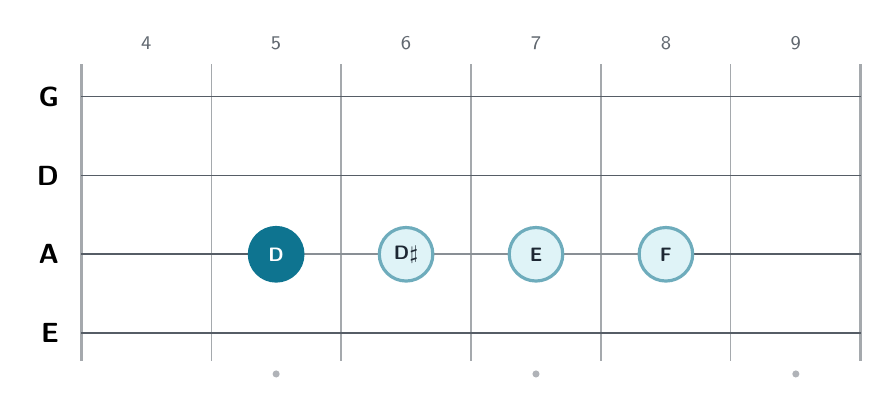
\begin{tikzpicture}[x=1cm,y=1cm,>=stealth]
\node[font=\sffamily\scriptsize,text=Ink!70] at (0.825,4.18) {4};
\node[font=\sffamily\scriptsize,text=Ink!70] at (2.475,4.18) {5};
\node[font=\sffamily\scriptsize,text=Ink!70] at (4.125,4.18) {6};
\node[font=\sffamily\scriptsize,text=Ink!70] at (5.775,4.18) {7};
\node[font=\sffamily\scriptsize,text=Ink!70] at (7.425,4.18) {8};
\node[font=\sffamily\scriptsize,text=Ink!70] at (9.075,4.18) {9};
\draw[Ink!40,line width=1.0pt] (0.000,0.15) -- (0.000,3.92);
\draw[Ink!40,line width=0.45pt] (1.650,0.15) -- (1.650,3.92);
\draw[Ink!40,line width=0.45pt] (3.300,0.15) -- (3.300,3.92);
\draw[Ink!40,line width=0.45pt] (4.950,0.15) -- (4.950,3.92);
\draw[Ink!40,line width=0.45pt] (6.600,0.15) -- (6.600,3.92);
\draw[Ink!40,line width=0.45pt] (8.250,0.15) -- (8.250,3.92);
\draw[Ink!40,line width=1.0pt] (9.900,0.15) -- (9.900,3.92);
\node[anchor=east,font=\sffamily\bfseries] at (-0.16,3.50) {G};
\draw[Ink!75,line width=0.45pt] (0,3.50) -- (9.900,3.50);
\node[anchor=east,font=\sffamily\bfseries] at (-0.16,2.50) {D};
\draw[Ink!75,line width=0.6pt] (0,2.50) -- (9.900,2.50);
\node[anchor=east,font=\sffamily\bfseries] at (-0.16,1.50) {A};
\draw[Ink!75,line width=0.8pt] (0,1.50) -- (9.900,1.50);
\node[anchor=east,font=\sffamily\bfseries] at (-0.16,0.50) {E};
\draw[Ink!75,line width=1.0pt] (0,0.50) -- (9.900,0.50);
\fill[Ink!35] (2.475,-0.02) circle (0.045);
\fill[Ink!35] (5.775,-0.02) circle (0.045);
\fill[Ink!35] (9.075,-0.02) circle (0.045);
\draw[->,Ink!52,line width=0.65pt] (2.475,1.500) -- (4.125,1.500);
\draw[->,Ink!52,line width=0.65pt] (4.125,1.500) -- (5.775,1.500);
\draw[->,Ink!52,line width=0.65pt] (5.775,1.500) -- (7.425,1.500);
\node[circle,minimum size=0.68cm,inner sep=0pt,fill=Accent,draw=Accent,text=white,line width=1.15pt,font=\sffamily\bfseries\scriptsize] at (2.475,1.500) {D};
\node[circle,minimum size=0.68cm,inner sep=0pt,fill=AccentLight,draw=Accent!60,text=Ink,line width=1.15pt,font=\sffamily\bfseries\scriptsize] at (4.125,1.500) {D$\sharp$};
\node[circle,minimum size=0.68cm,inner sep=0pt,fill=AccentLight,draw=Accent!60,text=Ink,line width=1.15pt,font=\sffamily\bfseries\scriptsize] at (5.775,1.500) {E};
\node[circle,minimum size=0.68cm,inner sep=0pt,fill=AccentLight,draw=Accent!60,text=Ink,line width=1.15pt,font=\sffamily\bfseries\scriptsize] at (7.425,1.500) {F};
\end{tikzpicture}
\end{center}
\begin{center}
\begingroup
\setlength{\parindent}{0pt}
\begin{minipage}{0.88\textwidth}
{\sffamily\bfseries\small Standard notation}\par\vspace{-1mm}
\begin{music}
\instrumentnumber{1}
\setstaffs1{1}
\setclef1{\bass}
\generalmeter{\meterfrac44}
\nobarnumbers
\nostartrule
\startextract
\Notes\cu{K}\cu{^K}\cu{L}\cu{M}\cu{M}\cu{L}\cu{K}\cu{=K}\en
\zendextract
\end{music}
\end{minipage}
\endgroup
\end{center}
\begin{center}
\begingroup
{\sffamily\bfseries\small Bass TAB}\par\vspace{1mm}
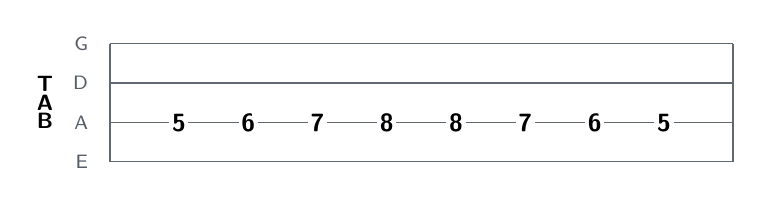
\begin{tikzpicture}[x=1cm,y=0.50cm]
\node[font=\sffamily\bfseries\footnotesize,align=center] at (-0.82,1.50) {T\\[-1mm]A\\[-1mm]B};
\foreach \y/\s in {3/G,2/D,1/A,0/E} {\draw[Ink!70,line width=0.55pt] (0,\y) -- (7.920,\y); \node[anchor=east,font=\sffamily\scriptsize,text=Ink!75] at (-0.15,\y) {\s};}
\draw[Ink!70,line width=0.7pt] (0,0) -- (0,3);
\draw[Ink!70,line width=0.7pt] (7.920,0) -- (7.920,3);
\node[fill=white,inner sep=1.0pt,font=\sffamily\bfseries\small] at (0.880,1) {5};
\node[fill=white,inner sep=1.0pt,font=\sffamily\bfseries\small] at (1.760,1) {6};
\node[fill=white,inner sep=1.0pt,font=\sffamily\bfseries\small] at (2.640,1) {7};
\node[fill=white,inner sep=1.0pt,font=\sffamily\bfseries\small] at (3.520,1) {8};
\node[fill=white,inner sep=1.0pt,font=\sffamily\bfseries\small] at (4.400,1) {8};
\node[fill=white,inner sep=1.0pt,font=\sffamily\bfseries\small] at (5.280,1) {7};
\node[fill=white,inner sep=1.0pt,font=\sffamily\bfseries\small] at (6.160,1) {6};
\node[fill=white,inner sep=1.0pt,font=\sffamily\bfseries\small] at (7.040,1) {5};
\end{tikzpicture}
\endgroup
\end{center}
\begin{tabularx}{\textwidth}{>{\bfseries\sffamily}p{3.0cm}Y}
Target & Equal attacks and minimum left-hand motion. \\
Progression & Begin at the lower tempo. Add 4 bpm after three clean repetitions; reduce by 6--8 bpm when timing or muting breaks down. \\
\end{tabularx}
\clearpage
\subsection{P2 - 4-3-2-1 reverse cell}\label{ex:p2}
\begin{keybox}
\textbf{Five-minute block.} Quarter note = 50--100 bpm; eighth notes.\\
\textbf{Play:} Begin with finger 4 and descend. Keep all unused fingers close to the string.
\end{keybox}
\begin{center}
{\sffamily\bfseries\small Fretboard}\par\vspace{1mm}
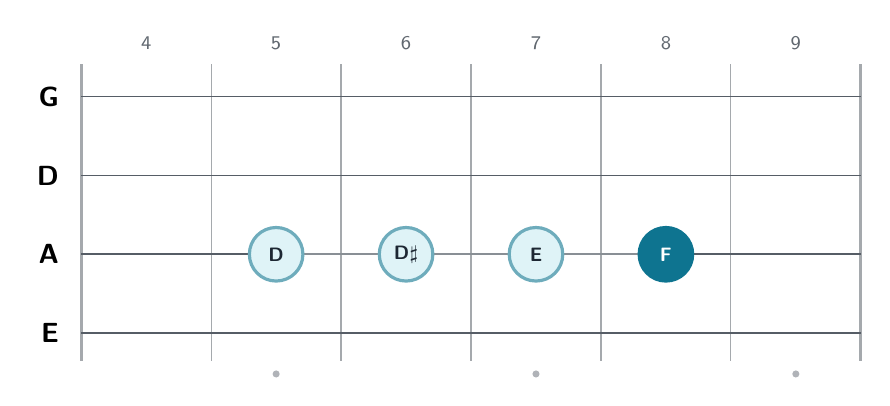
\begin{tikzpicture}[x=1cm,y=1cm,>=stealth]
\node[font=\sffamily\scriptsize,text=Ink!70] at (0.825,4.18) {4};
\node[font=\sffamily\scriptsize,text=Ink!70] at (2.475,4.18) {5};
\node[font=\sffamily\scriptsize,text=Ink!70] at (4.125,4.18) {6};
\node[font=\sffamily\scriptsize,text=Ink!70] at (5.775,4.18) {7};
\node[font=\sffamily\scriptsize,text=Ink!70] at (7.425,4.18) {8};
\node[font=\sffamily\scriptsize,text=Ink!70] at (9.075,4.18) {9};
\draw[Ink!40,line width=1.0pt] (0.000,0.15) -- (0.000,3.92);
\draw[Ink!40,line width=0.45pt] (1.650,0.15) -- (1.650,3.92);
\draw[Ink!40,line width=0.45pt] (3.300,0.15) -- (3.300,3.92);
\draw[Ink!40,line width=0.45pt] (4.950,0.15) -- (4.950,3.92);
\draw[Ink!40,line width=0.45pt] (6.600,0.15) -- (6.600,3.92);
\draw[Ink!40,line width=0.45pt] (8.250,0.15) -- (8.250,3.92);
\draw[Ink!40,line width=1.0pt] (9.900,0.15) -- (9.900,3.92);
\node[anchor=east,font=\sffamily\bfseries] at (-0.16,3.50) {G};
\draw[Ink!75,line width=0.45pt] (0,3.50) -- (9.900,3.50);
\node[anchor=east,font=\sffamily\bfseries] at (-0.16,2.50) {D};
\draw[Ink!75,line width=0.6pt] (0,2.50) -- (9.900,2.50);
\node[anchor=east,font=\sffamily\bfseries] at (-0.16,1.50) {A};
\draw[Ink!75,line width=0.8pt] (0,1.50) -- (9.900,1.50);
\node[anchor=east,font=\sffamily\bfseries] at (-0.16,0.50) {E};
\draw[Ink!75,line width=1.0pt] (0,0.50) -- (9.900,0.50);
\fill[Ink!35] (2.475,-0.02) circle (0.045);
\fill[Ink!35] (5.775,-0.02) circle (0.045);
\fill[Ink!35] (9.075,-0.02) circle (0.045);
\draw[->,Ink!52,line width=0.65pt] (7.425,1.500) -- (5.775,1.500);
\draw[->,Ink!52,line width=0.65pt] (5.775,1.500) -- (4.125,1.500);
\draw[->,Ink!52,line width=0.65pt] (4.125,1.500) -- (2.475,1.500);
\node[circle,minimum size=0.68cm,inner sep=0pt,fill=Accent,draw=Accent,text=white,line width=1.15pt,font=\sffamily\bfseries\scriptsize] at (7.425,1.500) {F};
\node[circle,minimum size=0.68cm,inner sep=0pt,fill=AccentLight,draw=Accent!60,text=Ink,line width=1.15pt,font=\sffamily\bfseries\scriptsize] at (5.775,1.500) {E};
\node[circle,minimum size=0.68cm,inner sep=0pt,fill=AccentLight,draw=Accent!60,text=Ink,line width=1.15pt,font=\sffamily\bfseries\scriptsize] at (4.125,1.500) {D$\sharp$};
\node[circle,minimum size=0.68cm,inner sep=0pt,fill=AccentLight,draw=Accent!60,text=Ink,line width=1.15pt,font=\sffamily\bfseries\scriptsize] at (2.475,1.500) {D};
\end{tikzpicture}
\end{center}
\begin{center}
\begingroup
\setlength{\parindent}{0pt}
\begin{minipage}{0.88\textwidth}
{\sffamily\bfseries\small Standard notation}\par\vspace{-1mm}
\begin{music}
\instrumentnumber{1}
\setstaffs1{1}
\setclef1{\bass}
\generalmeter{\meterfrac44}
\nobarnumbers
\nostartrule
\startextract
\Notes\cu{M}\cu{L}\cu{^K}\cu{=K}\cu{K}\cu{^K}\cu{L}\cu{M}\en
\zendextract
\end{music}
\end{minipage}
\endgroup
\end{center}
\begin{center}
\begingroup
{\sffamily\bfseries\small Bass TAB}\par\vspace{1mm}
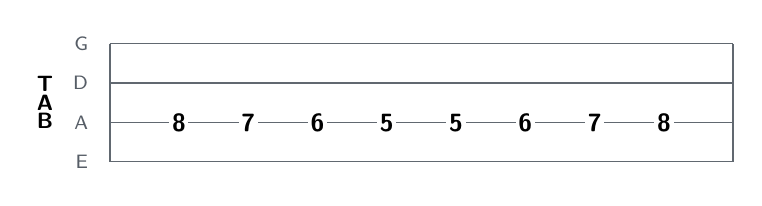
\begin{tikzpicture}[x=1cm,y=0.50cm]
\node[font=\sffamily\bfseries\footnotesize,align=center] at (-0.82,1.50) {T\\[-1mm]A\\[-1mm]B};
\foreach \y/\s in {3/G,2/D,1/A,0/E} {\draw[Ink!70,line width=0.55pt] (0,\y) -- (7.920,\y); \node[anchor=east,font=\sffamily\scriptsize,text=Ink!75] at (-0.15,\y) {\s};}
\draw[Ink!70,line width=0.7pt] (0,0) -- (0,3);
\draw[Ink!70,line width=0.7pt] (7.920,0) -- (7.920,3);
\node[fill=white,inner sep=1.0pt,font=\sffamily\bfseries\small] at (0.880,1) {8};
\node[fill=white,inner sep=1.0pt,font=\sffamily\bfseries\small] at (1.760,1) {7};
\node[fill=white,inner sep=1.0pt,font=\sffamily\bfseries\small] at (2.640,1) {6};
\node[fill=white,inner sep=1.0pt,font=\sffamily\bfseries\small] at (3.520,1) {5};
\node[fill=white,inner sep=1.0pt,font=\sffamily\bfseries\small] at (4.400,1) {5};
\node[fill=white,inner sep=1.0pt,font=\sffamily\bfseries\small] at (5.280,1) {6};
\node[fill=white,inner sep=1.0pt,font=\sffamily\bfseries\small] at (6.160,1) {7};
\node[fill=white,inner sep=1.0pt,font=\sffamily\bfseries\small] at (7.040,1) {8};
\end{tikzpicture}
\endgroup
\end{center}
\begin{tabularx}{\textwidth}{>{\bfseries\sffamily}p{3.0cm}Y}
Target & The fourth finger initiates cleanly without collapsing the hand. \\
Progression & Begin at the lower tempo. Add 4 bpm after three clean repetitions; reduce by 6--8 bpm when timing or muting breaks down. \\
\end{tabularx}
\clearpage
\subsection{P3 - Permutation 1-3-2-4}\label{ex:p3}
\begin{keybox}
\textbf{Five-minute block.} Quarter note = 45--90 bpm; eighth notes.\\
\textbf{Play:} Use fingering 1--3--2--4, then 4--2--3--1. Move the pattern to each string.
\end{keybox}
\begin{center}
{\sffamily\bfseries\small Fretboard}\par\vspace{1mm}
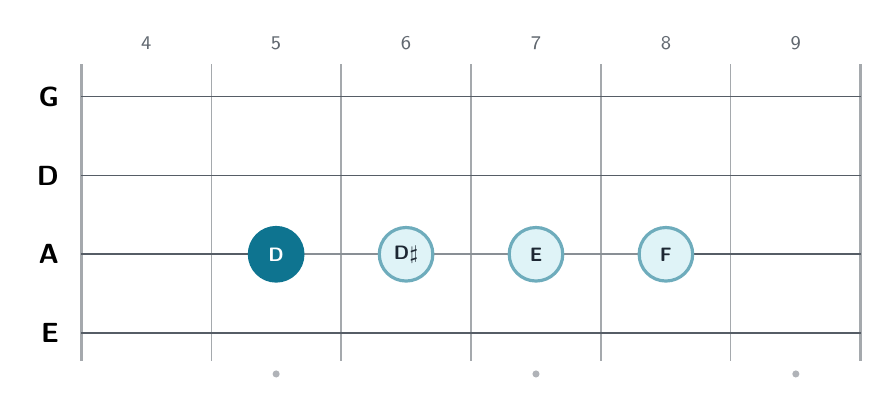
\begin{tikzpicture}[x=1cm,y=1cm,>=stealth]
\node[font=\sffamily\scriptsize,text=Ink!70] at (0.825,4.18) {4};
\node[font=\sffamily\scriptsize,text=Ink!70] at (2.475,4.18) {5};
\node[font=\sffamily\scriptsize,text=Ink!70] at (4.125,4.18) {6};
\node[font=\sffamily\scriptsize,text=Ink!70] at (5.775,4.18) {7};
\node[font=\sffamily\scriptsize,text=Ink!70] at (7.425,4.18) {8};
\node[font=\sffamily\scriptsize,text=Ink!70] at (9.075,4.18) {9};
\draw[Ink!40,line width=1.0pt] (0.000,0.15) -- (0.000,3.92);
\draw[Ink!40,line width=0.45pt] (1.650,0.15) -- (1.650,3.92);
\draw[Ink!40,line width=0.45pt] (3.300,0.15) -- (3.300,3.92);
\draw[Ink!40,line width=0.45pt] (4.950,0.15) -- (4.950,3.92);
\draw[Ink!40,line width=0.45pt] (6.600,0.15) -- (6.600,3.92);
\draw[Ink!40,line width=0.45pt] (8.250,0.15) -- (8.250,3.92);
\draw[Ink!40,line width=1.0pt] (9.900,0.15) -- (9.900,3.92);
\node[anchor=east,font=\sffamily\bfseries] at (-0.16,3.50) {G};
\draw[Ink!75,line width=0.45pt] (0,3.50) -- (9.900,3.50);
\node[anchor=east,font=\sffamily\bfseries] at (-0.16,2.50) {D};
\draw[Ink!75,line width=0.6pt] (0,2.50) -- (9.900,2.50);
\node[anchor=east,font=\sffamily\bfseries] at (-0.16,1.50) {A};
\draw[Ink!75,line width=0.8pt] (0,1.50) -- (9.900,1.50);
\node[anchor=east,font=\sffamily\bfseries] at (-0.16,0.50) {E};
\draw[Ink!75,line width=1.0pt] (0,0.50) -- (9.900,0.50);
\fill[Ink!35] (2.475,-0.02) circle (0.045);
\fill[Ink!35] (5.775,-0.02) circle (0.045);
\fill[Ink!35] (9.075,-0.02) circle (0.045);
\draw[->,Ink!52,line width=0.65pt] (2.475,1.500) -- (5.775,1.500);
\draw[->,Ink!52,line width=0.65pt] (5.775,1.500) -- (4.125,1.500);
\draw[->,Ink!52,line width=0.65pt] (4.125,1.500) -- (7.425,1.500);
\node[circle,minimum size=0.68cm,inner sep=0pt,fill=Accent,draw=Accent,text=white,line width=1.15pt,font=\sffamily\bfseries\scriptsize] at (2.475,1.500) {D};
\node[circle,minimum size=0.68cm,inner sep=0pt,fill=AccentLight,draw=Accent!60,text=Ink,line width=1.15pt,font=\sffamily\bfseries\scriptsize] at (5.775,1.500) {E};
\node[circle,minimum size=0.68cm,inner sep=0pt,fill=AccentLight,draw=Accent!60,text=Ink,line width=1.15pt,font=\sffamily\bfseries\scriptsize] at (4.125,1.500) {D$\sharp$};
\node[circle,minimum size=0.68cm,inner sep=0pt,fill=AccentLight,draw=Accent!60,text=Ink,line width=1.15pt,font=\sffamily\bfseries\scriptsize] at (7.425,1.500) {F};
\end{tikzpicture}
\end{center}
\begin{center}
\begingroup
\setlength{\parindent}{0pt}
\begin{minipage}{0.88\textwidth}
{\sffamily\bfseries\small Standard notation}\par\vspace{-1mm}
\begin{music}
\instrumentnumber{1}
\setstaffs1{1}
\setclef1{\bass}
\generalmeter{\meterfrac44}
\nobarnumbers
\nostartrule
\startextract
\Notes\cu{K}\cu{L}\cu{^K}\cu{M}\cu{M}\cu{K}\cu{L}\cu{=K}\en
\zendextract
\end{music}
\end{minipage}
\endgroup
\end{center}
\begin{center}
\begingroup
{\sffamily\bfseries\small Bass TAB}\par\vspace{1mm}
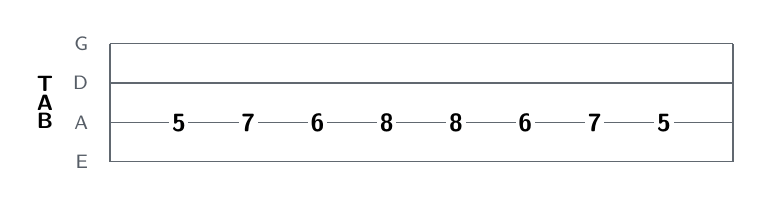
\begin{tikzpicture}[x=1cm,y=0.50cm]
\node[font=\sffamily\bfseries\footnotesize,align=center] at (-0.82,1.50) {T\\[-1mm]A\\[-1mm]B};
\foreach \y/\s in {3/G,2/D,1/A,0/E} {\draw[Ink!70,line width=0.55pt] (0,\y) -- (7.920,\y); \node[anchor=east,font=\sffamily\scriptsize,text=Ink!75] at (-0.15,\y) {\s};}
\draw[Ink!70,line width=0.7pt] (0,0) -- (0,3);
\draw[Ink!70,line width=0.7pt] (7.920,0) -- (7.920,3);
\node[fill=white,inner sep=1.0pt,font=\sffamily\bfseries\small] at (0.880,1) {5};
\node[fill=white,inner sep=1.0pt,font=\sffamily\bfseries\small] at (1.760,1) {7};
\node[fill=white,inner sep=1.0pt,font=\sffamily\bfseries\small] at (2.640,1) {6};
\node[fill=white,inner sep=1.0pt,font=\sffamily\bfseries\small] at (3.520,1) {8};
\node[fill=white,inner sep=1.0pt,font=\sffamily\bfseries\small] at (4.400,1) {8};
\node[fill=white,inner sep=1.0pt,font=\sffamily\bfseries\small] at (5.280,1) {6};
\node[fill=white,inner sep=1.0pt,font=\sffamily\bfseries\small] at (6.160,1) {7};
\node[fill=white,inner sep=1.0pt,font=\sffamily\bfseries\small] at (7.040,1) {5};
\end{tikzpicture}
\endgroup
\end{center}
\begin{tabularx}{\textwidth}{>{\bfseries\sffamily}p{3.0cm}Y}
Target & No finger moves before its note is required. \\
Progression & Begin at the lower tempo. Add 4 bpm after three clean repetitions; reduce by 6--8 bpm when timing or muting breaks down. \\
\end{tabularx}
\clearpage
\subsection{P4 - Permutation 1-4-2-3}\label{ex:p4}
\begin{keybox}
\textbf{Five-minute block.} Quarter note = 40--85 bpm; eighth notes.\\
\textbf{Play:} Use fingering 1--4--2--3 and reverse. Keep the thumb relaxed behind the neck.
\end{keybox}
\begin{center}
{\sffamily\bfseries\small Fretboard}\par\vspace{1mm}
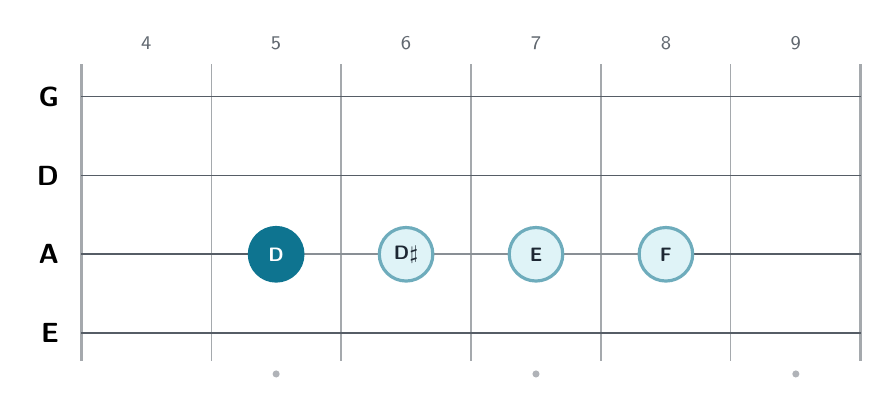
\begin{tikzpicture}[x=1cm,y=1cm,>=stealth]
\node[font=\sffamily\scriptsize,text=Ink!70] at (0.825,4.18) {4};
\node[font=\sffamily\scriptsize,text=Ink!70] at (2.475,4.18) {5};
\node[font=\sffamily\scriptsize,text=Ink!70] at (4.125,4.18) {6};
\node[font=\sffamily\scriptsize,text=Ink!70] at (5.775,4.18) {7};
\node[font=\sffamily\scriptsize,text=Ink!70] at (7.425,4.18) {8};
\node[font=\sffamily\scriptsize,text=Ink!70] at (9.075,4.18) {9};
\draw[Ink!40,line width=1.0pt] (0.000,0.15) -- (0.000,3.92);
\draw[Ink!40,line width=0.45pt] (1.650,0.15) -- (1.650,3.92);
\draw[Ink!40,line width=0.45pt] (3.300,0.15) -- (3.300,3.92);
\draw[Ink!40,line width=0.45pt] (4.950,0.15) -- (4.950,3.92);
\draw[Ink!40,line width=0.45pt] (6.600,0.15) -- (6.600,3.92);
\draw[Ink!40,line width=0.45pt] (8.250,0.15) -- (8.250,3.92);
\draw[Ink!40,line width=1.0pt] (9.900,0.15) -- (9.900,3.92);
\node[anchor=east,font=\sffamily\bfseries] at (-0.16,3.50) {G};
\draw[Ink!75,line width=0.45pt] (0,3.50) -- (9.900,3.50);
\node[anchor=east,font=\sffamily\bfseries] at (-0.16,2.50) {D};
\draw[Ink!75,line width=0.6pt] (0,2.50) -- (9.900,2.50);
\node[anchor=east,font=\sffamily\bfseries] at (-0.16,1.50) {A};
\draw[Ink!75,line width=0.8pt] (0,1.50) -- (9.900,1.50);
\node[anchor=east,font=\sffamily\bfseries] at (-0.16,0.50) {E};
\draw[Ink!75,line width=1.0pt] (0,0.50) -- (9.900,0.50);
\fill[Ink!35] (2.475,-0.02) circle (0.045);
\fill[Ink!35] (5.775,-0.02) circle (0.045);
\fill[Ink!35] (9.075,-0.02) circle (0.045);
\draw[->,Ink!52,line width=0.65pt] (2.475,1.500) -- (7.425,1.500);
\draw[->,Ink!52,line width=0.65pt] (7.425,1.500) -- (4.125,1.500);
\draw[->,Ink!52,line width=0.65pt] (4.125,1.500) -- (5.775,1.500);
\node[circle,minimum size=0.68cm,inner sep=0pt,fill=Accent,draw=Accent,text=white,line width=1.15pt,font=\sffamily\bfseries\scriptsize] at (2.475,1.500) {D};
\node[circle,minimum size=0.68cm,inner sep=0pt,fill=AccentLight,draw=Accent!60,text=Ink,line width=1.15pt,font=\sffamily\bfseries\scriptsize] at (7.425,1.500) {F};
\node[circle,minimum size=0.68cm,inner sep=0pt,fill=AccentLight,draw=Accent!60,text=Ink,line width=1.15pt,font=\sffamily\bfseries\scriptsize] at (4.125,1.500) {D$\sharp$};
\node[circle,minimum size=0.68cm,inner sep=0pt,fill=AccentLight,draw=Accent!60,text=Ink,line width=1.15pt,font=\sffamily\bfseries\scriptsize] at (5.775,1.500) {E};
\end{tikzpicture}
\end{center}
\begin{center}
\begingroup
\setlength{\parindent}{0pt}
\begin{minipage}{0.88\textwidth}
{\sffamily\bfseries\small Standard notation}\par\vspace{-1mm}
\begin{music}
\instrumentnumber{1}
\setstaffs1{1}
\setclef1{\bass}
\generalmeter{\meterfrac44}
\nobarnumbers
\nostartrule
\startextract
\Notes\cu{K}\cu{M}\cu{^K}\cu{L}\cu{L}\cu{K}\cu{M}\cu{=K}\en
\zendextract
\end{music}
\end{minipage}
\endgroup
\end{center}
\begin{center}
\begingroup
{\sffamily\bfseries\small Bass TAB}\par\vspace{1mm}
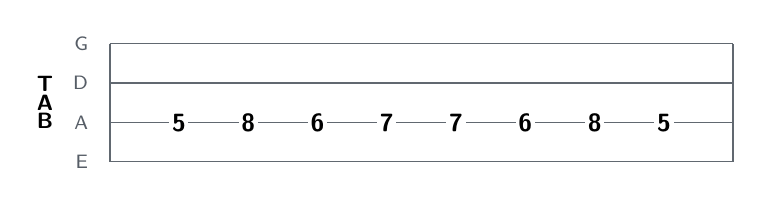
\begin{tikzpicture}[x=1cm,y=0.50cm]
\node[font=\sffamily\bfseries\footnotesize,align=center] at (-0.82,1.50) {T\\[-1mm]A\\[-1mm]B};
\foreach \y/\s in {3/G,2/D,1/A,0/E} {\draw[Ink!70,line width=0.55pt] (0,\y) -- (7.920,\y); \node[anchor=east,font=\sffamily\scriptsize,text=Ink!75] at (-0.15,\y) {\s};}
\draw[Ink!70,line width=0.7pt] (0,0) -- (0,3);
\draw[Ink!70,line width=0.7pt] (7.920,0) -- (7.920,3);
\node[fill=white,inner sep=1.0pt,font=\sffamily\bfseries\small] at (0.880,1) {5};
\node[fill=white,inner sep=1.0pt,font=\sffamily\bfseries\small] at (1.760,1) {8};
\node[fill=white,inner sep=1.0pt,font=\sffamily\bfseries\small] at (2.640,1) {6};
\node[fill=white,inner sep=1.0pt,font=\sffamily\bfseries\small] at (3.520,1) {7};
\node[fill=white,inner sep=1.0pt,font=\sffamily\bfseries\small] at (4.400,1) {7};
\node[fill=white,inner sep=1.0pt,font=\sffamily\bfseries\small] at (5.280,1) {6};
\node[fill=white,inner sep=1.0pt,font=\sffamily\bfseries\small] at (6.160,1) {8};
\node[fill=white,inner sep=1.0pt,font=\sffamily\bfseries\small] at (7.040,1) {5};
\end{tikzpicture}
\endgroup
\end{center}
\begin{tabularx}{\textwidth}{>{\bfseries\sffamily}p{3.0cm}Y}
Target & The 1-to-4 reach stays quiet and controlled. \\
Progression & Begin at the lower tempo. Add 4 bpm after three clean repetitions; reduce by 6--8 bpm when timing or muting breaks down. \\
\end{tabularx}
\clearpage
\subsection{P5 - Same-fret string ladder}\label{ex:p5}
\begin{keybox}
\textbf{Five-minute block.} Quarter note = 50--110 bpm; eighth notes.\\
\textbf{Play:} Cross all four strings at fret 5 and return. Alternate plucking fingers continuously.
\end{keybox}
\begin{center}
{\sffamily\bfseries\small Fretboard}\par\vspace{1mm}
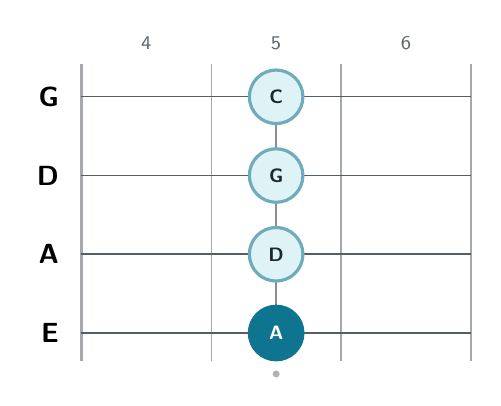
\begin{tikzpicture}[x=1cm,y=1cm,>=stealth]
\node[font=\sffamily\scriptsize,text=Ink!70] at (0.825,4.18) {4};
\node[font=\sffamily\scriptsize,text=Ink!70] at (2.475,4.18) {5};
\node[font=\sffamily\scriptsize,text=Ink!70] at (4.125,4.18) {6};
\draw[Ink!40,line width=1.0pt] (0.000,0.15) -- (0.000,3.92);
\draw[Ink!40,line width=0.45pt] (1.650,0.15) -- (1.650,3.92);
\draw[Ink!40,line width=0.45pt] (3.300,0.15) -- (3.300,3.92);
\draw[Ink!40,line width=1.0pt] (4.950,0.15) -- (4.950,3.92);
\node[anchor=east,font=\sffamily\bfseries] at (-0.16,3.50) {G};
\draw[Ink!75,line width=0.45pt] (0,3.50) -- (4.950,3.50);
\node[anchor=east,font=\sffamily\bfseries] at (-0.16,2.50) {D};
\draw[Ink!75,line width=0.6pt] (0,2.50) -- (4.950,2.50);
\node[anchor=east,font=\sffamily\bfseries] at (-0.16,1.50) {A};
\draw[Ink!75,line width=0.8pt] (0,1.50) -- (4.950,1.50);
\node[anchor=east,font=\sffamily\bfseries] at (-0.16,0.50) {E};
\draw[Ink!75,line width=1.0pt] (0,0.50) -- (4.950,0.50);
\fill[Ink!35] (2.475,-0.02) circle (0.045);
\draw[->,Ink!52,line width=0.65pt] (2.475,0.500) -- (2.475,1.500);
\draw[->,Ink!52,line width=0.65pt] (2.475,1.500) -- (2.475,2.500);
\draw[->,Ink!52,line width=0.65pt] (2.475,2.500) -- (2.475,3.500);
\node[circle,minimum size=0.68cm,inner sep=0pt,fill=Accent,draw=Accent,text=white,line width=1.15pt,font=\sffamily\bfseries\scriptsize] at (2.475,0.500) {A};
\node[circle,minimum size=0.68cm,inner sep=0pt,fill=AccentLight,draw=Accent!60,text=Ink,line width=1.15pt,font=\sffamily\bfseries\scriptsize] at (2.475,1.500) {D};
\node[circle,minimum size=0.68cm,inner sep=0pt,fill=AccentLight,draw=Accent!60,text=Ink,line width=1.15pt,font=\sffamily\bfseries\scriptsize] at (2.475,2.500) {G};
\node[circle,minimum size=0.68cm,inner sep=0pt,fill=AccentLight,draw=Accent!60,text=Ink,line width=1.15pt,font=\sffamily\bfseries\scriptsize] at (2.475,3.500) {C};
\end{tikzpicture}
\end{center}
\begin{center}
\begingroup
\setlength{\parindent}{0pt}
\begin{minipage}{0.88\textwidth}
{\sffamily\bfseries\small Standard notation}\par\vspace{-1mm}
\begin{music}
\instrumentnumber{1}
\setstaffs1{1}
\setclef1{\bass}
\generalmeter{\meterfrac44}
\nobarnumbers
\nostartrule
\startextract
\Notes\cu{H}\cu{K}\cu{N}\cu{c}\cu{c}\cu{N}\cu{K}\cu{H}\en
\zendextract
\end{music}
\end{minipage}
\endgroup
\end{center}
\begin{center}
\begingroup
{\sffamily\bfseries\small Bass TAB}\par\vspace{1mm}
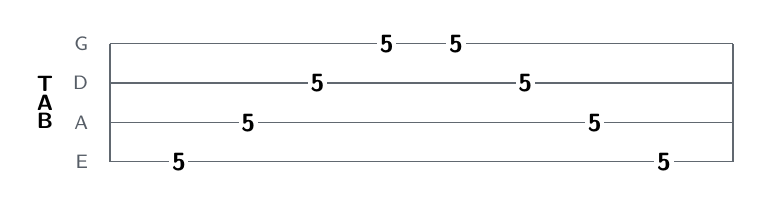
\begin{tikzpicture}[x=1cm,y=0.50cm]
\node[font=\sffamily\bfseries\footnotesize,align=center] at (-0.82,1.50) {T\\[-1mm]A\\[-1mm]B};
\foreach \y/\s in {3/G,2/D,1/A,0/E} {\draw[Ink!70,line width=0.55pt] (0,\y) -- (7.920,\y); \node[anchor=east,font=\sffamily\scriptsize,text=Ink!75] at (-0.15,\y) {\s};}
\draw[Ink!70,line width=0.7pt] (0,0) -- (0,3);
\draw[Ink!70,line width=0.7pt] (7.920,0) -- (7.920,3);
\node[fill=white,inner sep=1.0pt,font=\sffamily\bfseries\small] at (0.880,0) {5};
\node[fill=white,inner sep=1.0pt,font=\sffamily\bfseries\small] at (1.760,1) {5};
\node[fill=white,inner sep=1.0pt,font=\sffamily\bfseries\small] at (2.640,2) {5};
\node[fill=white,inner sep=1.0pt,font=\sffamily\bfseries\small] at (3.520,3) {5};
\node[fill=white,inner sep=1.0pt,font=\sffamily\bfseries\small] at (4.400,3) {5};
\node[fill=white,inner sep=1.0pt,font=\sffamily\bfseries\small] at (5.280,2) {5};
\node[fill=white,inner sep=1.0pt,font=\sffamily\bfseries\small] at (6.160,1) {5};
\node[fill=white,inner sep=1.0pt,font=\sffamily\bfseries\small] at (7.040,0) {5};
\end{tikzpicture}
\endgroup
\end{center}
\begin{tabularx}{\textwidth}{>{\bfseries\sffamily}p{3.0cm}Y}
Target & No open-string ringing during either direction change. \\
Progression & Begin at the lower tempo. Add 4 bpm after three clean repetitions; reduce by 6--8 bpm when timing or muting breaks down. \\
\end{tabularx}
\clearpage
\subsection{P6 - Diagonal spider outward}\label{ex:p6}
\begin{keybox}
\textbf{Five-minute block.} Quarter note = 40--80 bpm; eighth notes.\\
\textbf{Play:} Assign fingers 1--2--3--4 to the first diagonal, then 1--2--3--4 to the returning diagonal.
\end{keybox}
\begin{center}
{\sffamily\bfseries\small Fretboard}\par\vspace{1mm}
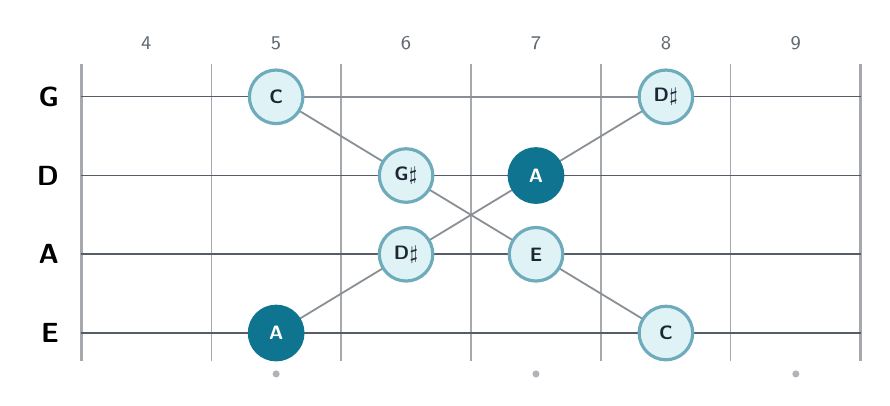
\begin{tikzpicture}[x=1cm,y=1cm,>=stealth]
\node[font=\sffamily\scriptsize,text=Ink!70] at (0.825,4.18) {4};
\node[font=\sffamily\scriptsize,text=Ink!70] at (2.475,4.18) {5};
\node[font=\sffamily\scriptsize,text=Ink!70] at (4.125,4.18) {6};
\node[font=\sffamily\scriptsize,text=Ink!70] at (5.775,4.18) {7};
\node[font=\sffamily\scriptsize,text=Ink!70] at (7.425,4.18) {8};
\node[font=\sffamily\scriptsize,text=Ink!70] at (9.075,4.18) {9};
\draw[Ink!40,line width=1.0pt] (0.000,0.15) -- (0.000,3.92);
\draw[Ink!40,line width=0.45pt] (1.650,0.15) -- (1.650,3.92);
\draw[Ink!40,line width=0.45pt] (3.300,0.15) -- (3.300,3.92);
\draw[Ink!40,line width=0.45pt] (4.950,0.15) -- (4.950,3.92);
\draw[Ink!40,line width=0.45pt] (6.600,0.15) -- (6.600,3.92);
\draw[Ink!40,line width=0.45pt] (8.250,0.15) -- (8.250,3.92);
\draw[Ink!40,line width=1.0pt] (9.900,0.15) -- (9.900,3.92);
\node[anchor=east,font=\sffamily\bfseries] at (-0.16,3.50) {G};
\draw[Ink!75,line width=0.45pt] (0,3.50) -- (9.900,3.50);
\node[anchor=east,font=\sffamily\bfseries] at (-0.16,2.50) {D};
\draw[Ink!75,line width=0.6pt] (0,2.50) -- (9.900,2.50);
\node[anchor=east,font=\sffamily\bfseries] at (-0.16,1.50) {A};
\draw[Ink!75,line width=0.8pt] (0,1.50) -- (9.900,1.50);
\node[anchor=east,font=\sffamily\bfseries] at (-0.16,0.50) {E};
\draw[Ink!75,line width=1.0pt] (0,0.50) -- (9.900,0.50);
\fill[Ink!35] (2.475,-0.02) circle (0.045);
\fill[Ink!35] (5.775,-0.02) circle (0.045);
\fill[Ink!35] (9.075,-0.02) circle (0.045);
\draw[->,Ink!52,line width=0.65pt] (2.475,0.500) -- (4.125,1.500);
\draw[->,Ink!52,line width=0.65pt] (4.125,1.500) -- (5.775,2.500);
\draw[->,Ink!52,line width=0.65pt] (5.775,2.500) -- (7.425,3.500);
\draw[->,Ink!52,line width=0.65pt] (7.425,3.500) -- (2.475,3.500);
\draw[->,Ink!52,line width=0.65pt] (2.475,3.500) -- (4.125,2.500);
\draw[->,Ink!52,line width=0.65pt] (4.125,2.500) -- (5.775,1.500);
\draw[->,Ink!52,line width=0.65pt] (5.775,1.500) -- (7.425,0.500);
\node[circle,minimum size=0.68cm,inner sep=0pt,fill=Accent,draw=Accent,text=white,line width=1.15pt,font=\sffamily\bfseries\scriptsize] at (2.475,0.500) {A};
\node[circle,minimum size=0.68cm,inner sep=0pt,fill=AccentLight,draw=Accent!60,text=Ink,line width=1.15pt,font=\sffamily\bfseries\scriptsize] at (4.125,1.500) {D$\sharp$};
\node[circle,minimum size=0.68cm,inner sep=0pt,fill=Accent,draw=Accent,text=white,line width=1.15pt,font=\sffamily\bfseries\scriptsize] at (5.775,2.500) {A};
\node[circle,minimum size=0.68cm,inner sep=0pt,fill=AccentLight,draw=Accent!60,text=Ink,line width=1.15pt,font=\sffamily\bfseries\scriptsize] at (7.425,3.500) {D$\sharp$};
\node[circle,minimum size=0.68cm,inner sep=0pt,fill=AccentLight,draw=Accent!60,text=Ink,line width=1.15pt,font=\sffamily\bfseries\scriptsize] at (2.475,3.500) {C};
\node[circle,minimum size=0.68cm,inner sep=0pt,fill=AccentLight,draw=Accent!60,text=Ink,line width=1.15pt,font=\sffamily\bfseries\scriptsize] at (4.125,2.500) {G$\sharp$};
\node[circle,minimum size=0.68cm,inner sep=0pt,fill=AccentLight,draw=Accent!60,text=Ink,line width=1.15pt,font=\sffamily\bfseries\scriptsize] at (5.775,1.500) {E};
\node[circle,minimum size=0.68cm,inner sep=0pt,fill=AccentLight,draw=Accent!60,text=Ink,line width=1.15pt,font=\sffamily\bfseries\scriptsize] at (7.425,0.500) {C};
\end{tikzpicture}
\end{center}
\begin{center}
\begingroup
\setlength{\parindent}{0pt}
\begin{minipage}{0.88\textwidth}
{\sffamily\bfseries\small Standard notation}\par\vspace{-1mm}
\begin{music}
\instrumentnumber{1}
\setstaffs1{1}
\setclef1{\bass}
\generalmeter{\meterfrac44}
\nobarnumbers
\nostartrule
\startextract
\Notes\cu{H}\cu{^K}\cu{a}\cu{d}\cu{c}\cu{^N}\cu{L}\cu{J}\en
\zendextract
\end{music}
\end{minipage}
\endgroup
\end{center}
\begin{center}
\begingroup
{\sffamily\bfseries\small Bass TAB}\par\vspace{1mm}
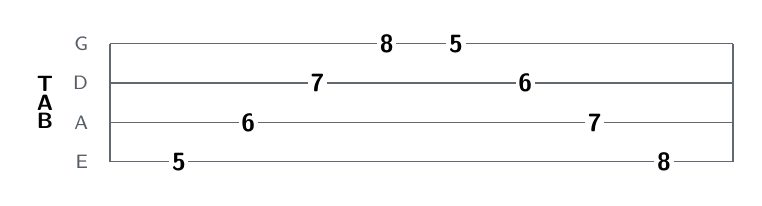
\begin{tikzpicture}[x=1cm,y=0.50cm]
\node[font=\sffamily\bfseries\footnotesize,align=center] at (-0.82,1.50) {T\\[-1mm]A\\[-1mm]B};
\foreach \y/\s in {3/G,2/D,1/A,0/E} {\draw[Ink!70,line width=0.55pt] (0,\y) -- (7.920,\y); \node[anchor=east,font=\sffamily\scriptsize,text=Ink!75] at (-0.15,\y) {\s};}
\draw[Ink!70,line width=0.7pt] (0,0) -- (0,3);
\draw[Ink!70,line width=0.7pt] (7.920,0) -- (7.920,3);
\node[fill=white,inner sep=1.0pt,font=\sffamily\bfseries\small] at (0.880,0) {5};
\node[fill=white,inner sep=1.0pt,font=\sffamily\bfseries\small] at (1.760,1) {6};
\node[fill=white,inner sep=1.0pt,font=\sffamily\bfseries\small] at (2.640,2) {7};
\node[fill=white,inner sep=1.0pt,font=\sffamily\bfseries\small] at (3.520,3) {8};
\node[fill=white,inner sep=1.0pt,font=\sffamily\bfseries\small] at (4.400,3) {5};
\node[fill=white,inner sep=1.0pt,font=\sffamily\bfseries\small] at (5.280,2) {6};
\node[fill=white,inner sep=1.0pt,font=\sffamily\bfseries\small] at (6.160,1) {7};
\node[fill=white,inner sep=1.0pt,font=\sffamily\bfseries\small] at (7.040,0) {8};
\end{tikzpicture}
\endgroup
\end{center}
\begin{tabularx}{\textwidth}{>{\bfseries\sffamily}p{3.0cm}Y}
Target & Every string change is muted before the next note sounds. \\
Progression & Begin at the lower tempo. Add 4 bpm after three clean repetitions; reduce by 6--8 bpm when timing or muting breaks down. \\
\end{tabularx}
\clearpage
\subsection{P7 - Diagonal spider inward}\label{ex:p7}
\begin{keybox}
\textbf{Five-minute block.} Quarter note = 40--80 bpm; eighth notes.\\
\textbf{Play:} Reverse the diagonal direction from P6 while preserving finger assignments.
\end{keybox}
\begin{center}
{\sffamily\bfseries\small Fretboard}\par\vspace{1mm}
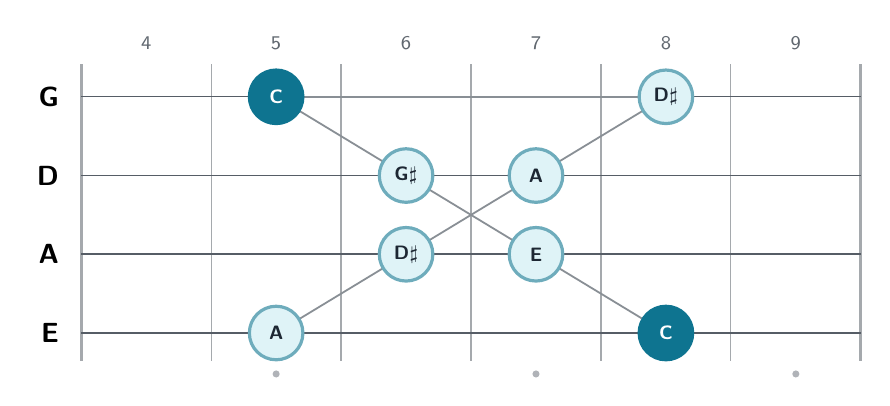
\begin{tikzpicture}[x=1cm,y=1cm,>=stealth]
\node[font=\sffamily\scriptsize,text=Ink!70] at (0.825,4.18) {4};
\node[font=\sffamily\scriptsize,text=Ink!70] at (2.475,4.18) {5};
\node[font=\sffamily\scriptsize,text=Ink!70] at (4.125,4.18) {6};
\node[font=\sffamily\scriptsize,text=Ink!70] at (5.775,4.18) {7};
\node[font=\sffamily\scriptsize,text=Ink!70] at (7.425,4.18) {8};
\node[font=\sffamily\scriptsize,text=Ink!70] at (9.075,4.18) {9};
\draw[Ink!40,line width=1.0pt] (0.000,0.15) -- (0.000,3.92);
\draw[Ink!40,line width=0.45pt] (1.650,0.15) -- (1.650,3.92);
\draw[Ink!40,line width=0.45pt] (3.300,0.15) -- (3.300,3.92);
\draw[Ink!40,line width=0.45pt] (4.950,0.15) -- (4.950,3.92);
\draw[Ink!40,line width=0.45pt] (6.600,0.15) -- (6.600,3.92);
\draw[Ink!40,line width=0.45pt] (8.250,0.15) -- (8.250,3.92);
\draw[Ink!40,line width=1.0pt] (9.900,0.15) -- (9.900,3.92);
\node[anchor=east,font=\sffamily\bfseries] at (-0.16,3.50) {G};
\draw[Ink!75,line width=0.45pt] (0,3.50) -- (9.900,3.50);
\node[anchor=east,font=\sffamily\bfseries] at (-0.16,2.50) {D};
\draw[Ink!75,line width=0.6pt] (0,2.50) -- (9.900,2.50);
\node[anchor=east,font=\sffamily\bfseries] at (-0.16,1.50) {A};
\draw[Ink!75,line width=0.8pt] (0,1.50) -- (9.900,1.50);
\node[anchor=east,font=\sffamily\bfseries] at (-0.16,0.50) {E};
\draw[Ink!75,line width=1.0pt] (0,0.50) -- (9.900,0.50);
\fill[Ink!35] (2.475,-0.02) circle (0.045);
\fill[Ink!35] (5.775,-0.02) circle (0.045);
\fill[Ink!35] (9.075,-0.02) circle (0.045);
\draw[->,Ink!52,line width=0.65pt] (7.425,0.500) -- (5.775,1.500);
\draw[->,Ink!52,line width=0.65pt] (5.775,1.500) -- (4.125,2.500);
\draw[->,Ink!52,line width=0.65pt] (4.125,2.500) -- (2.475,3.500);
\draw[->,Ink!52,line width=0.65pt] (2.475,3.500) -- (7.425,3.500);
\draw[->,Ink!52,line width=0.65pt] (7.425,3.500) -- (5.775,2.500);
\draw[->,Ink!52,line width=0.65pt] (5.775,2.500) -- (4.125,1.500);
\draw[->,Ink!52,line width=0.65pt] (4.125,1.500) -- (2.475,0.500);
\node[circle,minimum size=0.68cm,inner sep=0pt,fill=Accent,draw=Accent,text=white,line width=1.15pt,font=\sffamily\bfseries\scriptsize] at (7.425,0.500) {C};
\node[circle,minimum size=0.68cm,inner sep=0pt,fill=AccentLight,draw=Accent!60,text=Ink,line width=1.15pt,font=\sffamily\bfseries\scriptsize] at (5.775,1.500) {E};
\node[circle,minimum size=0.68cm,inner sep=0pt,fill=AccentLight,draw=Accent!60,text=Ink,line width=1.15pt,font=\sffamily\bfseries\scriptsize] at (4.125,2.500) {G$\sharp$};
\node[circle,minimum size=0.68cm,inner sep=0pt,fill=Accent,draw=Accent,text=white,line width=1.15pt,font=\sffamily\bfseries\scriptsize] at (2.475,3.500) {C};
\node[circle,minimum size=0.68cm,inner sep=0pt,fill=AccentLight,draw=Accent!60,text=Ink,line width=1.15pt,font=\sffamily\bfseries\scriptsize] at (7.425,3.500) {D$\sharp$};
\node[circle,minimum size=0.68cm,inner sep=0pt,fill=AccentLight,draw=Accent!60,text=Ink,line width=1.15pt,font=\sffamily\bfseries\scriptsize] at (5.775,2.500) {A};
\node[circle,minimum size=0.68cm,inner sep=0pt,fill=AccentLight,draw=Accent!60,text=Ink,line width=1.15pt,font=\sffamily\bfseries\scriptsize] at (4.125,1.500) {D$\sharp$};
\node[circle,minimum size=0.68cm,inner sep=0pt,fill=AccentLight,draw=Accent!60,text=Ink,line width=1.15pt,font=\sffamily\bfseries\scriptsize] at (2.475,0.500) {A};
\end{tikzpicture}
\end{center}
\begin{center}
\begingroup
\setlength{\parindent}{0pt}
\begin{minipage}{0.88\textwidth}
{\sffamily\bfseries\small Standard notation}\par\vspace{-1mm}
\begin{music}
\instrumentnumber{1}
\setstaffs1{1}
\setclef1{\bass}
\generalmeter{\meterfrac44}
\nobarnumbers
\nostartrule
\startextract
\Notes\cu{J}\cu{L}\cu{^N}\cu{c}\cu{^d}\cu{a}\cu{K}\cu{H}\en
\zendextract
\end{music}
\end{minipage}
\endgroup
\end{center}
\begin{center}
\begingroup
{\sffamily\bfseries\small Bass TAB}\par\vspace{1mm}
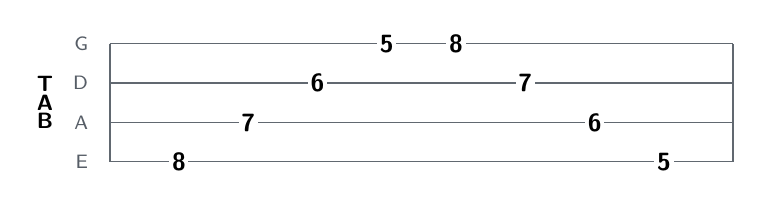
\begin{tikzpicture}[x=1cm,y=0.50cm]
\node[font=\sffamily\bfseries\footnotesize,align=center] at (-0.82,1.50) {T\\[-1mm]A\\[-1mm]B};
\foreach \y/\s in {3/G,2/D,1/A,0/E} {\draw[Ink!70,line width=0.55pt] (0,\y) -- (7.920,\y); \node[anchor=east,font=\sffamily\scriptsize,text=Ink!75] at (-0.15,\y) {\s};}
\draw[Ink!70,line width=0.7pt] (0,0) -- (0,3);
\draw[Ink!70,line width=0.7pt] (7.920,0) -- (7.920,3);
\node[fill=white,inner sep=1.0pt,font=\sffamily\bfseries\small] at (0.880,0) {8};
\node[fill=white,inner sep=1.0pt,font=\sffamily\bfseries\small] at (1.760,1) {7};
\node[fill=white,inner sep=1.0pt,font=\sffamily\bfseries\small] at (2.640,2) {6};
\node[fill=white,inner sep=1.0pt,font=\sffamily\bfseries\small] at (3.520,3) {5};
\node[fill=white,inner sep=1.0pt,font=\sffamily\bfseries\small] at (4.400,3) {8};
\node[fill=white,inner sep=1.0pt,font=\sffamily\bfseries\small] at (5.280,2) {7};
\node[fill=white,inner sep=1.0pt,font=\sffamily\bfseries\small] at (6.160,1) {6};
\node[fill=white,inner sep=1.0pt,font=\sffamily\bfseries\small] at (7.040,0) {5};
\end{tikzpicture}
\endgroup
\end{center}
\begin{tabularx}{\textwidth}{>{\bfseries\sffamily}p{3.0cm}Y}
Target & The hand remains centered; the wrist does not twist between strings. \\
Progression & Begin at the lower tempo. Add 4 bpm after three clean repetitions; reduce by 6--8 bpm when timing or muting breaks down. \\
\end{tabularx}
\clearpage
\subsection{P8 - String-skipping ladder}\label{ex:p8}
\begin{keybox}
\textbf{Five-minute block.} Quarter note = 45--95 bpm; eighth notes.\\
\textbf{Play:} Skip one string on every move. Use movable-thumb or floating-thumb muting.
\end{keybox}
\begin{center}
{\sffamily\bfseries\small Fretboard}\par\vspace{1mm}
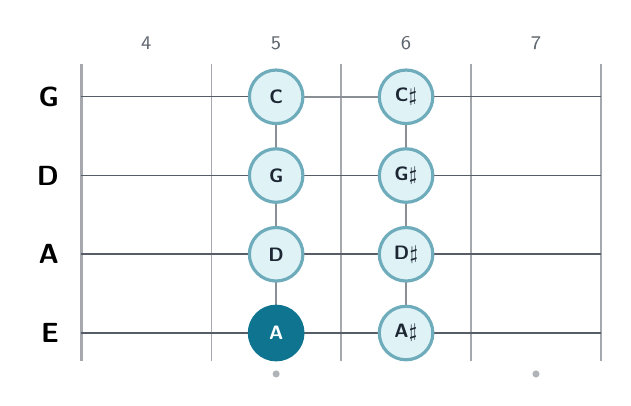
\begin{tikzpicture}[x=1cm,y=1cm,>=stealth]
\node[font=\sffamily\scriptsize,text=Ink!70] at (0.825,4.18) {4};
\node[font=\sffamily\scriptsize,text=Ink!70] at (2.475,4.18) {5};
\node[font=\sffamily\scriptsize,text=Ink!70] at (4.125,4.18) {6};
\node[font=\sffamily\scriptsize,text=Ink!70] at (5.775,4.18) {7};
\draw[Ink!40,line width=1.0pt] (0.000,0.15) -- (0.000,3.92);
\draw[Ink!40,line width=0.45pt] (1.650,0.15) -- (1.650,3.92);
\draw[Ink!40,line width=0.45pt] (3.300,0.15) -- (3.300,3.92);
\draw[Ink!40,line width=0.45pt] (4.950,0.15) -- (4.950,3.92);
\draw[Ink!40,line width=1.0pt] (6.600,0.15) -- (6.600,3.92);
\node[anchor=east,font=\sffamily\bfseries] at (-0.16,3.50) {G};
\draw[Ink!75,line width=0.45pt] (0,3.50) -- (6.600,3.50);
\node[anchor=east,font=\sffamily\bfseries] at (-0.16,2.50) {D};
\draw[Ink!75,line width=0.6pt] (0,2.50) -- (6.600,2.50);
\node[anchor=east,font=\sffamily\bfseries] at (-0.16,1.50) {A};
\draw[Ink!75,line width=0.8pt] (0,1.50) -- (6.600,1.50);
\node[anchor=east,font=\sffamily\bfseries] at (-0.16,0.50) {E};
\draw[Ink!75,line width=1.0pt] (0,0.50) -- (6.600,0.50);
\fill[Ink!35] (2.475,-0.02) circle (0.045);
\fill[Ink!35] (5.775,-0.02) circle (0.045);
\draw[->,Ink!52,line width=0.65pt] (2.475,0.500) -- (2.475,2.500);
\draw[->,Ink!52,line width=0.65pt] (2.475,2.500) -- (2.475,1.500);
\draw[->,Ink!52,line width=0.65pt] (2.475,1.500) -- (2.475,3.500);
\draw[->,Ink!52,line width=0.65pt] (2.475,3.500) -- (4.125,3.500);
\draw[->,Ink!52,line width=0.65pt] (4.125,3.500) -- (4.125,1.500);
\draw[->,Ink!52,line width=0.65pt] (4.125,1.500) -- (4.125,2.500);
\draw[->,Ink!52,line width=0.65pt] (4.125,2.500) -- (4.125,0.500);
\node[circle,minimum size=0.68cm,inner sep=0pt,fill=Accent,draw=Accent,text=white,line width=1.15pt,font=\sffamily\bfseries\scriptsize] at (2.475,0.500) {A};
\node[circle,minimum size=0.68cm,inner sep=0pt,fill=AccentLight,draw=Accent!60,text=Ink,line width=1.15pt,font=\sffamily\bfseries\scriptsize] at (2.475,2.500) {G};
\node[circle,minimum size=0.68cm,inner sep=0pt,fill=AccentLight,draw=Accent!60,text=Ink,line width=1.15pt,font=\sffamily\bfseries\scriptsize] at (2.475,1.500) {D};
\node[circle,minimum size=0.68cm,inner sep=0pt,fill=AccentLight,draw=Accent!60,text=Ink,line width=1.15pt,font=\sffamily\bfseries\scriptsize] at (2.475,3.500) {C};
\node[circle,minimum size=0.68cm,inner sep=0pt,fill=AccentLight,draw=Accent!60,text=Ink,line width=1.15pt,font=\sffamily\bfseries\scriptsize] at (4.125,3.500) {C$\sharp$};
\node[circle,minimum size=0.68cm,inner sep=0pt,fill=AccentLight,draw=Accent!60,text=Ink,line width=1.15pt,font=\sffamily\bfseries\scriptsize] at (4.125,1.500) {D$\sharp$};
\node[circle,minimum size=0.68cm,inner sep=0pt,fill=AccentLight,draw=Accent!60,text=Ink,line width=1.15pt,font=\sffamily\bfseries\scriptsize] at (4.125,2.500) {G$\sharp$};
\node[circle,minimum size=0.68cm,inner sep=0pt,fill=AccentLight,draw=Accent!60,text=Ink,line width=1.15pt,font=\sffamily\bfseries\scriptsize] at (4.125,0.500) {A$\sharp$};
\end{tikzpicture}
\end{center}
\begin{center}
\begingroup
\setlength{\parindent}{0pt}
\begin{minipage}{0.88\textwidth}
{\sffamily\bfseries\small Standard notation}\par\vspace{-1mm}
\begin{music}
\instrumentnumber{1}
\setstaffs1{1}
\setclef1{\bass}
\generalmeter{\meterfrac44}
\nobarnumbers
\nostartrule
\startextract
\Notes\cu{H}\cu{N}\cu{K}\cu{c}\cu{^c}\cu{^K}\cu{^N}\cu{^H}\en
\zendextract
\end{music}
\end{minipage}
\endgroup
\end{center}
\begin{center}
\begingroup
{\sffamily\bfseries\small Bass TAB}\par\vspace{1mm}
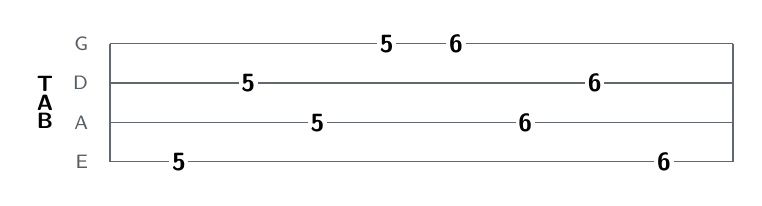
\begin{tikzpicture}[x=1cm,y=0.50cm]
\node[font=\sffamily\bfseries\footnotesize,align=center] at (-0.82,1.50) {T\\[-1mm]A\\[-1mm]B};
\foreach \y/\s in {3/G,2/D,1/A,0/E} {\draw[Ink!70,line width=0.55pt] (0,\y) -- (7.920,\y); \node[anchor=east,font=\sffamily\scriptsize,text=Ink!75] at (-0.15,\y) {\s};}
\draw[Ink!70,line width=0.7pt] (0,0) -- (0,3);
\draw[Ink!70,line width=0.7pt] (7.920,0) -- (7.920,3);
\node[fill=white,inner sep=1.0pt,font=\sffamily\bfseries\small] at (0.880,0) {5};
\node[fill=white,inner sep=1.0pt,font=\sffamily\bfseries\small] at (1.760,2) {5};
\node[fill=white,inner sep=1.0pt,font=\sffamily\bfseries\small] at (2.640,1) {5};
\node[fill=white,inner sep=1.0pt,font=\sffamily\bfseries\small] at (3.520,3) {5};
\node[fill=white,inner sep=1.0pt,font=\sffamily\bfseries\small] at (4.400,3) {6};
\node[fill=white,inner sep=1.0pt,font=\sffamily\bfseries\small] at (5.280,1) {6};
\node[fill=white,inner sep=1.0pt,font=\sffamily\bfseries\small] at (6.160,2) {6};
\node[fill=white,inner sep=1.0pt,font=\sffamily\bfseries\small] at (7.040,0) {6};
\end{tikzpicture}
\endgroup
\end{center}
\begin{tabularx}{\textwidth}{>{\bfseries\sffamily}p{3.0cm}Y}
Target & Skipped strings remain completely silent. \\
Progression & Begin at the lower tempo. Add 4 bpm after three clean repetitions; reduce by 6--8 bpm when timing or muting breaks down. \\
\end{tabularx}
\clearpage
\subsection{P9 - Two-fret position shift}\label{ex:p9}
\begin{keybox}
\textbf{Five-minute block.} Quarter note = 45--90 bpm; eighth notes.\\
\textbf{Play:} Play frets 5--8, then shift the entire hand to frets 7--10 without pausing.
\end{keybox}
\begin{center}
{\sffamily\bfseries\small Fretboard}\par\vspace{1mm}
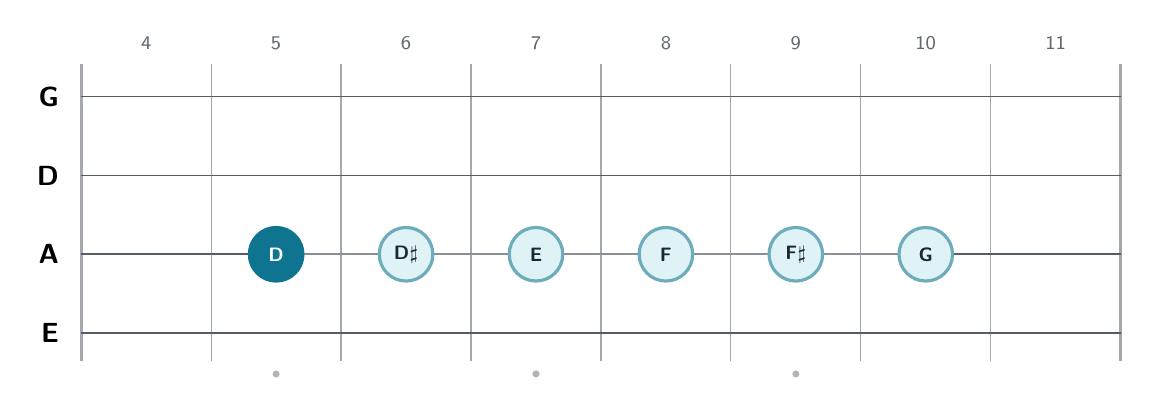
\begin{tikzpicture}[x=1cm,y=1cm,>=stealth]
\node[font=\sffamily\scriptsize,text=Ink!70] at (0.825,4.18) {4};
\node[font=\sffamily\scriptsize,text=Ink!70] at (2.475,4.18) {5};
\node[font=\sffamily\scriptsize,text=Ink!70] at (4.125,4.18) {6};
\node[font=\sffamily\scriptsize,text=Ink!70] at (5.775,4.18) {7};
\node[font=\sffamily\scriptsize,text=Ink!70] at (7.425,4.18) {8};
\node[font=\sffamily\scriptsize,text=Ink!70] at (9.075,4.18) {9};
\node[font=\sffamily\scriptsize,text=Ink!70] at (10.725,4.18) {10};
\node[font=\sffamily\scriptsize,text=Ink!70] at (12.375,4.18) {11};
\draw[Ink!40,line width=1.0pt] (0.000,0.15) -- (0.000,3.92);
\draw[Ink!40,line width=0.45pt] (1.650,0.15) -- (1.650,3.92);
\draw[Ink!40,line width=0.45pt] (3.300,0.15) -- (3.300,3.92);
\draw[Ink!40,line width=0.45pt] (4.950,0.15) -- (4.950,3.92);
\draw[Ink!40,line width=0.45pt] (6.600,0.15) -- (6.600,3.92);
\draw[Ink!40,line width=0.45pt] (8.250,0.15) -- (8.250,3.92);
\draw[Ink!40,line width=0.45pt] (9.900,0.15) -- (9.900,3.92);
\draw[Ink!40,line width=0.45pt] (11.550,0.15) -- (11.550,3.92);
\draw[Ink!40,line width=1.0pt] (13.200,0.15) -- (13.200,3.92);
\node[anchor=east,font=\sffamily\bfseries] at (-0.16,3.50) {G};
\draw[Ink!75,line width=0.45pt] (0,3.50) -- (13.200,3.50);
\node[anchor=east,font=\sffamily\bfseries] at (-0.16,2.50) {D};
\draw[Ink!75,line width=0.6pt] (0,2.50) -- (13.200,2.50);
\node[anchor=east,font=\sffamily\bfseries] at (-0.16,1.50) {A};
\draw[Ink!75,line width=0.8pt] (0,1.50) -- (13.200,1.50);
\node[anchor=east,font=\sffamily\bfseries] at (-0.16,0.50) {E};
\draw[Ink!75,line width=1.0pt] (0,0.50) -- (13.200,0.50);
\fill[Ink!35] (2.475,-0.02) circle (0.045);
\fill[Ink!35] (5.775,-0.02) circle (0.045);
\fill[Ink!35] (9.075,-0.02) circle (0.045);
\draw[->,Ink!52,line width=0.65pt] (2.475,1.500) -- (4.125,1.500);
\draw[->,Ink!52,line width=0.65pt] (4.125,1.500) -- (5.775,1.500);
\draw[->,Ink!52,line width=0.65pt] (5.775,1.500) -- (7.425,1.500);
\draw[->,Ink!52,line width=0.65pt] (7.425,1.500) -- (9.075,1.500);
\draw[->,Ink!52,line width=0.65pt] (9.075,1.500) -- (10.725,1.500);
\node[circle,minimum size=0.68cm,inner sep=0pt,fill=Accent,draw=Accent,text=white,line width=1.15pt,font=\sffamily\bfseries\scriptsize] at (2.475,1.500) {D};
\node[circle,minimum size=0.68cm,inner sep=0pt,fill=AccentLight,draw=Accent!60,text=Ink,line width=1.15pt,font=\sffamily\bfseries\scriptsize] at (4.125,1.500) {D$\sharp$};
\node[circle,minimum size=0.68cm,inner sep=0pt,fill=AccentLight,draw=Accent!60,text=Ink,line width=1.15pt,font=\sffamily\bfseries\scriptsize] at (5.775,1.500) {E};
\node[circle,minimum size=0.68cm,inner sep=0pt,fill=AccentLight,draw=Accent!60,text=Ink,line width=1.15pt,font=\sffamily\bfseries\scriptsize] at (7.425,1.500) {F};
\node[circle,minimum size=0.68cm,inner sep=0pt,fill=AccentLight,draw=Accent!60,text=Ink,line width=1.15pt,font=\sffamily\bfseries\scriptsize] at (9.075,1.500) {F$\sharp$};
\node[circle,minimum size=0.68cm,inner sep=0pt,fill=AccentLight,draw=Accent!60,text=Ink,line width=1.15pt,font=\sffamily\bfseries\scriptsize] at (10.725,1.500) {G};
\end{tikzpicture}
\end{center}
\begin{center}
\begingroup
\setlength{\parindent}{0pt}
\begin{minipage}{0.88\textwidth}
{\sffamily\bfseries\small Standard notation}\par\vspace{-1mm}
\begin{music}
\instrumentnumber{1}
\setstaffs1{1}
\setclef1{\bass}
\generalmeter{\meterfrac44}
\nobarnumbers
\nostartrule
\startextract
\Notes\cu{K}\cu{^K}\cu{L}\cu{M}\cu{L}\cu{M}\cu{^M}\cu{N}\en
\zendextract
\end{music}
\end{minipage}
\endgroup
\end{center}
\begin{center}
\begingroup
{\sffamily\bfseries\small Bass TAB}\par\vspace{1mm}
\begin{tikzpicture}[x=1cm,y=0.50cm]
\node[font=\sffamily\bfseries\footnotesize,align=center] at (-0.82,1.50) {T\\[-1mm]A\\[-1mm]B};
\foreach \y/\s in {3/G,2/D,1/A,0/E} {\draw[Ink!70,line width=0.55pt] (0,\y) -- (7.920,\y); \node[anchor=east,font=\sffamily\scriptsize,text=Ink!75] at (-0.15,\y) {\s};}
\draw[Ink!70,line width=0.7pt] (0,0) -- (0,3);
\draw[Ink!70,line width=0.7pt] (7.920,0) -- (7.920,3);
\node[fill=white,inner sep=1.0pt,font=\sffamily\bfseries\small] at (0.880,1) {5};
\node[fill=white,inner sep=1.0pt,font=\sffamily\bfseries\small] at (1.760,1) {6};
\node[fill=white,inner sep=1.0pt,font=\sffamily\bfseries\small] at (2.640,1) {7};
\node[fill=white,inner sep=1.0pt,font=\sffamily\bfseries\small] at (3.520,1) {8};
\node[fill=white,inner sep=1.0pt,font=\sffamily\bfseries\small] at (4.400,1) {7};
\node[fill=white,inner sep=1.0pt,font=\sffamily\bfseries\small] at (5.280,1) {8};
\node[fill=white,inner sep=1.0pt,font=\sffamily\bfseries\small] at (6.160,1) {9};
\node[fill=white,inner sep=1.0pt,font=\sffamily\bfseries\small] at (7.040,1) {10};
\end{tikzpicture}
\endgroup
\end{center}
\begin{tabularx}{\textwidth}{>{\bfseries\sffamily}p{3.0cm}Y}
Target & The shift lands exactly on fret 7 without an audible slide unless deliberately added. \\
Progression & Begin at the lower tempo. Add 4 bpm after three clean repetitions; reduce by 6--8 bpm when timing or muting breaks down. \\
\end{tabularx}
\clearpage
\subsection{P10 - Whole-position string shift}\label{ex:p10}
\begin{keybox}
\textbf{Five-minute block.} Quarter note = 45--95 bpm; eighth notes.\\
\textbf{Play:} Ascend across the strings at fret 5, shift to fret 7, and descend.
\end{keybox}
\begin{center}
{\sffamily\bfseries\small Fretboard}\par\vspace{1mm}
\begin{tikzpicture}[x=1cm,y=1cm,>=stealth]
\node[font=\sffamily\scriptsize,text=Ink!70] at (0.825,4.18) {4};
\node[font=\sffamily\scriptsize,text=Ink!70] at (2.475,4.18) {5};
\node[font=\sffamily\scriptsize,text=Ink!70] at (4.125,4.18) {6};
\node[font=\sffamily\scriptsize,text=Ink!70] at (5.775,4.18) {7};
\node[font=\sffamily\scriptsize,text=Ink!70] at (7.425,4.18) {8};
\draw[Ink!40,line width=1.0pt] (0.000,0.15) -- (0.000,3.92);
\draw[Ink!40,line width=0.45pt] (1.650,0.15) -- (1.650,3.92);
\draw[Ink!40,line width=0.45pt] (3.300,0.15) -- (3.300,3.92);
\draw[Ink!40,line width=0.45pt] (4.950,0.15) -- (4.950,3.92);
\draw[Ink!40,line width=0.45pt] (6.600,0.15) -- (6.600,3.92);
\draw[Ink!40,line width=1.0pt] (8.250,0.15) -- (8.250,3.92);
\node[anchor=east,font=\sffamily\bfseries] at (-0.16,3.50) {G};
\draw[Ink!75,line width=0.45pt] (0,3.50) -- (8.250,3.50);
\node[anchor=east,font=\sffamily\bfseries] at (-0.16,2.50) {D};
\draw[Ink!75,line width=0.6pt] (0,2.50) -- (8.250,2.50);
\node[anchor=east,font=\sffamily\bfseries] at (-0.16,1.50) {A};
\draw[Ink!75,line width=0.8pt] (0,1.50) -- (8.250,1.50);
\node[anchor=east,font=\sffamily\bfseries] at (-0.16,0.50) {E};
\draw[Ink!75,line width=1.0pt] (0,0.50) -- (8.250,0.50);
\fill[Ink!35] (2.475,-0.02) circle (0.045);
\fill[Ink!35] (5.775,-0.02) circle (0.045);
\draw[->,Ink!52,line width=0.65pt] (2.475,0.500) -- (2.475,1.500);
\draw[->,Ink!52,line width=0.65pt] (2.475,1.500) -- (2.475,2.500);
\draw[->,Ink!52,line width=0.65pt] (2.475,2.500) -- (2.475,3.500);
\draw[->,Ink!52,line width=0.65pt] (2.475,3.500) -- (5.775,3.500);
\draw[->,Ink!52,line width=0.65pt] (5.775,3.500) -- (5.775,2.500);
\draw[->,Ink!52,line width=0.65pt] (5.775,2.500) -- (5.775,1.500);
\draw[->,Ink!52,line width=0.65pt] (5.775,1.500) -- (5.775,0.500);
\node[circle,minimum size=0.68cm,inner sep=0pt,fill=Accent,draw=Accent,text=white,line width=1.15pt,font=\sffamily\bfseries\scriptsize] at (2.475,0.500) {A};
\node[circle,minimum size=0.68cm,inner sep=0pt,fill=AccentLight,draw=Accent!60,text=Ink,line width=1.15pt,font=\sffamily\bfseries\scriptsize] at (2.475,1.500) {D};
\node[circle,minimum size=0.68cm,inner sep=0pt,fill=AccentLight,draw=Accent!60,text=Ink,line width=1.15pt,font=\sffamily\bfseries\scriptsize] at (2.475,2.500) {G};
\node[circle,minimum size=0.68cm,inner sep=0pt,fill=AccentLight,draw=Accent!60,text=Ink,line width=1.15pt,font=\sffamily\bfseries\scriptsize] at (2.475,3.500) {C};
\node[circle,minimum size=0.68cm,inner sep=0pt,fill=AccentLight,draw=Accent!60,text=Ink,line width=1.15pt,font=\sffamily\bfseries\scriptsize] at (5.775,3.500) {D};
\node[circle,minimum size=0.68cm,inner sep=0pt,fill=Accent,draw=Accent,text=white,line width=1.15pt,font=\sffamily\bfseries\scriptsize] at (5.775,2.500) {A};
\node[circle,minimum size=0.68cm,inner sep=0pt,fill=AccentLight,draw=Accent!60,text=Ink,line width=1.15pt,font=\sffamily\bfseries\scriptsize] at (5.775,1.500) {E};
\node[circle,minimum size=0.68cm,inner sep=0pt,fill=AccentLight,draw=Accent!60,text=Ink,line width=1.15pt,font=\sffamily\bfseries\scriptsize] at (5.775,0.500) {B};
\end{tikzpicture}
\end{center}
\begin{center}
\begingroup
\setlength{\parindent}{0pt}
\begin{minipage}{0.88\textwidth}
{\sffamily\bfseries\small Standard notation}\par\vspace{-1mm}
\begin{music}
\instrumentnumber{1}
\setstaffs1{1}
\setclef1{\bass}
\generalmeter{\meterfrac44}
\nobarnumbers
\nostartrule
\startextract
\Notes\cu{H}\cu{K}\cu{N}\cu{c}\cu{d}\cu{a}\cu{L}\cu{I}\en
\zendextract
\end{music}
\end{minipage}
\endgroup
\end{center}
\begin{center}
\begingroup
{\sffamily\bfseries\small Bass TAB}\par\vspace{1mm}
\begin{tikzpicture}[x=1cm,y=0.50cm]
\node[font=\sffamily\bfseries\footnotesize,align=center] at (-0.82,1.50) {T\\[-1mm]A\\[-1mm]B};
\foreach \y/\s in {3/G,2/D,1/A,0/E} {\draw[Ink!70,line width=0.55pt] (0,\y) -- (7.920,\y); \node[anchor=east,font=\sffamily\scriptsize,text=Ink!75] at (-0.15,\y) {\s};}
\draw[Ink!70,line width=0.7pt] (0,0) -- (0,3);
\draw[Ink!70,line width=0.7pt] (7.920,0) -- (7.920,3);
\node[fill=white,inner sep=1.0pt,font=\sffamily\bfseries\small] at (0.880,0) {5};
\node[fill=white,inner sep=1.0pt,font=\sffamily\bfseries\small] at (1.760,1) {5};
\node[fill=white,inner sep=1.0pt,font=\sffamily\bfseries\small] at (2.640,2) {5};
\node[fill=white,inner sep=1.0pt,font=\sffamily\bfseries\small] at (3.520,3) {5};
\node[fill=white,inner sep=1.0pt,font=\sffamily\bfseries\small] at (4.400,3) {7};
\node[fill=white,inner sep=1.0pt,font=\sffamily\bfseries\small] at (5.280,2) {7};
\node[fill=white,inner sep=1.0pt,font=\sffamily\bfseries\small] at (6.160,1) {7};
\node[fill=white,inner sep=1.0pt,font=\sffamily\bfseries\small] at (7.040,0) {7};
\end{tikzpicture}
\endgroup
\end{center}
\begin{tabularx}{\textwidth}{>{\bfseries\sffamily}p{3.0cm}Y}
Target & The left hand shifts as one unit; right-hand alternation does not restart. \\
Progression & Begin at the lower tempo. Add 4 bpm after three clean repetitions; reduce by 6--8 bpm when timing or muting breaks down. \\
\end{tabularx}
\clearpage
\subsection{P11 - Movable octave shapes}\label{ex:p11}
\begin{keybox}
\textbf{Five-minute block.} Quarter note = 50--100 bpm; eighth notes.\\
\textbf{Play:} Play each low note followed by its octave two strings higher and two frets forward.
\end{keybox}
\begin{center}
{\sffamily\bfseries\small Fretboard}\par\vspace{1mm}
\begin{tikzpicture}[x=1cm,y=1cm,>=stealth]
\node[font=\sffamily\scriptsize,text=Ink!70] at (0.685,4.18) {4};
\node[font=\sffamily\scriptsize,text=Ink!70] at (2.055,4.18) {5};
\node[font=\sffamily\scriptsize,text=Ink!70] at (3.425,4.18) {6};
\node[font=\sffamily\scriptsize,text=Ink!70] at (4.795,4.18) {7};
\node[font=\sffamily\scriptsize,text=Ink!70] at (6.165,4.18) {8};
\node[font=\sffamily\scriptsize,text=Ink!70] at (7.535,4.18) {9};
\node[font=\sffamily\scriptsize,text=Ink!70] at (8.905,4.18) {10};
\node[font=\sffamily\scriptsize,text=Ink!70] at (10.275,4.18) {11};
\node[font=\sffamily\scriptsize,text=Ink!70] at (11.645,4.18) {12};
\node[font=\sffamily\scriptsize,text=Ink!70] at (13.015,4.18) {13};
\draw[Ink!40,line width=1.0pt] (0.000,0.15) -- (0.000,3.92);
\draw[Ink!40,line width=0.45pt] (1.370,0.15) -- (1.370,3.92);
\draw[Ink!40,line width=0.45pt] (2.740,0.15) -- (2.740,3.92);
\draw[Ink!40,line width=0.45pt] (4.110,0.15) -- (4.110,3.92);
\draw[Ink!40,line width=0.45pt] (5.480,0.15) -- (5.480,3.92);
\draw[Ink!40,line width=0.45pt] (6.850,0.15) -- (6.850,3.92);
\draw[Ink!40,line width=0.45pt] (8.220,0.15) -- (8.220,3.92);
\draw[Ink!40,line width=0.45pt] (9.590,0.15) -- (9.590,3.92);
\draw[Ink!40,line width=0.45pt] (10.960,0.15) -- (10.960,3.92);
\draw[Ink!40,line width=0.45pt] (12.330,0.15) -- (12.330,3.92);
\draw[Ink!40,line width=1.0pt] (13.700,0.15) -- (13.700,3.92);
\node[anchor=east,font=\sffamily\bfseries] at (-0.16,3.50) {G};
\draw[Ink!75,line width=0.45pt] (0,3.50) -- (13.700,3.50);
\node[anchor=east,font=\sffamily\bfseries] at (-0.16,2.50) {D};
\draw[Ink!75,line width=0.6pt] (0,2.50) -- (13.700,2.50);
\node[anchor=east,font=\sffamily\bfseries] at (-0.16,1.50) {A};
\draw[Ink!75,line width=0.8pt] (0,1.50) -- (13.700,1.50);
\node[anchor=east,font=\sffamily\bfseries] at (-0.16,0.50) {E};
\draw[Ink!75,line width=1.0pt] (0,0.50) -- (13.700,0.50);
\fill[Ink!35] (2.055,-0.02) circle (0.045);
\fill[Ink!35] (4.795,-0.02) circle (0.045);
\fill[Ink!35] (7.535,-0.02) circle (0.045);
\fill[Ink!35] (11.645,-0.02) circle (0.045);
\node[circle,minimum size=0.68cm,inner sep=0pt,fill=Accent,draw=Accent,text=white,line width=1.15pt,font=\sffamily\bfseries\scriptsize] at (2.055,0.500) {A};
\node[circle,minimum size=0.68cm,inner sep=0pt,fill=Accent,draw=Accent,text=white,line width=1.15pt,font=\sffamily\bfseries\scriptsize] at (4.795,2.500) {A};
\node[circle,minimum size=0.68cm,inner sep=0pt,fill=AccentLight,draw=Accent!60,text=Ink,line width=1.15pt,font=\sffamily\bfseries\scriptsize] at (4.795,0.500) {B};
\node[circle,minimum size=0.68cm,inner sep=0pt,fill=AccentLight,draw=Accent!60,text=Ink,line width=1.15pt,font=\sffamily\bfseries\scriptsize] at (7.535,2.500) {B};
\node[circle,minimum size=0.68cm,inner sep=0pt,fill=AccentLight,draw=Accent!60,text=Ink,line width=1.15pt,font=\sffamily\bfseries\scriptsize] at (6.165,0.500) {C};
\node[circle,minimum size=0.68cm,inner sep=0pt,fill=AccentLight,draw=Accent!60,text=Ink,line width=1.15pt,font=\sffamily\bfseries\scriptsize] at (8.905,2.500) {C};
\node[circle,minimum size=0.68cm,inner sep=0pt,fill=AccentLight,draw=Accent!60,text=Ink,line width=1.15pt,font=\sffamily\bfseries\scriptsize] at (8.905,0.500) {D};
\node[circle,minimum size=0.68cm,inner sep=0pt,fill=AccentLight,draw=Accent!60,text=Ink,line width=1.15pt,font=\sffamily\bfseries\scriptsize] at (11.645,2.500) {D};
\end{tikzpicture}
\end{center}
\begin{center}
\begingroup
\setlength{\parindent}{0pt}
\begin{minipage}{0.88\textwidth}
{\sffamily\bfseries\small Standard notation}\par\vspace{-1mm}
\begin{music}
\instrumentnumber{1}
\setstaffs1{1}
\setclef1{\bass}
\generalmeter{\meterfrac44}
\nobarnumbers
\nostartrule
\startextract
\Notes\cu{H}\cu{a}\cu{I}\cu{b}\cu{J}\cu{c}\cu{K}\cu{d}\en
\zendextract
\end{music}
\end{minipage}
\endgroup
\end{center}
\begin{center}
\begingroup
{\sffamily\bfseries\small Bass TAB}\par\vspace{1mm}
\begin{tikzpicture}[x=1cm,y=0.50cm]
\node[font=\sffamily\bfseries\footnotesize,align=center] at (-0.82,1.50) {T\\[-1mm]A\\[-1mm]B};
\foreach \y/\s in {3/G,2/D,1/A,0/E} {\draw[Ink!70,line width=0.55pt] (0,\y) -- (7.920,\y); \node[anchor=east,font=\sffamily\scriptsize,text=Ink!75] at (-0.15,\y) {\s};}
\draw[Ink!70,line width=0.7pt] (0,0) -- (0,3);
\draw[Ink!70,line width=0.7pt] (7.920,0) -- (7.920,3);
\node[fill=white,inner sep=1.0pt,font=\sffamily\bfseries\small] at (0.880,0) {5};
\node[fill=white,inner sep=1.0pt,font=\sffamily\bfseries\small] at (1.760,2) {7};
\node[fill=white,inner sep=1.0pt,font=\sffamily\bfseries\small] at (2.640,0) {7};
\node[fill=white,inner sep=1.0pt,font=\sffamily\bfseries\small] at (3.520,2) {9};
\node[fill=white,inner sep=1.0pt,font=\sffamily\bfseries\small] at (4.400,0) {8};
\node[fill=white,inner sep=1.0pt,font=\sffamily\bfseries\small] at (5.280,2) {10};
\node[fill=white,inner sep=1.0pt,font=\sffamily\bfseries\small] at (6.160,0) {10};
\node[fill=white,inner sep=1.0pt,font=\sffamily\bfseries\small] at (7.040,2) {12};
\end{tikzpicture}
\endgroup
\end{center}
\begin{tabularx}{\textwidth}{>{\bfseries\sffamily}p{3.0cm}Y}
Target & Both notes of every octave pair match in pitch identity and volume. \\
Progression & Begin at the lower tempo. Add 4 bpm after three clean repetitions; reduce by 6--8 bpm when timing or muting breaks down. \\
\end{tabularx}
\clearpage
\subsection{P12 - Root-fifth-octave triangle}\label{ex:p12}
\begin{keybox}
\textbf{Five-minute block.} Quarter note = 55--110 bpm; eighth notes.\\
\textbf{Play:} Cycle root--fifth--octave--fifth. Move the shape to G and A after one minute each.
\end{keybox}
\begin{center}
{\sffamily\bfseries\small Fretboard}\par\vspace{1mm}
\begin{tikzpicture}[x=1cm,y=1cm,>=stealth]
\node[font=\sffamily\scriptsize,text=Ink!70] at (0.825,4.18) {4};
\node[font=\sffamily\scriptsize,text=Ink!70] at (2.475,4.18) {5};
\node[font=\sffamily\scriptsize,text=Ink!70] at (4.125,4.18) {6};
\node[font=\sffamily\scriptsize,text=Ink!70] at (5.775,4.18) {7};
\node[font=\sffamily\scriptsize,text=Ink!70] at (7.425,4.18) {8};
\draw[Ink!40,line width=1.0pt] (0.000,0.15) -- (0.000,3.92);
\draw[Ink!40,line width=0.45pt] (1.650,0.15) -- (1.650,3.92);
\draw[Ink!40,line width=0.45pt] (3.300,0.15) -- (3.300,3.92);
\draw[Ink!40,line width=0.45pt] (4.950,0.15) -- (4.950,3.92);
\draw[Ink!40,line width=0.45pt] (6.600,0.15) -- (6.600,3.92);
\draw[Ink!40,line width=1.0pt] (8.250,0.15) -- (8.250,3.92);
\node[anchor=east,font=\sffamily\bfseries] at (-0.16,3.50) {G};
\draw[Ink!75,line width=0.45pt] (0,3.50) -- (8.250,3.50);
\node[anchor=east,font=\sffamily\bfseries] at (-0.16,2.50) {D};
\draw[Ink!75,line width=0.6pt] (0,2.50) -- (8.250,2.50);
\node[anchor=east,font=\sffamily\bfseries] at (-0.16,1.50) {A};
\draw[Ink!75,line width=0.8pt] (0,1.50) -- (8.250,1.50);
\node[anchor=east,font=\sffamily\bfseries] at (-0.16,0.50) {E};
\draw[Ink!75,line width=1.0pt] (0,0.50) -- (8.250,0.50);
\fill[Ink!35] (2.475,-0.02) circle (0.045);
\fill[Ink!35] (5.775,-0.02) circle (0.045);
\draw[->,Ink!52,line width=0.65pt] (2.475,1.500) -- (5.775,2.500);
\draw[->,Ink!52,line width=0.65pt] (5.775,2.500) -- (5.775,3.500);
\node[circle,minimum size=0.68cm,inner sep=0pt,fill=Accent,draw=Accent,text=white,line width=1.15pt,font=\sffamily\bfseries\scriptsize] at (2.475,1.500) {D};
\node[circle,minimum size=0.68cm,inner sep=0pt,fill=AccentLight,draw=Accent!60,text=Ink,line width=1.15pt,font=\sffamily\bfseries\scriptsize] at (5.775,2.500) {A};
\node[circle,minimum size=0.68cm,inner sep=0pt,fill=Accent,draw=Accent,text=white,line width=1.15pt,font=\sffamily\bfseries\scriptsize] at (5.775,3.500) {D};
\end{tikzpicture}
\end{center}
\begin{center}
\begingroup
\setlength{\parindent}{0pt}
\begin{minipage}{0.88\textwidth}
{\sffamily\bfseries\small Standard notation}\par\vspace{-1mm}
\begin{music}
\instrumentnumber{1}
\setstaffs1{1}
\setclef1{\bass}
\generalmeter{\meterfrac44}
\nobarnumbers
\nostartrule
\startextract
\Notes\cu{K}\cu{a}\cu{d}\cu{a}\cu{K}\cu{a}\cu{d}\cu{K}\en
\zendextract
\end{music}
\end{minipage}
\endgroup
\end{center}
\begin{center}
\begingroup
{\sffamily\bfseries\small Bass TAB}\par\vspace{1mm}
\begin{tikzpicture}[x=1cm,y=0.50cm]
\node[font=\sffamily\bfseries\footnotesize,align=center] at (-0.82,1.50) {T\\[-1mm]A\\[-1mm]B};
\foreach \y/\s in {3/G,2/D,1/A,0/E} {\draw[Ink!70,line width=0.55pt] (0,\y) -- (7.920,\y); \node[anchor=east,font=\sffamily\scriptsize,text=Ink!75] at (-0.15,\y) {\s};}
\draw[Ink!70,line width=0.7pt] (0,0) -- (0,3);
\draw[Ink!70,line width=0.7pt] (7.920,0) -- (7.920,3);
\node[fill=white,inner sep=1.0pt,font=\sffamily\bfseries\small] at (0.880,1) {5};
\node[fill=white,inner sep=1.0pt,font=\sffamily\bfseries\small] at (1.760,2) {7};
\node[fill=white,inner sep=1.0pt,font=\sffamily\bfseries\small] at (2.640,3) {7};
\node[fill=white,inner sep=1.0pt,font=\sffamily\bfseries\small] at (3.520,2) {7};
\node[fill=white,inner sep=1.0pt,font=\sffamily\bfseries\small] at (4.400,1) {5};
\node[fill=white,inner sep=1.0pt,font=\sffamily\bfseries\small] at (5.280,2) {7};
\node[fill=white,inner sep=1.0pt,font=\sffamily\bfseries\small] at (6.160,3) {7};
\node[fill=white,inner sep=1.0pt,font=\sffamily\bfseries\small] at (7.040,1) {5};
\end{tikzpicture}
\endgroup
\end{center}
\begin{tabularx}{\textwidth}{>{\bfseries\sffamily}p{3.0cm}Y}
Target & String crossings sound connected without notes overlapping. \\
Progression & Begin at the lower tempo. Add 4 bpm after three clean repetitions; reduce by 6--8 bpm when timing or muting breaks down. \\
\end{tabularx}
\clearpage
\subsection{P13 - Minor-third and major-third control}\label{ex:p13}
\begin{keybox}
\textbf{Five-minute block.} Quarter note = 50--95 bpm; eighth notes.\\
\textbf{Play:} Alternate the minor third and major third above D. Use fingers that keep the hand relaxed.
\end{keybox}
\begin{center}
{\sffamily\bfseries\small Fretboard}\par\vspace{1mm}
\begin{tikzpicture}[x=1cm,y=1cm,>=stealth]
\node[font=\sffamily\scriptsize,text=Ink!70] at (0.825,4.18) {2};
\node[font=\sffamily\scriptsize,text=Ink!70] at (2.475,4.18) {3};
\node[font=\sffamily\scriptsize,text=Ink!70] at (4.125,4.18) {4};
\node[font=\sffamily\scriptsize,text=Ink!70] at (5.775,4.18) {5};
\node[font=\sffamily\scriptsize,text=Ink!70] at (7.425,4.18) {6};
\draw[Ink!40,line width=1.0pt] (0.000,0.15) -- (0.000,3.92);
\draw[Ink!40,line width=0.45pt] (1.650,0.15) -- (1.650,3.92);
\draw[Ink!40,line width=0.45pt] (3.300,0.15) -- (3.300,3.92);
\draw[Ink!40,line width=0.45pt] (4.950,0.15) -- (4.950,3.92);
\draw[Ink!40,line width=0.45pt] (6.600,0.15) -- (6.600,3.92);
\draw[Ink!40,line width=1.0pt] (8.250,0.15) -- (8.250,3.92);
\node[anchor=east,font=\sffamily\bfseries] at (-0.16,3.50) {G};
\draw[Ink!75,line width=0.45pt] (0,3.50) -- (8.250,3.50);
\node[anchor=east,font=\sffamily\bfseries] at (-0.16,2.50) {D};
\draw[Ink!75,line width=0.6pt] (0,2.50) -- (8.250,2.50);
\node[anchor=east,font=\sffamily\bfseries] at (-0.16,1.50) {A};
\draw[Ink!75,line width=0.8pt] (0,1.50) -- (8.250,1.50);
\node[anchor=east,font=\sffamily\bfseries] at (-0.16,0.50) {E};
\draw[Ink!75,line width=1.0pt] (0,0.50) -- (8.250,0.50);
\fill[Ink!35] (2.475,-0.02) circle (0.045);
\fill[Ink!35] (5.775,-0.02) circle (0.045);
\draw[->,Ink!52,line width=0.65pt] (5.775,1.500) -- (2.475,2.500);
\draw[->,Ink!52,line width=0.65pt] (2.475,2.500) -- (4.125,2.500);
\node[circle,minimum size=0.68cm,inner sep=0pt,fill=Accent,draw=Accent,text=white,line width=1.15pt,font=\sffamily\bfseries\scriptsize] at (5.775,1.500) {D};
\node[circle,minimum size=0.68cm,inner sep=0pt,fill=AccentLight,draw=Accent!60,text=Ink,line width=1.15pt,font=\sffamily\bfseries\scriptsize] at (2.475,2.500) {F};
\node[circle,minimum size=0.68cm,inner sep=0pt,fill=AccentLight,draw=Accent!60,text=Ink,line width=1.15pt,font=\sffamily\bfseries\scriptsize] at (4.125,2.500) {F$\sharp$};
\end{tikzpicture}
\end{center}
\begin{center}
\begingroup
\setlength{\parindent}{0pt}
\begin{minipage}{0.88\textwidth}
{\sffamily\bfseries\small Standard notation}\par\vspace{-1mm}
\begin{music}
\instrumentnumber{1}
\setstaffs1{1}
\setclef1{\bass}
\generalmeter{\meterfrac44}
\nobarnumbers
\nostartrule
\startextract
\Notes\cu{K}\cu{M}\cu{^M}\cu{=M}\cu{K}\cu{^M}\cu{=M}\cu{K}\en
\zendextract
\end{music}
\end{minipage}
\endgroup
\end{center}
\begin{center}
\begingroup
{\sffamily\bfseries\small Bass TAB}\par\vspace{1mm}
\begin{tikzpicture}[x=1cm,y=0.50cm]
\node[font=\sffamily\bfseries\footnotesize,align=center] at (-0.82,1.50) {T\\[-1mm]A\\[-1mm]B};
\foreach \y/\s in {3/G,2/D,1/A,0/E} {\draw[Ink!70,line width=0.55pt] (0,\y) -- (7.920,\y); \node[anchor=east,font=\sffamily\scriptsize,text=Ink!75] at (-0.15,\y) {\s};}
\draw[Ink!70,line width=0.7pt] (0,0) -- (0,3);
\draw[Ink!70,line width=0.7pt] (7.920,0) -- (7.920,3);
\node[fill=white,inner sep=1.0pt,font=\sffamily\bfseries\small] at (0.880,1) {5};
\node[fill=white,inner sep=1.0pt,font=\sffamily\bfseries\small] at (1.760,2) {3};
\node[fill=white,inner sep=1.0pt,font=\sffamily\bfseries\small] at (2.640,2) {4};
\node[fill=white,inner sep=1.0pt,font=\sffamily\bfseries\small] at (3.520,2) {3};
\node[fill=white,inner sep=1.0pt,font=\sffamily\bfseries\small] at (4.400,1) {5};
\node[fill=white,inner sep=1.0pt,font=\sffamily\bfseries\small] at (5.280,2) {4};
\node[fill=white,inner sep=1.0pt,font=\sffamily\bfseries\small] at (6.160,2) {3};
\node[fill=white,inner sep=1.0pt,font=\sffamily\bfseries\small] at (7.040,1) {5};
\end{tikzpicture}
\endgroup
\end{center}
\begin{tabularx}{\textwidth}{>{\bfseries\sffamily}p{3.0cm}Y}
Target & The one-fret distinction is visually, physically and aurally clear. \\
Progression & Begin at the lower tempo. Add 4 bpm after three clean repetitions; reduce by 6--8 bpm when timing or muting breaks down. \\
\end{tabularx}
\clearpage
\subsection{P14 - One-fret diagonal crawl}\label{ex:p14}
\begin{keybox}
\textbf{Five-minute block.} Quarter note = 40--85 bpm; eighth notes.\\
\textbf{Play:} Move one fret higher with each higher string, then reverse by one fret per string.
\end{keybox}
\begin{center}
{\sffamily\bfseries\small Fretboard}\par\vspace{1mm}
\begin{tikzpicture}[x=1cm,y=1cm,>=stealth]
\node[font=\sffamily\scriptsize,text=Ink!70] at (0.825,4.18) {2};
\node[font=\sffamily\scriptsize,text=Ink!70] at (2.475,4.18) {3};
\node[font=\sffamily\scriptsize,text=Ink!70] at (4.125,4.18) {4};
\node[font=\sffamily\scriptsize,text=Ink!70] at (5.775,4.18) {5};
\node[font=\sffamily\scriptsize,text=Ink!70] at (7.425,4.18) {6};
\node[font=\sffamily\scriptsize,text=Ink!70] at (9.075,4.18) {7};
\node[font=\sffamily\scriptsize,text=Ink!70] at (10.725,4.18) {8};
\draw[Ink!40,line width=1.0pt] (0.000,0.15) -- (0.000,3.92);
\draw[Ink!40,line width=0.45pt] (1.650,0.15) -- (1.650,3.92);
\draw[Ink!40,line width=0.45pt] (3.300,0.15) -- (3.300,3.92);
\draw[Ink!40,line width=0.45pt] (4.950,0.15) -- (4.950,3.92);
\draw[Ink!40,line width=0.45pt] (6.600,0.15) -- (6.600,3.92);
\draw[Ink!40,line width=0.45pt] (8.250,0.15) -- (8.250,3.92);
\draw[Ink!40,line width=0.45pt] (9.900,0.15) -- (9.900,3.92);
\draw[Ink!40,line width=1.0pt] (11.550,0.15) -- (11.550,3.92);
\node[anchor=east,font=\sffamily\bfseries] at (-0.16,3.50) {G};
\draw[Ink!75,line width=0.45pt] (0,3.50) -- (11.550,3.50);
\node[anchor=east,font=\sffamily\bfseries] at (-0.16,2.50) {D};
\draw[Ink!75,line width=0.6pt] (0,2.50) -- (11.550,2.50);
\node[anchor=east,font=\sffamily\bfseries] at (-0.16,1.50) {A};
\draw[Ink!75,line width=0.8pt] (0,1.50) -- (11.550,1.50);
\node[anchor=east,font=\sffamily\bfseries] at (-0.16,0.50) {E};
\draw[Ink!75,line width=1.0pt] (0,0.50) -- (11.550,0.50);
\fill[Ink!35] (2.475,-0.02) circle (0.045);
\fill[Ink!35] (5.775,-0.02) circle (0.045);
\fill[Ink!35] (9.075,-0.02) circle (0.045);
\draw[->,Ink!52,line width=0.65pt] (4.125,0.500) -- (5.775,1.500);
\draw[->,Ink!52,line width=0.65pt] (5.775,1.500) -- (7.425,2.500);
\draw[->,Ink!52,line width=0.65pt] (7.425,2.500) -- (9.075,3.500);
\draw[->,Ink!52,line width=0.65pt] (9.075,3.500) -- (7.425,3.500);
\draw[->,Ink!52,line width=0.65pt] (7.425,3.500) -- (5.775,2.500);
\draw[->,Ink!52,line width=0.65pt] (5.775,2.500) -- (4.125,1.500);
\draw[->,Ink!52,line width=0.65pt] (4.125,1.500) -- (2.475,0.500);
\node[circle,minimum size=0.68cm,inner sep=0pt,fill=Accent,draw=Accent,text=white,line width=1.15pt,font=\sffamily\bfseries\scriptsize] at (4.125,0.500) {G$\sharp$};
\node[circle,minimum size=0.68cm,inner sep=0pt,fill=AccentLight,draw=Accent!60,text=Ink,line width=1.15pt,font=\sffamily\bfseries\scriptsize] at (5.775,1.500) {D};
\node[circle,minimum size=0.68cm,inner sep=0pt,fill=Accent,draw=Accent,text=white,line width=1.15pt,font=\sffamily\bfseries\scriptsize] at (7.425,2.500) {G$\sharp$};
\node[circle,minimum size=0.68cm,inner sep=0pt,fill=AccentLight,draw=Accent!60,text=Ink,line width=1.15pt,font=\sffamily\bfseries\scriptsize] at (9.075,3.500) {D};
\node[circle,minimum size=0.68cm,inner sep=0pt,fill=AccentLight,draw=Accent!60,text=Ink,line width=1.15pt,font=\sffamily\bfseries\scriptsize] at (7.425,3.500) {C$\sharp$};
\node[circle,minimum size=0.68cm,inner sep=0pt,fill=AccentLight,draw=Accent!60,text=Ink,line width=1.15pt,font=\sffamily\bfseries\scriptsize] at (5.775,2.500) {G};
\node[circle,minimum size=0.68cm,inner sep=0pt,fill=AccentLight,draw=Accent!60,text=Ink,line width=1.15pt,font=\sffamily\bfseries\scriptsize] at (4.125,1.500) {C$\sharp$};
\node[circle,minimum size=0.68cm,inner sep=0pt,fill=AccentLight,draw=Accent!60,text=Ink,line width=1.15pt,font=\sffamily\bfseries\scriptsize] at (2.475,0.500) {G};
\end{tikzpicture}
\end{center}
\begin{center}
\begingroup
\setlength{\parindent}{0pt}
\begin{minipage}{0.88\textwidth}
{\sffamily\bfseries\small Standard notation}\par\vspace{-1mm}
\begin{music}
\instrumentnumber{1}
\setstaffs1{1}
\setclef1{\bass}
\generalmeter{\meterfrac44}
\nobarnumbers
\nostartrule
\startextract
\Notes\cu{^G}\cu{K}\cu{N}\cu{d}\cu{^c}\cu{=N}\cu{J}\cu{G}\en
\zendextract
\end{music}
\end{minipage}
\endgroup
\end{center}
\begin{center}
\begingroup
{\sffamily\bfseries\small Bass TAB}\par\vspace{1mm}
\begin{tikzpicture}[x=1cm,y=0.50cm]
\node[font=\sffamily\bfseries\footnotesize,align=center] at (-0.82,1.50) {T\\[-1mm]A\\[-1mm]B};
\foreach \y/\s in {3/G,2/D,1/A,0/E} {\draw[Ink!70,line width=0.55pt] (0,\y) -- (7.920,\y); \node[anchor=east,font=\sffamily\scriptsize,text=Ink!75] at (-0.15,\y) {\s};}
\draw[Ink!70,line width=0.7pt] (0,0) -- (0,3);
\draw[Ink!70,line width=0.7pt] (7.920,0) -- (7.920,3);
\node[fill=white,inner sep=1.0pt,font=\sffamily\bfseries\small] at (0.880,0) {4};
\node[fill=white,inner sep=1.0pt,font=\sffamily\bfseries\small] at (1.760,1) {5};
\node[fill=white,inner sep=1.0pt,font=\sffamily\bfseries\small] at (2.640,2) {6};
\node[fill=white,inner sep=1.0pt,font=\sffamily\bfseries\small] at (3.520,3) {7};
\node[fill=white,inner sep=1.0pt,font=\sffamily\bfseries\small] at (4.400,3) {6};
\node[fill=white,inner sep=1.0pt,font=\sffamily\bfseries\small] at (5.280,2) {5};
\node[fill=white,inner sep=1.0pt,font=\sffamily\bfseries\small] at (6.160,1) {4};
\node[fill=white,inner sep=1.0pt,font=\sffamily\bfseries\small] at (7.040,0) {3};
\end{tikzpicture}
\endgroup
\end{center}
\begin{tabularx}{\textwidth}{>{\bfseries\sffamily}p{3.0cm}Y}
Target & Finger placement stays immediately behind each fret. \\
Progression & Begin at the lower tempo. Add 4 bpm after three clean repetitions; reduce by 6--8 bpm when timing or muting breaks down. \\
\end{tabularx}
\clearpage
\subsection{P15 - Three-notes-per-string coordination}\label{ex:p15}
\begin{keybox}
\textbf{Five-minute block.} Quarter note = 50--105 bpm; eighth notes.\\
\textbf{Play:} Use the D-major fingering but treat it as a coordination drill. Reverse after the octave.
\end{keybox}
\begin{center}
{\sffamily\bfseries\small Fretboard}\par\vspace{1mm}
\begin{tikzpicture}[x=1cm,y=1cm,>=stealth]
\node[font=\sffamily\scriptsize,text=Ink!70] at (0.825,4.18) {4};
\node[font=\sffamily\scriptsize,text=Ink!70] at (2.475,4.18) {5};
\node[font=\sffamily\scriptsize,text=Ink!70] at (4.125,4.18) {6};
\node[font=\sffamily\scriptsize,text=Ink!70] at (5.775,4.18) {7};
\node[font=\sffamily\scriptsize,text=Ink!70] at (7.425,4.18) {8};
\node[font=\sffamily\scriptsize,text=Ink!70] at (9.075,4.18) {9};
\node[font=\sffamily\scriptsize,text=Ink!70] at (10.725,4.18) {10};
\draw[Ink!40,line width=1.0pt] (0.000,0.15) -- (0.000,3.92);
\draw[Ink!40,line width=0.45pt] (1.650,0.15) -- (1.650,3.92);
\draw[Ink!40,line width=0.45pt] (3.300,0.15) -- (3.300,3.92);
\draw[Ink!40,line width=0.45pt] (4.950,0.15) -- (4.950,3.92);
\draw[Ink!40,line width=0.45pt] (6.600,0.15) -- (6.600,3.92);
\draw[Ink!40,line width=0.45pt] (8.250,0.15) -- (8.250,3.92);
\draw[Ink!40,line width=0.45pt] (9.900,0.15) -- (9.900,3.92);
\draw[Ink!40,line width=1.0pt] (11.550,0.15) -- (11.550,3.92);
\node[anchor=east,font=\sffamily\bfseries] at (-0.16,3.50) {G};
\draw[Ink!75,line width=0.45pt] (0,3.50) -- (11.550,3.50);
\node[anchor=east,font=\sffamily\bfseries] at (-0.16,2.50) {D};
\draw[Ink!75,line width=0.6pt] (0,2.50) -- (11.550,2.50);
\node[anchor=east,font=\sffamily\bfseries] at (-0.16,1.50) {A};
\draw[Ink!75,line width=0.8pt] (0,1.50) -- (11.550,1.50);
\node[anchor=east,font=\sffamily\bfseries] at (-0.16,0.50) {E};
\draw[Ink!75,line width=1.0pt] (0,0.50) -- (11.550,0.50);
\fill[Ink!35] (2.475,-0.02) circle (0.045);
\fill[Ink!35] (5.775,-0.02) circle (0.045);
\fill[Ink!35] (9.075,-0.02) circle (0.045);
\draw[->,Ink!52,line width=0.65pt] (2.475,1.500) -- (5.775,1.500);
\draw[->,Ink!52,line width=0.65pt] (5.775,1.500) -- (9.075,1.500);
\draw[->,Ink!52,line width=0.65pt] (9.075,1.500) -- (2.475,2.500);
\draw[->,Ink!52,line width=0.65pt] (2.475,2.500) -- (5.775,2.500);
\draw[->,Ink!52,line width=0.65pt] (5.775,2.500) -- (9.075,2.500);
\draw[->,Ink!52,line width=0.65pt] (9.075,2.500) -- (4.125,3.500);
\draw[->,Ink!52,line width=0.65pt] (4.125,3.500) -- (5.775,3.500);
\node[circle,minimum size=0.68cm,inner sep=0pt,fill=Accent,draw=Accent,text=white,line width=1.15pt,font=\sffamily\bfseries\scriptsize] at (2.475,1.500) {D};
\node[circle,minimum size=0.68cm,inner sep=0pt,fill=AccentLight,draw=Accent!60,text=Ink,line width=1.15pt,font=\sffamily\bfseries\scriptsize] at (5.775,1.500) {E};
\node[circle,minimum size=0.68cm,inner sep=0pt,fill=AccentLight,draw=Accent!60,text=Ink,line width=1.15pt,font=\sffamily\bfseries\scriptsize] at (9.075,1.500) {F$\sharp$};
\node[circle,minimum size=0.68cm,inner sep=0pt,fill=AccentLight,draw=Accent!60,text=Ink,line width=1.15pt,font=\sffamily\bfseries\scriptsize] at (2.475,2.500) {G};
\node[circle,minimum size=0.68cm,inner sep=0pt,fill=AccentLight,draw=Accent!60,text=Ink,line width=1.15pt,font=\sffamily\bfseries\scriptsize] at (5.775,2.500) {A};
\node[circle,minimum size=0.68cm,inner sep=0pt,fill=AccentLight,draw=Accent!60,text=Ink,line width=1.15pt,font=\sffamily\bfseries\scriptsize] at (9.075,2.500) {B};
\node[circle,minimum size=0.68cm,inner sep=0pt,fill=AccentLight,draw=Accent!60,text=Ink,line width=1.15pt,font=\sffamily\bfseries\scriptsize] at (4.125,3.500) {C$\sharp$};
\node[circle,minimum size=0.68cm,inner sep=0pt,fill=Accent,draw=Accent,text=white,line width=1.15pt,font=\sffamily\bfseries\scriptsize] at (5.775,3.500) {D};
\end{tikzpicture}
\end{center}
\begin{center}
\begingroup
\setlength{\parindent}{0pt}
\begin{minipage}{0.88\textwidth}
{\sffamily\bfseries\small Standard notation}\par\vspace{-1mm}
\begin{music}
\instrumentnumber{1}
\setstaffs1{1}
\setclef1{\bass}
\generalmeter{\meterfrac44}
\nobarnumbers
\nostartrule
\startextract
\Notes\cu{K}\cu{L}\cu{^M}\cu{N}\cu{a}\cu{b}\cu{^c}\cu{d}\en
\zendextract
\end{music}
\end{minipage}
\endgroup
\end{center}
\begin{center}
\begingroup
{\sffamily\bfseries\small Bass TAB}\par\vspace{1mm}
\begin{tikzpicture}[x=1cm,y=0.50cm]
\node[font=\sffamily\bfseries\footnotesize,align=center] at (-0.82,1.50) {T\\[-1mm]A\\[-1mm]B};
\foreach \y/\s in {3/G,2/D,1/A,0/E} {\draw[Ink!70,line width=0.55pt] (0,\y) -- (7.920,\y); \node[anchor=east,font=\sffamily\scriptsize,text=Ink!75] at (-0.15,\y) {\s};}
\draw[Ink!70,line width=0.7pt] (0,0) -- (0,3);
\draw[Ink!70,line width=0.7pt] (7.920,0) -- (7.920,3);
\node[fill=white,inner sep=1.0pt,font=\sffamily\bfseries\small] at (0.880,1) {5};
\node[fill=white,inner sep=1.0pt,font=\sffamily\bfseries\small] at (1.760,1) {7};
\node[fill=white,inner sep=1.0pt,font=\sffamily\bfseries\small] at (2.640,1) {9};
\node[fill=white,inner sep=1.0pt,font=\sffamily\bfseries\small] at (3.520,2) {5};
\node[fill=white,inner sep=1.0pt,font=\sffamily\bfseries\small] at (4.400,2) {7};
\node[fill=white,inner sep=1.0pt,font=\sffamily\bfseries\small] at (5.280,2) {9};
\node[fill=white,inner sep=1.0pt,font=\sffamily\bfseries\small] at (6.160,3) {6};
\node[fill=white,inner sep=1.0pt,font=\sffamily\bfseries\small] at (7.040,3) {7};
\end{tikzpicture}
\endgroup
\end{center}
\begin{tabularx}{\textwidth}{>{\bfseries\sffamily}p{3.0cm}Y}
Target & String changes do not disturb the eighth-note pulse. \\
Progression & Begin at the lower tempo. Add 4 bpm after three clean repetitions; reduce by 6--8 bpm when timing or muting breaks down. \\
\end{tabularx}
\clearpage
\subsection{P16 - Repeated-note plucking alternation}\label{ex:p16}
\begin{keybox}
\textbf{Five-minute block.} Quarter note = 60--140 bpm; eighth notes.\\
\textbf{Play:} Play one D repeatedly with strict index-middle alternation. Start the next repetition with the opposite finger.
\end{keybox}
\begin{center}
{\sffamily\bfseries\small Fretboard}\par\vspace{1mm}
\begin{tikzpicture}[x=1cm,y=1cm,>=stealth]
\node[font=\sffamily\scriptsize,text=Ink!70] at (0.825,4.18) {4};
\node[font=\sffamily\scriptsize,text=Ink!70] at (2.475,4.18) {5};
\node[font=\sffamily\scriptsize,text=Ink!70] at (4.125,4.18) {6};
\draw[Ink!40,line width=1.0pt] (0.000,0.15) -- (0.000,3.92);
\draw[Ink!40,line width=0.45pt] (1.650,0.15) -- (1.650,3.92);
\draw[Ink!40,line width=0.45pt] (3.300,0.15) -- (3.300,3.92);
\draw[Ink!40,line width=1.0pt] (4.950,0.15) -- (4.950,3.92);
\node[anchor=east,font=\sffamily\bfseries] at (-0.16,3.50) {G};
\draw[Ink!75,line width=0.45pt] (0,3.50) -- (4.950,3.50);
\node[anchor=east,font=\sffamily\bfseries] at (-0.16,2.50) {D};
\draw[Ink!75,line width=0.6pt] (0,2.50) -- (4.950,2.50);
\node[anchor=east,font=\sffamily\bfseries] at (-0.16,1.50) {A};
\draw[Ink!75,line width=0.8pt] (0,1.50) -- (4.950,1.50);
\node[anchor=east,font=\sffamily\bfseries] at (-0.16,0.50) {E};
\draw[Ink!75,line width=1.0pt] (0,0.50) -- (4.950,0.50);
\fill[Ink!35] (2.475,-0.02) circle (0.045);
\node[circle,minimum size=0.68cm,inner sep=0pt,fill=Accent,draw=Accent,text=white,line width=1.15pt,font=\sffamily\bfseries\scriptsize] at (2.475,1.500) {D};
\end{tikzpicture}
\end{center}
\begin{center}
\begingroup
\setlength{\parindent}{0pt}
\begin{minipage}{0.88\textwidth}
{\sffamily\bfseries\small Standard notation}\par\vspace{-1mm}
\begin{music}
\instrumentnumber{1}
\setstaffs1{1}
\setclef1{\bass}
\generalmeter{\meterfrac44}
\nobarnumbers
\nostartrule
\startextract
\Notes\cu{K}\cu{K}\cu{K}\cu{K}\cu{K}\cu{K}\cu{K}\cu{K}\en
\zendextract
\end{music}
\end{minipage}
\endgroup
\end{center}
\begin{center}
\begingroup
{\sffamily\bfseries\small Bass TAB}\par\vspace{1mm}
\begin{tikzpicture}[x=1cm,y=0.50cm]
\node[font=\sffamily\bfseries\footnotesize,align=center] at (-0.82,1.50) {T\\[-1mm]A\\[-1mm]B};
\foreach \y/\s in {3/G,2/D,1/A,0/E} {\draw[Ink!70,line width=0.55pt] (0,\y) -- (7.920,\y); \node[anchor=east,font=\sffamily\scriptsize,text=Ink!75] at (-0.15,\y) {\s};}
\draw[Ink!70,line width=0.7pt] (0,0) -- (0,3);
\draw[Ink!70,line width=0.7pt] (7.920,0) -- (7.920,3);
\node[fill=white,inner sep=1.0pt,font=\sffamily\bfseries\small] at (0.880,1) {5};
\node[fill=white,inner sep=1.0pt,font=\sffamily\bfseries\small] at (1.760,1) {5};
\node[fill=white,inner sep=1.0pt,font=\sffamily\bfseries\small] at (2.640,1) {5};
\node[fill=white,inner sep=1.0pt,font=\sffamily\bfseries\small] at (3.520,1) {5};
\node[fill=white,inner sep=1.0pt,font=\sffamily\bfseries\small] at (4.400,1) {5};
\node[fill=white,inner sep=1.0pt,font=\sffamily\bfseries\small] at (5.280,1) {5};
\node[fill=white,inner sep=1.0pt,font=\sffamily\bfseries\small] at (6.160,1) {5};
\node[fill=white,inner sep=1.0pt,font=\sffamily\bfseries\small] at (7.040,1) {5};
\end{tikzpicture}
\endgroup
\end{center}
\begin{tabularx}{\textwidth}{>{\bfseries\sffamily}p{3.0cm}Y}
Target & No change in tone, volume or timing between plucking fingers. \\
Progression & Begin at the lower tempo. Add 4 bpm after three clean repetitions; reduce by 6--8 bpm when timing or muting breaks down. \\
\end{tabularx}
\clearpage
\subsection{P17 - Two-string alternation}\label{ex:p17}
\begin{keybox}
\textbf{Five-minute block.} Quarter note = 55--125 bpm; eighth notes.\\
\textbf{Play:} Alternate A and D strings while maintaining index-middle alternation.
\end{keybox}
\begin{center}
{\sffamily\bfseries\small Fretboard}\par\vspace{1mm}
\begin{tikzpicture}[x=1cm,y=1cm,>=stealth]
\node[font=\sffamily\scriptsize,text=Ink!70] at (0.825,4.18) {4};
\node[font=\sffamily\scriptsize,text=Ink!70] at (2.475,4.18) {5};
\node[font=\sffamily\scriptsize,text=Ink!70] at (4.125,4.18) {6};
\draw[Ink!40,line width=1.0pt] (0.000,0.15) -- (0.000,3.92);
\draw[Ink!40,line width=0.45pt] (1.650,0.15) -- (1.650,3.92);
\draw[Ink!40,line width=0.45pt] (3.300,0.15) -- (3.300,3.92);
\draw[Ink!40,line width=1.0pt] (4.950,0.15) -- (4.950,3.92);
\node[anchor=east,font=\sffamily\bfseries] at (-0.16,3.50) {G};
\draw[Ink!75,line width=0.45pt] (0,3.50) -- (4.950,3.50);
\node[anchor=east,font=\sffamily\bfseries] at (-0.16,2.50) {D};
\draw[Ink!75,line width=0.6pt] (0,2.50) -- (4.950,2.50);
\node[anchor=east,font=\sffamily\bfseries] at (-0.16,1.50) {A};
\draw[Ink!75,line width=0.8pt] (0,1.50) -- (4.950,1.50);
\node[anchor=east,font=\sffamily\bfseries] at (-0.16,0.50) {E};
\draw[Ink!75,line width=1.0pt] (0,0.50) -- (4.950,0.50);
\fill[Ink!35] (2.475,-0.02) circle (0.045);
\node[circle,minimum size=0.68cm,inner sep=0pt,fill=Accent,draw=Accent,text=white,line width=1.15pt,font=\sffamily\bfseries\scriptsize] at (2.475,1.500) {D};
\node[circle,minimum size=0.68cm,inner sep=0pt,fill=AccentLight,draw=Accent!60,text=Ink,line width=1.15pt,font=\sffamily\bfseries\scriptsize] at (2.475,2.500) {G};
\end{tikzpicture}
\end{center}
\begin{center}
\begingroup
\setlength{\parindent}{0pt}
\begin{minipage}{0.88\textwidth}
{\sffamily\bfseries\small Standard notation}\par\vspace{-1mm}
\begin{music}
\instrumentnumber{1}
\setstaffs1{1}
\setclef1{\bass}
\generalmeter{\meterfrac44}
\nobarnumbers
\nostartrule
\startextract
\Notes\cu{K}\cu{N}\cu{K}\cu{N}\cu{K}\cu{N}\cu{K}\cu{N}\en
\zendextract
\end{music}
\end{minipage}
\endgroup
\end{center}
\begin{center}
\begingroup
{\sffamily\bfseries\small Bass TAB}\par\vspace{1mm}
\begin{tikzpicture}[x=1cm,y=0.50cm]
\node[font=\sffamily\bfseries\footnotesize,align=center] at (-0.82,1.50) {T\\[-1mm]A\\[-1mm]B};
\foreach \y/\s in {3/G,2/D,1/A,0/E} {\draw[Ink!70,line width=0.55pt] (0,\y) -- (7.920,\y); \node[anchor=east,font=\sffamily\scriptsize,text=Ink!75] at (-0.15,\y) {\s};}
\draw[Ink!70,line width=0.7pt] (0,0) -- (0,3);
\draw[Ink!70,line width=0.7pt] (7.920,0) -- (7.920,3);
\node[fill=white,inner sep=1.0pt,font=\sffamily\bfseries\small] at (0.880,1) {5};
\node[fill=white,inner sep=1.0pt,font=\sffamily\bfseries\small] at (1.760,2) {5};
\node[fill=white,inner sep=1.0pt,font=\sffamily\bfseries\small] at (2.640,1) {5};
\node[fill=white,inner sep=1.0pt,font=\sffamily\bfseries\small] at (3.520,2) {5};
\node[fill=white,inner sep=1.0pt,font=\sffamily\bfseries\small] at (4.400,1) {5};
\node[fill=white,inner sep=1.0pt,font=\sffamily\bfseries\small] at (5.280,2) {5};
\node[fill=white,inner sep=1.0pt,font=\sffamily\bfseries\small] at (6.160,1) {5};
\node[fill=white,inner sep=1.0pt,font=\sffamily\bfseries\small] at (7.040,2) {5};
\end{tikzpicture}
\endgroup
\end{center}
\begin{tabularx}{\textwidth}{>{\bfseries\sffamily}p{3.0cm}Y}
Target & The lower string is muted immediately after each change. \\
Progression & Begin at the lower tempo. Add 4 bpm after three clean repetitions; reduce by 6--8 bpm when timing or muting breaks down. \\
\end{tabularx}
\clearpage
\subsection{P18 - Wide string-skip control}\label{ex:p18}
\begin{keybox}
\textbf{Five-minute block.} Quarter note = 40--90 bpm; eighth notes.\\
\textbf{Play:} Alternate between E and G strings. Keep A and D muted throughout.
\end{keybox}
\begin{center}
{\sffamily\bfseries\small Fretboard}\par\vspace{1mm}
\begin{tikzpicture}[x=1cm,y=1cm,>=stealth]
\node[font=\sffamily\scriptsize,text=Ink!70] at (0.825,4.18) {4};
\node[font=\sffamily\scriptsize,text=Ink!70] at (2.475,4.18) {5};
\node[font=\sffamily\scriptsize,text=Ink!70] at (4.125,4.18) {6};
\node[font=\sffamily\scriptsize,text=Ink!70] at (5.775,4.18) {7};
\node[font=\sffamily\scriptsize,text=Ink!70] at (7.425,4.18) {8};
\node[font=\sffamily\scriptsize,text=Ink!70] at (9.075,4.18) {9};
\node[font=\sffamily\scriptsize,text=Ink!70] at (10.725,4.18) {10};
\node[font=\sffamily\scriptsize,text=Ink!70] at (12.375,4.18) {11};
\draw[Ink!40,line width=1.0pt] (0.000,0.15) -- (0.000,3.92);
\draw[Ink!40,line width=0.45pt] (1.650,0.15) -- (1.650,3.92);
\draw[Ink!40,line width=0.45pt] (3.300,0.15) -- (3.300,3.92);
\draw[Ink!40,line width=0.45pt] (4.950,0.15) -- (4.950,3.92);
\draw[Ink!40,line width=0.45pt] (6.600,0.15) -- (6.600,3.92);
\draw[Ink!40,line width=0.45pt] (8.250,0.15) -- (8.250,3.92);
\draw[Ink!40,line width=0.45pt] (9.900,0.15) -- (9.900,3.92);
\draw[Ink!40,line width=0.45pt] (11.550,0.15) -- (11.550,3.92);
\draw[Ink!40,line width=1.0pt] (13.200,0.15) -- (13.200,3.92);
\node[anchor=east,font=\sffamily\bfseries] at (-0.16,3.50) {G};
\draw[Ink!75,line width=0.45pt] (0,3.50) -- (13.200,3.50);
\node[anchor=east,font=\sffamily\bfseries] at (-0.16,2.50) {D};
\draw[Ink!75,line width=0.6pt] (0,2.50) -- (13.200,2.50);
\node[anchor=east,font=\sffamily\bfseries] at (-0.16,1.50) {A};
\draw[Ink!75,line width=0.8pt] (0,1.50) -- (13.200,1.50);
\node[anchor=east,font=\sffamily\bfseries] at (-0.16,0.50) {E};
\draw[Ink!75,line width=1.0pt] (0,0.50) -- (13.200,0.50);
\fill[Ink!35] (2.475,-0.02) circle (0.045);
\fill[Ink!35] (5.775,-0.02) circle (0.045);
\fill[Ink!35] (9.075,-0.02) circle (0.045);
\draw[->,Ink!52,line width=0.65pt] (2.475,0.500) -- (2.475,3.500);
\draw[->,Ink!52,line width=0.65pt] (2.475,3.500) -- (5.775,0.500);
\draw[->,Ink!52,line width=0.65pt] (5.775,0.500) -- (5.775,3.500);
\draw[->,Ink!52,line width=0.65pt] (5.775,3.500) -- (7.425,0.500);
\draw[->,Ink!52,line width=0.65pt] (7.425,0.500) -- (7.425,3.500);
\draw[->,Ink!52,line width=0.65pt] (7.425,3.500) -- (10.725,0.500);
\draw[->,Ink!52,line width=0.65pt] (10.725,0.500) -- (10.725,3.500);
\node[circle,minimum size=0.68cm,inner sep=0pt,fill=Accent,draw=Accent,text=white,line width=1.15pt,font=\sffamily\bfseries\scriptsize] at (2.475,0.500) {A};
\node[circle,minimum size=0.68cm,inner sep=0pt,fill=AccentLight,draw=Accent!60,text=Ink,line width=1.15pt,font=\sffamily\bfseries\scriptsize] at (2.475,3.500) {C};
\node[circle,minimum size=0.68cm,inner sep=0pt,fill=AccentLight,draw=Accent!60,text=Ink,line width=1.15pt,font=\sffamily\bfseries\scriptsize] at (5.775,0.500) {B};
\node[circle,minimum size=0.68cm,inner sep=0pt,fill=AccentLight,draw=Accent!60,text=Ink,line width=1.15pt,font=\sffamily\bfseries\scriptsize] at (5.775,3.500) {D};
\node[circle,minimum size=0.68cm,inner sep=0pt,fill=AccentLight,draw=Accent!60,text=Ink,line width=1.15pt,font=\sffamily\bfseries\scriptsize] at (7.425,0.500) {C};
\node[circle,minimum size=0.68cm,inner sep=0pt,fill=AccentLight,draw=Accent!60,text=Ink,line width=1.15pt,font=\sffamily\bfseries\scriptsize] at (7.425,3.500) {D$\sharp$};
\node[circle,minimum size=0.68cm,inner sep=0pt,fill=AccentLight,draw=Accent!60,text=Ink,line width=1.15pt,font=\sffamily\bfseries\scriptsize] at (10.725,0.500) {D};
\node[circle,minimum size=0.68cm,inner sep=0pt,fill=AccentLight,draw=Accent!60,text=Ink,line width=1.15pt,font=\sffamily\bfseries\scriptsize] at (10.725,3.500) {F};
\end{tikzpicture}
\end{center}
\begin{center}
\begingroup
\setlength{\parindent}{0pt}
\begin{minipage}{0.88\textwidth}
{\sffamily\bfseries\small Standard notation}\par\vspace{-1mm}
\begin{music}
\instrumentnumber{1}
\setstaffs1{1}
\setclef1{\bass}
\generalmeter{\meterfrac44}
\nobarnumbers
\nostartrule
\startextract
\Notes\cu{H}\cu{c}\cu{I}\cu{d}\cu{J}\cu{^d}\cu{=K}\cu{f}\en
\zendextract
\end{music}
\end{minipage}
\endgroup
\end{center}
\begin{center}
\begingroup
{\sffamily\bfseries\small Bass TAB}\par\vspace{1mm}
\begin{tikzpicture}[x=1cm,y=0.50cm]
\node[font=\sffamily\bfseries\footnotesize,align=center] at (-0.82,1.50) {T\\[-1mm]A\\[-1mm]B};
\foreach \y/\s in {3/G,2/D,1/A,0/E} {\draw[Ink!70,line width=0.55pt] (0,\y) -- (7.920,\y); \node[anchor=east,font=\sffamily\scriptsize,text=Ink!75] at (-0.15,\y) {\s};}
\draw[Ink!70,line width=0.7pt] (0,0) -- (0,3);
\draw[Ink!70,line width=0.7pt] (7.920,0) -- (7.920,3);
\node[fill=white,inner sep=1.0pt,font=\sffamily\bfseries\small] at (0.880,0) {5};
\node[fill=white,inner sep=1.0pt,font=\sffamily\bfseries\small] at (1.760,3) {5};
\node[fill=white,inner sep=1.0pt,font=\sffamily\bfseries\small] at (2.640,0) {7};
\node[fill=white,inner sep=1.0pt,font=\sffamily\bfseries\small] at (3.520,3) {7};
\node[fill=white,inner sep=1.0pt,font=\sffamily\bfseries\small] at (4.400,0) {8};
\node[fill=white,inner sep=1.0pt,font=\sffamily\bfseries\small] at (5.280,3) {8};
\node[fill=white,inner sep=1.0pt,font=\sffamily\bfseries\small] at (6.160,0) {10};
\node[fill=white,inner sep=1.0pt,font=\sffamily\bfseries\small] at (7.040,3) {10};
\end{tikzpicture}
\endgroup
\end{center}
\begin{tabularx}{\textwidth}{>{\bfseries\sffamily}p{3.0cm}Y}
Target & The attack remains centered despite the two-string leap. \\
Progression & Begin at the lower tempo. Add 4 bpm after three clean repetitions; reduce by 6--8 bpm when timing or muting breaks down. \\
\end{tabularx}
\clearpage
\subsection{P19 - Hammer-on and pull-off cell}\label{ex:p19}
\begin{keybox}
\textbf{Five-minute block.} Quarter note = 45--90 bpm; eighth notes.\\
\textbf{Play:} Pluck the first note of each four-note group; use hammer-ons and pull-offs for the remaining notes.
\end{keybox}
\begin{center}
{\sffamily\bfseries\small Fretboard}\par\vspace{1mm}
\begin{tikzpicture}[x=1cm,y=1cm,>=stealth]
\node[font=\sffamily\scriptsize,text=Ink!70] at (0.825,4.18) {4};
\node[font=\sffamily\scriptsize,text=Ink!70] at (2.475,4.18) {5};
\node[font=\sffamily\scriptsize,text=Ink!70] at (4.125,4.18) {6};
\node[font=\sffamily\scriptsize,text=Ink!70] at (5.775,4.18) {7};
\node[font=\sffamily\scriptsize,text=Ink!70] at (7.425,4.18) {8};
\node[font=\sffamily\scriptsize,text=Ink!70] at (9.075,4.18) {9};
\draw[Ink!40,line width=1.0pt] (0.000,0.15) -- (0.000,3.92);
\draw[Ink!40,line width=0.45pt] (1.650,0.15) -- (1.650,3.92);
\draw[Ink!40,line width=0.45pt] (3.300,0.15) -- (3.300,3.92);
\draw[Ink!40,line width=0.45pt] (4.950,0.15) -- (4.950,3.92);
\draw[Ink!40,line width=0.45pt] (6.600,0.15) -- (6.600,3.92);
\draw[Ink!40,line width=0.45pt] (8.250,0.15) -- (8.250,3.92);
\draw[Ink!40,line width=1.0pt] (9.900,0.15) -- (9.900,3.92);
\node[anchor=east,font=\sffamily\bfseries] at (-0.16,3.50) {G};
\draw[Ink!75,line width=0.45pt] (0,3.50) -- (9.900,3.50);
\node[anchor=east,font=\sffamily\bfseries] at (-0.16,2.50) {D};
\draw[Ink!75,line width=0.6pt] (0,2.50) -- (9.900,2.50);
\node[anchor=east,font=\sffamily\bfseries] at (-0.16,1.50) {A};
\draw[Ink!75,line width=0.8pt] (0,1.50) -- (9.900,1.50);
\node[anchor=east,font=\sffamily\bfseries] at (-0.16,0.50) {E};
\draw[Ink!75,line width=1.0pt] (0,0.50) -- (9.900,0.50);
\fill[Ink!35] (2.475,-0.02) circle (0.045);
\fill[Ink!35] (5.775,-0.02) circle (0.045);
\fill[Ink!35] (9.075,-0.02) circle (0.045);
\draw[->,Ink!52,line width=0.65pt] (2.475,1.500) -- (5.775,1.500);
\draw[->,Ink!52,line width=0.65pt] (5.775,1.500) -- (7.425,1.500);
\node[circle,minimum size=0.68cm,inner sep=0pt,fill=Accent,draw=Accent,text=white,line width=1.15pt,font=\sffamily\bfseries\scriptsize] at (2.475,1.500) {D};
\node[circle,minimum size=0.68cm,inner sep=0pt,fill=AccentLight,draw=Accent!60,text=Ink,line width=1.15pt,font=\sffamily\bfseries\scriptsize] at (5.775,1.500) {E};
\node[circle,minimum size=0.68cm,inner sep=0pt,fill=AccentLight,draw=Accent!60,text=Ink,line width=1.15pt,font=\sffamily\bfseries\scriptsize] at (7.425,1.500) {F};
\end{tikzpicture}
\end{center}
\begin{center}
\begingroup
\setlength{\parindent}{0pt}
\begin{minipage}{0.88\textwidth}
{\sffamily\bfseries\small Standard notation}\par\vspace{-1mm}
\begin{music}
\instrumentnumber{1}
\setstaffs1{1}
\setclef1{\bass}
\generalmeter{\meterfrac44}
\nobarnumbers
\nostartrule
\startextract
\Notes\cu{K}\cu{L}\cu{M}\cu{L}\cu{K}\cu{L}\cu{M}\cu{K}\en
\zendextract
\end{music}
\end{minipage}
\endgroup
\end{center}
\begin{center}
\begingroup
{\sffamily\bfseries\small Bass TAB}\par\vspace{1mm}
\begin{tikzpicture}[x=1cm,y=0.50cm]
\node[font=\sffamily\bfseries\footnotesize,align=center] at (-0.82,1.50) {T\\[-1mm]A\\[-1mm]B};
\foreach \y/\s in {3/G,2/D,1/A,0/E} {\draw[Ink!70,line width=0.55pt] (0,\y) -- (7.920,\y); \node[anchor=east,font=\sffamily\scriptsize,text=Ink!75] at (-0.15,\y) {\s};}
\draw[Ink!70,line width=0.7pt] (0,0) -- (0,3);
\draw[Ink!70,line width=0.7pt] (7.920,0) -- (7.920,3);
\node[fill=white,inner sep=1.0pt,font=\sffamily\bfseries\small] at (0.880,1) {5};
\node[fill=white,inner sep=1.0pt,font=\sffamily\bfseries\small] at (1.760,1) {7};
\node[fill=white,inner sep=1.0pt,font=\sffamily\bfseries\small] at (2.640,1) {8};
\node[fill=white,inner sep=1.0pt,font=\sffamily\bfseries\small] at (3.520,1) {7};
\node[fill=white,inner sep=1.0pt,font=\sffamily\bfseries\small] at (4.400,1) {5};
\node[fill=white,inner sep=1.0pt,font=\sffamily\bfseries\small] at (5.280,1) {7};
\node[fill=white,inner sep=1.0pt,font=\sffamily\bfseries\small] at (6.160,1) {8};
\node[fill=white,inner sep=1.0pt,font=\sffamily\bfseries\small] at (7.040,1) {5};
\end{tikzpicture}
\endgroup
\end{center}
\begin{tabularx}{\textwidth}{>{\bfseries\sffamily}p{3.0cm}Y}
Target & Legato notes match the plucked note in volume and rhythmic placement. \\
Progression & Begin at the lower tempo. Add 4 bpm after three clean repetitions; reduce by 6--8 bpm when timing or muting breaks down. \\
\end{tabularx}
\clearpage
\subsection{P20 - Four-string endurance pedal}\label{ex:p20}
\begin{keybox}
\textbf{Five-minute block.} Quarter note = 70--140 bpm; eighth notes.\\
\textbf{Play:} Play four repeated notes on each string without stopping. Reverse the string order on alternate repetitions.
\end{keybox}
\begin{center}
{\sffamily\bfseries\small Fretboard}\par\vspace{1mm}
\begin{tikzpicture}[x=1cm,y=1cm,>=stealth]
\node[font=\sffamily\scriptsize,text=Ink!70] at (0.825,4.18) {6};
\node[font=\sffamily\scriptsize,text=Ink!70] at (2.475,4.18) {7};
\node[font=\sffamily\scriptsize,text=Ink!70] at (4.125,4.18) {8};
\draw[Ink!40,line width=1.0pt] (0.000,0.15) -- (0.000,3.92);
\draw[Ink!40,line width=0.45pt] (1.650,0.15) -- (1.650,3.92);
\draw[Ink!40,line width=0.45pt] (3.300,0.15) -- (3.300,3.92);
\draw[Ink!40,line width=1.0pt] (4.950,0.15) -- (4.950,3.92);
\node[anchor=east,font=\sffamily\bfseries] at (-0.16,3.50) {G};
\draw[Ink!75,line width=0.45pt] (0,3.50) -- (4.950,3.50);
\node[anchor=east,font=\sffamily\bfseries] at (-0.16,2.50) {D};
\draw[Ink!75,line width=0.6pt] (0,2.50) -- (4.950,2.50);
\node[anchor=east,font=\sffamily\bfseries] at (-0.16,1.50) {A};
\draw[Ink!75,line width=0.8pt] (0,1.50) -- (4.950,1.50);
\node[anchor=east,font=\sffamily\bfseries] at (-0.16,0.50) {E};
\draw[Ink!75,line width=1.0pt] (0,0.50) -- (4.950,0.50);
\fill[Ink!35] (2.475,-0.02) circle (0.045);
\node[circle,minimum size=0.68cm,inner sep=0pt,fill=Accent,draw=Accent,text=white,line width=1.15pt,font=\sffamily\bfseries\scriptsize] at (2.475,0.500) {B};
\node[circle,minimum size=0.68cm,inner sep=0pt,fill=AccentLight,draw=Accent!60,text=Ink,line width=1.15pt,font=\sffamily\bfseries\scriptsize] at (2.475,1.500) {E};
\node[circle,minimum size=0.68cm,inner sep=0pt,fill=AccentLight,draw=Accent!60,text=Ink,line width=1.15pt,font=\sffamily\bfseries\scriptsize] at (2.475,2.500) {A};
\node[circle,minimum size=0.68cm,inner sep=0pt,fill=AccentLight,draw=Accent!60,text=Ink,line width=1.15pt,font=\sffamily\bfseries\scriptsize] at (2.475,3.500) {D};
\end{tikzpicture}
\end{center}
\begin{center}
\begingroup
\setlength{\parindent}{0pt}
\begin{minipage}{0.88\textwidth}
{\sffamily\bfseries\small Standard notation}\par\vspace{-1mm}
\begin{music}
\instrumentnumber{1}
\setstaffs1{1}
\setclef1{\bass}
\generalmeter{\meterfrac44}
\nobarnumbers
\nostartrule
\startextract
\Notes\cu{I}\cu{I}\cu{I}\cu{I}\cu{L}\cu{L}\cu{L}\cu{L}\en
\bar
\Notes\cu{a}\cu{a}\cu{a}\cu{a}\cu{d}\cu{d}\cu{d}\cu{d}\en
\zendextract
\end{music}
\end{minipage}
\endgroup
\end{center}
\begin{center}
\begingroup
{\sffamily\bfseries\small Bass TAB}\par\vspace{1mm}
\begin{tikzpicture}[x=1cm,y=0.50cm]
\node[font=\sffamily\bfseries\footnotesize,align=center] at (-0.82,1.50) {T\\[-1mm]A\\[-1mm]B};
\foreach \y/\s in {3/G,2/D,1/A,0/E} {\draw[Ink!70,line width=0.55pt] (0,\y) -- (13.200,\y); \node[anchor=east,font=\sffamily\scriptsize,text=Ink!75] at (-0.15,\y) {\s};}
\draw[Ink!70,line width=0.7pt] (0,0) -- (0,3);
\draw[Ink!70,line width=0.7pt] (13.200,0) -- (13.200,3);
\node[fill=white,inner sep=1.0pt,font=\sffamily\bfseries\small] at (0.776,0) {7};
\node[fill=white,inner sep=1.0pt,font=\sffamily\bfseries\small] at (1.553,0) {7};
\node[fill=white,inner sep=1.0pt,font=\sffamily\bfseries\small] at (2.329,0) {7};
\node[fill=white,inner sep=1.0pt,font=\sffamily\bfseries\small] at (3.106,0) {7};
\node[fill=white,inner sep=1.0pt,font=\sffamily\bfseries\small] at (3.882,1) {7};
\node[fill=white,inner sep=1.0pt,font=\sffamily\bfseries\small] at (4.659,1) {7};
\node[fill=white,inner sep=1.0pt,font=\sffamily\bfseries\small] at (5.435,1) {7};
\node[fill=white,inner sep=1.0pt,font=\sffamily\bfseries\small] at (6.212,1) {7};
\node[fill=white,inner sep=1.0pt,font=\sffamily\bfseries\small] at (6.988,2) {7};
\node[fill=white,inner sep=1.0pt,font=\sffamily\bfseries\small] at (7.765,2) {7};
\node[fill=white,inner sep=1.0pt,font=\sffamily\bfseries\small] at (8.541,2) {7};
\node[fill=white,inner sep=1.0pt,font=\sffamily\bfseries\small] at (9.318,2) {7};
\node[fill=white,inner sep=1.0pt,font=\sffamily\bfseries\small] at (10.094,3) {7};
\node[fill=white,inner sep=1.0pt,font=\sffamily\bfseries\small] at (10.871,3) {7};
\node[fill=white,inner sep=1.0pt,font=\sffamily\bfseries\small] at (11.647,3) {7};
\node[fill=white,inner sep=1.0pt,font=\sffamily\bfseries\small] at (12.424,3) {7};
\end{tikzpicture}
\endgroup
\end{center}
\begin{tabularx}{\textwidth}{>{\bfseries\sffamily}p{3.0cm}Y}
Target & Maintain relaxed hands and consistent sound for the full five minutes. \\
Progression & Begin at the lower tempo. Add 4 bpm after three clean repetitions; reduce by 6--8 bpm when timing or muting breaks down. \\
\end{tabularx}
\clearpage
\section{Musical control: 20 five-minute blocks}
\subsection{M1 - D major scale}\label{ex:m1}
\begin{keybox}
\textbf{Five-minute block.} Quarter note = 60--120 bpm; eighth notes.\\
\textbf{Play:} Play ascending, then reverse. Say either note names or degrees 1--2--3--4--5--6--7--8.
\end{keybox}
\begin{center}
{\sffamily\bfseries\small Fretboard}\par\vspace{1mm}
\begin{tikzpicture}[x=1cm,y=1cm,>=stealth]
\node[font=\sffamily\scriptsize,text=Ink!70] at (0.825,4.18) {4};
\node[font=\sffamily\scriptsize,text=Ink!70] at (2.475,4.18) {5};
\node[font=\sffamily\scriptsize,text=Ink!70] at (4.125,4.18) {6};
\node[font=\sffamily\scriptsize,text=Ink!70] at (5.775,4.18) {7};
\node[font=\sffamily\scriptsize,text=Ink!70] at (7.425,4.18) {8};
\node[font=\sffamily\scriptsize,text=Ink!70] at (9.075,4.18) {9};
\node[font=\sffamily\scriptsize,text=Ink!70] at (10.725,4.18) {10};
\draw[Ink!40,line width=1.0pt] (0.000,0.15) -- (0.000,3.92);
\draw[Ink!40,line width=0.45pt] (1.650,0.15) -- (1.650,3.92);
\draw[Ink!40,line width=0.45pt] (3.300,0.15) -- (3.300,3.92);
\draw[Ink!40,line width=0.45pt] (4.950,0.15) -- (4.950,3.92);
\draw[Ink!40,line width=0.45pt] (6.600,0.15) -- (6.600,3.92);
\draw[Ink!40,line width=0.45pt] (8.250,0.15) -- (8.250,3.92);
\draw[Ink!40,line width=0.45pt] (9.900,0.15) -- (9.900,3.92);
\draw[Ink!40,line width=1.0pt] (11.550,0.15) -- (11.550,3.92);
\node[anchor=east,font=\sffamily\bfseries] at (-0.16,3.50) {G};
\draw[Ink!75,line width=0.45pt] (0,3.50) -- (11.550,3.50);
\node[anchor=east,font=\sffamily\bfseries] at (-0.16,2.50) {D};
\draw[Ink!75,line width=0.6pt] (0,2.50) -- (11.550,2.50);
\node[anchor=east,font=\sffamily\bfseries] at (-0.16,1.50) {A};
\draw[Ink!75,line width=0.8pt] (0,1.50) -- (11.550,1.50);
\node[anchor=east,font=\sffamily\bfseries] at (-0.16,0.50) {E};
\draw[Ink!75,line width=1.0pt] (0,0.50) -- (11.550,0.50);
\fill[Ink!35] (2.475,-0.02) circle (0.045);
\fill[Ink!35] (5.775,-0.02) circle (0.045);
\fill[Ink!35] (9.075,-0.02) circle (0.045);
\draw[->,Ink!52,line width=0.65pt] (2.475,1.500) -- (5.775,1.500);
\draw[->,Ink!52,line width=0.65pt] (5.775,1.500) -- (9.075,1.500);
\draw[->,Ink!52,line width=0.65pt] (9.075,1.500) -- (2.475,2.500);
\draw[->,Ink!52,line width=0.65pt] (2.475,2.500) -- (5.775,2.500);
\draw[->,Ink!52,line width=0.65pt] (5.775,2.500) -- (9.075,2.500);
\draw[->,Ink!52,line width=0.65pt] (9.075,2.500) -- (4.125,3.500);
\draw[->,Ink!52,line width=0.65pt] (4.125,3.500) -- (5.775,3.500);
\node[circle,minimum size=0.68cm,inner sep=0pt,fill=Accent,draw=Accent,text=white,line width=1.15pt,font=\sffamily\bfseries\scriptsize] at (2.475,1.500) {D};
\node[circle,minimum size=0.68cm,inner sep=0pt,fill=AccentLight,draw=Accent!60,text=Ink,line width=1.15pt,font=\sffamily\bfseries\scriptsize] at (5.775,1.500) {E};
\node[circle,minimum size=0.68cm,inner sep=0pt,fill=ChordLight,draw=Chord,text=Ink,line width=1.15pt,font=\sffamily\bfseries\scriptsize] at (9.075,1.500) {F$\sharp$};
\node[circle,minimum size=0.68cm,inner sep=0pt,fill=AccentLight,draw=Accent!60,text=Ink,line width=1.15pt,font=\sffamily\bfseries\scriptsize] at (2.475,2.500) {G};
\node[circle,minimum size=0.68cm,inner sep=0pt,fill=ChordLight,draw=Chord,text=Ink,line width=1.15pt,font=\sffamily\bfseries\scriptsize] at (5.775,2.500) {A};
\node[circle,minimum size=0.68cm,inner sep=0pt,fill=AccentLight,draw=Accent!60,text=Ink,line width=1.15pt,font=\sffamily\bfseries\scriptsize] at (9.075,2.500) {B};
\node[circle,minimum size=0.68cm,inner sep=0pt,fill=ChordLight,draw=Chord,text=Ink,line width=1.15pt,font=\sffamily\bfseries\scriptsize] at (4.125,3.500) {C$\sharp$};
\node[circle,minimum size=0.68cm,inner sep=0pt,fill=Accent,draw=Accent,text=white,line width=1.15pt,font=\sffamily\bfseries\scriptsize] at (5.775,3.500) {D};
\end{tikzpicture}
\end{center}
\begin{center}
\begingroup
\setlength{\parindent}{0pt}
\begin{minipage}{0.88\textwidth}
{\sffamily\bfseries\small Standard notation}\par\vspace{-1mm}
\begin{music}
\instrumentnumber{1}
\setstaffs1{1}
\setclef1{\bass}
\generalmeter{\meterfrac44}
\nobarnumbers
\nostartrule
\startextract
\Notes\cu{K}\cu{L}\cu{^M}\cu{N}\cu{a}\cu{b}\cu{^c}\cu{d}\en
\zendextract
\end{music}
\end{minipage}
\endgroup
\end{center}
\begin{center}
\begingroup
{\sffamily\bfseries\small Bass TAB}\par\vspace{1mm}
\begin{tikzpicture}[x=1cm,y=0.50cm]
\node[font=\sffamily\bfseries\footnotesize,align=center] at (-0.82,1.50) {T\\[-1mm]A\\[-1mm]B};
\foreach \y/\s in {3/G,2/D,1/A,0/E} {\draw[Ink!70,line width=0.55pt] (0,\y) -- (7.920,\y); \node[anchor=east,font=\sffamily\scriptsize,text=Ink!75] at (-0.15,\y) {\s};}
\draw[Ink!70,line width=0.7pt] (0,0) -- (0,3);
\draw[Ink!70,line width=0.7pt] (7.920,0) -- (7.920,3);
\node[fill=white,inner sep=1.0pt,font=\sffamily\bfseries\small] at (0.880,1) {5};
\node[fill=white,inner sep=1.0pt,font=\sffamily\bfseries\small] at (1.760,1) {7};
\node[fill=white,inner sep=1.0pt,font=\sffamily\bfseries\small] at (2.640,1) {9};
\node[fill=white,inner sep=1.0pt,font=\sffamily\bfseries\small] at (3.520,2) {5};
\node[fill=white,inner sep=1.0pt,font=\sffamily\bfseries\small] at (4.400,2) {7};
\node[fill=white,inner sep=1.0pt,font=\sffamily\bfseries\small] at (5.280,2) {9};
\node[fill=white,inner sep=1.0pt,font=\sffamily\bfseries\small] at (6.160,3) {6};
\node[fill=white,inner sep=1.0pt,font=\sffamily\bfseries\small] at (7.040,3) {7};
\end{tikzpicture}
\endgroup
\end{center}
\begin{tabularx}{\textwidth}{>{\bfseries\sffamily}p{3.0cm}Y}
Target & Hear the half steps F-sharp--G and C-sharp--D. \\
Progression & Begin at the lower tempo. Add 4 bpm after three clean repetitions; reduce by 6--8 bpm when timing or muting breaks down. \\
\end{tabularx}
\clearpage
\subsection{M2 - D natural minor scale}\label{ex:m2}
\begin{keybox}
\textbf{Five-minute block.} Quarter note = 55--110 bpm; eighth notes.\\
\textbf{Play:} Play ascending and descending. Compare F and B-flat with the major-scale F-sharp and B.
\end{keybox}
\begin{center}
{\sffamily\bfseries\small Fretboard}\par\vspace{1mm}
\begin{tikzpicture}[x=1cm,y=1cm,>=stealth]
\node[font=\sffamily\scriptsize,text=Ink!70] at (0.825,4.18) {4};
\node[font=\sffamily\scriptsize,text=Ink!70] at (2.475,4.18) {5};
\node[font=\sffamily\scriptsize,text=Ink!70] at (4.125,4.18) {6};
\node[font=\sffamily\scriptsize,text=Ink!70] at (5.775,4.18) {7};
\node[font=\sffamily\scriptsize,text=Ink!70] at (7.425,4.18) {8};
\node[font=\sffamily\scriptsize,text=Ink!70] at (9.075,4.18) {9};
\draw[Ink!40,line width=1.0pt] (0.000,0.15) -- (0.000,3.92);
\draw[Ink!40,line width=0.45pt] (1.650,0.15) -- (1.650,3.92);
\draw[Ink!40,line width=0.45pt] (3.300,0.15) -- (3.300,3.92);
\draw[Ink!40,line width=0.45pt] (4.950,0.15) -- (4.950,3.92);
\draw[Ink!40,line width=0.45pt] (6.600,0.15) -- (6.600,3.92);
\draw[Ink!40,line width=0.45pt] (8.250,0.15) -- (8.250,3.92);
\draw[Ink!40,line width=1.0pt] (9.900,0.15) -- (9.900,3.92);
\node[anchor=east,font=\sffamily\bfseries] at (-0.16,3.50) {G};
\draw[Ink!75,line width=0.45pt] (0,3.50) -- (9.900,3.50);
\node[anchor=east,font=\sffamily\bfseries] at (-0.16,2.50) {D};
\draw[Ink!75,line width=0.6pt] (0,2.50) -- (9.900,2.50);
\node[anchor=east,font=\sffamily\bfseries] at (-0.16,1.50) {A};
\draw[Ink!75,line width=0.8pt] (0,1.50) -- (9.900,1.50);
\node[anchor=east,font=\sffamily\bfseries] at (-0.16,0.50) {E};
\draw[Ink!75,line width=1.0pt] (0,0.50) -- (9.900,0.50);
\fill[Ink!35] (2.475,-0.02) circle (0.045);
\fill[Ink!35] (5.775,-0.02) circle (0.045);
\fill[Ink!35] (9.075,-0.02) circle (0.045);
\draw[->,Ink!52,line width=0.65pt] (2.475,1.500) -- (5.775,1.500);
\draw[->,Ink!52,line width=0.65pt] (5.775,1.500) -- (7.425,1.500);
\draw[->,Ink!52,line width=0.65pt] (7.425,1.500) -- (2.475,2.500);
\draw[->,Ink!52,line width=0.65pt] (2.475,2.500) -- (5.775,2.500);
\draw[->,Ink!52,line width=0.65pt] (5.775,2.500) -- (7.425,2.500);
\draw[->,Ink!52,line width=0.65pt] (7.425,2.500) -- (2.475,3.500);
\draw[->,Ink!52,line width=0.65pt] (2.475,3.500) -- (5.775,3.500);
\node[circle,minimum size=0.68cm,inner sep=0pt,fill=Accent,draw=Accent,text=white,line width=1.15pt,font=\sffamily\bfseries\scriptsize] at (2.475,1.500) {D};
\node[circle,minimum size=0.68cm,inner sep=0pt,fill=AccentLight,draw=Accent!60,text=Ink,line width=1.15pt,font=\sffamily\bfseries\scriptsize] at (5.775,1.500) {E};
\node[circle,minimum size=0.68cm,inner sep=0pt,fill=ChordLight,draw=Chord,text=Ink,line width=1.15pt,font=\sffamily\bfseries\scriptsize] at (7.425,1.500) {F};
\node[circle,minimum size=0.68cm,inner sep=0pt,fill=AccentLight,draw=Accent!60,text=Ink,line width=1.15pt,font=\sffamily\bfseries\scriptsize] at (2.475,2.500) {G};
\node[circle,minimum size=0.68cm,inner sep=0pt,fill=ChordLight,draw=Chord,text=Ink,line width=1.15pt,font=\sffamily\bfseries\scriptsize] at (5.775,2.500) {A};
\node[circle,minimum size=0.68cm,inner sep=0pt,fill=AccentLight,draw=Accent!60,text=Ink,line width=1.15pt,font=\sffamily\bfseries\scriptsize] at (7.425,2.500) {B$\flat$};
\node[circle,minimum size=0.68cm,inner sep=0pt,fill=ChordLight,draw=Chord,text=Ink,line width=1.15pt,font=\sffamily\bfseries\scriptsize] at (2.475,3.500) {C};
\node[circle,minimum size=0.68cm,inner sep=0pt,fill=Accent,draw=Accent,text=white,line width=1.15pt,font=\sffamily\bfseries\scriptsize] at (5.775,3.500) {D};
\end{tikzpicture}
\end{center}
\begin{center}
\begingroup
\setlength{\parindent}{0pt}
\begin{minipage}{0.88\textwidth}
{\sffamily\bfseries\small Standard notation}\par\vspace{-1mm}
\begin{music}
\instrumentnumber{1}
\setstaffs1{1}
\setclef1{\bass}
\generalmeter{\meterfrac44}
\nobarnumbers
\nostartrule
\startextract
\Notes\cu{K}\cu{L}\cu{M}\cu{N}\cu{a}\cu{_b}\cu{c}\cu{d}\en
\zendextract
\end{music}
\end{minipage}
\endgroup
\end{center}
\begin{center}
\begingroup
{\sffamily\bfseries\small Bass TAB}\par\vspace{1mm}
\begin{tikzpicture}[x=1cm,y=0.50cm]
\node[font=\sffamily\bfseries\footnotesize,align=center] at (-0.82,1.50) {T\\[-1mm]A\\[-1mm]B};
\foreach \y/\s in {3/G,2/D,1/A,0/E} {\draw[Ink!70,line width=0.55pt] (0,\y) -- (7.920,\y); \node[anchor=east,font=\sffamily\scriptsize,text=Ink!75] at (-0.15,\y) {\s};}
\draw[Ink!70,line width=0.7pt] (0,0) -- (0,3);
\draw[Ink!70,line width=0.7pt] (7.920,0) -- (7.920,3);
\node[fill=white,inner sep=1.0pt,font=\sffamily\bfseries\small] at (0.880,1) {5};
\node[fill=white,inner sep=1.0pt,font=\sffamily\bfseries\small] at (1.760,1) {7};
\node[fill=white,inner sep=1.0pt,font=\sffamily\bfseries\small] at (2.640,1) {8};
\node[fill=white,inner sep=1.0pt,font=\sffamily\bfseries\small] at (3.520,2) {5};
\node[fill=white,inner sep=1.0pt,font=\sffamily\bfseries\small] at (4.400,2) {7};
\node[fill=white,inner sep=1.0pt,font=\sffamily\bfseries\small] at (5.280,2) {8};
\node[fill=white,inner sep=1.0pt,font=\sffamily\bfseries\small] at (6.160,3) {5};
\node[fill=white,inner sep=1.0pt,font=\sffamily\bfseries\small] at (7.040,3) {7};
\end{tikzpicture}
\endgroup
\end{center}
\begin{tabularx}{\textwidth}{>{\bfseries\sffamily}p{3.0cm}Y}
Target & The flat third, flat sixth and flat seventh sound intentional. \\
Progression & Begin at the lower tempo. Add 4 bpm after three clean repetitions; reduce by 6--8 bpm when timing or muting breaks down. \\
\end{tabularx}
\clearpage
\subsection{M3 - D major-pentatonic phrase}\label{ex:m3}
\begin{keybox}
\textbf{Five-minute block.} Quarter note = 65--125 bpm; eighth notes.\\
\textbf{Play:} Loop the phrase over a D-major backing track. Change only the rhythm after the notes feel secure.
\end{keybox}
\begin{center}
{\sffamily\bfseries\small Fretboard}\par\vspace{1mm}
\begin{tikzpicture}[x=1cm,y=1cm,>=stealth]
\node[font=\sffamily\scriptsize,text=Ink!70] at (0.825,4.18) {4};
\node[font=\sffamily\scriptsize,text=Ink!70] at (2.475,4.18) {5};
\node[font=\sffamily\scriptsize,text=Ink!70] at (4.125,4.18) {6};
\node[font=\sffamily\scriptsize,text=Ink!70] at (5.775,4.18) {7};
\node[font=\sffamily\scriptsize,text=Ink!70] at (7.425,4.18) {8};
\node[font=\sffamily\scriptsize,text=Ink!70] at (9.075,4.18) {9};
\node[font=\sffamily\scriptsize,text=Ink!70] at (10.725,4.18) {10};
\draw[Ink!40,line width=1.0pt] (0.000,0.15) -- (0.000,3.92);
\draw[Ink!40,line width=0.45pt] (1.650,0.15) -- (1.650,3.92);
\draw[Ink!40,line width=0.45pt] (3.300,0.15) -- (3.300,3.92);
\draw[Ink!40,line width=0.45pt] (4.950,0.15) -- (4.950,3.92);
\draw[Ink!40,line width=0.45pt] (6.600,0.15) -- (6.600,3.92);
\draw[Ink!40,line width=0.45pt] (8.250,0.15) -- (8.250,3.92);
\draw[Ink!40,line width=0.45pt] (9.900,0.15) -- (9.900,3.92);
\draw[Ink!40,line width=1.0pt] (11.550,0.15) -- (11.550,3.92);
\node[anchor=east,font=\sffamily\bfseries] at (-0.16,3.50) {G};
\draw[Ink!75,line width=0.45pt] (0,3.50) -- (11.550,3.50);
\node[anchor=east,font=\sffamily\bfseries] at (-0.16,2.50) {D};
\draw[Ink!75,line width=0.6pt] (0,2.50) -- (11.550,2.50);
\node[anchor=east,font=\sffamily\bfseries] at (-0.16,1.50) {A};
\draw[Ink!75,line width=0.8pt] (0,1.50) -- (11.550,1.50);
\node[anchor=east,font=\sffamily\bfseries] at (-0.16,0.50) {E};
\draw[Ink!75,line width=1.0pt] (0,0.50) -- (11.550,0.50);
\fill[Ink!35] (2.475,-0.02) circle (0.045);
\fill[Ink!35] (5.775,-0.02) circle (0.045);
\fill[Ink!35] (9.075,-0.02) circle (0.045);
\draw[->,Ink!52,line width=0.65pt] (2.475,1.500) -- (5.775,1.500);
\draw[->,Ink!52,line width=0.65pt] (5.775,1.500) -- (9.075,1.500);
\draw[->,Ink!52,line width=0.65pt] (9.075,1.500) -- (5.775,2.500);
\draw[->,Ink!52,line width=0.65pt] (5.775,2.500) -- (9.075,2.500);
\draw[->,Ink!52,line width=0.65pt] (9.075,2.500) -- (5.775,3.500);
\node[circle,minimum size=0.68cm,inner sep=0pt,fill=Accent,draw=Accent,text=white,line width=1.15pt,font=\sffamily\bfseries\scriptsize] at (2.475,1.500) {D};
\node[circle,minimum size=0.68cm,inner sep=0pt,fill=AccentLight,draw=Accent!60,text=Ink,line width=1.15pt,font=\sffamily\bfseries\scriptsize] at (5.775,1.500) {E};
\node[circle,minimum size=0.68cm,inner sep=0pt,fill=ChordLight,draw=Chord,text=Ink,line width=1.15pt,font=\sffamily\bfseries\scriptsize] at (9.075,1.500) {F$\sharp$};
\node[circle,minimum size=0.68cm,inner sep=0pt,fill=ChordLight,draw=Chord,text=Ink,line width=1.15pt,font=\sffamily\bfseries\scriptsize] at (5.775,2.500) {A};
\node[circle,minimum size=0.68cm,inner sep=0pt,fill=AccentLight,draw=Accent!60,text=Ink,line width=1.15pt,font=\sffamily\bfseries\scriptsize] at (9.075,2.500) {B};
\node[circle,minimum size=0.68cm,inner sep=0pt,fill=Accent,draw=Accent,text=white,line width=1.15pt,font=\sffamily\bfseries\scriptsize] at (5.775,3.500) {D};
\end{tikzpicture}
\end{center}
\begin{center}
\begingroup
\setlength{\parindent}{0pt}
\begin{minipage}{0.88\textwidth}
{\sffamily\bfseries\small Standard notation}\par\vspace{-1mm}
\begin{music}
\instrumentnumber{1}
\setstaffs1{1}
\setclef1{\bass}
\generalmeter{\meterfrac44}
\nobarnumbers
\nostartrule
\startextract
\Notes\cu{K}\cu{L}\cu{^M}\cu{a}\cu{b}\cu{d}\cu{b}\cu{a}\en
\zendextract
\end{music}
\end{minipage}
\endgroup
\end{center}
\begin{center}
\begingroup
{\sffamily\bfseries\small Bass TAB}\par\vspace{1mm}
\begin{tikzpicture}[x=1cm,y=0.50cm]
\node[font=\sffamily\bfseries\footnotesize,align=center] at (-0.82,1.50) {T\\[-1mm]A\\[-1mm]B};
\foreach \y/\s in {3/G,2/D,1/A,0/E} {\draw[Ink!70,line width=0.55pt] (0,\y) -- (7.920,\y); \node[anchor=east,font=\sffamily\scriptsize,text=Ink!75] at (-0.15,\y) {\s};}
\draw[Ink!70,line width=0.7pt] (0,0) -- (0,3);
\draw[Ink!70,line width=0.7pt] (7.920,0) -- (7.920,3);
\node[fill=white,inner sep=1.0pt,font=\sffamily\bfseries\small] at (0.880,1) {5};
\node[fill=white,inner sep=1.0pt,font=\sffamily\bfseries\small] at (1.760,1) {7};
\node[fill=white,inner sep=1.0pt,font=\sffamily\bfseries\small] at (2.640,1) {9};
\node[fill=white,inner sep=1.0pt,font=\sffamily\bfseries\small] at (3.520,2) {7};
\node[fill=white,inner sep=1.0pt,font=\sffamily\bfseries\small] at (4.400,2) {9};
\node[fill=white,inner sep=1.0pt,font=\sffamily\bfseries\small] at (5.280,3) {7};
\node[fill=white,inner sep=1.0pt,font=\sffamily\bfseries\small] at (6.160,2) {9};
\node[fill=white,inner sep=1.0pt,font=\sffamily\bfseries\small] at (7.040,2) {7};
\end{tikzpicture}
\endgroup
\end{center}
\begin{tabularx}{\textwidth}{>{\bfseries\sffamily}p{3.0cm}Y}
Target & Every note sounds stable against a D-major chord. \\
Progression & Begin at the lower tempo. Add 4 bpm after three clean repetitions; reduce by 6--8 bpm when timing or muting breaks down. \\
\end{tabularx}
\clearpage
\subsection{M4 - D minor-pentatonic phrase}\label{ex:m4}
\begin{keybox}
\textbf{Five-minute block.} Quarter note = 60--120 bpm; eighth notes.\\
\textbf{Play:} Loop over Dm7 or a D-minor groove. End alternate repetitions on F, then D.
\end{keybox}
\begin{center}
{\sffamily\bfseries\small Fretboard}\par\vspace{1mm}
\begin{tikzpicture}[x=1cm,y=1cm,>=stealth]
\node[font=\sffamily\scriptsize,text=Ink!70] at (0.825,4.18) {4};
\node[font=\sffamily\scriptsize,text=Ink!70] at (2.475,4.18) {5};
\node[font=\sffamily\scriptsize,text=Ink!70] at (4.125,4.18) {6};
\node[font=\sffamily\scriptsize,text=Ink!70] at (5.775,4.18) {7};
\node[font=\sffamily\scriptsize,text=Ink!70] at (7.425,4.18) {8};
\node[font=\sffamily\scriptsize,text=Ink!70] at (9.075,4.18) {9};
\draw[Ink!40,line width=1.0pt] (0.000,0.15) -- (0.000,3.92);
\draw[Ink!40,line width=0.45pt] (1.650,0.15) -- (1.650,3.92);
\draw[Ink!40,line width=0.45pt] (3.300,0.15) -- (3.300,3.92);
\draw[Ink!40,line width=0.45pt] (4.950,0.15) -- (4.950,3.92);
\draw[Ink!40,line width=0.45pt] (6.600,0.15) -- (6.600,3.92);
\draw[Ink!40,line width=0.45pt] (8.250,0.15) -- (8.250,3.92);
\draw[Ink!40,line width=1.0pt] (9.900,0.15) -- (9.900,3.92);
\node[anchor=east,font=\sffamily\bfseries] at (-0.16,3.50) {G};
\draw[Ink!75,line width=0.45pt] (0,3.50) -- (9.900,3.50);
\node[anchor=east,font=\sffamily\bfseries] at (-0.16,2.50) {D};
\draw[Ink!75,line width=0.6pt] (0,2.50) -- (9.900,2.50);
\node[anchor=east,font=\sffamily\bfseries] at (-0.16,1.50) {A};
\draw[Ink!75,line width=0.8pt] (0,1.50) -- (9.900,1.50);
\node[anchor=east,font=\sffamily\bfseries] at (-0.16,0.50) {E};
\draw[Ink!75,line width=1.0pt] (0,0.50) -- (9.900,0.50);
\fill[Ink!35] (2.475,-0.02) circle (0.045);
\fill[Ink!35] (5.775,-0.02) circle (0.045);
\fill[Ink!35] (9.075,-0.02) circle (0.045);
\draw[->,Ink!52,line width=0.65pt] (2.475,1.500) -- (7.425,1.500);
\draw[->,Ink!52,line width=0.65pt] (7.425,1.500) -- (2.475,2.500);
\draw[->,Ink!52,line width=0.65pt] (2.475,2.500) -- (5.775,2.500);
\draw[->,Ink!52,line width=0.65pt] (5.775,2.500) -- (2.475,3.500);
\draw[->,Ink!52,line width=0.65pt] (2.475,3.500) -- (5.775,3.500);
\node[circle,minimum size=0.68cm,inner sep=0pt,fill=Accent,draw=Accent,text=white,line width=1.15pt,font=\sffamily\bfseries\scriptsize] at (2.475,1.500) {D};
\node[circle,minimum size=0.68cm,inner sep=0pt,fill=ChordLight,draw=Chord,text=Ink,line width=1.15pt,font=\sffamily\bfseries\scriptsize] at (7.425,1.500) {F};
\node[circle,minimum size=0.68cm,inner sep=0pt,fill=AccentLight,draw=Accent!60,text=Ink,line width=1.15pt,font=\sffamily\bfseries\scriptsize] at (2.475,2.500) {G};
\node[circle,minimum size=0.68cm,inner sep=0pt,fill=ChordLight,draw=Chord,text=Ink,line width=1.15pt,font=\sffamily\bfseries\scriptsize] at (5.775,2.500) {A};
\node[circle,minimum size=0.68cm,inner sep=0pt,fill=ChordLight,draw=Chord,text=Ink,line width=1.15pt,font=\sffamily\bfseries\scriptsize] at (2.475,3.500) {C};
\node[circle,minimum size=0.68cm,inner sep=0pt,fill=Accent,draw=Accent,text=white,line width=1.15pt,font=\sffamily\bfseries\scriptsize] at (5.775,3.500) {D};
\end{tikzpicture}
\end{center}
\begin{center}
\begingroup
\setlength{\parindent}{0pt}
\begin{minipage}{0.88\textwidth}
{\sffamily\bfseries\small Standard notation}\par\vspace{-1mm}
\begin{music}
\instrumentnumber{1}
\setstaffs1{1}
\setclef1{\bass}
\generalmeter{\meterfrac44}
\nobarnumbers
\nostartrule
\startextract
\Notes\cu{K}\cu{M}\cu{N}\cu{a}\cu{c}\cu{d}\cu{c}\cu{a}\en
\zendextract
\end{music}
\end{minipage}
\endgroup
\end{center}
\begin{center}
\begingroup
{\sffamily\bfseries\small Bass TAB}\par\vspace{1mm}
\begin{tikzpicture}[x=1cm,y=0.50cm]
\node[font=\sffamily\bfseries\footnotesize,align=center] at (-0.82,1.50) {T\\[-1mm]A\\[-1mm]B};
\foreach \y/\s in {3/G,2/D,1/A,0/E} {\draw[Ink!70,line width=0.55pt] (0,\y) -- (7.920,\y); \node[anchor=east,font=\sffamily\scriptsize,text=Ink!75] at (-0.15,\y) {\s};}
\draw[Ink!70,line width=0.7pt] (0,0) -- (0,3);
\draw[Ink!70,line width=0.7pt] (7.920,0) -- (7.920,3);
\node[fill=white,inner sep=1.0pt,font=\sffamily\bfseries\small] at (0.880,1) {5};
\node[fill=white,inner sep=1.0pt,font=\sffamily\bfseries\small] at (1.760,1) {8};
\node[fill=white,inner sep=1.0pt,font=\sffamily\bfseries\small] at (2.640,2) {5};
\node[fill=white,inner sep=1.0pt,font=\sffamily\bfseries\small] at (3.520,2) {7};
\node[fill=white,inner sep=1.0pt,font=\sffamily\bfseries\small] at (4.400,3) {5};
\node[fill=white,inner sep=1.0pt,font=\sffamily\bfseries\small] at (5.280,3) {7};
\node[fill=white,inner sep=1.0pt,font=\sffamily\bfseries\small] at (6.160,3) {5};
\node[fill=white,inner sep=1.0pt,font=\sffamily\bfseries\small] at (7.040,2) {7};
\end{tikzpicture}
\endgroup
\end{center}
\begin{tabularx}{\textwidth}{>{\bfseries\sffamily}p{3.0cm}Y}
Target & The phrase resolves differently on the flat third and root. \\
Progression & Begin at the lower tempo. Add 4 bpm after three clean repetitions; reduce by 6--8 bpm when timing or muting breaks down. \\
\end{tabularx}
\clearpage
\subsection{M5 - D blues-scale phrase}\label{ex:m5}
\begin{keybox}
\textbf{Five-minute block.} Quarter note = 55--110 bpm; eighth notes.\\
\textbf{Play:} Treat A-flat as a passing tension between G and A rather than a resting point.
\end{keybox}
\begin{center}
{\sffamily\bfseries\small Fretboard}\par\vspace{1mm}
\begin{tikzpicture}[x=1cm,y=1cm,>=stealth]
\node[font=\sffamily\scriptsize,text=Ink!70] at (0.825,4.18) {4};
\node[font=\sffamily\scriptsize,text=Ink!70] at (2.475,4.18) {5};
\node[font=\sffamily\scriptsize,text=Ink!70] at (4.125,4.18) {6};
\node[font=\sffamily\scriptsize,text=Ink!70] at (5.775,4.18) {7};
\node[font=\sffamily\scriptsize,text=Ink!70] at (7.425,4.18) {8};
\node[font=\sffamily\scriptsize,text=Ink!70] at (9.075,4.18) {9};
\draw[Ink!40,line width=1.0pt] (0.000,0.15) -- (0.000,3.92);
\draw[Ink!40,line width=0.45pt] (1.650,0.15) -- (1.650,3.92);
\draw[Ink!40,line width=0.45pt] (3.300,0.15) -- (3.300,3.92);
\draw[Ink!40,line width=0.45pt] (4.950,0.15) -- (4.950,3.92);
\draw[Ink!40,line width=0.45pt] (6.600,0.15) -- (6.600,3.92);
\draw[Ink!40,line width=0.45pt] (8.250,0.15) -- (8.250,3.92);
\draw[Ink!40,line width=1.0pt] (9.900,0.15) -- (9.900,3.92);
\node[anchor=east,font=\sffamily\bfseries] at (-0.16,3.50) {G};
\draw[Ink!75,line width=0.45pt] (0,3.50) -- (9.900,3.50);
\node[anchor=east,font=\sffamily\bfseries] at (-0.16,2.50) {D};
\draw[Ink!75,line width=0.6pt] (0,2.50) -- (9.900,2.50);
\node[anchor=east,font=\sffamily\bfseries] at (-0.16,1.50) {A};
\draw[Ink!75,line width=0.8pt] (0,1.50) -- (9.900,1.50);
\node[anchor=east,font=\sffamily\bfseries] at (-0.16,0.50) {E};
\draw[Ink!75,line width=1.0pt] (0,0.50) -- (9.900,0.50);
\fill[Ink!35] (2.475,-0.02) circle (0.045);
\fill[Ink!35] (5.775,-0.02) circle (0.045);
\fill[Ink!35] (9.075,-0.02) circle (0.045);
\draw[->,Ink!52,line width=0.65pt] (2.475,1.500) -- (7.425,1.500);
\draw[->,Ink!52,line width=0.65pt] (7.425,1.500) -- (2.475,2.500);
\draw[->,Ink!52,line width=0.65pt] (2.475,2.500) -- (4.125,2.500);
\draw[->,Ink!52,line width=0.65pt] (4.125,2.500) -- (5.775,2.500);
\draw[->,Ink!52,line width=0.65pt] (5.775,2.500) -- (2.475,3.500);
\draw[->,Ink!52,line width=0.65pt] (2.475,3.500) -- (5.775,3.500);
\node[circle,minimum size=0.68cm,inner sep=0pt,fill=Accent,draw=Accent,text=white,line width=1.15pt,font=\sffamily\bfseries\scriptsize] at (2.475,1.500) {D};
\node[circle,minimum size=0.68cm,inner sep=0pt,fill=ChordLight,draw=Chord,text=Ink,line width=1.15pt,font=\sffamily\bfseries\scriptsize] at (7.425,1.500) {F};
\node[circle,minimum size=0.68cm,inner sep=0pt,fill=AccentLight,draw=Accent!60,text=Ink,line width=1.15pt,font=\sffamily\bfseries\scriptsize] at (2.475,2.500) {G};
\node[circle,minimum size=0.68cm,inner sep=0pt,fill=AccentLight,draw=Accent!60,text=Ink,line width=1.15pt,font=\sffamily\bfseries\scriptsize] at (4.125,2.500) {A$\flat$};
\node[circle,minimum size=0.68cm,inner sep=0pt,fill=ChordLight,draw=Chord,text=Ink,line width=1.15pt,font=\sffamily\bfseries\scriptsize] at (5.775,2.500) {A};
\node[circle,minimum size=0.68cm,inner sep=0pt,fill=ChordLight,draw=Chord,text=Ink,line width=1.15pt,font=\sffamily\bfseries\scriptsize] at (2.475,3.500) {C};
\node[circle,minimum size=0.68cm,inner sep=0pt,fill=Accent,draw=Accent,text=white,line width=1.15pt,font=\sffamily\bfseries\scriptsize] at (5.775,3.500) {D};
\end{tikzpicture}
\end{center}
\begin{center}
\begingroup
\setlength{\parindent}{0pt}
\begin{minipage}{0.88\textwidth}
{\sffamily\bfseries\small Standard notation}\par\vspace{-1mm}
\begin{music}
\instrumentnumber{1}
\setstaffs1{1}
\setclef1{\bass}
\generalmeter{\meterfrac44}
\nobarnumbers
\nostartrule
\startextract
\Notes\cu{K}\cu{M}\cu{N}\cu{_a}\cu{=a}\cu{c}\cu{d}\cu{c}\en
\zendextract
\end{music}
\end{minipage}
\endgroup
\end{center}
\begin{center}
\begingroup
{\sffamily\bfseries\small Bass TAB}\par\vspace{1mm}
\begin{tikzpicture}[x=1cm,y=0.50cm]
\node[font=\sffamily\bfseries\footnotesize,align=center] at (-0.82,1.50) {T\\[-1mm]A\\[-1mm]B};
\foreach \y/\s in {3/G,2/D,1/A,0/E} {\draw[Ink!70,line width=0.55pt] (0,\y) -- (7.920,\y); \node[anchor=east,font=\sffamily\scriptsize,text=Ink!75] at (-0.15,\y) {\s};}
\draw[Ink!70,line width=0.7pt] (0,0) -- (0,3);
\draw[Ink!70,line width=0.7pt] (7.920,0) -- (7.920,3);
\node[fill=white,inner sep=1.0pt,font=\sffamily\bfseries\small] at (0.880,1) {5};
\node[fill=white,inner sep=1.0pt,font=\sffamily\bfseries\small] at (1.760,1) {8};
\node[fill=white,inner sep=1.0pt,font=\sffamily\bfseries\small] at (2.640,2) {5};
\node[fill=white,inner sep=1.0pt,font=\sffamily\bfseries\small] at (3.520,2) {6};
\node[fill=white,inner sep=1.0pt,font=\sffamily\bfseries\small] at (4.400,2) {7};
\node[fill=white,inner sep=1.0pt,font=\sffamily\bfseries\small] at (5.280,3) {5};
\node[fill=white,inner sep=1.0pt,font=\sffamily\bfseries\small] at (6.160,3) {7};
\node[fill=white,inner sep=1.0pt,font=\sffamily\bfseries\small] at (7.040,3) {5};
\end{tikzpicture}
\endgroup
\end{center}
\begin{tabularx}{\textwidth}{>{\bfseries\sffamily}p{3.0cm}Y}
Target & The blue note resolves immediately and does not obscure the chord. \\
Progression & Begin at the lower tempo. Add 4 bpm after three clean repetitions; reduce by 6--8 bpm when timing or muting breaks down. \\
\end{tabularx}
\clearpage
\subsection{M6 - D major triad}\label{ex:m6}
\begin{keybox}
\textbf{Five-minute block.} Quarter note = 60--115 bpm; eighth notes.\\
\textbf{Play:} Sing or say 1--3--5--8 while playing. Move the same shape to G and A.
\end{keybox}
\begin{center}
{\sffamily\bfseries\small Fretboard}\par\vspace{1mm}
\begin{tikzpicture}[x=1cm,y=1cm,>=stealth]
\node[font=\sffamily\scriptsize,text=Ink!70] at (0.825,4.18) {3};
\node[font=\sffamily\scriptsize,text=Ink!70] at (2.475,4.18) {4};
\node[font=\sffamily\scriptsize,text=Ink!70] at (4.125,4.18) {5};
\node[font=\sffamily\scriptsize,text=Ink!70] at (5.775,4.18) {6};
\node[font=\sffamily\scriptsize,text=Ink!70] at (7.425,4.18) {7};
\node[font=\sffamily\scriptsize,text=Ink!70] at (9.075,4.18) {8};
\draw[Ink!40,line width=1.0pt] (0.000,0.15) -- (0.000,3.92);
\draw[Ink!40,line width=0.45pt] (1.650,0.15) -- (1.650,3.92);
\draw[Ink!40,line width=0.45pt] (3.300,0.15) -- (3.300,3.92);
\draw[Ink!40,line width=0.45pt] (4.950,0.15) -- (4.950,3.92);
\draw[Ink!40,line width=0.45pt] (6.600,0.15) -- (6.600,3.92);
\draw[Ink!40,line width=0.45pt] (8.250,0.15) -- (8.250,3.92);
\draw[Ink!40,line width=1.0pt] (9.900,0.15) -- (9.900,3.92);
\node[anchor=east,font=\sffamily\bfseries] at (-0.16,3.50) {G};
\draw[Ink!75,line width=0.45pt] (0,3.50) -- (9.900,3.50);
\node[anchor=east,font=\sffamily\bfseries] at (-0.16,2.50) {D};
\draw[Ink!75,line width=0.6pt] (0,2.50) -- (9.900,2.50);
\node[anchor=east,font=\sffamily\bfseries] at (-0.16,1.50) {A};
\draw[Ink!75,line width=0.8pt] (0,1.50) -- (9.900,1.50);
\node[anchor=east,font=\sffamily\bfseries] at (-0.16,0.50) {E};
\draw[Ink!75,line width=1.0pt] (0,0.50) -- (9.900,0.50);
\fill[Ink!35] (0.825,-0.02) circle (0.045);
\fill[Ink!35] (4.125,-0.02) circle (0.045);
\fill[Ink!35] (7.425,-0.02) circle (0.045);
\draw[->,Ink!52,line width=0.65pt] (4.125,1.500) -- (2.475,2.500);
\draw[->,Ink!52,line width=0.65pt] (2.475,2.500) -- (7.425,2.500);
\draw[->,Ink!52,line width=0.65pt] (7.425,2.500) -- (7.425,3.500);
\node[circle,minimum size=0.68cm,inner sep=0pt,fill=Accent,draw=Accent,text=white,line width=1.15pt,font=\sffamily\bfseries\scriptsize] at (4.125,1.500) {D};
\node[circle,minimum size=0.68cm,inner sep=0pt,fill=ChordLight,draw=Chord,text=Ink,line width=1.15pt,font=\sffamily\bfseries\scriptsize] at (2.475,2.500) {F$\sharp$};
\node[circle,minimum size=0.68cm,inner sep=0pt,fill=ChordLight,draw=Chord,text=Ink,line width=1.15pt,font=\sffamily\bfseries\scriptsize] at (7.425,2.500) {A};
\node[circle,minimum size=0.68cm,inner sep=0pt,fill=Accent,draw=Accent,text=white,line width=1.15pt,font=\sffamily\bfseries\scriptsize] at (7.425,3.500) {D};
\end{tikzpicture}
\end{center}
\begin{center}
\begingroup
\setlength{\parindent}{0pt}
\begin{minipage}{0.88\textwidth}
{\sffamily\bfseries\small Standard notation}\par\vspace{-1mm}
\begin{music}
\instrumentnumber{1}
\setstaffs1{1}
\setclef1{\bass}
\generalmeter{\meterfrac44}
\nobarnumbers
\nostartrule
\startextract
\Notes\cu{K}\cu{^M}\cu{a}\cu{d}\cu{a}\cu{M}\cu{K}\cu{a}\en
\zendextract
\end{music}
\end{minipage}
\endgroup
\end{center}
\begin{center}
\begingroup
{\sffamily\bfseries\small Bass TAB}\par\vspace{1mm}
\begin{tikzpicture}[x=1cm,y=0.50cm]
\node[font=\sffamily\bfseries\footnotesize,align=center] at (-0.82,1.50) {T\\[-1mm]A\\[-1mm]B};
\foreach \y/\s in {3/G,2/D,1/A,0/E} {\draw[Ink!70,line width=0.55pt] (0,\y) -- (7.920,\y); \node[anchor=east,font=\sffamily\scriptsize,text=Ink!75] at (-0.15,\y) {\s};}
\draw[Ink!70,line width=0.7pt] (0,0) -- (0,3);
\draw[Ink!70,line width=0.7pt] (7.920,0) -- (7.920,3);
\node[fill=white,inner sep=1.0pt,font=\sffamily\bfseries\small] at (0.880,1) {5};
\node[fill=white,inner sep=1.0pt,font=\sffamily\bfseries\small] at (1.760,2) {4};
\node[fill=white,inner sep=1.0pt,font=\sffamily\bfseries\small] at (2.640,2) {7};
\node[fill=white,inner sep=1.0pt,font=\sffamily\bfseries\small] at (3.520,3) {7};
\node[fill=white,inner sep=1.0pt,font=\sffamily\bfseries\small] at (4.400,2) {7};
\node[fill=white,inner sep=1.0pt,font=\sffamily\bfseries\small] at (5.280,2) {4};
\node[fill=white,inner sep=1.0pt,font=\sffamily\bfseries\small] at (6.160,1) {5};
\node[fill=white,inner sep=1.0pt,font=\sffamily\bfseries\small] at (7.040,2) {7};
\end{tikzpicture}
\endgroup
\end{center}
\begin{tabularx}{\textwidth}{>{\bfseries\sffamily}p{3.0cm}Y}
Target & The major third is audible as the defining chord tone. \\
Progression & Begin at the lower tempo. Add 4 bpm after three clean repetitions; reduce by 6--8 bpm when timing or muting breaks down. \\
\end{tabularx}
\clearpage
\subsection{M7 - D minor triad}\label{ex:m7}
\begin{keybox}
\textbf{Five-minute block.} Quarter note = 60--115 bpm; eighth notes.\\
\textbf{Play:} Say 1--flat3--5--8. Alternate one repetition of M6 with one repetition of M7.
\end{keybox}
\begin{center}
{\sffamily\bfseries\small Fretboard}\par\vspace{1mm}
\begin{tikzpicture}[x=1cm,y=1cm,>=stealth]
\node[font=\sffamily\scriptsize,text=Ink!70] at (0.825,4.18) {2};
\node[font=\sffamily\scriptsize,text=Ink!70] at (2.475,4.18) {3};
\node[font=\sffamily\scriptsize,text=Ink!70] at (4.125,4.18) {4};
\node[font=\sffamily\scriptsize,text=Ink!70] at (5.775,4.18) {5};
\node[font=\sffamily\scriptsize,text=Ink!70] at (7.425,4.18) {6};
\node[font=\sffamily\scriptsize,text=Ink!70] at (9.075,4.18) {7};
\node[font=\sffamily\scriptsize,text=Ink!70] at (10.725,4.18) {8};
\draw[Ink!40,line width=1.0pt] (0.000,0.15) -- (0.000,3.92);
\draw[Ink!40,line width=0.45pt] (1.650,0.15) -- (1.650,3.92);
\draw[Ink!40,line width=0.45pt] (3.300,0.15) -- (3.300,3.92);
\draw[Ink!40,line width=0.45pt] (4.950,0.15) -- (4.950,3.92);
\draw[Ink!40,line width=0.45pt] (6.600,0.15) -- (6.600,3.92);
\draw[Ink!40,line width=0.45pt] (8.250,0.15) -- (8.250,3.92);
\draw[Ink!40,line width=0.45pt] (9.900,0.15) -- (9.900,3.92);
\draw[Ink!40,line width=1.0pt] (11.550,0.15) -- (11.550,3.92);
\node[anchor=east,font=\sffamily\bfseries] at (-0.16,3.50) {G};
\draw[Ink!75,line width=0.45pt] (0,3.50) -- (11.550,3.50);
\node[anchor=east,font=\sffamily\bfseries] at (-0.16,2.50) {D};
\draw[Ink!75,line width=0.6pt] (0,2.50) -- (11.550,2.50);
\node[anchor=east,font=\sffamily\bfseries] at (-0.16,1.50) {A};
\draw[Ink!75,line width=0.8pt] (0,1.50) -- (11.550,1.50);
\node[anchor=east,font=\sffamily\bfseries] at (-0.16,0.50) {E};
\draw[Ink!75,line width=1.0pt] (0,0.50) -- (11.550,0.50);
\fill[Ink!35] (2.475,-0.02) circle (0.045);
\fill[Ink!35] (5.775,-0.02) circle (0.045);
\fill[Ink!35] (9.075,-0.02) circle (0.045);
\draw[->,Ink!52,line width=0.65pt] (5.775,1.500) -- (2.475,2.500);
\draw[->,Ink!52,line width=0.65pt] (2.475,2.500) -- (9.075,2.500);
\draw[->,Ink!52,line width=0.65pt] (9.075,2.500) -- (9.075,3.500);
\node[circle,minimum size=0.68cm,inner sep=0pt,fill=Accent,draw=Accent,text=white,line width=1.15pt,font=\sffamily\bfseries\scriptsize] at (5.775,1.500) {D};
\node[circle,minimum size=0.68cm,inner sep=0pt,fill=ChordLight,draw=Chord,text=Ink,line width=1.15pt,font=\sffamily\bfseries\scriptsize] at (2.475,2.500) {F};
\node[circle,minimum size=0.68cm,inner sep=0pt,fill=ChordLight,draw=Chord,text=Ink,line width=1.15pt,font=\sffamily\bfseries\scriptsize] at (9.075,2.500) {A};
\node[circle,minimum size=0.68cm,inner sep=0pt,fill=Accent,draw=Accent,text=white,line width=1.15pt,font=\sffamily\bfseries\scriptsize] at (9.075,3.500) {D};
\end{tikzpicture}
\end{center}
\begin{center}
\begingroup
\setlength{\parindent}{0pt}
\begin{minipage}{0.88\textwidth}
{\sffamily\bfseries\small Standard notation}\par\vspace{-1mm}
\begin{music}
\instrumentnumber{1}
\setstaffs1{1}
\setclef1{\bass}
\generalmeter{\meterfrac44}
\nobarnumbers
\nostartrule
\startextract
\Notes\cu{K}\cu{M}\cu{a}\cu{d}\cu{a}\cu{M}\cu{K}\cu{a}\en
\zendextract
\end{music}
\end{minipage}
\endgroup
\end{center}
\begin{center}
\begingroup
{\sffamily\bfseries\small Bass TAB}\par\vspace{1mm}
\begin{tikzpicture}[x=1cm,y=0.50cm]
\node[font=\sffamily\bfseries\footnotesize,align=center] at (-0.82,1.50) {T\\[-1mm]A\\[-1mm]B};
\foreach \y/\s in {3/G,2/D,1/A,0/E} {\draw[Ink!70,line width=0.55pt] (0,\y) -- (7.920,\y); \node[anchor=east,font=\sffamily\scriptsize,text=Ink!75] at (-0.15,\y) {\s};}
\draw[Ink!70,line width=0.7pt] (0,0) -- (0,3);
\draw[Ink!70,line width=0.7pt] (7.920,0) -- (7.920,3);
\node[fill=white,inner sep=1.0pt,font=\sffamily\bfseries\small] at (0.880,1) {5};
\node[fill=white,inner sep=1.0pt,font=\sffamily\bfseries\small] at (1.760,2) {3};
\node[fill=white,inner sep=1.0pt,font=\sffamily\bfseries\small] at (2.640,2) {7};
\node[fill=white,inner sep=1.0pt,font=\sffamily\bfseries\small] at (3.520,3) {7};
\node[fill=white,inner sep=1.0pt,font=\sffamily\bfseries\small] at (4.400,2) {7};
\node[fill=white,inner sep=1.0pt,font=\sffamily\bfseries\small] at (5.280,2) {3};
\node[fill=white,inner sep=1.0pt,font=\sffamily\bfseries\small] at (6.160,1) {5};
\node[fill=white,inner sep=1.0pt,font=\sffamily\bfseries\small] at (7.040,2) {7};
\end{tikzpicture}
\endgroup
\end{center}
\begin{tabularx}{\textwidth}{>{\bfseries\sffamily}p{3.0cm}Y}
Target & The ear recognizes the one-fret major/minor change immediately. \\
Progression & Begin at the lower tempo. Add 4 bpm after three clean repetitions; reduce by 6--8 bpm when timing or muting breaks down. \\
\end{tabularx}
\clearpage
\subsection{M8 - D dominant-seven arpeggio}\label{ex:m8}
\begin{keybox}
\textbf{Five-minute block.} Quarter note = 55--110 bpm; eighth notes.\\
\textbf{Play:} Play over D7. Emphasize F-sharp and C, the notes that define dominant quality.
\end{keybox}
\begin{center}
{\sffamily\bfseries\small Fretboard}\par\vspace{1mm}
\begin{tikzpicture}[x=1cm,y=1cm,>=stealth]
\node[font=\sffamily\scriptsize,text=Ink!70] at (0.825,4.18) {3};
\node[font=\sffamily\scriptsize,text=Ink!70] at (2.475,4.18) {4};
\node[font=\sffamily\scriptsize,text=Ink!70] at (4.125,4.18) {5};
\node[font=\sffamily\scriptsize,text=Ink!70] at (5.775,4.18) {6};
\node[font=\sffamily\scriptsize,text=Ink!70] at (7.425,4.18) {7};
\node[font=\sffamily\scriptsize,text=Ink!70] at (9.075,4.18) {8};
\draw[Ink!40,line width=1.0pt] (0.000,0.15) -- (0.000,3.92);
\draw[Ink!40,line width=0.45pt] (1.650,0.15) -- (1.650,3.92);
\draw[Ink!40,line width=0.45pt] (3.300,0.15) -- (3.300,3.92);
\draw[Ink!40,line width=0.45pt] (4.950,0.15) -- (4.950,3.92);
\draw[Ink!40,line width=0.45pt] (6.600,0.15) -- (6.600,3.92);
\draw[Ink!40,line width=0.45pt] (8.250,0.15) -- (8.250,3.92);
\draw[Ink!40,line width=1.0pt] (9.900,0.15) -- (9.900,3.92);
\node[anchor=east,font=\sffamily\bfseries] at (-0.16,3.50) {G};
\draw[Ink!75,line width=0.45pt] (0,3.50) -- (9.900,3.50);
\node[anchor=east,font=\sffamily\bfseries] at (-0.16,2.50) {D};
\draw[Ink!75,line width=0.6pt] (0,2.50) -- (9.900,2.50);
\node[anchor=east,font=\sffamily\bfseries] at (-0.16,1.50) {A};
\draw[Ink!75,line width=0.8pt] (0,1.50) -- (9.900,1.50);
\node[anchor=east,font=\sffamily\bfseries] at (-0.16,0.50) {E};
\draw[Ink!75,line width=1.0pt] (0,0.50) -- (9.900,0.50);
\fill[Ink!35] (0.825,-0.02) circle (0.045);
\fill[Ink!35] (4.125,-0.02) circle (0.045);
\fill[Ink!35] (7.425,-0.02) circle (0.045);
\draw[->,Ink!52,line width=0.65pt] (4.125,1.500) -- (2.475,2.500);
\draw[->,Ink!52,line width=0.65pt] (2.475,2.500) -- (7.425,2.500);
\draw[->,Ink!52,line width=0.65pt] (7.425,2.500) -- (4.125,3.500);
\draw[->,Ink!52,line width=0.65pt] (4.125,3.500) -- (7.425,3.500);
\node[circle,minimum size=0.68cm,inner sep=0pt,fill=Accent,draw=Accent,text=white,line width=1.15pt,font=\sffamily\bfseries\scriptsize] at (4.125,1.500) {D};
\node[circle,minimum size=0.68cm,inner sep=0pt,fill=ChordLight,draw=Chord,text=Ink,line width=1.15pt,font=\sffamily\bfseries\scriptsize] at (2.475,2.500) {F$\sharp$};
\node[circle,minimum size=0.68cm,inner sep=0pt,fill=ChordLight,draw=Chord,text=Ink,line width=1.15pt,font=\sffamily\bfseries\scriptsize] at (7.425,2.500) {A};
\node[circle,minimum size=0.68cm,inner sep=0pt,fill=ChordLight,draw=Chord,text=Ink,line width=1.15pt,font=\sffamily\bfseries\scriptsize] at (4.125,3.500) {C};
\node[circle,minimum size=0.68cm,inner sep=0pt,fill=Accent,draw=Accent,text=white,line width=1.15pt,font=\sffamily\bfseries\scriptsize] at (7.425,3.500) {D};
\end{tikzpicture}
\end{center}
\begin{center}
\begingroup
\setlength{\parindent}{0pt}
\begin{minipage}{0.88\textwidth}
{\sffamily\bfseries\small Standard notation}\par\vspace{-1mm}
\begin{music}
\instrumentnumber{1}
\setstaffs1{1}
\setclef1{\bass}
\generalmeter{\meterfrac44}
\nobarnumbers
\nostartrule
\startextract
\Notes\cu{K}\cu{^M}\cu{a}\cu{c}\cu{d}\cu{c}\cu{a}\cu{M}\en
\zendextract
\end{music}
\end{minipage}
\endgroup
\end{center}
\begin{center}
\begingroup
{\sffamily\bfseries\small Bass TAB}\par\vspace{1mm}
\begin{tikzpicture}[x=1cm,y=0.50cm]
\node[font=\sffamily\bfseries\footnotesize,align=center] at (-0.82,1.50) {T\\[-1mm]A\\[-1mm]B};
\foreach \y/\s in {3/G,2/D,1/A,0/E} {\draw[Ink!70,line width=0.55pt] (0,\y) -- (7.920,\y); \node[anchor=east,font=\sffamily\scriptsize,text=Ink!75] at (-0.15,\y) {\s};}
\draw[Ink!70,line width=0.7pt] (0,0) -- (0,3);
\draw[Ink!70,line width=0.7pt] (7.920,0) -- (7.920,3);
\node[fill=white,inner sep=1.0pt,font=\sffamily\bfseries\small] at (0.880,1) {5};
\node[fill=white,inner sep=1.0pt,font=\sffamily\bfseries\small] at (1.760,2) {4};
\node[fill=white,inner sep=1.0pt,font=\sffamily\bfseries\small] at (2.640,2) {7};
\node[fill=white,inner sep=1.0pt,font=\sffamily\bfseries\small] at (3.520,3) {5};
\node[fill=white,inner sep=1.0pt,font=\sffamily\bfseries\small] at (4.400,3) {7};
\node[fill=white,inner sep=1.0pt,font=\sffamily\bfseries\small] at (5.280,3) {5};
\node[fill=white,inner sep=1.0pt,font=\sffamily\bfseries\small] at (6.160,2) {7};
\node[fill=white,inner sep=1.0pt,font=\sffamily\bfseries\small] at (7.040,2) {4};
\end{tikzpicture}
\endgroup
\end{center}
\begin{tabularx}{\textwidth}{>{\bfseries\sffamily}p{3.0cm}Y}
Target & The flat seventh sounds like controlled tension, not a wrong major seventh. \\
Progression & Begin at the lower tempo. Add 4 bpm after three clean repetitions; reduce by 6--8 bpm when timing or muting breaks down. \\
\end{tabularx}
\clearpage
\subsection{M9 - D minor-seven arpeggio}\label{ex:m9}
\begin{keybox}
\textbf{Five-minute block.} Quarter note = 55--110 bpm; eighth notes.\\
\textbf{Play:} Play over Dm7. Compare directly with M8.
\end{keybox}
\begin{center}
{\sffamily\bfseries\small Fretboard}\par\vspace{1mm}
\begin{tikzpicture}[x=1cm,y=1cm,>=stealth]
\node[font=\sffamily\scriptsize,text=Ink!70] at (0.825,4.18) {2};
\node[font=\sffamily\scriptsize,text=Ink!70] at (2.475,4.18) {3};
\node[font=\sffamily\scriptsize,text=Ink!70] at (4.125,4.18) {4};
\node[font=\sffamily\scriptsize,text=Ink!70] at (5.775,4.18) {5};
\node[font=\sffamily\scriptsize,text=Ink!70] at (7.425,4.18) {6};
\node[font=\sffamily\scriptsize,text=Ink!70] at (9.075,4.18) {7};
\node[font=\sffamily\scriptsize,text=Ink!70] at (10.725,4.18) {8};
\draw[Ink!40,line width=1.0pt] (0.000,0.15) -- (0.000,3.92);
\draw[Ink!40,line width=0.45pt] (1.650,0.15) -- (1.650,3.92);
\draw[Ink!40,line width=0.45pt] (3.300,0.15) -- (3.300,3.92);
\draw[Ink!40,line width=0.45pt] (4.950,0.15) -- (4.950,3.92);
\draw[Ink!40,line width=0.45pt] (6.600,0.15) -- (6.600,3.92);
\draw[Ink!40,line width=0.45pt] (8.250,0.15) -- (8.250,3.92);
\draw[Ink!40,line width=0.45pt] (9.900,0.15) -- (9.900,3.92);
\draw[Ink!40,line width=1.0pt] (11.550,0.15) -- (11.550,3.92);
\node[anchor=east,font=\sffamily\bfseries] at (-0.16,3.50) {G};
\draw[Ink!75,line width=0.45pt] (0,3.50) -- (11.550,3.50);
\node[anchor=east,font=\sffamily\bfseries] at (-0.16,2.50) {D};
\draw[Ink!75,line width=0.6pt] (0,2.50) -- (11.550,2.50);
\node[anchor=east,font=\sffamily\bfseries] at (-0.16,1.50) {A};
\draw[Ink!75,line width=0.8pt] (0,1.50) -- (11.550,1.50);
\node[anchor=east,font=\sffamily\bfseries] at (-0.16,0.50) {E};
\draw[Ink!75,line width=1.0pt] (0,0.50) -- (11.550,0.50);
\fill[Ink!35] (2.475,-0.02) circle (0.045);
\fill[Ink!35] (5.775,-0.02) circle (0.045);
\fill[Ink!35] (9.075,-0.02) circle (0.045);
\draw[->,Ink!52,line width=0.65pt] (5.775,1.500) -- (2.475,2.500);
\draw[->,Ink!52,line width=0.65pt] (2.475,2.500) -- (9.075,2.500);
\draw[->,Ink!52,line width=0.65pt] (9.075,2.500) -- (5.775,3.500);
\draw[->,Ink!52,line width=0.65pt] (5.775,3.500) -- (9.075,3.500);
\node[circle,minimum size=0.68cm,inner sep=0pt,fill=Accent,draw=Accent,text=white,line width=1.15pt,font=\sffamily\bfseries\scriptsize] at (5.775,1.500) {D};
\node[circle,minimum size=0.68cm,inner sep=0pt,fill=ChordLight,draw=Chord,text=Ink,line width=1.15pt,font=\sffamily\bfseries\scriptsize] at (2.475,2.500) {F};
\node[circle,minimum size=0.68cm,inner sep=0pt,fill=ChordLight,draw=Chord,text=Ink,line width=1.15pt,font=\sffamily\bfseries\scriptsize] at (9.075,2.500) {A};
\node[circle,minimum size=0.68cm,inner sep=0pt,fill=ChordLight,draw=Chord,text=Ink,line width=1.15pt,font=\sffamily\bfseries\scriptsize] at (5.775,3.500) {C};
\node[circle,minimum size=0.68cm,inner sep=0pt,fill=Accent,draw=Accent,text=white,line width=1.15pt,font=\sffamily\bfseries\scriptsize] at (9.075,3.500) {D};
\end{tikzpicture}
\end{center}
\begin{center}
\begingroup
\setlength{\parindent}{0pt}
\begin{minipage}{0.88\textwidth}
{\sffamily\bfseries\small Standard notation}\par\vspace{-1mm}
\begin{music}
\instrumentnumber{1}
\setstaffs1{1}
\setclef1{\bass}
\generalmeter{\meterfrac44}
\nobarnumbers
\nostartrule
\startextract
\Notes\cu{K}\cu{M}\cu{a}\cu{c}\cu{d}\cu{c}\cu{a}\cu{M}\en
\zendextract
\end{music}
\end{minipage}
\endgroup
\end{center}
\begin{center}
\begingroup
{\sffamily\bfseries\small Bass TAB}\par\vspace{1mm}
\begin{tikzpicture}[x=1cm,y=0.50cm]
\node[font=\sffamily\bfseries\footnotesize,align=center] at (-0.82,1.50) {T\\[-1mm]A\\[-1mm]B};
\foreach \y/\s in {3/G,2/D,1/A,0/E} {\draw[Ink!70,line width=0.55pt] (0,\y) -- (7.920,\y); \node[anchor=east,font=\sffamily\scriptsize,text=Ink!75] at (-0.15,\y) {\s};}
\draw[Ink!70,line width=0.7pt] (0,0) -- (0,3);
\draw[Ink!70,line width=0.7pt] (7.920,0) -- (7.920,3);
\node[fill=white,inner sep=1.0pt,font=\sffamily\bfseries\small] at (0.880,1) {5};
\node[fill=white,inner sep=1.0pt,font=\sffamily\bfseries\small] at (1.760,2) {3};
\node[fill=white,inner sep=1.0pt,font=\sffamily\bfseries\small] at (2.640,2) {7};
\node[fill=white,inner sep=1.0pt,font=\sffamily\bfseries\small] at (3.520,3) {5};
\node[fill=white,inner sep=1.0pt,font=\sffamily\bfseries\small] at (4.400,3) {7};
\node[fill=white,inner sep=1.0pt,font=\sffamily\bfseries\small] at (5.280,3) {5};
\node[fill=white,inner sep=1.0pt,font=\sffamily\bfseries\small] at (6.160,2) {7};
\node[fill=white,inner sep=1.0pt,font=\sffamily\bfseries\small] at (7.040,2) {3};
\end{tikzpicture}
\endgroup
\end{center}
\begin{tabularx}{\textwidth}{>{\bfseries\sffamily}p{3.0cm}Y}
Target & Flat third and flat seventh clearly establish minor-seven harmony. \\
Progression & Begin at the lower tempo. Add 4 bpm after three clean repetitions; reduce by 6--8 bpm when timing or muting breaks down. \\
\end{tabularx}
\clearpage
\subsection{M10 - I-IV-V-I root-fifth line}\label{ex:m10}
\begin{keybox}
\textbf{Five-minute block.} Quarter note = 70--125 bpm; quarter notes.\\
\textbf{Play:} Two notes per chord: D--A, G--D, A--E, D--A. Use a D-major I--IV--V--I backing track.
\end{keybox}
\begin{center}
{\sffamily\bfseries\small Fretboard}\par\vspace{1mm}
\begin{tikzpicture}[x=1cm,y=1cm,>=stealth]
\node[font=\sffamily\scriptsize,text=Ink!70] at (0.825,4.18) {4};
\node[font=\sffamily\scriptsize,text=Ink!70] at (2.475,4.18) {5};
\node[font=\sffamily\scriptsize,text=Ink!70] at (4.125,4.18) {6};
\node[font=\sffamily\scriptsize,text=Ink!70] at (5.775,4.18) {7};
\node[font=\sffamily\scriptsize,text=Ink!70] at (7.425,4.18) {8};
\draw[Ink!40,line width=1.0pt] (0.000,0.15) -- (0.000,3.92);
\draw[Ink!40,line width=0.45pt] (1.650,0.15) -- (1.650,3.92);
\draw[Ink!40,line width=0.45pt] (3.300,0.15) -- (3.300,3.92);
\draw[Ink!40,line width=0.45pt] (4.950,0.15) -- (4.950,3.92);
\draw[Ink!40,line width=0.45pt] (6.600,0.15) -- (6.600,3.92);
\draw[Ink!40,line width=1.0pt] (8.250,0.15) -- (8.250,3.92);
\node[anchor=east,font=\sffamily\bfseries] at (-0.16,3.50) {G};
\draw[Ink!75,line width=0.45pt] (0,3.50) -- (8.250,3.50);
\node[anchor=east,font=\sffamily\bfseries] at (-0.16,2.50) {D};
\draw[Ink!75,line width=0.6pt] (0,2.50) -- (8.250,2.50);
\node[anchor=east,font=\sffamily\bfseries] at (-0.16,1.50) {A};
\draw[Ink!75,line width=0.8pt] (0,1.50) -- (8.250,1.50);
\node[anchor=east,font=\sffamily\bfseries] at (-0.16,0.50) {E};
\draw[Ink!75,line width=1.0pt] (0,0.50) -- (8.250,0.50);
\fill[Ink!35] (2.475,-0.02) circle (0.045);
\fill[Ink!35] (5.775,-0.02) circle (0.045);
\node[circle,minimum size=0.68cm,inner sep=0pt,fill=Accent,draw=Accent,text=white,line width=1.15pt,font=\sffamily\bfseries\scriptsize] at (2.475,1.500) {D};
\node[circle,minimum size=0.68cm,inner sep=0pt,fill=Accent,draw=Accent,text=white,line width=1.15pt,font=\sffamily\bfseries\scriptsize] at (5.775,2.500) {A};
\node[circle,minimum size=0.68cm,inner sep=0pt,fill=Accent,draw=Accent,text=white,line width=1.15pt,font=\sffamily\bfseries\scriptsize] at (2.475,2.500) {G};
\node[circle,minimum size=0.68cm,inner sep=0pt,fill=ChordLight,draw=Chord,text=Ink,line width=1.15pt,font=\sffamily\bfseries\scriptsize] at (5.775,1.500) {E};
\end{tikzpicture}
\end{center}
\begin{center}
\begingroup
\setlength{\parindent}{0pt}
\begin{minipage}{0.88\textwidth}
{\sffamily\bfseries\small Standard notation}\par\vspace{-1mm}
\begin{music}
\instrumentnumber{1}
\setstaffs1{1}
\setclef1{\bass}
\generalmeter{\meterfrac44}
\nobarnumbers
\nostartrule
\startextract
\Notes\qu{K}\qu{a}\qu{N}\qu{K}\en
\bar
\Notes\qu{a}\qu{L}\qu{K}\qu{a}\en
\zendextract
\end{music}
\end{minipage}
\endgroup
\end{center}
\begin{center}
\begingroup
{\sffamily\bfseries\small Bass TAB}\par\vspace{1mm}
\begin{tikzpicture}[x=1cm,y=0.50cm]
\node[font=\sffamily\bfseries\footnotesize,align=center] at (-0.82,1.50) {T\\[-1mm]A\\[-1mm]B};
\foreach \y/\s in {3/G,2/D,1/A,0/E} {\draw[Ink!70,line width=0.55pt] (0,\y) -- (7.920,\y); \node[anchor=east,font=\sffamily\scriptsize,text=Ink!75] at (-0.15,\y) {\s};}
\draw[Ink!70,line width=0.7pt] (0,0) -- (0,3);
\draw[Ink!70,line width=0.7pt] (7.920,0) -- (7.920,3);
\node[fill=white,inner sep=1.0pt,font=\sffamily\bfseries\small] at (0.880,1) {5};
\node[fill=white,inner sep=1.0pt,font=\sffamily\bfseries\small] at (1.760,2) {7};
\node[fill=white,inner sep=1.0pt,font=\sffamily\bfseries\small] at (2.640,2) {5};
\node[fill=white,inner sep=1.0pt,font=\sffamily\bfseries\small] at (3.520,1) {5};
\node[fill=white,inner sep=1.0pt,font=\sffamily\bfseries\small] at (4.400,2) {7};
\node[fill=white,inner sep=1.0pt,font=\sffamily\bfseries\small] at (5.280,1) {7};
\node[fill=white,inner sep=1.0pt,font=\sffamily\bfseries\small] at (6.160,1) {5};
\node[fill=white,inner sep=1.0pt,font=\sffamily\bfseries\small] at (7.040,2) {7};
\end{tikzpicture}
\endgroup
\end{center}
\begin{tabularx}{\textwidth}{>{\bfseries\sffamily}p{3.0cm}Y}
Target & Every chord change is audible from the destination root. \\
Progression & Begin at the lower tempo. Add 4 bpm after three clean repetitions; reduce by 6--8 bpm when timing or muting breaks down. \\
\end{tabularx}
\clearpage
\subsection{M11 - I-vi-ii-V root-third targeting}\label{ex:m11}
\begin{keybox}
\textbf{Five-minute block.} Quarter note = 60--105 bpm; quarter notes.\\
\textbf{Play:} Play D--F-sharp, B--D, E--G, A--C-sharp over D--Bm--Em--A.
\end{keybox}
\begin{center}
{\sffamily\bfseries\small Fretboard}\par\vspace{1mm}
\begin{tikzpicture}[x=1cm,y=1cm,>=stealth]
\node[font=\sffamily\scriptsize,text=Ink!70] at (0.825,4.18) {3};
\node[font=\sffamily\scriptsize,text=Ink!70] at (2.475,4.18) {4};
\node[font=\sffamily\scriptsize,text=Ink!70] at (4.125,4.18) {5};
\node[font=\sffamily\scriptsize,text=Ink!70] at (5.775,4.18) {6};
\node[font=\sffamily\scriptsize,text=Ink!70] at (7.425,4.18) {7};
\node[font=\sffamily\scriptsize,text=Ink!70] at (9.075,4.18) {8};
\draw[Ink!40,line width=1.0pt] (0.000,0.15) -- (0.000,3.92);
\draw[Ink!40,line width=0.45pt] (1.650,0.15) -- (1.650,3.92);
\draw[Ink!40,line width=0.45pt] (3.300,0.15) -- (3.300,3.92);
\draw[Ink!40,line width=0.45pt] (4.950,0.15) -- (4.950,3.92);
\draw[Ink!40,line width=0.45pt] (6.600,0.15) -- (6.600,3.92);
\draw[Ink!40,line width=0.45pt] (8.250,0.15) -- (8.250,3.92);
\draw[Ink!40,line width=1.0pt] (9.900,0.15) -- (9.900,3.92);
\node[anchor=east,font=\sffamily\bfseries] at (-0.16,3.50) {G};
\draw[Ink!75,line width=0.45pt] (0,3.50) -- (9.900,3.50);
\node[anchor=east,font=\sffamily\bfseries] at (-0.16,2.50) {D};
\draw[Ink!75,line width=0.6pt] (0,2.50) -- (9.900,2.50);
\node[anchor=east,font=\sffamily\bfseries] at (-0.16,1.50) {A};
\draw[Ink!75,line width=0.8pt] (0,1.50) -- (9.900,1.50);
\node[anchor=east,font=\sffamily\bfseries] at (-0.16,0.50) {E};
\draw[Ink!75,line width=1.0pt] (0,0.50) -- (9.900,0.50);
\fill[Ink!35] (0.825,-0.02) circle (0.045);
\fill[Ink!35] (4.125,-0.02) circle (0.045);
\fill[Ink!35] (7.425,-0.02) circle (0.045);
\node[circle,minimum size=0.68cm,inner sep=0pt,fill=Accent,draw=Accent,text=white,line width=1.15pt,font=\sffamily\bfseries\scriptsize] at (4.125,1.500) {D};
\node[circle,minimum size=0.68cm,inner sep=0pt,fill=ChordLight,draw=Chord,text=Ink,line width=1.15pt,font=\sffamily\bfseries\scriptsize] at (2.475,2.500) {F$\sharp$};
\node[circle,minimum size=0.68cm,inner sep=0pt,fill=Accent,draw=Accent,text=white,line width=1.15pt,font=\sffamily\bfseries\scriptsize] at (7.425,0.500) {B};
\node[circle,minimum size=0.68cm,inner sep=0pt,fill=Accent,draw=Accent,text=white,line width=1.15pt,font=\sffamily\bfseries\scriptsize] at (7.425,1.500) {E};
\node[circle,minimum size=0.68cm,inner sep=0pt,fill=ChordLight,draw=Chord,text=Ink,line width=1.15pt,font=\sffamily\bfseries\scriptsize] at (4.125,2.500) {G};
\node[circle,minimum size=0.68cm,inner sep=0pt,fill=Accent,draw=Accent,text=white,line width=1.15pt,font=\sffamily\bfseries\scriptsize] at (4.125,0.500) {A};
\node[circle,minimum size=0.68cm,inner sep=0pt,fill=ChordLight,draw=Chord,text=Ink,line width=1.15pt,font=\sffamily\bfseries\scriptsize] at (2.475,1.500) {C$\sharp$};
\end{tikzpicture}
\end{center}
\begin{center}
\begingroup
\setlength{\parindent}{0pt}
\begin{minipage}{0.88\textwidth}
{\sffamily\bfseries\small Standard notation}\par\vspace{-1mm}
\begin{music}
\instrumentnumber{1}
\setstaffs1{1}
\setclef1{\bass}
\generalmeter{\meterfrac44}
\nobarnumbers
\nostartrule
\startextract
\Notes\qu{K}\qu{^M}\qu{I}\qu{K}\en
\bar
\Notes\qu{L}\qu{N}\qu{H}\qu{^J}\en
\zendextract
\end{music}
\end{minipage}
\endgroup
\end{center}
\begin{center}
\begingroup
{\sffamily\bfseries\small Bass TAB}\par\vspace{1mm}
\begin{tikzpicture}[x=1cm,y=0.50cm]
\node[font=\sffamily\bfseries\footnotesize,align=center] at (-0.82,1.50) {T\\[-1mm]A\\[-1mm]B};
\foreach \y/\s in {3/G,2/D,1/A,0/E} {\draw[Ink!70,line width=0.55pt] (0,\y) -- (7.920,\y); \node[anchor=east,font=\sffamily\scriptsize,text=Ink!75] at (-0.15,\y) {\s};}
\draw[Ink!70,line width=0.7pt] (0,0) -- (0,3);
\draw[Ink!70,line width=0.7pt] (7.920,0) -- (7.920,3);
\node[fill=white,inner sep=1.0pt,font=\sffamily\bfseries\small] at (0.880,1) {5};
\node[fill=white,inner sep=1.0pt,font=\sffamily\bfseries\small] at (1.760,2) {4};
\node[fill=white,inner sep=1.0pt,font=\sffamily\bfseries\small] at (2.640,0) {7};
\node[fill=white,inner sep=1.0pt,font=\sffamily\bfseries\small] at (3.520,1) {5};
\node[fill=white,inner sep=1.0pt,font=\sffamily\bfseries\small] at (4.400,1) {7};
\node[fill=white,inner sep=1.0pt,font=\sffamily\bfseries\small] at (5.280,2) {5};
\node[fill=white,inner sep=1.0pt,font=\sffamily\bfseries\small] at (6.160,0) {5};
\node[fill=white,inner sep=1.0pt,font=\sffamily\bfseries\small] at (7.040,1) {4};
\end{tikzpicture}
\endgroup
\end{center}
\begin{tabularx}{\textwidth}{>{\bfseries\sffamily}p{3.0cm}Y}
Target & The third reveals each chord quality while the line remains compact. \\
Progression & Begin at the lower tempo. Add 4 bpm after three clean repetitions; reduce by 6--8 bpm when timing or muting breaks down. \\
\end{tabularx}
\clearpage
\subsection{M12 - ii-V-I seventh-chord chain in C}\label{ex:m12}
\begin{keybox}
\textbf{Five-minute block.} Quarter note = 55--100 bpm; eighth notes.\\
\textbf{Play:} Arpeggiate Dm7, G7 and Cmaj7. Listen for F remaining common between Dm7 and G7, then resolving to E over Cmaj7.
\end{keybox}
\begin{center}
{\sffamily\bfseries\small Fretboard}\par\vspace{1mm}
\begin{tikzpicture}[x=1cm,y=1cm,>=stealth]
\node[font=\sffamily\scriptsize,text=Ink!70] at (0.685,4.18) {2};
\node[font=\sffamily\scriptsize,text=Ink!70] at (2.055,4.18) {3};
\node[font=\sffamily\scriptsize,text=Ink!70] at (3.425,4.18) {4};
\node[font=\sffamily\scriptsize,text=Ink!70] at (4.795,4.18) {5};
\node[font=\sffamily\scriptsize,text=Ink!70] at (6.165,4.18) {6};
\node[font=\sffamily\scriptsize,text=Ink!70] at (7.535,4.18) {7};
\node[font=\sffamily\scriptsize,text=Ink!70] at (8.905,4.18) {8};
\node[font=\sffamily\scriptsize,text=Ink!70] at (10.275,4.18) {9};
\node[font=\sffamily\scriptsize,text=Ink!70] at (11.645,4.18) {10};
\node[font=\sffamily\scriptsize,text=Ink!70] at (13.015,4.18) {11};
\draw[Ink!40,line width=1.0pt] (0.000,0.15) -- (0.000,3.92);
\draw[Ink!40,line width=0.45pt] (1.370,0.15) -- (1.370,3.92);
\draw[Ink!40,line width=0.45pt] (2.740,0.15) -- (2.740,3.92);
\draw[Ink!40,line width=0.45pt] (4.110,0.15) -- (4.110,3.92);
\draw[Ink!40,line width=0.45pt] (5.480,0.15) -- (5.480,3.92);
\draw[Ink!40,line width=0.45pt] (6.850,0.15) -- (6.850,3.92);
\draw[Ink!40,line width=0.45pt] (8.220,0.15) -- (8.220,3.92);
\draw[Ink!40,line width=0.45pt] (9.590,0.15) -- (9.590,3.92);
\draw[Ink!40,line width=0.45pt] (10.960,0.15) -- (10.960,3.92);
\draw[Ink!40,line width=0.45pt] (12.330,0.15) -- (12.330,3.92);
\draw[Ink!40,line width=1.0pt] (13.700,0.15) -- (13.700,3.92);
\node[anchor=east,font=\sffamily\bfseries] at (-0.16,3.50) {G};
\draw[Ink!75,line width=0.45pt] (0,3.50) -- (13.700,3.50);
\node[anchor=east,font=\sffamily\bfseries] at (-0.16,2.50) {D};
\draw[Ink!75,line width=0.6pt] (0,2.50) -- (13.700,2.50);
\node[anchor=east,font=\sffamily\bfseries] at (-0.16,1.50) {A};
\draw[Ink!75,line width=0.8pt] (0,1.50) -- (13.700,1.50);
\node[anchor=east,font=\sffamily\bfseries] at (-0.16,0.50) {E};
\draw[Ink!75,line width=1.0pt] (0,0.50) -- (13.700,0.50);
\fill[Ink!35] (2.055,-0.02) circle (0.045);
\fill[Ink!35] (4.795,-0.02) circle (0.045);
\fill[Ink!35] (7.535,-0.02) circle (0.045);
\fill[Ink!35] (10.275,-0.02) circle (0.045);
\node[circle,minimum size=0.68cm,inner sep=0pt,fill=Accent,draw=Accent,text=white,line width=1.15pt,font=\sffamily\bfseries\scriptsize] at (4.795,1.500) {D};
\node[circle,minimum size=0.68cm,inner sep=0pt,fill=ChordLight,draw=Chord,text=Ink,line width=1.15pt,font=\sffamily\bfseries\scriptsize] at (2.055,2.500) {F};
\node[circle,minimum size=0.68cm,inner sep=0pt,fill=ChordLight,draw=Chord,text=Ink,line width=1.15pt,font=\sffamily\bfseries\scriptsize] at (7.535,2.500) {A};
\node[circle,minimum size=0.68cm,inner sep=0pt,fill=Accent,draw=Accent,text=white,line width=1.15pt,font=\sffamily\bfseries\scriptsize] at (4.795,3.500) {C};
\node[circle,minimum size=0.68cm,inner sep=0pt,fill=Accent,draw=Accent,text=white,line width=1.15pt,font=\sffamily\bfseries\scriptsize] at (4.795,2.500) {G};
\node[circle,minimum size=0.68cm,inner sep=0pt,fill=ChordLight,draw=Chord,text=Ink,line width=1.15pt,font=\sffamily\bfseries\scriptsize] at (10.275,2.500) {B};
\node[circle,minimum size=0.68cm,inner sep=0pt,fill=Accent,draw=Accent,text=white,line width=1.15pt,font=\sffamily\bfseries\scriptsize] at (7.535,3.500) {D};
\node[circle,minimum size=0.68cm,inner sep=0pt,fill=ChordLight,draw=Chord,text=Ink,line width=1.15pt,font=\sffamily\bfseries\scriptsize] at (11.645,3.500) {F};
\node[circle,minimum size=0.68cm,inner sep=0pt,fill=Accent,draw=Accent,text=white,line width=1.15pt,font=\sffamily\bfseries\scriptsize] at (2.055,1.500) {C};
\node[circle,minimum size=0.68cm,inner sep=0pt,fill=ChordLight,draw=Chord,text=Ink,line width=1.15pt,font=\sffamily\bfseries\scriptsize] at (7.535,1.500) {E};
\end{tikzpicture}
\end{center}
\begin{center}
\begingroup
\setlength{\parindent}{0pt}
\begin{minipage}{0.88\textwidth}
{\sffamily\bfseries\small Standard notation}\par\vspace{-1mm}
\begin{music}
\instrumentnumber{1}
\setstaffs1{1}
\setclef1{\bass}
\generalmeter{\meterfrac44}
\nobarnumbers
\nostartrule
\startextract
\Notes\cu{K}\cu{M}\cu{a}\cu{c}\cu{N}\cu{b}\cu{d}\cu{f}\en
\bar
\Notes\cu{J}\cu{L}\cu{N}\cu{b}\cu{J}\cu{L}\cu{N}\cu{c}\en
\zendextract
\end{music}
\end{minipage}
\endgroup
\end{center}
\begin{center}
\begingroup
{\sffamily\bfseries\small Bass TAB}\par\vspace{1mm}
\begin{tikzpicture}[x=1cm,y=0.50cm]
\node[font=\sffamily\bfseries\footnotesize,align=center] at (-0.82,1.50) {T\\[-1mm]A\\[-1mm]B};
\foreach \y/\s in {3/G,2/D,1/A,0/E} {\draw[Ink!70,line width=0.55pt] (0,\y) -- (13.200,\y); \node[anchor=east,font=\sffamily\scriptsize,text=Ink!75] at (-0.15,\y) {\s};}
\draw[Ink!70,line width=0.7pt] (0,0) -- (0,3);
\draw[Ink!70,line width=0.7pt] (13.200,0) -- (13.200,3);
\node[fill=white,inner sep=1.0pt,font=\sffamily\bfseries\small] at (0.776,1) {5};
\node[fill=white,inner sep=1.0pt,font=\sffamily\bfseries\small] at (1.553,2) {3};
\node[fill=white,inner sep=1.0pt,font=\sffamily\bfseries\small] at (2.329,2) {7};
\node[fill=white,inner sep=1.0pt,font=\sffamily\bfseries\small] at (3.106,3) {5};
\node[fill=white,inner sep=1.0pt,font=\sffamily\bfseries\small] at (3.882,2) {5};
\node[fill=white,inner sep=1.0pt,font=\sffamily\bfseries\small] at (4.659,2) {9};
\node[fill=white,inner sep=1.0pt,font=\sffamily\bfseries\small] at (5.435,3) {7};
\node[fill=white,inner sep=1.0pt,font=\sffamily\bfseries\small] at (6.212,3) {10};
\node[fill=white,inner sep=1.0pt,font=\sffamily\bfseries\small] at (6.988,1) {3};
\node[fill=white,inner sep=1.0pt,font=\sffamily\bfseries\small] at (7.765,1) {7};
\node[fill=white,inner sep=1.0pt,font=\sffamily\bfseries\small] at (8.541,2) {5};
\node[fill=white,inner sep=1.0pt,font=\sffamily\bfseries\small] at (9.318,2) {9};
\node[fill=white,inner sep=1.0pt,font=\sffamily\bfseries\small] at (10.094,1) {3};
\node[fill=white,inner sep=1.0pt,font=\sffamily\bfseries\small] at (10.871,1) {7};
\node[fill=white,inner sep=1.0pt,font=\sffamily\bfseries\small] at (11.647,2) {5};
\node[fill=white,inner sep=1.0pt,font=\sffamily\bfseries\small] at (12.424,3) {5};
\end{tikzpicture}
\endgroup
\end{center}
\begin{tabularx}{\textwidth}{>{\bfseries\sffamily}p{3.0cm}Y}
Target & Chord tones track the harmony without relying on a single scale. \\
Progression & Begin at the lower tempo. Add 4 bpm after three clean repetitions; reduce by 6--8 bpm when timing or muting breaks down. \\
\end{tabularx}
\clearpage
\subsection{M13 - D-major scale in thirds}\label{ex:m13}
\begin{keybox}
\textbf{Five-minute block.} Quarter note = 45--90 bpm; eighth notes.\\
\textbf{Play:} Play adjacent diatonic thirds: 1--3, 2--4, 3--5 and onward.
\end{keybox}
\begin{center}
{\sffamily\bfseries\small Fretboard}\par\vspace{1mm}
\begin{tikzpicture}[x=1cm,y=1cm,>=stealth]
\node[font=\sffamily\scriptsize,text=Ink!70] at (0.825,4.18) {4};
\node[font=\sffamily\scriptsize,text=Ink!70] at (2.475,4.18) {5};
\node[font=\sffamily\scriptsize,text=Ink!70] at (4.125,4.18) {6};
\node[font=\sffamily\scriptsize,text=Ink!70] at (5.775,4.18) {7};
\node[font=\sffamily\scriptsize,text=Ink!70] at (7.425,4.18) {8};
\node[font=\sffamily\scriptsize,text=Ink!70] at (9.075,4.18) {9};
\node[font=\sffamily\scriptsize,text=Ink!70] at (10.725,4.18) {10};
\draw[Ink!40,line width=1.0pt] (0.000,0.15) -- (0.000,3.92);
\draw[Ink!40,line width=0.45pt] (1.650,0.15) -- (1.650,3.92);
\draw[Ink!40,line width=0.45pt] (3.300,0.15) -- (3.300,3.92);
\draw[Ink!40,line width=0.45pt] (4.950,0.15) -- (4.950,3.92);
\draw[Ink!40,line width=0.45pt] (6.600,0.15) -- (6.600,3.92);
\draw[Ink!40,line width=0.45pt] (8.250,0.15) -- (8.250,3.92);
\draw[Ink!40,line width=0.45pt] (9.900,0.15) -- (9.900,3.92);
\draw[Ink!40,line width=1.0pt] (11.550,0.15) -- (11.550,3.92);
\node[anchor=east,font=\sffamily\bfseries] at (-0.16,3.50) {G};
\draw[Ink!75,line width=0.45pt] (0,3.50) -- (11.550,3.50);
\node[anchor=east,font=\sffamily\bfseries] at (-0.16,2.50) {D};
\draw[Ink!75,line width=0.6pt] (0,2.50) -- (11.550,2.50);
\node[anchor=east,font=\sffamily\bfseries] at (-0.16,1.50) {A};
\draw[Ink!75,line width=0.8pt] (0,1.50) -- (11.550,1.50);
\node[anchor=east,font=\sffamily\bfseries] at (-0.16,0.50) {E};
\draw[Ink!75,line width=1.0pt] (0,0.50) -- (11.550,0.50);
\fill[Ink!35] (2.475,-0.02) circle (0.045);
\fill[Ink!35] (5.775,-0.02) circle (0.045);
\fill[Ink!35] (9.075,-0.02) circle (0.045);
\draw[->,Ink!52,line width=0.65pt] (2.475,1.500) -- (9.075,1.500);
\draw[->,Ink!52,line width=0.65pt] (9.075,1.500) -- (5.775,1.500);
\draw[->,Ink!52,line width=0.65pt] (5.775,1.500) -- (2.475,2.500);
\draw[->,Ink!52,line width=0.65pt] (2.475,2.500) -- (5.775,2.500);
\draw[->,Ink!52,line width=0.65pt] (5.775,2.500) -- (9.075,2.500);
\draw[->,Ink!52,line width=0.65pt] (9.075,2.500) -- (4.125,3.500);
\draw[->,Ink!52,line width=0.65pt] (4.125,3.500) -- (5.775,3.500);
\draw[->,Ink!52,line width=0.65pt] (5.775,3.500) -- (9.075,3.500);
\node[circle,minimum size=0.68cm,inner sep=0pt,fill=Accent,draw=Accent,text=white,line width=1.15pt,font=\sffamily\bfseries\scriptsize] at (2.475,1.500) {D};
\node[circle,minimum size=0.68cm,inner sep=0pt,fill=ChordLight,draw=Chord,text=Ink,line width=1.15pt,font=\sffamily\bfseries\scriptsize] at (9.075,1.500) {F$\sharp$};
\node[circle,minimum size=0.68cm,inner sep=0pt,fill=AccentLight,draw=Accent!60,text=Ink,line width=1.15pt,font=\sffamily\bfseries\scriptsize] at (5.775,1.500) {E};
\node[circle,minimum size=0.68cm,inner sep=0pt,fill=AccentLight,draw=Accent!60,text=Ink,line width=1.15pt,font=\sffamily\bfseries\scriptsize] at (2.475,2.500) {G};
\node[circle,minimum size=0.68cm,inner sep=0pt,fill=ChordLight,draw=Chord,text=Ink,line width=1.15pt,font=\sffamily\bfseries\scriptsize] at (5.775,2.500) {A};
\node[circle,minimum size=0.68cm,inner sep=0pt,fill=AccentLight,draw=Accent!60,text=Ink,line width=1.15pt,font=\sffamily\bfseries\scriptsize] at (9.075,2.500) {B};
\node[circle,minimum size=0.68cm,inner sep=0pt,fill=ChordLight,draw=Chord,text=Ink,line width=1.15pt,font=\sffamily\bfseries\scriptsize] at (4.125,3.500) {C$\sharp$};
\node[circle,minimum size=0.68cm,inner sep=0pt,fill=Accent,draw=Accent,text=white,line width=1.15pt,font=\sffamily\bfseries\scriptsize] at (5.775,3.500) {D};
\node[circle,minimum size=0.68cm,inner sep=0pt,fill=AccentLight,draw=Accent!60,text=Ink,line width=1.15pt,font=\sffamily\bfseries\scriptsize] at (9.075,3.500) {E};
\end{tikzpicture}
\end{center}
\begin{center}
\begingroup
\setlength{\parindent}{0pt}
\begin{minipage}{0.88\textwidth}
{\sffamily\bfseries\small Standard notation}\par\vspace{-1mm}
\begin{music}
\instrumentnumber{1}
\setstaffs1{1}
\setclef1{\bass}
\generalmeter{\meterfrac44}
\nobarnumbers
\nostartrule
\startextract
\Notes\cu{K}\cu{^M}\cu{L}\cu{N}\cu{M}\cu{a}\cu{N}\cu{b}\en
\bar
\Notes\cu{a}\cu{^c}\cu{b}\cu{d}\cu{c}\cu{e}\cu{d}\cu{e}\en
\zendextract
\end{music}
\end{minipage}
\endgroup
\end{center}
\begin{center}
\begingroup
{\sffamily\bfseries\small Bass TAB}\par\vspace{1mm}
\begin{tikzpicture}[x=1cm,y=0.50cm]
\node[font=\sffamily\bfseries\footnotesize,align=center] at (-0.82,1.50) {T\\[-1mm]A\\[-1mm]B};
\foreach \y/\s in {3/G,2/D,1/A,0/E} {\draw[Ink!70,line width=0.55pt] (0,\y) -- (13.200,\y); \node[anchor=east,font=\sffamily\scriptsize,text=Ink!75] at (-0.15,\y) {\s};}
\draw[Ink!70,line width=0.7pt] (0,0) -- (0,3);
\draw[Ink!70,line width=0.7pt] (13.200,0) -- (13.200,3);
\node[fill=white,inner sep=1.0pt,font=\sffamily\bfseries\small] at (0.776,1) {5};
\node[fill=white,inner sep=1.0pt,font=\sffamily\bfseries\small] at (1.553,1) {9};
\node[fill=white,inner sep=1.0pt,font=\sffamily\bfseries\small] at (2.329,1) {7};
\node[fill=white,inner sep=1.0pt,font=\sffamily\bfseries\small] at (3.106,2) {5};
\node[fill=white,inner sep=1.0pt,font=\sffamily\bfseries\small] at (3.882,1) {9};
\node[fill=white,inner sep=1.0pt,font=\sffamily\bfseries\small] at (4.659,2) {7};
\node[fill=white,inner sep=1.0pt,font=\sffamily\bfseries\small] at (5.435,2) {5};
\node[fill=white,inner sep=1.0pt,font=\sffamily\bfseries\small] at (6.212,2) {9};
\node[fill=white,inner sep=1.0pt,font=\sffamily\bfseries\small] at (6.988,2) {7};
\node[fill=white,inner sep=1.0pt,font=\sffamily\bfseries\small] at (7.765,3) {6};
\node[fill=white,inner sep=1.0pt,font=\sffamily\bfseries\small] at (8.541,2) {9};
\node[fill=white,inner sep=1.0pt,font=\sffamily\bfseries\small] at (9.318,3) {7};
\node[fill=white,inner sep=1.0pt,font=\sffamily\bfseries\small] at (10.094,3) {6};
\node[fill=white,inner sep=1.0pt,font=\sffamily\bfseries\small] at (10.871,3) {9};
\node[fill=white,inner sep=1.0pt,font=\sffamily\bfseries\small] at (11.647,3) {7};
\node[fill=white,inner sep=1.0pt,font=\sffamily\bfseries\small] at (12.424,3) {9};
\end{tikzpicture}
\endgroup
\end{center}
\begin{tabularx}{\textwidth}{>{\bfseries\sffamily}p{3.0cm}Y}
Target & See the scale as relationships rather than a straight run. \\
Progression & Begin at the lower tempo. Add 4 bpm after three clean repetitions; reduce by 6--8 bpm when timing or muting breaks down. \\
\end{tabularx}
\clearpage
\subsection{M14 - Chromatic approaches from below}\label{ex:m14}
\begin{keybox}
\textbf{Five-minute block.} Quarter note = 55--105 bpm; eighth notes.\\
\textbf{Play:} Approach D, G, A and high D from one fret below. Place each target on a strong beat.
\end{keybox}
\begin{center}
{\sffamily\bfseries\small Fretboard}\par\vspace{1mm}
\begin{tikzpicture}[x=1cm,y=1cm,>=stealth]
\node[font=\sffamily\scriptsize,text=Ink!70] at (0.825,4.18) {3};
\node[font=\sffamily\scriptsize,text=Ink!70] at (2.475,4.18) {4};
\node[font=\sffamily\scriptsize,text=Ink!70] at (4.125,4.18) {5};
\node[font=\sffamily\scriptsize,text=Ink!70] at (5.775,4.18) {6};
\node[font=\sffamily\scriptsize,text=Ink!70] at (7.425,4.18) {7};
\node[font=\sffamily\scriptsize,text=Ink!70] at (9.075,4.18) {8};
\draw[Ink!40,line width=1.0pt] (0.000,0.15) -- (0.000,3.92);
\draw[Ink!40,line width=0.45pt] (1.650,0.15) -- (1.650,3.92);
\draw[Ink!40,line width=0.45pt] (3.300,0.15) -- (3.300,3.92);
\draw[Ink!40,line width=0.45pt] (4.950,0.15) -- (4.950,3.92);
\draw[Ink!40,line width=0.45pt] (6.600,0.15) -- (6.600,3.92);
\draw[Ink!40,line width=0.45pt] (8.250,0.15) -- (8.250,3.92);
\draw[Ink!40,line width=1.0pt] (9.900,0.15) -- (9.900,3.92);
\node[anchor=east,font=\sffamily\bfseries] at (-0.16,3.50) {G};
\draw[Ink!75,line width=0.45pt] (0,3.50) -- (9.900,3.50);
\node[anchor=east,font=\sffamily\bfseries] at (-0.16,2.50) {D};
\draw[Ink!75,line width=0.6pt] (0,2.50) -- (9.900,2.50);
\node[anchor=east,font=\sffamily\bfseries] at (-0.16,1.50) {A};
\draw[Ink!75,line width=0.8pt] (0,1.50) -- (9.900,1.50);
\node[anchor=east,font=\sffamily\bfseries] at (-0.16,0.50) {E};
\draw[Ink!75,line width=1.0pt] (0,0.50) -- (9.900,0.50);
\fill[Ink!35] (0.825,-0.02) circle (0.045);
\fill[Ink!35] (4.125,-0.02) circle (0.045);
\fill[Ink!35] (7.425,-0.02) circle (0.045);
\draw[->,Ink!52,line width=0.65pt] (2.475,1.500) -- (4.125,1.500);
\draw[->,Ink!52,line width=0.65pt] (4.125,1.500) -- (2.475,2.500);
\draw[->,Ink!52,line width=0.65pt] (2.475,2.500) -- (4.125,2.500);
\draw[->,Ink!52,line width=0.65pt] (4.125,2.500) -- (5.775,2.500);
\draw[->,Ink!52,line width=0.65pt] (5.775,2.500) -- (7.425,2.500);
\draw[->,Ink!52,line width=0.65pt] (7.425,2.500) -- (5.775,3.500);
\draw[->,Ink!52,line width=0.65pt] (5.775,3.500) -- (7.425,3.500);
\node[circle,minimum size=0.68cm,inner sep=0pt,fill=ChordLight,draw=Chord,text=Ink,line width=1.15pt,font=\sffamily\bfseries\scriptsize] at (2.475,1.500) {C$\sharp$};
\node[circle,minimum size=0.68cm,inner sep=0pt,fill=Accent,draw=Accent,text=white,line width=1.15pt,font=\sffamily\bfseries\scriptsize] at (4.125,1.500) {D};
\node[circle,minimum size=0.68cm,inner sep=0pt,fill=ChordLight,draw=Chord,text=Ink,line width=1.15pt,font=\sffamily\bfseries\scriptsize] at (2.475,2.500) {F$\sharp$};
\node[circle,minimum size=0.68cm,inner sep=0pt,fill=Accent,draw=Accent,text=white,line width=1.15pt,font=\sffamily\bfseries\scriptsize] at (4.125,2.500) {G};
\node[circle,minimum size=0.68cm,inner sep=0pt,fill=ChordLight,draw=Chord,text=Ink,line width=1.15pt,font=\sffamily\bfseries\scriptsize] at (5.775,2.500) {G$\sharp$};
\node[circle,minimum size=0.68cm,inner sep=0pt,fill=Accent,draw=Accent,text=white,line width=1.15pt,font=\sffamily\bfseries\scriptsize] at (7.425,2.500) {A};
\node[circle,minimum size=0.68cm,inner sep=0pt,fill=ChordLight,draw=Chord,text=Ink,line width=1.15pt,font=\sffamily\bfseries\scriptsize] at (5.775,3.500) {C$\sharp$};
\node[circle,minimum size=0.68cm,inner sep=0pt,fill=Accent,draw=Accent,text=white,line width=1.15pt,font=\sffamily\bfseries\scriptsize] at (7.425,3.500) {D};
\end{tikzpicture}
\end{center}
\begin{center}
\begingroup
\setlength{\parindent}{0pt}
\begin{minipage}{0.88\textwidth}
{\sffamily\bfseries\small Standard notation}\par\vspace{-1mm}
\begin{music}
\instrumentnumber{1}
\setstaffs1{1}
\setclef1{\bass}
\generalmeter{\meterfrac44}
\nobarnumbers
\nostartrule
\startextract
\Notes\cu{^J}\cu{K}\cu{^M}\cu{N}\cu{^N}\cu{a}\cu{c}\cu{d}\en
\zendextract
\end{music}
\end{minipage}
\endgroup
\end{center}
\begin{center}
\begingroup
{\sffamily\bfseries\small Bass TAB}\par\vspace{1mm}
\begin{tikzpicture}[x=1cm,y=0.50cm]
\node[font=\sffamily\bfseries\footnotesize,align=center] at (-0.82,1.50) {T\\[-1mm]A\\[-1mm]B};
\foreach \y/\s in {3/G,2/D,1/A,0/E} {\draw[Ink!70,line width=0.55pt] (0,\y) -- (7.920,\y); \node[anchor=east,font=\sffamily\scriptsize,text=Ink!75] at (-0.15,\y) {\s};}
\draw[Ink!70,line width=0.7pt] (0,0) -- (0,3);
\draw[Ink!70,line width=0.7pt] (7.920,0) -- (7.920,3);
\node[fill=white,inner sep=1.0pt,font=\sffamily\bfseries\small] at (0.880,1) {4};
\node[fill=white,inner sep=1.0pt,font=\sffamily\bfseries\small] at (1.760,1) {5};
\node[fill=white,inner sep=1.0pt,font=\sffamily\bfseries\small] at (2.640,2) {4};
\node[fill=white,inner sep=1.0pt,font=\sffamily\bfseries\small] at (3.520,2) {5};
\node[fill=white,inner sep=1.0pt,font=\sffamily\bfseries\small] at (4.400,2) {6};
\node[fill=white,inner sep=1.0pt,font=\sffamily\bfseries\small] at (5.280,2) {7};
\node[fill=white,inner sep=1.0pt,font=\sffamily\bfseries\small] at (6.160,3) {6};
\node[fill=white,inner sep=1.0pt,font=\sffamily\bfseries\small] at (7.040,3) {7};
\end{tikzpicture}
\endgroup
\end{center}
\begin{tabularx}{\textwidth}{>{\bfseries\sffamily}p{3.0cm}Y}
Target & The chromatic note points clearly toward the following chord tone. \\
Progression & Begin at the lower tempo. Add 4 bpm after three clean repetitions; reduce by 6--8 bpm when timing or muting breaks down. \\
\end{tabularx}
\clearpage
\subsection{M15 - Chromatic approaches from above}\label{ex:m15}
\begin{keybox}
\textbf{Five-minute block.} Quarter note = 55--105 bpm; eighth notes.\\
\textbf{Play:} Approach each target from one fret above. Keep the approach short and the target longer when improvising.
\end{keybox}
\begin{center}
{\sffamily\bfseries\small Fretboard}\par\vspace{1mm}
\begin{tikzpicture}[x=1cm,y=1cm,>=stealth]
\node[font=\sffamily\scriptsize,text=Ink!70] at (0.825,4.18) {4};
\node[font=\sffamily\scriptsize,text=Ink!70] at (2.475,4.18) {5};
\node[font=\sffamily\scriptsize,text=Ink!70] at (4.125,4.18) {6};
\node[font=\sffamily\scriptsize,text=Ink!70] at (5.775,4.18) {7};
\node[font=\sffamily\scriptsize,text=Ink!70] at (7.425,4.18) {8};
\node[font=\sffamily\scriptsize,text=Ink!70] at (9.075,4.18) {9};
\draw[Ink!40,line width=1.0pt] (0.000,0.15) -- (0.000,3.92);
\draw[Ink!40,line width=0.45pt] (1.650,0.15) -- (1.650,3.92);
\draw[Ink!40,line width=0.45pt] (3.300,0.15) -- (3.300,3.92);
\draw[Ink!40,line width=0.45pt] (4.950,0.15) -- (4.950,3.92);
\draw[Ink!40,line width=0.45pt] (6.600,0.15) -- (6.600,3.92);
\draw[Ink!40,line width=0.45pt] (8.250,0.15) -- (8.250,3.92);
\draw[Ink!40,line width=1.0pt] (9.900,0.15) -- (9.900,3.92);
\node[anchor=east,font=\sffamily\bfseries] at (-0.16,3.50) {G};
\draw[Ink!75,line width=0.45pt] (0,3.50) -- (9.900,3.50);
\node[anchor=east,font=\sffamily\bfseries] at (-0.16,2.50) {D};
\draw[Ink!75,line width=0.6pt] (0,2.50) -- (9.900,2.50);
\node[anchor=east,font=\sffamily\bfseries] at (-0.16,1.50) {A};
\draw[Ink!75,line width=0.8pt] (0,1.50) -- (9.900,1.50);
\node[anchor=east,font=\sffamily\bfseries] at (-0.16,0.50) {E};
\draw[Ink!75,line width=1.0pt] (0,0.50) -- (9.900,0.50);
\fill[Ink!35] (2.475,-0.02) circle (0.045);
\fill[Ink!35] (5.775,-0.02) circle (0.045);
\fill[Ink!35] (9.075,-0.02) circle (0.045);
\draw[->,Ink!52,line width=0.65pt] (4.125,1.500) -- (2.475,1.500);
\draw[->,Ink!52,line width=0.65pt] (2.475,1.500) -- (4.125,2.500);
\draw[->,Ink!52,line width=0.65pt] (4.125,2.500) -- (2.475,2.500);
\draw[->,Ink!52,line width=0.65pt] (2.475,2.500) -- (7.425,2.500);
\draw[->,Ink!52,line width=0.65pt] (7.425,2.500) -- (5.775,2.500);
\draw[->,Ink!52,line width=0.65pt] (5.775,2.500) -- (7.425,3.500);
\draw[->,Ink!52,line width=0.65pt] (7.425,3.500) -- (5.775,3.500);
\node[circle,minimum size=0.68cm,inner sep=0pt,fill=ChordLight,draw=Chord,text=Ink,line width=1.15pt,font=\sffamily\bfseries\scriptsize] at (4.125,1.500) {D$\sharp$};
\node[circle,minimum size=0.68cm,inner sep=0pt,fill=Accent,draw=Accent,text=white,line width=1.15pt,font=\sffamily\bfseries\scriptsize] at (2.475,1.500) {D};
\node[circle,minimum size=0.68cm,inner sep=0pt,fill=ChordLight,draw=Chord,text=Ink,line width=1.15pt,font=\sffamily\bfseries\scriptsize] at (4.125,2.500) {G$\sharp$};
\node[circle,minimum size=0.68cm,inner sep=0pt,fill=Accent,draw=Accent,text=white,line width=1.15pt,font=\sffamily\bfseries\scriptsize] at (2.475,2.500) {G};
\node[circle,minimum size=0.68cm,inner sep=0pt,fill=ChordLight,draw=Chord,text=Ink,line width=1.15pt,font=\sffamily\bfseries\scriptsize] at (7.425,2.500) {B$\flat$};
\node[circle,minimum size=0.68cm,inner sep=0pt,fill=Accent,draw=Accent,text=white,line width=1.15pt,font=\sffamily\bfseries\scriptsize] at (5.775,2.500) {A};
\node[circle,minimum size=0.68cm,inner sep=0pt,fill=ChordLight,draw=Chord,text=Ink,line width=1.15pt,font=\sffamily\bfseries\scriptsize] at (7.425,3.500) {D$\sharp$};
\node[circle,minimum size=0.68cm,inner sep=0pt,fill=Accent,draw=Accent,text=white,line width=1.15pt,font=\sffamily\bfseries\scriptsize] at (5.775,3.500) {D};
\end{tikzpicture}
\end{center}
\begin{center}
\begingroup
\setlength{\parindent}{0pt}
\begin{minipage}{0.88\textwidth}
{\sffamily\bfseries\small Standard notation}\par\vspace{-1mm}
\begin{music}
\instrumentnumber{1}
\setstaffs1{1}
\setclef1{\bass}
\generalmeter{\meterfrac44}
\nobarnumbers
\nostartrule
\startextract
\Notes\cu{^K}\cu{=K}\cu{^N}\cu{=N}\cu{_b}\cu{a}\cu{^d}\cu{=d}\en
\zendextract
\end{music}
\end{minipage}
\endgroup
\end{center}
\begin{center}
\begingroup
{\sffamily\bfseries\small Bass TAB}\par\vspace{1mm}
\begin{tikzpicture}[x=1cm,y=0.50cm]
\node[font=\sffamily\bfseries\footnotesize,align=center] at (-0.82,1.50) {T\\[-1mm]A\\[-1mm]B};
\foreach \y/\s in {3/G,2/D,1/A,0/E} {\draw[Ink!70,line width=0.55pt] (0,\y) -- (7.920,\y); \node[anchor=east,font=\sffamily\scriptsize,text=Ink!75] at (-0.15,\y) {\s};}
\draw[Ink!70,line width=0.7pt] (0,0) -- (0,3);
\draw[Ink!70,line width=0.7pt] (7.920,0) -- (7.920,3);
\node[fill=white,inner sep=1.0pt,font=\sffamily\bfseries\small] at (0.880,1) {6};
\node[fill=white,inner sep=1.0pt,font=\sffamily\bfseries\small] at (1.760,1) {5};
\node[fill=white,inner sep=1.0pt,font=\sffamily\bfseries\small] at (2.640,2) {6};
\node[fill=white,inner sep=1.0pt,font=\sffamily\bfseries\small] at (3.520,2) {5};
\node[fill=white,inner sep=1.0pt,font=\sffamily\bfseries\small] at (4.400,2) {8};
\node[fill=white,inner sep=1.0pt,font=\sffamily\bfseries\small] at (5.280,2) {7};
\node[fill=white,inner sep=1.0pt,font=\sffamily\bfseries\small] at (6.160,3) {8};
\node[fill=white,inner sep=1.0pt,font=\sffamily\bfseries\small] at (7.040,3) {7};
\end{tikzpicture}
\endgroup
\end{center}
\begin{tabularx}{\textwidth}{>{\bfseries\sffamily}p{3.0cm}Y}
Target & Tension consistently resolves downward by a semitone. \\
Progression & Begin at the lower tempo. Add 4 bpm after three clean repetitions; reduce by 6--8 bpm when timing or muting breaks down. \\
\end{tabularx}
\clearpage
\subsection{M16 - Two-sided enclosures}\label{ex:m16}
\begin{keybox}
\textbf{Five-minute block.} Quarter note = 45--90 bpm; eighth notes.\\
\textbf{Play:} Surround each target with one scale step above and one chromatic step below: E--C-sharp--D, A--F-sharp--G, and so on.
\end{keybox}
\begin{center}
{\sffamily\bfseries\small Fretboard}\par\vspace{1mm}
\begin{tikzpicture}[x=1cm,y=1cm,>=stealth]
\node[font=\sffamily\scriptsize,text=Ink!70] at (0.825,4.18) {3};
\node[font=\sffamily\scriptsize,text=Ink!70] at (2.475,4.18) {4};
\node[font=\sffamily\scriptsize,text=Ink!70] at (4.125,4.18) {5};
\node[font=\sffamily\scriptsize,text=Ink!70] at (5.775,4.18) {6};
\node[font=\sffamily\scriptsize,text=Ink!70] at (7.425,4.18) {7};
\node[font=\sffamily\scriptsize,text=Ink!70] at (9.075,4.18) {8};
\node[font=\sffamily\scriptsize,text=Ink!70] at (10.725,4.18) {9};
\node[font=\sffamily\scriptsize,text=Ink!70] at (12.375,4.18) {10};
\draw[Ink!40,line width=1.0pt] (0.000,0.15) -- (0.000,3.92);
\draw[Ink!40,line width=0.45pt] (1.650,0.15) -- (1.650,3.92);
\draw[Ink!40,line width=0.45pt] (3.300,0.15) -- (3.300,3.92);
\draw[Ink!40,line width=0.45pt] (4.950,0.15) -- (4.950,3.92);
\draw[Ink!40,line width=0.45pt] (6.600,0.15) -- (6.600,3.92);
\draw[Ink!40,line width=0.45pt] (8.250,0.15) -- (8.250,3.92);
\draw[Ink!40,line width=0.45pt] (9.900,0.15) -- (9.900,3.92);
\draw[Ink!40,line width=0.45pt] (11.550,0.15) -- (11.550,3.92);
\draw[Ink!40,line width=1.0pt] (13.200,0.15) -- (13.200,3.92);
\node[anchor=east,font=\sffamily\bfseries] at (-0.16,3.50) {G};
\draw[Ink!75,line width=0.45pt] (0,3.50) -- (13.200,3.50);
\node[anchor=east,font=\sffamily\bfseries] at (-0.16,2.50) {D};
\draw[Ink!75,line width=0.6pt] (0,2.50) -- (13.200,2.50);
\node[anchor=east,font=\sffamily\bfseries] at (-0.16,1.50) {A};
\draw[Ink!75,line width=0.8pt] (0,1.50) -- (13.200,1.50);
\node[anchor=east,font=\sffamily\bfseries] at (-0.16,0.50) {E};
\draw[Ink!75,line width=1.0pt] (0,0.50) -- (13.200,0.50);
\fill[Ink!35] (0.825,-0.02) circle (0.045);
\fill[Ink!35] (4.125,-0.02) circle (0.045);
\fill[Ink!35] (7.425,-0.02) circle (0.045);
\fill[Ink!35] (10.725,-0.02) circle (0.045);
\draw[->,Ink!52,line width=0.65pt] (7.425,1.500) -- (2.475,1.500);
\draw[->,Ink!52,line width=0.65pt] (2.475,1.500) -- (4.125,1.500);
\draw[->,Ink!52,line width=0.65pt] (4.125,1.500) -- (7.425,2.500);
\draw[->,Ink!52,line width=0.65pt] (7.425,2.500) -- (2.475,2.500);
\draw[->,Ink!52,line width=0.65pt] (2.475,2.500) -- (4.125,2.500);
\draw[->,Ink!52,line width=0.65pt] (4.125,2.500) -- (10.725,2.500);
\draw[->,Ink!52,line width=0.65pt] (10.725,2.500) -- (5.775,2.500);
\draw[->,Ink!52,line width=0.65pt] (5.775,2.500) -- (10.725,3.500);
\draw[->,Ink!52,line width=0.65pt] (10.725,3.500) -- (5.775,3.500);
\draw[->,Ink!52,line width=0.65pt] (5.775,3.500) -- (7.425,3.500);
\node[circle,minimum size=0.68cm,inner sep=0pt,fill=AccentLight,draw=Accent!60,text=Ink,line width=1.15pt,font=\sffamily\bfseries\scriptsize] at (7.425,1.500) {E};
\node[circle,minimum size=0.68cm,inner sep=0pt,fill=ChordLight,draw=Chord,text=Ink,line width=1.15pt,font=\sffamily\bfseries\scriptsize] at (2.475,1.500) {C$\sharp$};
\node[circle,minimum size=0.68cm,inner sep=0pt,fill=Accent,draw=Accent,text=white,line width=1.15pt,font=\sffamily\bfseries\scriptsize] at (4.125,1.500) {D};
\node[circle,minimum size=0.68cm,inner sep=0pt,fill=Accent,draw=Accent,text=white,line width=1.15pt,font=\sffamily\bfseries\scriptsize] at (7.425,2.500) {A};
\node[circle,minimum size=0.68cm,inner sep=0pt,fill=ChordLight,draw=Chord,text=Ink,line width=1.15pt,font=\sffamily\bfseries\scriptsize] at (2.475,2.500) {F$\sharp$};
\node[circle,minimum size=0.68cm,inner sep=0pt,fill=Accent,draw=Accent,text=white,line width=1.15pt,font=\sffamily\bfseries\scriptsize] at (4.125,2.500) {G};
\node[circle,minimum size=0.68cm,inner sep=0pt,fill=AccentLight,draw=Accent!60,text=Ink,line width=1.15pt,font=\sffamily\bfseries\scriptsize] at (10.725,2.500) {B};
\node[circle,minimum size=0.68cm,inner sep=0pt,fill=ChordLight,draw=Chord,text=Ink,line width=1.15pt,font=\sffamily\bfseries\scriptsize] at (5.775,2.500) {G$\sharp$};
\node[circle,minimum size=0.68cm,inner sep=0pt,fill=AccentLight,draw=Accent!60,text=Ink,line width=1.15pt,font=\sffamily\bfseries\scriptsize] at (10.725,3.500) {E};
\node[circle,minimum size=0.68cm,inner sep=0pt,fill=ChordLight,draw=Chord,text=Ink,line width=1.15pt,font=\sffamily\bfseries\scriptsize] at (5.775,3.500) {C$\sharp$};
\node[circle,minimum size=0.68cm,inner sep=0pt,fill=Accent,draw=Accent,text=white,line width=1.15pt,font=\sffamily\bfseries\scriptsize] at (7.425,3.500) {D};
\end{tikzpicture}
\end{center}
\begin{center}
\begingroup
\setlength{\parindent}{0pt}
\begin{minipage}{0.88\textwidth}
{\sffamily\bfseries\small Standard notation}\par\vspace{-1mm}
\begin{music}
\instrumentnumber{1}
\setstaffs1{1}
\setclef1{\bass}
\generalmeter{\meterfrac44}
\nobarnumbers
\nostartrule
\startextract
\Notes\cu{L}\cu{^J}\cu{K}\cu{K}\cu{a}\cu{^M}\cu{N}\cu{N}\en
\bar
\Notes\cu{b}\cu{^N}\cu{a}\cu{a}\cu{e}\cu{^c}\cu{d}\cu{d}\en
\zendextract
\end{music}
\end{minipage}
\endgroup
\end{center}
\begin{center}
\begingroup
{\sffamily\bfseries\small Bass TAB}\par\vspace{1mm}
\begin{tikzpicture}[x=1cm,y=0.50cm]
\node[font=\sffamily\bfseries\footnotesize,align=center] at (-0.82,1.50) {T\\[-1mm]A\\[-1mm]B};
\foreach \y/\s in {3/G,2/D,1/A,0/E} {\draw[Ink!70,line width=0.55pt] (0,\y) -- (13.200,\y); \node[anchor=east,font=\sffamily\scriptsize,text=Ink!75] at (-0.15,\y) {\s};}
\draw[Ink!70,line width=0.7pt] (0,0) -- (0,3);
\draw[Ink!70,line width=0.7pt] (13.200,0) -- (13.200,3);
\node[fill=white,inner sep=1.0pt,font=\sffamily\bfseries\small] at (0.776,1) {7};
\node[fill=white,inner sep=1.0pt,font=\sffamily\bfseries\small] at (1.553,1) {4};
\node[fill=white,inner sep=1.0pt,font=\sffamily\bfseries\small] at (2.329,1) {5};
\node[fill=white,inner sep=1.0pt,font=\sffamily\bfseries\small] at (3.106,1) {5};
\node[fill=white,inner sep=1.0pt,font=\sffamily\bfseries\small] at (3.882,2) {7};
\node[fill=white,inner sep=1.0pt,font=\sffamily\bfseries\small] at (4.659,2) {4};
\node[fill=white,inner sep=1.0pt,font=\sffamily\bfseries\small] at (5.435,2) {5};
\node[fill=white,inner sep=1.0pt,font=\sffamily\bfseries\small] at (6.212,2) {5};
\node[fill=white,inner sep=1.0pt,font=\sffamily\bfseries\small] at (6.988,2) {9};
\node[fill=white,inner sep=1.0pt,font=\sffamily\bfseries\small] at (7.765,2) {6};
\node[fill=white,inner sep=1.0pt,font=\sffamily\bfseries\small] at (8.541,2) {7};
\node[fill=white,inner sep=1.0pt,font=\sffamily\bfseries\small] at (9.318,2) {7};
\node[fill=white,inner sep=1.0pt,font=\sffamily\bfseries\small] at (10.094,3) {9};
\node[fill=white,inner sep=1.0pt,font=\sffamily\bfseries\small] at (10.871,3) {6};
\node[fill=white,inner sep=1.0pt,font=\sffamily\bfseries\small] at (11.647,3) {7};
\node[fill=white,inner sep=1.0pt,font=\sffamily\bfseries\small] at (12.424,3) {7};
\end{tikzpicture}
\endgroup
\end{center}
\begin{tabularx}{\textwidth}{>{\bfseries\sffamily}p{3.0cm}Y}
Target & The final target sounds metrically stronger than both enclosure notes. \\
Progression & Begin at the lower tempo. Add 4 bpm after three clean repetitions; reduce by 6--8 bpm when timing or muting breaks down. \\
\end{tabularx}
\clearpage
\subsection{M17 - D pedal-tone groove}\label{ex:m17}
\begin{keybox}
\textbf{Five-minute block.} Quarter note = 70--125 bpm; eighth notes.\\
\textbf{Play:} Return repeatedly to D while changing the upper note. Accent beats 1 and 3, then move the accents to 2 and 4.
\end{keybox}
\begin{center}
{\sffamily\bfseries\small Fretboard}\par\vspace{1mm}
\begin{tikzpicture}[x=1cm,y=1cm,>=stealth]
\node[font=\sffamily\scriptsize,text=Ink!70] at (0.825,4.18) {3};
\node[font=\sffamily\scriptsize,text=Ink!70] at (2.475,4.18) {4};
\node[font=\sffamily\scriptsize,text=Ink!70] at (4.125,4.18) {5};
\node[font=\sffamily\scriptsize,text=Ink!70] at (5.775,4.18) {6};
\node[font=\sffamily\scriptsize,text=Ink!70] at (7.425,4.18) {7};
\node[font=\sffamily\scriptsize,text=Ink!70] at (9.075,4.18) {8};
\draw[Ink!40,line width=1.0pt] (0.000,0.15) -- (0.000,3.92);
\draw[Ink!40,line width=0.45pt] (1.650,0.15) -- (1.650,3.92);
\draw[Ink!40,line width=0.45pt] (3.300,0.15) -- (3.300,3.92);
\draw[Ink!40,line width=0.45pt] (4.950,0.15) -- (4.950,3.92);
\draw[Ink!40,line width=0.45pt] (6.600,0.15) -- (6.600,3.92);
\draw[Ink!40,line width=0.45pt] (8.250,0.15) -- (8.250,3.92);
\draw[Ink!40,line width=1.0pt] (9.900,0.15) -- (9.900,3.92);
\node[anchor=east,font=\sffamily\bfseries] at (-0.16,3.50) {G};
\draw[Ink!75,line width=0.45pt] (0,3.50) -- (9.900,3.50);
\node[anchor=east,font=\sffamily\bfseries] at (-0.16,2.50) {D};
\draw[Ink!75,line width=0.6pt] (0,2.50) -- (9.900,2.50);
\node[anchor=east,font=\sffamily\bfseries] at (-0.16,1.50) {A};
\draw[Ink!75,line width=0.8pt] (0,1.50) -- (9.900,1.50);
\node[anchor=east,font=\sffamily\bfseries] at (-0.16,0.50) {E};
\draw[Ink!75,line width=1.0pt] (0,0.50) -- (9.900,0.50);
\fill[Ink!35] (0.825,-0.02) circle (0.045);
\fill[Ink!35] (4.125,-0.02) circle (0.045);
\fill[Ink!35] (7.425,-0.02) circle (0.045);
\draw[->,Ink!52,line width=0.65pt] (4.125,1.500) -- (7.425,2.500);
\draw[->,Ink!52,line width=0.65pt] (7.425,2.500) -- (2.475,2.500);
\draw[->,Ink!52,line width=0.65pt] (2.475,2.500) -- (5.775,3.500);
\draw[->,Ink!52,line width=0.65pt] (5.775,3.500) -- (7.425,3.500);
\node[circle,minimum size=0.68cm,inner sep=0pt,fill=Accent,draw=Accent,text=white,line width=1.15pt,font=\sffamily\bfseries\scriptsize] at (4.125,1.500) {D};
\node[circle,minimum size=0.68cm,inner sep=0pt,fill=ChordLight,draw=Chord,text=Ink,line width=1.15pt,font=\sffamily\bfseries\scriptsize] at (7.425,2.500) {A};
\node[circle,minimum size=0.68cm,inner sep=0pt,fill=ChordLight,draw=Chord,text=Ink,line width=1.15pt,font=\sffamily\bfseries\scriptsize] at (2.475,2.500) {F$\sharp$};
\node[circle,minimum size=0.68cm,inner sep=0pt,fill=ChordLight,draw=Chord,text=Ink,line width=1.15pt,font=\sffamily\bfseries\scriptsize] at (5.775,3.500) {C$\sharp$};
\node[circle,minimum size=0.68cm,inner sep=0pt,fill=Accent,draw=Accent,text=white,line width=1.15pt,font=\sffamily\bfseries\scriptsize] at (7.425,3.500) {D};
\end{tikzpicture}
\end{center}
\begin{center}
\begingroup
\setlength{\parindent}{0pt}
\begin{minipage}{0.88\textwidth}
{\sffamily\bfseries\small Standard notation}\par\vspace{-1mm}
\begin{music}
\instrumentnumber{1}
\setstaffs1{1}
\setclef1{\bass}
\generalmeter{\meterfrac44}
\nobarnumbers
\nostartrule
\startextract
\Notes\cu{K}\cu{a}\cu{K}\cu{^M}\cu{K}\cu{a}\cu{^c}\cu{d}\en
\zendextract
\end{music}
\end{minipage}
\endgroup
\end{center}
\begin{center}
\begingroup
{\sffamily\bfseries\small Bass TAB}\par\vspace{1mm}
\begin{tikzpicture}[x=1cm,y=0.50cm]
\node[font=\sffamily\bfseries\footnotesize,align=center] at (-0.82,1.50) {T\\[-1mm]A\\[-1mm]B};
\foreach \y/\s in {3/G,2/D,1/A,0/E} {\draw[Ink!70,line width=0.55pt] (0,\y) -- (7.920,\y); \node[anchor=east,font=\sffamily\scriptsize,text=Ink!75] at (-0.15,\y) {\s};}
\draw[Ink!70,line width=0.7pt] (0,0) -- (0,3);
\draw[Ink!70,line width=0.7pt] (7.920,0) -- (7.920,3);
\node[fill=white,inner sep=1.0pt,font=\sffamily\bfseries\small] at (0.880,1) {5};
\node[fill=white,inner sep=1.0pt,font=\sffamily\bfseries\small] at (1.760,2) {7};
\node[fill=white,inner sep=1.0pt,font=\sffamily\bfseries\small] at (2.640,1) {5};
\node[fill=white,inner sep=1.0pt,font=\sffamily\bfseries\small] at (3.520,2) {4};
\node[fill=white,inner sep=1.0pt,font=\sffamily\bfseries\small] at (4.400,1) {5};
\node[fill=white,inner sep=1.0pt,font=\sffamily\bfseries\small] at (5.280,2) {7};
\node[fill=white,inner sep=1.0pt,font=\sffamily\bfseries\small] at (6.160,3) {6};
\node[fill=white,inner sep=1.0pt,font=\sffamily\bfseries\small] at (7.040,3) {7};
\end{tikzpicture}
\endgroup
\end{center}
\begin{tabularx}{\textwidth}{>{\bfseries\sffamily}p{3.0cm}Y}
Target & The pedal root anchors the phrase while upper tones create motion. \\
Progression & Begin at the lower tempo. Add 4 bpm after three clean repetitions; reduce by 6--8 bpm when timing or muting breaks down. \\
\end{tabularx}
\clearpage
\subsection{M18 - Syncopated D-minor groove}\label{ex:m18}
\begin{keybox}
\textbf{Five-minute block.} Quarter note = 65--110 bpm; eighth-note grid.\\
\textbf{Play:} Count 1-and-2-and-3-and-4-and. Respect every written rest and let silence shape the line.
\end{keybox}
\begin{center}
{\sffamily\bfseries\small Fretboard}\par\vspace{1mm}
\begin{tikzpicture}[x=1cm,y=1cm,>=stealth]
\node[font=\sffamily\scriptsize,text=Ink!70] at (0.825,4.18) {4};
\node[font=\sffamily\scriptsize,text=Ink!70] at (2.475,4.18) {5};
\node[font=\sffamily\scriptsize,text=Ink!70] at (4.125,4.18) {6};
\node[font=\sffamily\scriptsize,text=Ink!70] at (5.775,4.18) {7};
\node[font=\sffamily\scriptsize,text=Ink!70] at (7.425,4.18) {8};
\node[font=\sffamily\scriptsize,text=Ink!70] at (9.075,4.18) {9};
\draw[Ink!40,line width=1.0pt] (0.000,0.15) -- (0.000,3.92);
\draw[Ink!40,line width=0.45pt] (1.650,0.15) -- (1.650,3.92);
\draw[Ink!40,line width=0.45pt] (3.300,0.15) -- (3.300,3.92);
\draw[Ink!40,line width=0.45pt] (4.950,0.15) -- (4.950,3.92);
\draw[Ink!40,line width=0.45pt] (6.600,0.15) -- (6.600,3.92);
\draw[Ink!40,line width=0.45pt] (8.250,0.15) -- (8.250,3.92);
\draw[Ink!40,line width=1.0pt] (9.900,0.15) -- (9.900,3.92);
\node[anchor=east,font=\sffamily\bfseries] at (-0.16,3.50) {G};
\draw[Ink!75,line width=0.45pt] (0,3.50) -- (9.900,3.50);
\node[anchor=east,font=\sffamily\bfseries] at (-0.16,2.50) {D};
\draw[Ink!75,line width=0.6pt] (0,2.50) -- (9.900,2.50);
\node[anchor=east,font=\sffamily\bfseries] at (-0.16,1.50) {A};
\draw[Ink!75,line width=0.8pt] (0,1.50) -- (9.900,1.50);
\node[anchor=east,font=\sffamily\bfseries] at (-0.16,0.50) {E};
\draw[Ink!75,line width=1.0pt] (0,0.50) -- (9.900,0.50);
\fill[Ink!35] (2.475,-0.02) circle (0.045);
\fill[Ink!35] (5.775,-0.02) circle (0.045);
\fill[Ink!35] (9.075,-0.02) circle (0.045);
\node[circle,minimum size=0.68cm,inner sep=0pt,fill=Accent,draw=Accent,text=white,line width=1.15pt,font=\sffamily\bfseries\scriptsize] at (2.475,1.500) {D};
\node[circle,minimum size=0.68cm,inner sep=0pt,fill=ChordLight,draw=Chord,text=Ink,line width=1.15pt,font=\sffamily\bfseries\scriptsize] at (7.425,1.500) {F};
\node[circle,minimum size=0.68cm,inner sep=0pt,fill=ChordLight,draw=Chord,text=Ink,line width=1.15pt,font=\sffamily\bfseries\scriptsize] at (5.775,2.500) {A};
\node[circle,minimum size=0.68cm,inner sep=0pt,fill=ChordLight,draw=Chord,text=Ink,line width=1.15pt,font=\sffamily\bfseries\scriptsize] at (2.475,3.500) {C};
\node[circle,minimum size=0.68cm,inner sep=0pt,fill=Accent,draw=Accent,text=white,line width=1.15pt,font=\sffamily\bfseries\scriptsize] at (5.775,3.500) {D};
\end{tikzpicture}
\end{center}
\begin{center}
\begingroup
\setlength{\parindent}{0pt}
\begin{minipage}{0.88\textwidth}
{\sffamily\bfseries\small Standard notation}\par\vspace{-1mm}
\begin{music}
\instrumentnumber{1}
\setstaffs1{1}
\setclef1{\bass}
\generalmeter{\meterfrac44}
\nobarnumbers
\nostartrule
\startextract
\Notes\cu{K}\ds\ds\cu{M}\cu{a}\ds\cu{c}\ds\en
\bar
\Notes\cu{K}\ds\cu{M}\ds\cu{a}\ds\cu{c}\cu{d}\en
\zendextract
\end{music}
\end{minipage}
\endgroup
\end{center}
\begin{center}
\begingroup
{\sffamily\bfseries\small Bass TAB}\par\vspace{1mm}
\begin{tikzpicture}[x=1cm,y=0.50cm]
\node[font=\sffamily\bfseries\footnotesize,align=center] at (-0.82,1.50) {T\\[-1mm]A\\[-1mm]B};
\foreach \y/\s in {3/G,2/D,1/A,0/E} {\draw[Ink!70,line width=0.55pt] (0,\y) -- (13.200,\y); \node[anchor=east,font=\sffamily\scriptsize,text=Ink!75] at (-0.15,\y) {\s};}
\draw[Ink!70,line width=0.7pt] (0,0) -- (0,3);
\draw[Ink!70,line width=0.7pt] (13.200,0) -- (13.200,3);
\node[fill=white,inner sep=1.0pt,font=\sffamily\bfseries\small] at (0.776,1) {5};
\node[fill=white,inner sep=1.0pt,font=\sffamily\bfseries\small] at (3.106,1) {8};
\node[fill=white,inner sep=1.0pt,font=\sffamily\bfseries\small] at (3.882,2) {7};
\node[fill=white,inner sep=1.0pt,font=\sffamily\bfseries\small] at (5.435,3) {5};
\node[fill=white,inner sep=1.0pt,font=\sffamily\bfseries\small] at (6.988,1) {5};
\node[fill=white,inner sep=1.0pt,font=\sffamily\bfseries\small] at (8.541,1) {8};
\node[fill=white,inner sep=1.0pt,font=\sffamily\bfseries\small] at (10.094,2) {7};
\node[fill=white,inner sep=1.0pt,font=\sffamily\bfseries\small] at (11.647,3) {5};
\node[fill=white,inner sep=1.0pt,font=\sffamily\bfseries\small] at (12.424,3) {7};
\end{tikzpicture}
\endgroup
\end{center}
\begin{tabularx}{\textwidth}{>{\bfseries\sffamily}p{3.0cm}Y}
Target & Entrances remain accurate after rests; notes do not bleed into silence. \\
Progression & Begin at the lower tempo. Add 4 bpm after three clean repetitions; reduce by 6--8 bpm when timing or muting breaks down. \\
\end{tabularx}
\clearpage
\subsection{M19 - Basic Latin two-hit cell}\label{ex:m19}
\begin{keybox}
\textbf{Five-minute block.} Quarter note = 70--110 bpm; eighth-note grid.\\
\textbf{Play:} Over Dm7 then G7, play the fifth on 2-and and the root on beat 4. Do not add notes on beats 1 or 3.
\end{keybox}
\begin{center}
{\sffamily\bfseries\small Fretboard}\par\vspace{1mm}
\begin{tikzpicture}[x=1cm,y=1cm,>=stealth]
\node[font=\sffamily\scriptsize,text=Ink!70] at (0.825,4.18) {4};
\node[font=\sffamily\scriptsize,text=Ink!70] at (2.475,4.18) {5};
\node[font=\sffamily\scriptsize,text=Ink!70] at (4.125,4.18) {6};
\node[font=\sffamily\scriptsize,text=Ink!70] at (5.775,4.18) {7};
\node[font=\sffamily\scriptsize,text=Ink!70] at (7.425,4.18) {8};
\draw[Ink!40,line width=1.0pt] (0.000,0.15) -- (0.000,3.92);
\draw[Ink!40,line width=0.45pt] (1.650,0.15) -- (1.650,3.92);
\draw[Ink!40,line width=0.45pt] (3.300,0.15) -- (3.300,3.92);
\draw[Ink!40,line width=0.45pt] (4.950,0.15) -- (4.950,3.92);
\draw[Ink!40,line width=0.45pt] (6.600,0.15) -- (6.600,3.92);
\draw[Ink!40,line width=1.0pt] (8.250,0.15) -- (8.250,3.92);
\node[anchor=east,font=\sffamily\bfseries] at (-0.16,3.50) {G};
\draw[Ink!75,line width=0.45pt] (0,3.50) -- (8.250,3.50);
\node[anchor=east,font=\sffamily\bfseries] at (-0.16,2.50) {D};
\draw[Ink!75,line width=0.6pt] (0,2.50) -- (8.250,2.50);
\node[anchor=east,font=\sffamily\bfseries] at (-0.16,1.50) {A};
\draw[Ink!75,line width=0.8pt] (0,1.50) -- (8.250,1.50);
\node[anchor=east,font=\sffamily\bfseries] at (-0.16,0.50) {E};
\draw[Ink!75,line width=1.0pt] (0,0.50) -- (8.250,0.50);
\fill[Ink!35] (2.475,-0.02) circle (0.045);
\fill[Ink!35] (5.775,-0.02) circle (0.045);
\node[circle,minimum size=0.68cm,inner sep=0pt,fill=ChordLight,draw=Chord,text=Ink,line width=1.15pt,font=\sffamily\bfseries\scriptsize] at (5.775,2.500) {A};
\node[circle,minimum size=0.68cm,inner sep=0pt,fill=Accent,draw=Accent,text=white,line width=1.15pt,font=\sffamily\bfseries\scriptsize] at (2.475,1.500) {D};
\node[circle,minimum size=0.68cm,inner sep=0pt,fill=Accent,draw=Accent,text=white,line width=1.15pt,font=\sffamily\bfseries\scriptsize] at (2.475,2.500) {G};
\end{tikzpicture}
\end{center}
\begin{center}
\begingroup
\setlength{\parindent}{0pt}
\begin{minipage}{0.88\textwidth}
{\sffamily\bfseries\small Standard notation}\par\vspace{-1mm}
\begin{music}
\instrumentnumber{1}
\setstaffs1{1}
\setclef1{\bass}
\generalmeter{\meterfrac44}
\nobarnumbers
\nostartrule
\startextract
\Notes\ds\ds\ds\cu{a}\ds\ds\cu{K}\ds\en
\bar
\Notes\ds\ds\ds\cu{K}\ds\ds\cu{N}\ds\en
\zendextract
\end{music}
\end{minipage}
\endgroup
\end{center}
\begin{center}
\begingroup
{\sffamily\bfseries\small Bass TAB}\par\vspace{1mm}
\begin{tikzpicture}[x=1cm,y=0.50cm]
\node[font=\sffamily\bfseries\footnotesize,align=center] at (-0.82,1.50) {T\\[-1mm]A\\[-1mm]B};
\foreach \y/\s in {3/G,2/D,1/A,0/E} {\draw[Ink!70,line width=0.55pt] (0,\y) -- (13.200,\y); \node[anchor=east,font=\sffamily\scriptsize,text=Ink!75] at (-0.15,\y) {\s};}
\draw[Ink!70,line width=0.7pt] (0,0) -- (0,3);
\draw[Ink!70,line width=0.7pt] (13.200,0) -- (13.200,3);
\node[fill=white,inner sep=1.0pt,font=\sffamily\bfseries\small] at (3.106,2) {7};
\node[fill=white,inner sep=1.0pt,font=\sffamily\bfseries\small] at (5.435,1) {5};
\node[fill=white,inner sep=1.0pt,font=\sffamily\bfseries\small] at (9.318,1) {5};
\node[fill=white,inner sep=1.0pt,font=\sffamily\bfseries\small] at (11.647,2) {5};
\end{tikzpicture}
\endgroup
\end{center}
\begin{tabularx}{\textwidth}{>{\bfseries\sffamily}p{3.0cm}Y}
Target & The offbeat arrives without rushing and beat 4 points into the next measure. \\
Progression & Begin at the lower tempo. Add 4 bpm after three clean repetitions; reduce by 6--8 bpm when timing or muting breaks down. \\
\end{tabularx}
\clearpage
\subsection{M20 - Latin ii-V-I-VI turnaround}\label{ex:m20}
\begin{keybox}
\textbf{Five-minute block.} Quarter note = 70--105 bpm; eighth-note grid.\\
\textbf{Play:} Four bars: Dm7--G7--Cmaj7--A7. In each bar place the fifth on 2-and and the root on beat 4.
\end{keybox}
\begin{center}
{\sffamily\bfseries\small Fretboard}\par\vspace{1mm}
\begin{tikzpicture}[x=1cm,y=1cm,>=stealth]
\node[font=\sffamily\scriptsize,text=Ink!70] at (0.825,4.18) {2};
\node[font=\sffamily\scriptsize,text=Ink!70] at (2.475,4.18) {3};
\node[font=\sffamily\scriptsize,text=Ink!70] at (4.125,4.18) {4};
\node[font=\sffamily\scriptsize,text=Ink!70] at (5.775,4.18) {5};
\node[font=\sffamily\scriptsize,text=Ink!70] at (7.425,4.18) {6};
\node[font=\sffamily\scriptsize,text=Ink!70] at (9.075,4.18) {7};
\node[font=\sffamily\scriptsize,text=Ink!70] at (10.725,4.18) {8};
\draw[Ink!40,line width=1.0pt] (0.000,0.15) -- (0.000,3.92);
\draw[Ink!40,line width=0.45pt] (1.650,0.15) -- (1.650,3.92);
\draw[Ink!40,line width=0.45pt] (3.300,0.15) -- (3.300,3.92);
\draw[Ink!40,line width=0.45pt] (4.950,0.15) -- (4.950,3.92);
\draw[Ink!40,line width=0.45pt] (6.600,0.15) -- (6.600,3.92);
\draw[Ink!40,line width=0.45pt] (8.250,0.15) -- (8.250,3.92);
\draw[Ink!40,line width=0.45pt] (9.900,0.15) -- (9.900,3.92);
\draw[Ink!40,line width=1.0pt] (11.550,0.15) -- (11.550,3.92);
\node[anchor=east,font=\sffamily\bfseries] at (-0.16,3.50) {G};
\draw[Ink!75,line width=0.45pt] (0,3.50) -- (11.550,3.50);
\node[anchor=east,font=\sffamily\bfseries] at (-0.16,2.50) {D};
\draw[Ink!75,line width=0.6pt] (0,2.50) -- (11.550,2.50);
\node[anchor=east,font=\sffamily\bfseries] at (-0.16,1.50) {A};
\draw[Ink!75,line width=0.8pt] (0,1.50) -- (11.550,1.50);
\node[anchor=east,font=\sffamily\bfseries] at (-0.16,0.50) {E};
\draw[Ink!75,line width=1.0pt] (0,0.50) -- (11.550,0.50);
\fill[Ink!35] (2.475,-0.02) circle (0.045);
\fill[Ink!35] (5.775,-0.02) circle (0.045);
\fill[Ink!35] (9.075,-0.02) circle (0.045);
\node[circle,minimum size=0.68cm,inner sep=0pt,fill=Accent,draw=Accent,text=white,line width=1.15pt,font=\sffamily\bfseries\scriptsize] at (9.075,2.500) {A};
\node[circle,minimum size=0.68cm,inner sep=0pt,fill=Accent,draw=Accent,text=white,line width=1.15pt,font=\sffamily\bfseries\scriptsize] at (5.775,1.500) {D};
\node[circle,minimum size=0.68cm,inner sep=0pt,fill=Accent,draw=Accent,text=white,line width=1.15pt,font=\sffamily\bfseries\scriptsize] at (9.075,3.500) {D};
\node[circle,minimum size=0.68cm,inner sep=0pt,fill=Accent,draw=Accent,text=white,line width=1.15pt,font=\sffamily\bfseries\scriptsize] at (5.775,2.500) {G};
\node[circle,minimum size=0.68cm,inner sep=0pt,fill=Accent,draw=Accent,text=white,line width=1.15pt,font=\sffamily\bfseries\scriptsize] at (2.475,1.500) {C};
\node[circle,minimum size=0.68cm,inner sep=0pt,fill=ChordLight,draw=Chord,text=Ink,line width=1.15pt,font=\sffamily\bfseries\scriptsize] at (9.075,1.500) {E};
\node[circle,minimum size=0.68cm,inner sep=0pt,fill=Accent,draw=Accent,text=white,line width=1.15pt,font=\sffamily\bfseries\scriptsize] at (5.775,0.500) {A};
\end{tikzpicture}
\end{center}
\begin{center}
\begingroup
\setlength{\parindent}{0pt}
\begin{minipage}{0.88\textwidth}
{\sffamily\bfseries\small Standard notation - line 1}\par\vspace{-1mm}
\begin{music}
\instrumentnumber{1}
\setstaffs1{1}
\setclef1{\bass}
\generalmeter{\meterfrac44}
\nobarnumbers
\nostartrule
\startextract
\Notes\ds\ds\ds\cu{a}\ds\ds\cu{K}\ds\en
\bar
\Notes\ds\ds\ds\cu{d}\ds\ds\cu{N}\ds\en
\zendextract
\end{music}
\end{minipage}
\endgroup
\end{center}
\begin{center}
\begingroup
\setlength{\parindent}{0pt}
\begin{minipage}{0.88\textwidth}
{\sffamily\bfseries\small Standard notation - line 2}\par\vspace{-1mm}
\begin{music}
\instrumentnumber{1}
\setstaffs1{1}
\setclef1{\bass}
\generalmeter{\meterfrac44}
\nobarnumbers
\nostartrule
\startextract
\Notes\ds\ds\ds\cu{N}\ds\ds\cu{J}\ds\en
\bar
\Notes\ds\ds\ds\cu{L}\ds\ds\cu{H}\ds\en
\zendextract
\end{music}
\end{minipage}
\endgroup
\end{center}
\begin{center}
\begingroup
{\sffamily\bfseries\small Bass TAB}\par\vspace{1mm}
\begin{tikzpicture}[x=1cm,y=0.50cm]
\node[font=\sffamily\bfseries\footnotesize,align=center] at (-0.82,1.50) {T\\[-1mm]A\\[-1mm]B};
\foreach \y/\s in {3/G,2/D,1/A,0/E} {\draw[Ink!70,line width=0.55pt] (0,\y) -- (13.200,\y); \node[anchor=east,font=\sffamily\scriptsize,text=Ink!75] at (-0.15,\y) {\s};}
\draw[Ink!70,line width=0.7pt] (0,0) -- (0,3);
\draw[Ink!70,line width=0.7pt] (13.200,0) -- (13.200,3);
\node[fill=white,inner sep=1.0pt,font=\sffamily\bfseries\small] at (3.106,2) {7};
\node[fill=white,inner sep=1.0pt,font=\sffamily\bfseries\small] at (5.435,1) {5};
\node[fill=white,inner sep=1.0pt,font=\sffamily\bfseries\small] at (9.318,3) {7};
\node[fill=white,inner sep=1.0pt,font=\sffamily\bfseries\small] at (11.647,2) {5};
\end{tikzpicture}
\vspace{1mm}
\begin{tikzpicture}[x=1cm,y=0.50cm]
\node[font=\sffamily\bfseries\footnotesize,align=center] at (-0.82,1.50) {T\\[-1mm]A\\[-1mm]B};
\foreach \y/\s in {3/G,2/D,1/A,0/E} {\draw[Ink!70,line width=0.55pt] (0,\y) -- (13.200,\y); \node[anchor=east,font=\sffamily\scriptsize,text=Ink!75] at (-0.15,\y) {\s};}
\draw[Ink!70,line width=0.7pt] (0,0) -- (0,3);
\draw[Ink!70,line width=0.7pt] (13.200,0) -- (13.200,3);
\node[fill=white,inner sep=1.0pt,font=\sffamily\bfseries\small] at (3.106,2) {5};
\node[fill=white,inner sep=1.0pt,font=\sffamily\bfseries\small] at (5.435,1) {3};
\node[fill=white,inner sep=1.0pt,font=\sffamily\bfseries\small] at (9.318,1) {7};
\node[fill=white,inner sep=1.0pt,font=\sffamily\bfseries\small] at (11.647,0) {5};
\end{tikzpicture}
\endgroup
\end{center}
\begin{tabularx}{\textwidth}{>{\bfseries\sffamily}p{3.0cm}Y}
Target & The beat-4 root anticipates and propels the next chord while the clave remains undisturbed. \\
Progression & Begin at the lower tempo. Add 4 bpm after three clean repetitions; reduce by 6--8 bpm when timing or muting breaks down. \\
\end{tabularx}

\clearpage
\section{Ten ready-made 30-minute programs}
\begin{keybox}
Choose one program and follow it without redesigning the session. Each row is exactly five minutes. On a difficult day, keep the listed order but lower the tempo; on an easy day, transpose the final two musical blocks.
\end{keybox}
\begin{tcolorbox}[colback=white,colframe=Ink!30,boxrule=0.5pt,arc=2mm,title={\sffamily\bfseries Program 1 - clean restart},fonttitle=\color{Ink}]
\begin{tabularx}{\linewidth}{C{2.0cm}p{4.0cm}Y}
\toprule
Time & Block & Purpose \\
\midrule
0--5 & P1 (p.~\pageref{ex:p1}) & Basic left-hand coordination \\
5--10 & P5 (p.~\pageref{ex:p5}) & String crossing and muting \\
10--15 & P16 (p.~\pageref{ex:p16}) & Right-hand alternation \\
15--20 & M1 (p.~\pageref{ex:m1}) & Major-scale map \\
20--25 & M6 (p.~\pageref{ex:m6}) & Major chord tones \\
25--30 & M10 (p.~\pageref{ex:m10}) & Simple progression \\
\bottomrule
\end{tabularx}
\end{tcolorbox}
\vspace{3mm}
\begin{tcolorbox}[colback=white,colframe=Ink!30,boxrule=0.5pt,arc=2mm,title={\sffamily\bfseries Program 2 - fretting-hand control},fonttitle=\color{Ink}]
\begin{tabularx}{\linewidth}{C{2.0cm}p{4.0cm}Y}
\toprule
Time & Block & Purpose \\
\midrule
0--5 & P3 (p.~\pageref{ex:p3}) & Permutation \\
5--10 & P4 (p.~\pageref{ex:p4}) & Wide finger order \\
10--15 & P9 (p.~\pageref{ex:p9}) & Position shift \\
15--20 & P13 (p.~\pageref{ex:p13}) & Third control \\
20--25 & M1 (p.~\pageref{ex:m1}) & Scale application \\
25--30 & M14 (p.~\pageref{ex:m14}) & Target-note approach \\
\bottomrule
\end{tabularx}
\end{tcolorbox}
\vspace{3mm}
\clearpage
\vspace{3mm}
\begin{tcolorbox}[colback=white,colframe=Ink!30,boxrule=0.5pt,arc=2mm,title={\sffamily\bfseries Program 3 - right hand and muting},fonttitle=\color{Ink}]
\begin{tabularx}{\linewidth}{C{2.0cm}p{4.0cm}Y}
\toprule
Time & Block & Purpose \\
\midrule
0--5 & P5 (p.~\pageref{ex:p5}) & Four-string crossing \\
5--10 & P8 (p.~\pageref{ex:p8}) & String skips \\
10--15 & P16 (p.~\pageref{ex:p16}) & Alternating fingers \\
15--20 & P17 (p.~\pageref{ex:p17}) & Two-string alternation \\
20--25 & P20 (p.~\pageref{ex:p20}) & Endurance \\
25--30 & M18 (p.~\pageref{ex:m18}) & Rests and releases \\
\bottomrule
\end{tabularx}
\end{tcolorbox}
\vspace{3mm}
\begin{tcolorbox}[colback=white,colframe=Ink!30,boxrule=0.5pt,arc=2mm,title={\sffamily\bfseries Program 4 - shifting and register},fonttitle=\color{Ink}]
\begin{tabularx}{\linewidth}{C{2.0cm}p{4.0cm}Y}
\toprule
Time & Block & Purpose \\
\midrule
0--5 & P9 (p.~\pageref{ex:p9}) & Two-fret shift \\
5--10 & P10 (p.~\pageref{ex:p10}) & Whole-position shift \\
10--15 & P11 (p.~\pageref{ex:p11}) & Octave movement \\
15--20 & P14 (p.~\pageref{ex:p14}) & Diagonal position control \\
20--25 & M13 (p.~\pageref{ex:m13}) & Scale in thirds \\
25--30 & M17 (p.~\pageref{ex:m17}) & Register around a pedal \\
\bottomrule
\end{tabularx}
\end{tcolorbox}
\vspace{3mm}
\clearpage
\vspace{3mm}
\begin{tcolorbox}[colback=white,colframe=Ink!30,boxrule=0.5pt,arc=2mm,title={\sffamily\bfseries Program 5 - major-key foundation},fonttitle=\color{Ink}]
\begin{tabularx}{\linewidth}{C{2.0cm}p{4.0cm}Y}
\toprule
Time & Block & Purpose \\
\midrule
0--5 & P15 (p.~\pageref{ex:p15}) & Major fingering coordination \\
5--10 & M1 (p.~\pageref{ex:m1}) & D major \\
10--15 & M3 (p.~\pageref{ex:m3}) & Major pentatonic \\
15--20 & M6 (p.~\pageref{ex:m6}) & Major triad \\
20--25 & M10 (p.~\pageref{ex:m10}) & I--IV--V--I \\
25--30 & M11 (p.~\pageref{ex:m11}) & I--vi--ii--V \\
\bottomrule
\end{tabularx}
\end{tcolorbox}
\vspace{3mm}
\begin{tcolorbox}[colback=white,colframe=Ink!30,boxrule=0.5pt,arc=2mm,title={\sffamily\bfseries Program 6 - minor-key foundation},fonttitle=\color{Ink}]
\begin{tabularx}{\linewidth}{C{2.0cm}p{4.0cm}Y}
\toprule
Time & Block & Purpose \\
\midrule
0--5 & P13 (p.~\pageref{ex:p13}) & Minor/major third distinction \\
5--10 & M2 (p.~\pageref{ex:m2}) & Natural minor \\
10--15 & M4 (p.~\pageref{ex:m4}) & Minor pentatonic \\
15--20 & M7 (p.~\pageref{ex:m7}) & Minor triad \\
20--25 & M9 (p.~\pageref{ex:m9}) & Minor-seven arpeggio \\
25--30 & M18 (p.~\pageref{ex:m18}) & Minor groove \\
\bottomrule
\end{tabularx}
\end{tcolorbox}
\vspace{3mm}
\clearpage
\vspace{3mm}
\begin{tcolorbox}[colback=white,colframe=Ink!30,boxrule=0.5pt,arc=2mm,title={\sffamily\bfseries Program 7 - chord tones and voice leading},fonttitle=\color{Ink}]
\begin{tabularx}{\linewidth}{C{2.0cm}p{4.0cm}Y}
\toprule
Time & Block & Purpose \\
\midrule
0--5 & P12 (p.~\pageref{ex:p12}) & Root/fifth/octave \\
5--10 & M6 (p.~\pageref{ex:m6}) & Major triad \\
10--15 & M7 (p.~\pageref{ex:m7}) & Minor triad \\
15--20 & M8 (p.~\pageref{ex:m8}) & Dominant seven \\
20--25 & M9 (p.~\pageref{ex:m9}) & Minor seven \\
25--30 & M12 (p.~\pageref{ex:m12}) & ii--V--I chain \\
\bottomrule
\end{tabularx}
\end{tcolorbox}
\vspace{3mm}
\begin{tcolorbox}[colback=white,colframe=Ink!30,boxrule=0.5pt,arc=2mm,title={\sffamily\bfseries Program 8 - groove and syncopation},fonttitle=\color{Ink}]
\begin{tabularx}{\linewidth}{C{2.0cm}p{4.0cm}Y}
\toprule
Time & Block & Purpose \\
\midrule
0--5 & P16 (p.~\pageref{ex:p16}) & Even pulse \\
5--10 & P17 (p.~\pageref{ex:p17}) & String-change pulse \\
10--15 & M17 (p.~\pageref{ex:m17}) & Pedal groove \\
15--20 & M18 (p.~\pageref{ex:m18}) & Syncopation and rests \\
20--25 & M19 (p.~\pageref{ex:m19}) & Latin two-hit cell \\
25--30 & M20 (p.~\pageref{ex:m20}) & Latin turnaround \\
\bottomrule
\end{tabularx}
\end{tcolorbox}
\vspace{3mm}
\clearpage
\vspace{3mm}
\begin{tcolorbox}[colback=white,colframe=Ink!30,boxrule=0.5pt,arc=2mm,title={\sffamily\bfseries Program 9 - salsa and Latin bass},fonttitle=\color{Ink}]
\begin{tabularx}{\linewidth}{C{2.0cm}p{4.0cm}Y}
\toprule
Time & Block & Purpose \\
\midrule
0--5 & P5 (p.~\pageref{ex:p5}) & Clean string crossings \\
5--10 & P8 (p.~\pageref{ex:p8}) & Muted string skips \\
10--15 & M8 (p.~\pageref{ex:m8}) & Dominant chord tones \\
15--20 & M9 (p.~\pageref{ex:m9}) & Minor-seven chord tones \\
20--25 & M19 (p.~\pageref{ex:m19}) & Two-hit tumbao cell \\
25--30 & M20 (p.~\pageref{ex:m20}) & ii--V--I--VI turnaround \\
\bottomrule
\end{tabularx}
\end{tcolorbox}
\vspace{3mm}
\begin{tcolorbox}[colback=white,colframe=Ink!30,boxrule=0.5pt,arc=2mm,title={\sffamily\bfseries Program 10 - improvisation preparation},fonttitle=\color{Ink}]
\begin{tabularx}{\linewidth}{C{2.0cm}p{4.0cm}Y}
\toprule
Time & Block & Purpose \\
\midrule
0--5 & P15 (p.~\pageref{ex:p15}) & One-position note map \\
5--10 & M3 (p.~\pageref{ex:m3}) & Major-pentatonic vocabulary \\
10--15 & M4 (p.~\pageref{ex:m4}) & Minor-pentatonic vocabulary \\
15--20 & M14 (p.~\pageref{ex:m14}) & Approach from below \\
20--25 & M16 (p.~\pageref{ex:m16}) & Enclosures \\
25--30 & Song drill & Use the improvisation workflow on one song \\
\bottomrule
\end{tabularx}
\end{tcolorbox}

\clearpage
\section{Improvisation quick guide}
\begin{keybox}
Bass improvisation is not continuous scale playing. The harmony tells you which notes are stable; rhythm determines whether those notes function as a bassline. Begin with chord tones, use scale tones to connect them, and use chromatic notes only when their destination is clear.
\end{keybox}

\subsection{The note hierarchy}
\begin{center}
\begin{tabular}{C{2.0cm}p{4.2cm}p{8.6cm}}
\toprule
Priority & Note type & Use \\
\midrule
1 & Root & Establish the chord, especially at a change or phrase beginning. \\
2 & Fifth & Stable support; useful when the chord quality is already clear. \\
3 & Third & States major versus minor. Target it when the harmony needs to be identifiable. \\
4 & Seventh & States major-seven, dominant-seven or minor-seven colour and often leads smoothly to the next chord. \\
5 & Other scale tones & Connect chord tones and form melodies without leaving the key. \\
6 & Chromatic approaches & One-fret tension immediately above or below a target chord tone. \\
\bottomrule
\end{tabular}
\end{center}

\subsection{Sixty-second preparation before playing with a song}
\begin{enumerate}
\item Find the key or, preferably, write the chord progression.
\item Locate every chord root in one compact fretboard area.
\item Add each chord's third and fifth; add the seventh when the symbol includes one.
\item Select one scale from the table below. Treat it as a note pool, not a required sequence.
\item Choose one short rhythm or motif. Repeat it long enough that the listener can recognize it.
\item Place chord tones on important beats and let passing notes lead into them.
\end{enumerate}

\clearpage
\subsection{Fast scale chooser}
\begin{longtable}{>{\bfseries}p{3.2cm}p{3.5cm}p{3.4cm}p{5.4cm}}
\toprule
Musical situation & First choice & Formula & What to listen for \\
\midrule
\endhead
Major chord or major key & Major pentatonic, p.~\pageref{scale:major-pent} & 1--2--3--5--6 & Safest major sound; no fourth or major seventh to rub against the chord. \\
Full major-key line & Major / Ionian, p.~\pageref{scale:major} & 1--2--3--4--5--6--7 & Use 4 and 7 as movement notes unless the harmony specifically supports them. \\
Minor chord, uncertain context & Minor pentatonic, p.~\pageref{scale:minor-pent} & 1--$\flat3$--4--5--$\flat7$ & Safest general minor vocabulary. \\
Minor chord with natural 6 & Dorian, p.~\pageref{scale:dorian} & 1--2--$\flat3$--4--5--6--$\flat7$ & Natural 6 creates the characteristic brighter minor sound. \\
Minor key with flat 6 & Natural minor, p.~\pageref{scale:natural-minor} & 1--2--$\flat3$--4--5--$\flat6$--$\flat7$ & Flat 6 is the defining darker colour. \\
Dominant-seven chord & Mixolydian, p.~\pageref{scale:mixolydian} & 1--2--3--4--5--6--$\flat7$ & Major third plus flat seventh defines the dominant chord. \\
Blues, rock or funk dominant groove & Minor pentatonic or blues, p.~\pageref{scale:blues} & 1--$\flat3$--4--$\flat5$--5--$\flat7$ & The flat third and flat fifth are expressive tensions; resolve deliberately. \\
Changing chords & Chord tones first & 1--3--5--7 as applicable & A correct scale does not replace following the chord changes. \\
\bottomrule
\end{longtable}

\subsection{When the key is unclear}
\begin{enumerate}
\item Play only roots and fifths while listening.
\item Test the major third and minor third quietly. The chord or melody normally reveals which one belongs.
\item Listen for major seventh versus flat seventh if the chord sounds extended.
\item Remain on chord tones until the progression is understood; silence is safer than an unsupported scale run.
\end{enumerate}

\clearpage
\subsection{Five reliable ways to create a phrase}
\begin{tabularx}{\textwidth}{>{\bfseries\sffamily}p{3.4cm}Y}
Chord-tone landing & Begin anywhere in the chosen scale but place a root, third, fifth or seventh on the next strong beat or chord change. \\
Motif & Create a two- or three-note idea and repeat it with one rhythmic or pitch change. Repetition makes improvisation sound intentional. \\
Approach note & Play one fret below or above the target, then resolve. Exercises M14 and M15 isolate this skill. \\
Enclosure & Surround the target from above and below before landing on it. Exercise M16 supplies a basic model. \\
Question and answer & Play a short phrase, leave space, then answer with a related phrase in another register or ending on another chord tone. \\
\end{tabularx}

\subsection{A first improvisation constraint}
\begin{greenbox}
For one entire song, permit yourself only the root, third and fifth of each chord plus one chromatic approach note. Use no scale runs. This forces the improvisation to follow harmony and rhythm instead of relying on memorized shapes.
\end{greenbox}

\subsection{Four-stage play-along method}
\begin{enumerate}
\item \textbf{Roots only:} establish form and chord timing.
\item \textbf{Root and fifth:} create a stable line without changing the form.
\item \textbf{Add thirds and sevenths:} make chord quality and voice leading audible.
\item \textbf{Add passing tones:} use the selected scale and chromatic approaches between established targets.
\end{enumerate}

\clearpage
\subsection{Improvising in salsa and Latin music}
\begin{tabularx}{\textwidth}{>{\bfseries\sffamily}p{3.5cm}Y}
Rhythm first & Preserve the tumbao and the relationship to clave. A harmonically clever line that disrupts the rhythmic cycle is not an improvement. \\
Anticipation & Beat 4 or 4-and often points into the following measure. Know which chord the anticipated note belongs to. \\
Fifth to root & Moving from the fifth on 2-and toward the root on beat 4 is a practical starting cell; see M19 and M20. \\
Chord quality & Minor-seven and dominant-seven chords are frequent. Their thirds and flat sevenths distinguish them more clearly than a generic minor-pentatonic shape. \\
Chromatic motion & Approach the next root or chord tone by one fret when the rhythmic placement and destination are clear. \\
Restraint & Repeat a strong two-bar line. Variation should preserve the groove's identity rather than replace it every measure. \\
\end{tabularx}

\begin{neutralbox}
\textbf{Before the track starts:} identify the progression, locate roots, choose chord tones, select one scale, decide where the phrase breathes, and begin more simply than you think necessary.
\end{neutralbox}


\clearpage
\section{Practice log}
\begin{center}
\begin{longtable}{p{1.8cm}p{2.0cm}p{2.1cm}p{2.4cm}p{3.0cm}p{4.0cm}}
\toprule
Date & Program / IDs & Start tempo & Clean tempo & Musical focus & One problem for next time \\
\midrule
\endhead
\rule{0pt}{8mm} & & & & & \\ \midrule
\rule{0pt}{8mm} & & & & & \\ \midrule
\rule{0pt}{8mm} & & & & & \\ \midrule
\rule{0pt}{8mm} & & & & & \\ \midrule
\rule{0pt}{8mm} & & & & & \\ \midrule
\rule{0pt}{8mm} & & & & & \\ \midrule
\rule{0pt}{8mm} & & & & & \\ \midrule
\rule{0pt}{8mm} & & & & & \\ \midrule
\rule{0pt}{8mm} & & & & & \\ \midrule
\rule{0pt}{8mm} & & & & & \\ \midrule
\bottomrule
\end{longtable}
\end{center}


\vfill
\begin{center}
\sffamily\small\color{Ink!65}
Reference principle: chord tones define the harmony; scales organize the surrounding notes; rhythm turns them into a bassline.
\end{center}
\end{document}

